\documentclass{beamer}
\usepackage{listings,hyperref}
\usepackage{gensymb}

% for themes, etc.
\mode<presentation>
{ \usetheme{boxes} }

\usetheme{Montpellier} 

\usepackage{times}  % fonts are up to you
\usepackage{graphicx}
\newcommand{\bs}{\bigskip}
\newcommand{\sms}{\smallskip}


\usepackage{chicago}

% these will be used later in the title page
\title{Generalized Linear and Additive Models}
\author{Prof. Eva Cantoni \\
    Research Center for Statistics \\
    Geneva School of Economics and Management \\
    University of Geneva 
}
\date{Spring 2022}

% note: do NOT include a \maketitle line; also note that this title
% material goes BEFORE the \begin{document}

% have this if you'd like a recurring outline
%\AtBeginSection[]  % "Beamer, do the following at the start of every section"
%{
%\begin{frame}<beamer> 
%\frametitle{Outline} % make a frame titled "Outline"
%\tableofcontents[currentsection]  % show TOC and highlight current section
%\end{frame}
%}

% have this if you'd like a recurring outline also for subsections
%\AtBeginSubsection[]
%{
 % \begin{frame}[allowframebreaks]
%    \frametitle{Table of Contents}
  %  \tableofcontents[currentsection,currentsubsection]
  %\end{frame}
%}

\addtobeamertemplate{navigation symbols}{}{ \hspace{1em}   \usebeamerfont{footline}%
     \hspace{6em}  Prof. Eva Cantoni - Generalized Linear and Additive Models - Spring 2018   \hspace{6em} \insertframenumber/ \inserttotalframenumber  } 

\begingroup % properly typesets UNICODE in listings
\catcode0=12 %
\makeatletter
\g@addto@macro\lst@DefEC{%
\lst@CCECUse\lst@ProcessLetter
‘’% *** add Unicode characters ***
^^00% end marker
}%
\endgroup



\begin{document}

% this prints title, author etc. info from above
\begin{frame}
\titlepage
\end{frame}

\begin{frame}
\frametitle{Practical informations}

Prof. Eva Cantoni - Office: M5242\\
e-mail: Eva.Cantoni@unige.ch \\

\medskip

Teaching assistant: Benjamin Poilane\\
e-mail: Benjamin.Poilane@unige.ch\\

Office hours: TBA.\\

\bigskip

\textbf{Schedule}:   \\
Course: Tue 12h15 - 14h, room M2160 \\
Exercises: Wed 12h15 - 14h, room M5290.

\bigskip

\textbf{Exam}:   \\
Written exam, open book, 2 hours.


\end{frame}

\begin{frame}
\frametitle{}

Software: R

\bs

Freely available from 
\url{http://www.r-project.org}.

\bs
Packages needed:\\
\texttt{mgcv}, \texttt{MASS}, \texttt{nnet}, \texttt{lme4}, \texttt{gee}, \texttt{robustbase}, \texttt{brglm}, \texttt{ggplot2}, 
\texttt{aod}, \texttt{pscl}, \texttt{MuMIn}.
\bs

\texttt{mgcv}, \texttt{MASS}, \texttt{nnet}, \texttt{lme4} come with the default R
installation. The others have to be added manually.

\end{frame}


\begin{frame}
\frametitle{Main bibliography}

\textbf{Generalized Linear Models (GLM)}
\begin{itemize}
\item Dobson, A.\ (2002) \textit{An Introduction to Generalized Linear Models}, Chapman \& Hall.
\item Lindsey, J.\ K.\ (1997) \textit{Applying Generalized Linear Models}, Springer-Verlag.
\item McCullagh, P.\ and Nelder, J.\ (1989) \textit{Generalized Linear Models},
Chapman \& Hall, 2$^{nd}$ ed.
\item Faraway, J.\ (2006) \textit{Extending the Linear Model with R}, Chapman \& Hall.
\end{itemize}
\end{frame}


\begin{frame}
\textbf{Robust Statistics}
\begin{itemize}
\item Hampel, F.,  Ronchetti, E.,  Rousseeuw, P.\ and Stahel, W.\ (1986) \textit{Robust Statistics: The Approach Based on Influence Functions}, Wiley.
\item Maronna, R., Martin, D. and Yohai, V. (2006) \textit{Robust Statistics: Theory and Method}, Wiley
\item Heritier, S., Cantoni, E., Copt, S. and Victoria-Feser M.-P.\ (2009) \textit{Robust Methods in Biostatistics}, Wiley.
\end{itemize}

\textbf{Longitudinal Data Analysis}
\begin{itemize}
\item Diggle, P.\ J., Heagerty, P., Liang, K.-Y.\ and Zeger, S. L. (2002) \textit{Analysis of Longitudinal Data}, Oxford University Press, 2$^{nd}$ ed.
\end{itemize}
\end{frame}


\begin{frame}
\textbf{Nonparametric Regression}
\begin{itemize}
\item Green, P.\ J.\ and Silverman, B.\ W.\ (1994) \textit{Nonparametric regression and Generalized Linear Models: A Roughness Penalty Approach}, Chapman \& Hall.
\item Hastie, T.\ and Tibshirani, R.\ (1990) \textit{Generalized Additive Models}, Chapman \& Hall.
\item Simonoff, J.\ S.\ (1996) \textit{Smoothing Methods in Statistics}, Springer-Verlag.
\item Wood, S.\ (2017) \textit{Generalized additive models: an introduction with R}, 2nd edition, Chapman \& Hall.
\item Keele, L. \ (2008) \textit{Semiparametric regression for the social
sciences}, Wiley
\end{itemize}

\nocite{Dobs:2002, Lind:1997,McCu:Neld:1989,Fara:2006,Hamp:Ronc:Rous:Stah:1986,Maro:Mart:Yoha:2006,Heri:Cant:Copt:Vict:2009,Digg:Heag:Lian:Zege:2002,Gree:Silv:1994,Hast:Tibs:1990,Simo:1996,Wood:2017,Keel:2008}
\end{frame}


\begin{frame}
\setcounter{tocdepth}{1}
\frametitle{Table of Contents}
\tableofcontents
\end{frame}

\section{Introduction and motivation}
\begin{frame}
\begin{center}
{\color{blue}''Statistics is often wrongly perceived as a set of tools instead of a set of problems''}
\end{center}

\bs
\bs

from J.~H.~Friedman (2001) ``The Role of Statistics in Data Revolution'' \textit{International Statistical Review}, 69, 5-10.
\end{frame}

\subsection{Example 1: Boston Housing}

\begin{frame}
\frametitle{Example 1 - Boston Housing}

The Boston Housing Data have
  been used to describe the relationship between housing values in suburbs of
  Boston and different attributes.

\bs

The sample size is 506.

\bs

The data is originally from \citeN{Harr:Rubi:1978}, used in
\citeN{Bels:Kuh:Wels:1980},  available from the University of California at Irvine Repository Of Machine Learning
Database 

(\url{www.ics.uci.edu/~mlearn/MLRepository.html}).

\end{frame}

\begin{frame}

\begin{table}[htbp]
  \begin{center}
{\small \begin{tabular}{ll}
\hline
\texttt{medv} & median value of owner occupied homes in \$1000's\\
\texttt{crim} & per capita crime rate by town\\
\texttt{zn} & proportion of residential land zone for lots \\
 & over 25'000 sq.ft\\
\texttt{indus} & proportion of non-retail business acres per town\\
\texttt{nox} & nitric oxides concentration (parts per 10 million)\\
\texttt{rm} & average number of rooms per dwelling\\
\texttt{age} & proportion of owner-occupied units built prior to 1940\\
\texttt{dis} & weighted distances to five Boston employment centres\\
\texttt{rad} & index accessibility to radial highways\\
\texttt{tax} & full-value property-tax rate per \$10'000\\
\texttt{ptratio} & pupil-teacher ratio by town\\
\texttt{b} & $1000(\mbox{Bk}-0.63)^2$, where Bk is the proportion \\
 & of blacks by town\\
\texttt{lstat} & proportion of the population that is lower status\\
\texttt{chas} & Charles River dummy variable \\
& (=1 if tract bounds river; 0 otherwise)\\
\hline
\end{tabular}}
  \end{center}
\caption{Boston Housing Data description.}
\label{housing.table}
\end{table}
\end{frame}


\begin{frame}[fragile]
\frametitle{}

Model~\eqref{housing.model.linear}:
\begin{eqnarray}
\label{housing.model.linear}
\lefteqn{\log(\texttt{medv}) = \beta_0 + \beta_1\texttt{crim} + \beta_2\texttt{zn}+
\beta_3\texttt{indus}+ } \nonumber \\
& + & \beta_4\texttt{nox} + \beta_5\texttt{rm} + \beta_6\texttt{age} +
\beta_7\texttt{dis} + \beta_8\texttt{rad} \nonumber \\
& + & \beta_9\texttt{tax} + \beta_{10}\texttt{ptratio} + \beta_{11}\texttt{b} +
\beta_{12}\texttt{lstat} \nonumber \\
& + & \beta_{13} \texttt{chas} + \epsilon.
\end{eqnarray}

\bs 

{\scriptsize
\begin{lstlisting}
> linearfit <- lm(log(medv)~chas+crim+zn+indus+nox+rm+age+dis+
    rad+tax+ptratio+b+lstat,data=BostonHousing)
> summary(linearfit)
\end{lstlisting}
}

\end{frame}


\begin{frame}[fragile]
\frametitle{}

{\scriptsize
\begin{lstlisting}
Coefficients:
              Estimate Std. Error t value Pr(>|t|)    
(Intercept)  4.1020423  0.2042726  20.081  < 2e-16 ***
chas         0.1008876  0.0344859   2.925 0.003598 ** 
crim        -0.0102715  0.0013155  -7.808 3.52e-14 ***
zn           0.0011725  0.0005495   2.134 0.033349 *  
indus        0.0024668  0.0024614   1.002 0.316755    
nox         -0.7783993  0.1528902  -5.091 5.07e-07 ***
rm           0.0908331  0.0167280   5.430 8.87e-08 ***
age          0.0002106  0.0005287   0.398 0.690567    
dis         -0.0490873  0.0079834  -6.149 1.62e-09 ***
rad          0.0142673  0.0026556   5.373 1.20e-07 ***
tax         -0.0006258  0.0001505  -4.157 3.80e-05 ***
ptratio     -0.0382715  0.0052365  -7.309 1.10e-12 ***
b            0.0004136  0.0001075   3.847 0.000135 ***
lstat       -0.0290355  0.0020299 -14.304  < 2e-16 ***
---
Signif. codes:  0 ‘***’ 0.001 ‘**’ 0.01 ‘*’ 0.05 ‘.’ 0.1 ‘ ’ 1

Residual standard error: 0.1899 on 492 degrees of freedom
Multiple R-squared:  0.7896,	Adjusted R-squared:  0.7841 
F-statistic: 142.1 on 13 and 492 DF,  p-value: < 2.2e-16
\end{lstlisting}
}

\end{frame}


\begin{frame}
\frametitle{}
\begin{center}
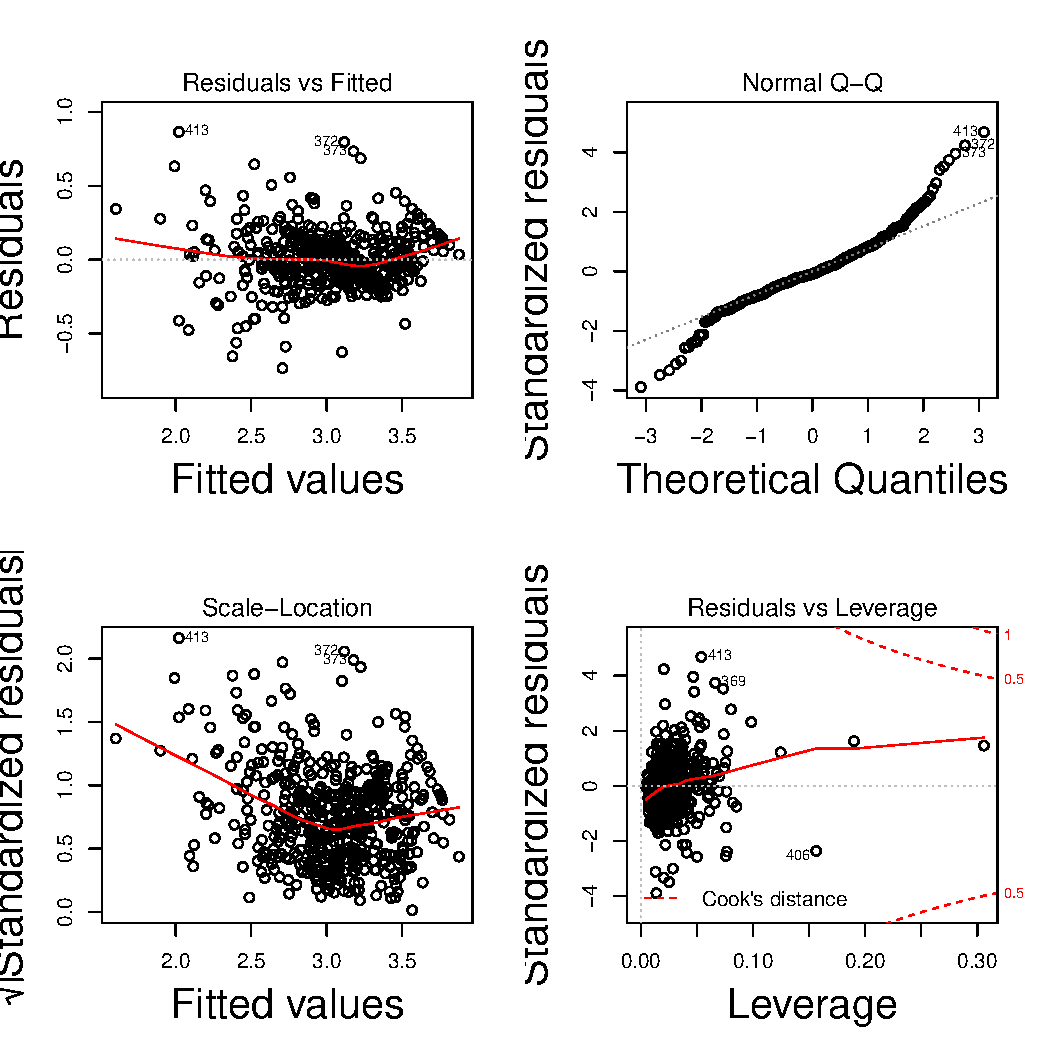
\includegraphics[width = 7.5cm]{figures/BHlindiag.pdf}
\end{center}
\end{frame}	


\begin{frame}[fragile]
\frametitle{}

Model~\eqref{housing.model.2} (inspired by \citeNP{Bels:Kuh:Wels:1980}):
\begin{eqnarray}
\label{housing.model.2}
\lefteqn{\log(\texttt{medv}) = \beta_0 + \beta_1\texttt{crim} + \beta_2\texttt{zn}+
\beta_3\texttt{indus}+ }\nonumber \\
& + & \beta_4\texttt{nox}{\color{blue}^2} + \beta_5\texttt{rm}{\color{blue}^2} + \beta_6\texttt{age} +
\beta_7 {\color{blue}\log}(\texttt{dis}) + \beta_8 {\color{blue}\log}(\texttt{rad}) \nonumber  \\
& + & \beta_9\texttt{tax} + \beta_{10}\texttt{ptratio} + \beta_{11}\texttt{b} +
\beta_{12} {\color{blue}\log}(\texttt{lstat})\nonumber  \\
& + & \beta_{13} \texttt{chas} + \epsilon.
\end{eqnarray}

\bs

{\scriptsize
\begin{lstlisting}
> linearfit2 <- lm(log(medv)~chas+crim+zn+indus+I(nox^2)+
   I(rm^2)+age+log(dis)+log(rad)+tax+ptratio+b+log(lstat),
   data=BostonHousing)
> summary(linearfit2)
\end{lstlisting}
}
\end{frame}

\begin{frame}[fragile]

{\scriptsize
\begin{lstlisting}
Coefficients:
              Estimate Std. Error t value Pr(>|t|)    
(Intercept)  4.558e+00  1.544e-01  29.512  < 2e-16 ***
chas         9.140e-02  3.320e-02   2.753 0.006129 ** 
crim        -1.186e-02  1.245e-03  -9.532  < 2e-16 ***
zn           8.016e-05  5.056e-04   0.159 0.874105    
indus        2.395e-04  2.364e-03   0.101 0.919318    
I(nox^2)    -6.380e-01  1.131e-01  -5.639 2.88e-08 ***
I(rm^2)      6.328e-03  1.312e-03   4.823 1.89e-06 ***
age          9.074e-05  5.263e-04   0.172 0.863179    
log(dis)    -1.913e-01  3.339e-02  -5.727 1.78e-08 ***
log(rad)     9.571e-02  1.913e-02   5.002 7.91e-07 ***
tax         -4.203e-04  1.227e-04  -3.426 0.000664 ***
ptratio     -3.112e-02  5.013e-03  -6.208 1.14e-09 ***
b            3.637e-04  1.031e-04   3.527 0.000460 ***
log(lstat)  -3.712e-01  2.501e-02 -14.841  < 2e-16 ***
---
Signif. codes:  0 ‘***’ 0.001 ‘**’ 0.01 ‘*’ 0.05 ‘.’ 0.1 ‘ ’ 1

Residual standard error: 0.1825 on 492 degrees of freedom
Multiple R-squared:  0.8059,	Adjusted R-squared:  0.8008 
F-statistic: 157.1 on 13 and 492 DF,  p-value: < 2.2e-16
\end{lstlisting}
}
\end{frame}


\begin{frame}
\frametitle{}

 \begin{center}
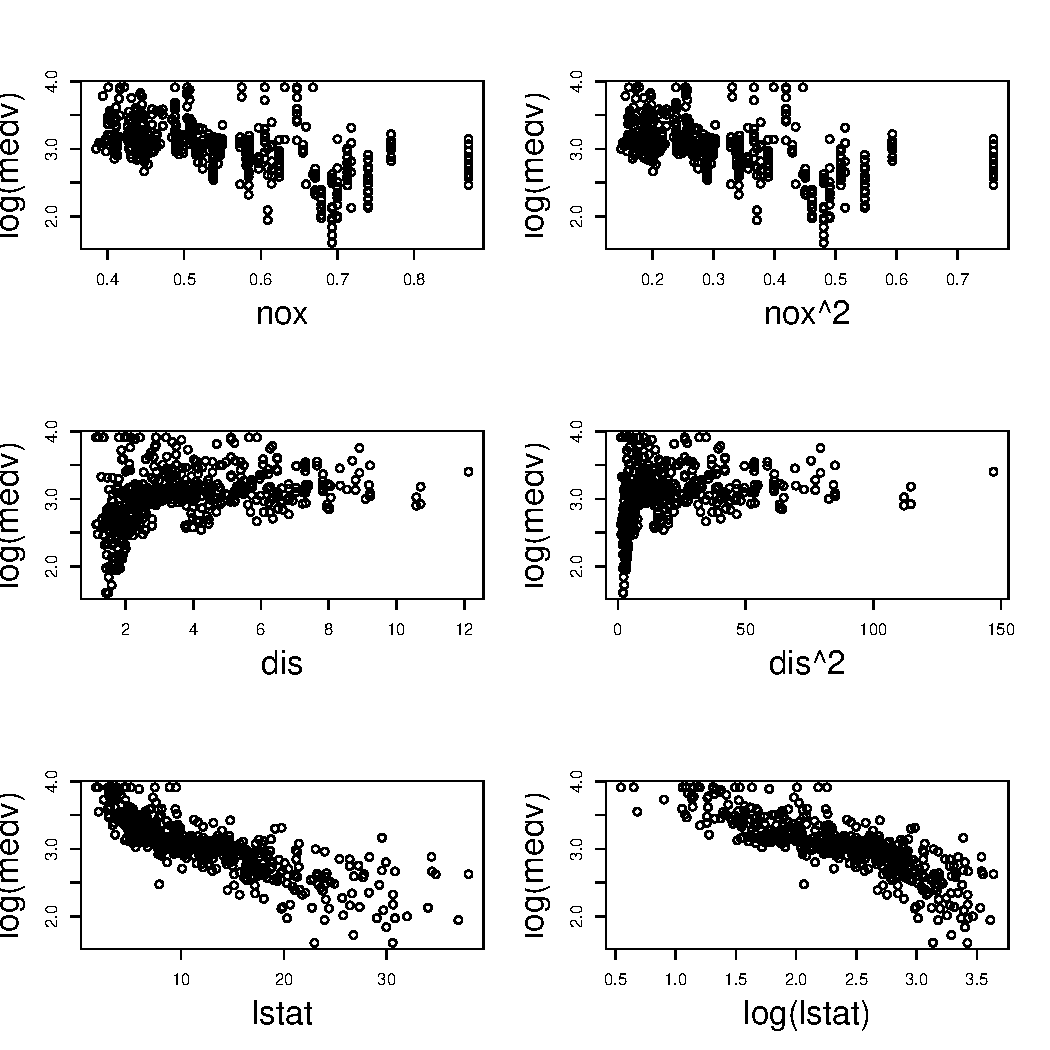
\includegraphics[width = 7.5cm]{figures/BHlin2.pdf}  
\end{center}
\end{frame}	


\begin{frame}[fragile]
\frametitle{}

Model~\eqref{housing.model.np}, nonparametric:
\begin{eqnarray*}
\label{housing.model.np}
\lefteqn{\log(\texttt{medv}) = \alpha + f_1(\texttt{crim}) + f_2(\texttt{zn})+
f_3(\texttt{indus}) +} \\
& + & f_4(\texttt{nox}) + f_5(\texttt{rm}) +  f_6(\texttt{age}) +
f_7(\texttt{dis}) + \\
& + & f_8(\texttt{rad}) + f_9(\texttt{tax}) + f_{10}(\texttt{ptratio}) \nonumber\\
& + & f_{11}(\texttt{b}) + f_{12}(\texttt{lstat}) + \beta \texttt{chas} +
\epsilon.
\end{eqnarray*}

\bs

{\scriptsize
\begin{lstlisting}
> library(mgcv)
> BHnpfit.new <- gam(log(medv)~chas+s(crim)+s(zn)+s(indus)+ 
  s(nox,k=20)+ s(rm)+s(age)+s(dis,k=20)+s(rad,k=8)+s(tax)+s(ptratio)+
   s(b)+s(lstat), data=BostonHousing)
> plot(BHnpfit.new, scale=0, page=1)
\end{lstlisting}
}

\bs 

{\color{red} $\bigstar$ Variable selection by nonnegative garrote, see
\citeN{Brei:1995} and
\citeN{Cant:Flem:Ronc:2011}.}
\end{frame}



\begin{frame}
\frametitle{}
 \begin{center}
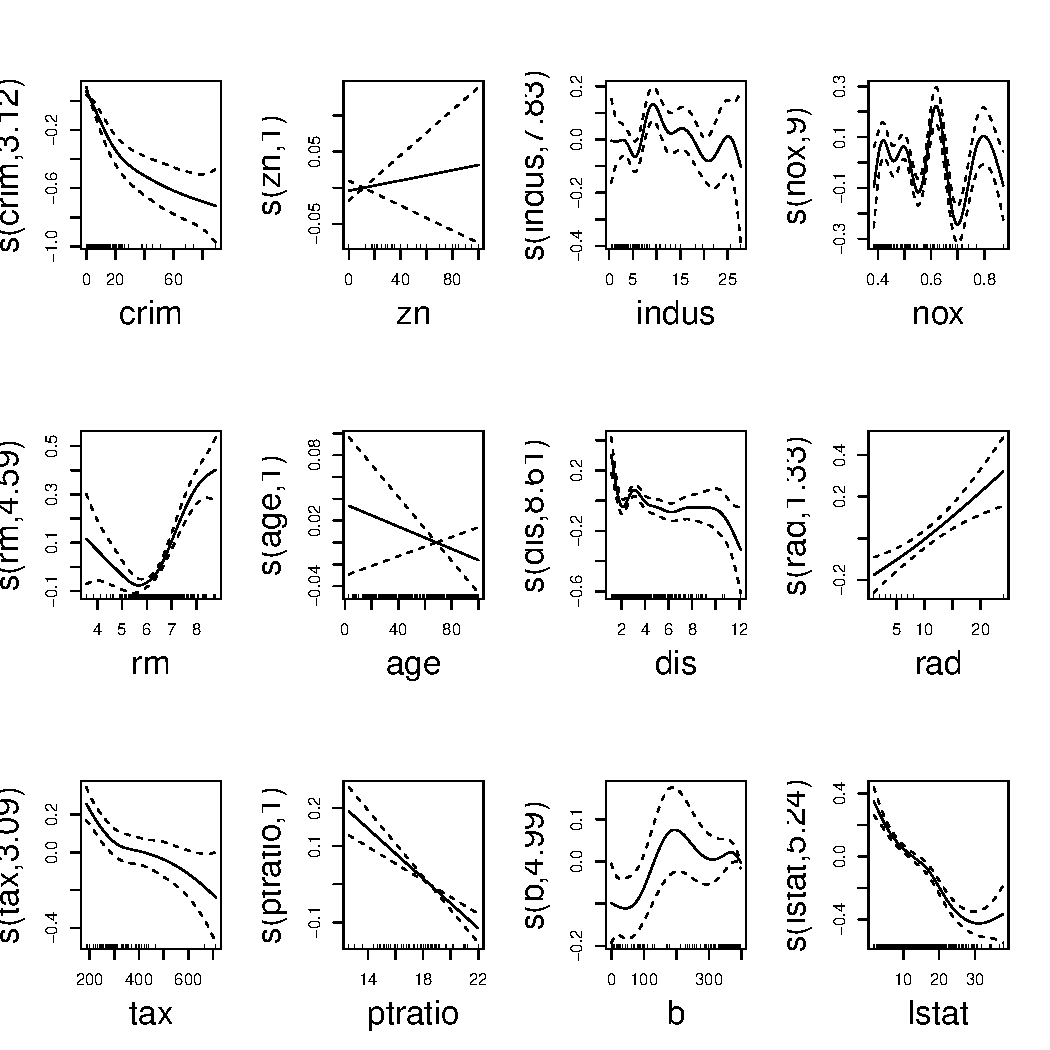
\includegraphics[width = 7.8cm]{figures/BHnpfit.pdf}  
\end{center}
\end{frame}	

\subsection{Example 2: Breast cancer diagnostic}

\begin{frame}
\frametitle{Example 2: Breast cancer diagnostic}

\label{example2}

Breast cancer diagnosis through breast cytology (fine needle aspiration instead
of invasive surgery). 

\bs
Breast cancer Wisconsin data, available from the University of
California at Irvine Repository Of Machine Learning Database
\url{www.ics.uci.edu/~mlearn/MLRepository.html}.

\bs

Outcome: 2 classes: benign (coded 0) or malignant (coded 1).

\bs

There are 699 patients on the study, 16 of which have one or more missing
value(s) in the predictors.
\end{frame}	


\begin{frame}
\frametitle{}

Available predictors:
\begin{itemize}
\item  Clump Thickness (1-10)
\item  Uniformity of Cell Size (1-10)
\item  Uniformity of Cell Shape (1-10)
\item  Marginal Adhesion (1-10)
\item  Single Epithelial Cell Size (1-10)
\item  Bare Nuclei  (1-10)
\item  Bland Chromatin (1-10)
\item  Normal Nucleoli (1-10)
\item  Mitoses (1-10)
\end{itemize}

\end{frame}



\begin{frame}[fragile]
\frametitle{}

We consider a logistic linear model.

\bs

{\scriptsize
\begin{lstlisting}
> breast.fit <- glm(status~clump+cellsize+cellshape+adhesion+
singlesize+nuclei+chromatin+nucleoli+mitoses,data=breast,
family=binomial,na.action=na.omit)
> fitted.breast <- predict(breast.fit,type="response")
> plot(fitted.breast,na.omit(breast)$status,
  xlab="Fitted values",ylab="Status")
\end{lstlisting}
}

\begin{center}
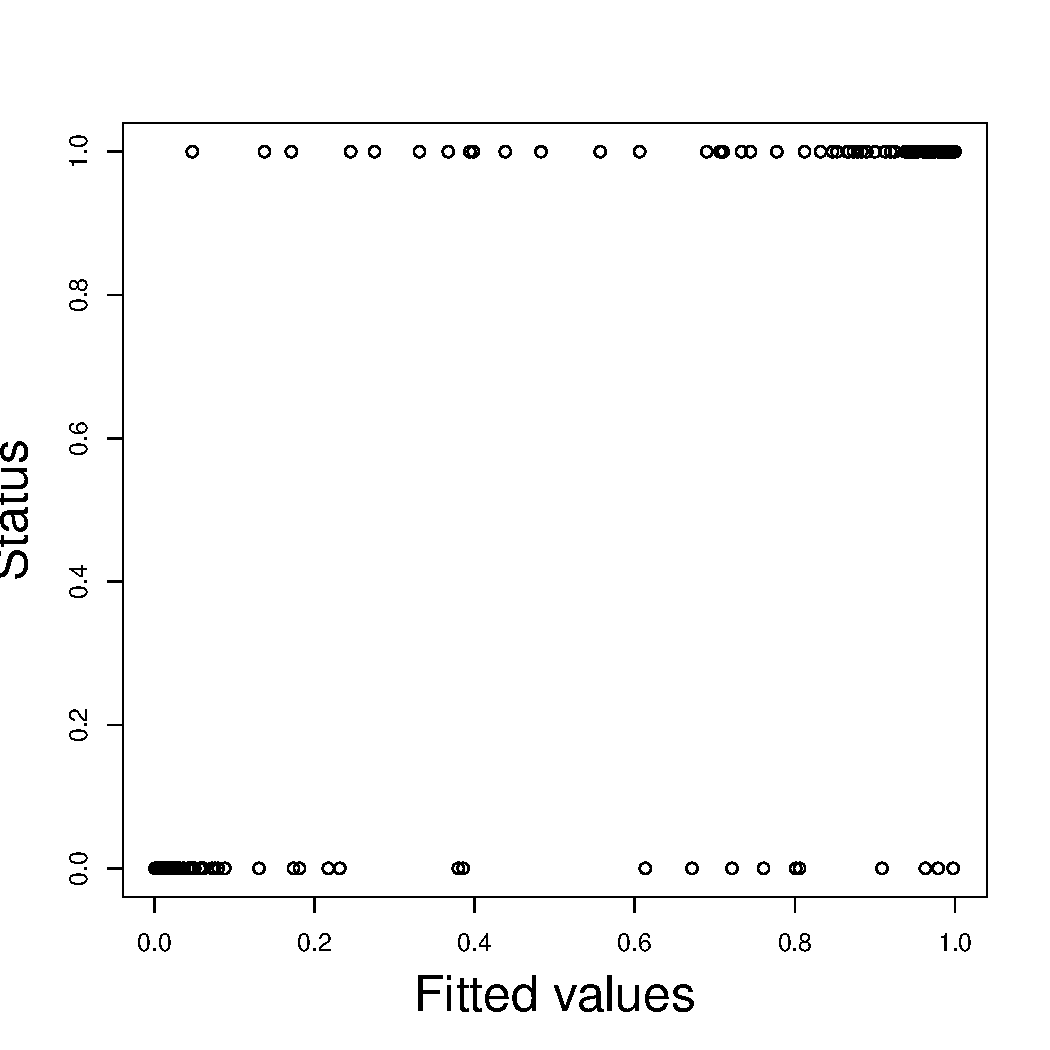
\includegraphics[width = 4.8cm]{figures/breastfitted.pdf}  
\end{center}

\end{frame}


\subsection{Example 3: Air Pollution Study}

\begin{frame}
\frametitle{Example 3: Air Pollution Study}

Data from the National Morbidity, Mortality and Air Pollution Study Database
(NMMAPS) available at \url{http://www.ihapss.jhsph.edu} for
the 88 largest metropolitan areas in the United States.

\bs

Outcome is the number of death on a day (\texttt{death}), that we
model as a Poisson variable.
\end{frame}

\begin{frame}
\frametitle{}

Potentially interesting explanatory variables:
\begin{itemize}
\item particulate matter less than 10 $\mu$m in aerodynamic diameter,
10\%-trimmed mean over all monitors in a county (\texttt{pm10tmean})
\item average temperature (over 24 hours) (\texttt{tmean})
\item time (\texttt{day})
\item dew point temperature (\texttt{dptp})
\item day of the week (\texttt{dow}: 1=Sat, 2=Sun, ...)
\end{itemize}

\bs

Main interest is in the effect of \texttt{pm10tmean} (pollution), that enters
linearly in the model.
\end{frame}


\begin{frame}[fragile]
\frametitle{San Francisco, 1st Jan., 1987 to 31st Dec, 2000,
$n=15342$}

{\scriptsize
\begin{lstlisting}
sanFfit <- gam(death~pm10tmean+s(tmean)+s(day)+s(dptp)+factor(dow),
data=sanF,family=poisson)

 Parametric coefficients:
               Estimate Std. Error z value Pr(>|z|)    
(Intercept)   1.7820648  0.0245328  72.640  < 2e-16 ***
pm10tmean     0.0017404  0.0005446   3.196  0.00139 ** 
factor(dow)2 -0.0261762  0.0349350  -0.749  0.45369    
factor(dow)3  0.0194925  0.0343809   0.567  0.57074    
factor(dow)4 -0.0207042  0.0348386  -0.594  0.55232    
factor(dow)5 -0.0013170  0.0346407  -0.038  0.96967    
factor(dow)6 -0.0002978  0.0346081  -0.009  0.99314    
factor(dow)7 -0.0140022  0.0345012  -0.406  0.68486    
---
Signif. codes:  0 ‘***’ 0.001 ‘**’ 0.01 ‘*’ 0.05 ‘.’ 0.1 ‘ ’ 1
\end{lstlisting}
}
\end{frame}

\begin{frame}[fragile]
\frametitle{}

\bs
{\scriptsize
\begin{lstlisting}
Approximate significance of smooth terms:
           edf Ref.df Chi.sq  p-value    
s(tmean) 1.973  2.568  7.642   0.0388 *  
s(day)   2.241  2.796 24.476 2.14e-05 ***
s(dptp)  1.003  1.006  0.494   0.4830    
---
Signif. codes:  0 ‘***’ 0.001 ‘**’ 0.01 ‘*’ 0.05 ‘.’ 0.1 ‘ ’ 1

R-sq.(adj) =  0.0145   Deviance explained = 2.03%
UBRE = 0.74149  Scale est. = 1         n = 1986
\end{lstlisting}
}
\end{frame}

\begin{frame}
\frametitle{}

\begin{center}
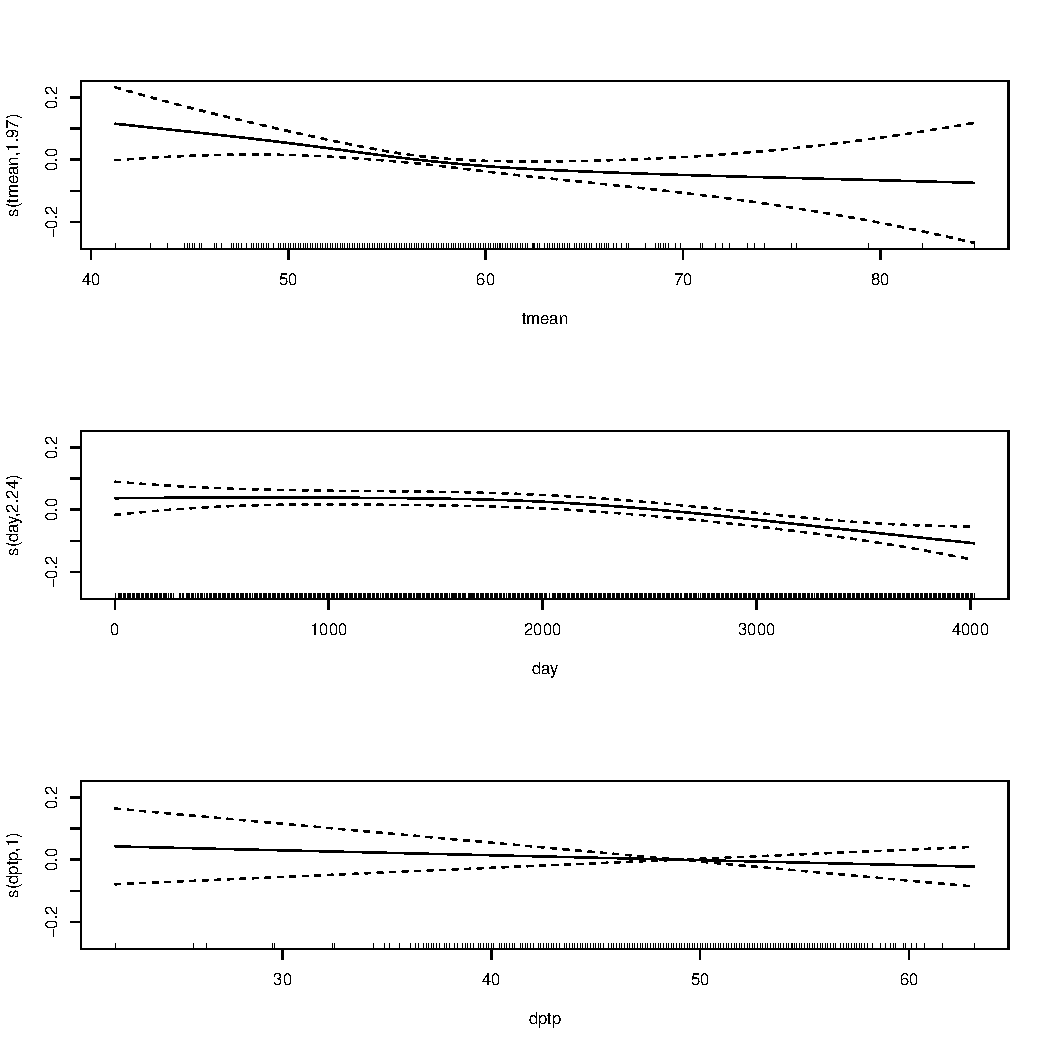
\includegraphics[width = 7.5cm]{figures/NMMAPSfit.pdf}  
\end{center}

\end{frame}


\begin{frame}
\frametitle{}
\begin{center}
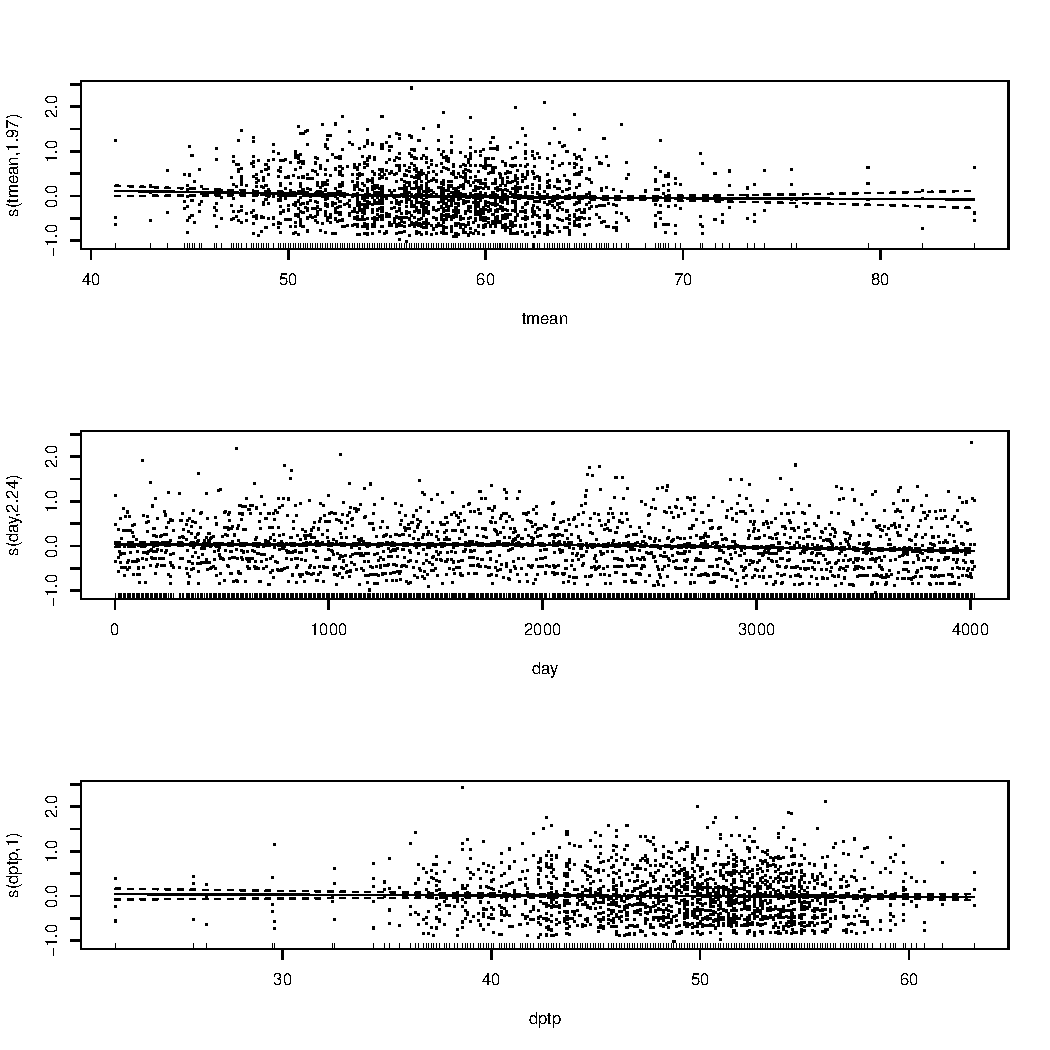
\includegraphics[width = 4cm]{figures/NMMAPSfitwithres.pdf}  
\end{center}

Open questions:
\begin{itemize}
\item Are all the terms significant?
\item Other factors impacting the number of deaths.

($R^2$ and explained deviance low because few explanatory variables.)
\item {\color{red} $\bigstar$ Different models for different age groups (see
\citeNP{Domi:Same:Zege:2000})}.
\end{itemize}
\end{frame}

\subsection{Example 4: Cost of stay for back problems}
\label{CHUV.Ex}

\begin{frame}
\frametitle{Example 4: Cost of stay for back problems}

100 patients hospitalized at the \textit{Centre Hospitalier
Universitaire Vaudois (CHUV)} in Lausanne (Switzerland) during 1999 for
``medical back problems'' (APDRG 243). 

\sms
Data provided by A.\ Marazzi, see
\citeN{Mara:Yoha:2004}.

\bs
\bs

The outcome is the cost of stay (\texttt{CouTot} in Swiss
francs) 
\end{frame}


\begin{frame}
\frametitle{}
Explanatory variables:
\begin{itemize}
\item length of stay (\texttt{LOS}, in days)
\item admission type (\texttt{Typadm}: 0=planned, 1=emergency)
\item insurance type (\texttt{TypAss}: 0=regular, 1=private)
\item age in years (\texttt{age})
\item sex (\texttt{Sexe}: 0=female, 1=male)
\item discharge destination (\texttt{dest}:
1=home, 0=another health institution)
\end{itemize}

\bs

Goals:
\begin{itemize}
\item Identify factor impacting cost of stay
\item Prediction
\end{itemize}
\end{frame}


\begin{frame}
\frametitle{}

\begin{center}
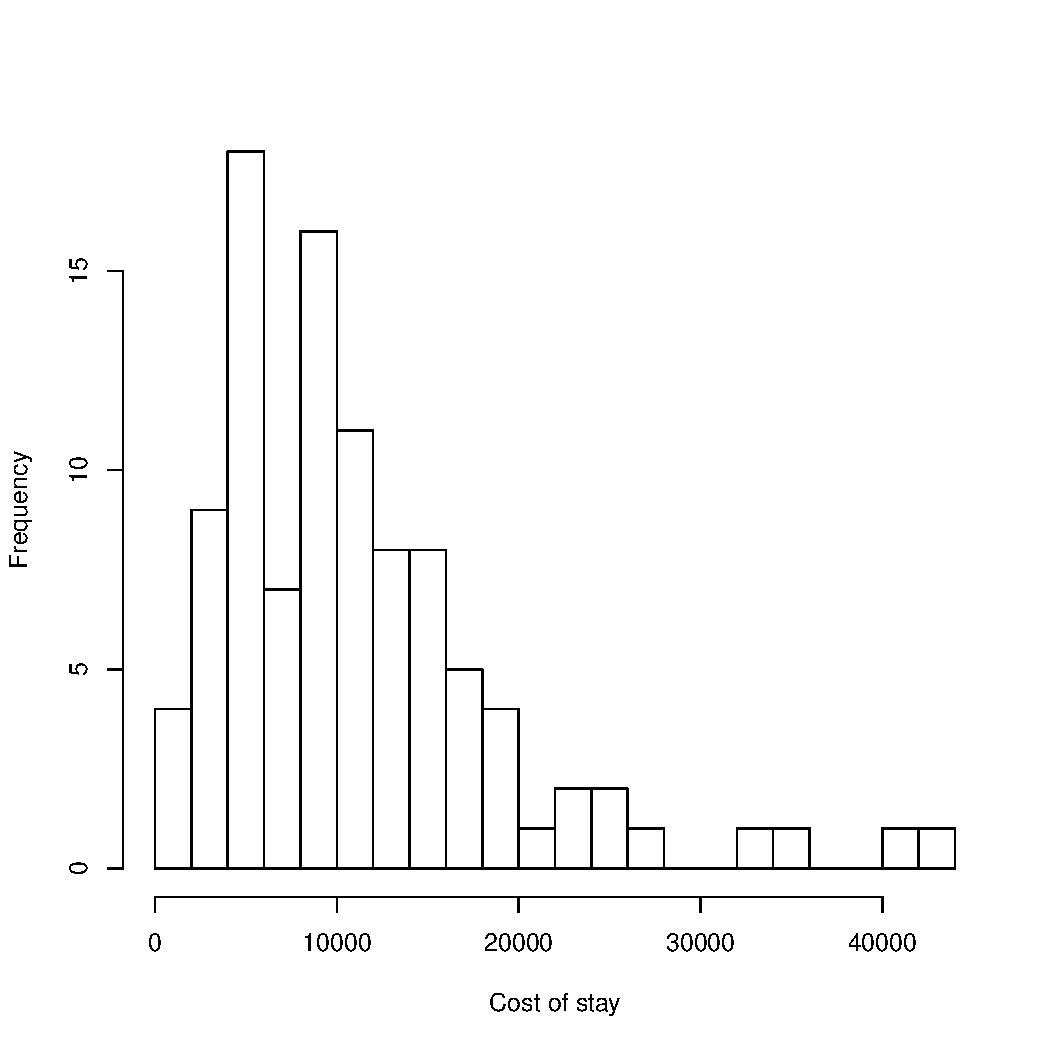
\includegraphics[width = 8cm]{figures/CostCHUV.pdf}  
\end{center}

\end{frame}

\begin{frame}[fragile]
\frametitle{Gamma model with logarithmic link.}

{\scriptsize
\begin{lstlisting}
Coefficients:
              Estimate Std. Error t value Pr(>|t|)    
(Intercept)  7.2338121  0.1468364  49.264  < 2e-16 ***
log(LOS)     0.8222203  0.0279641  29.403  < 2e-16 ***
Typadm       0.2136148  0.0500028   4.272 4.67e-05 ***
Typass       0.0932763  0.0791100   1.179   0.2414    
age         -0.0005335  0.0012852  -0.415   0.6790    
Sexe         0.0951009  0.0499814   1.903   0.0602 .  
dest        -0.1043560  0.0692713  -1.506   0.1353    
---
Signif. codes:  0 ‘***’ 0.001 ‘**’ 0.01 ‘*’ 0.05 ‘.’ 0.1 ‘ ’ 1

(Dispersion parameter for Gamma family taken to be 0.04961642)

    Null deviance: 47.9536  on 99  degrees of freedom
Residual deviance:  5.0718  on 93  degrees of freedom
AIC: 1817.9

Number of Fisher Scoring iterations: 5
\end{lstlisting}
}
\end{frame}

\begin{frame}
\frametitle{}

\begin{center}
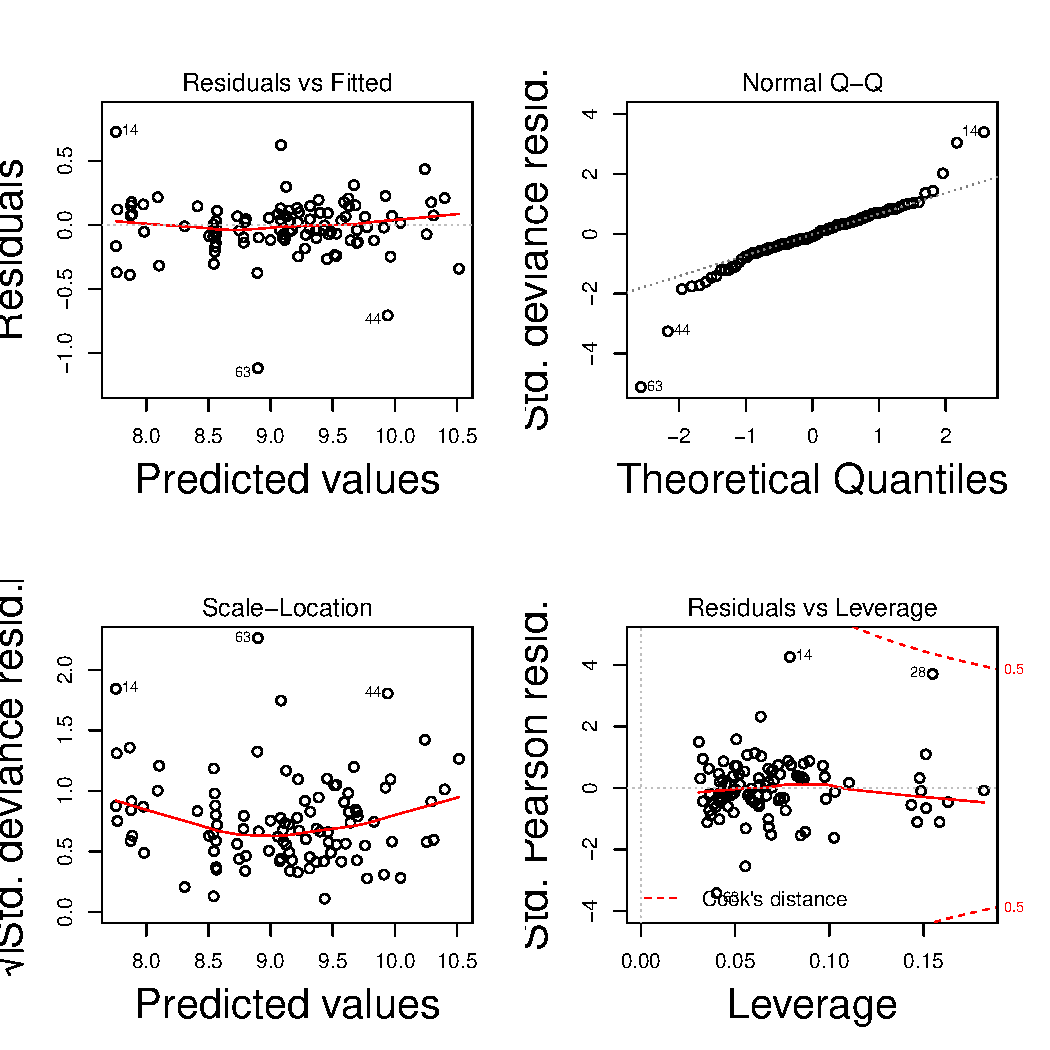
\includegraphics[width = 6.5cm]{figures/MYdiag.pdf}  
\end{center}

Outliers! (see Chapter~\ref{robust.section})
\end{frame}

\subsection{Example 5: CARDIA study}

\begin{frame}
\frametitle{Example 5: CARDIA study}

Data from the CARDIA study (Coronary Artery Risk Development in young
Adults), available from the JASA data archive at
\url{http://lib.stat.cmu.edu/jasadata/}, see \citeN{Prei:Gale:Lohm:Wage:2000}.

\label{CARDIApage}
\bs

5'115 adults aged 18-30 years were followed and examined up to 5 times  from
1986 to 1996 at years 0, 2, 5, 7 and 10.

\bs

We consider the subsample of 3693 individuals for which we have full information
for the first 4 visits (no missing values).

\bs

Outcome (at each visit): self-reported smoking status (yes/no, coded 1/0).
\end{frame}


\begin{frame}
\frametitle{}


Predictors (at each visit):
\begin{itemize}
\item age (time dependent)
\item birth cohort (1955-1962,1963-1967) (time independent)
\item education (high school or less, some college, college degree) (time
(in)dependent)
\item racesex (black males, black females, white males, white females) (time
independent)
\end{itemize}

\vfill
{\color{red} $\bigstar$ Missingness issues, see \citeN{Prei:Gale:Lohm:Wage:2000}}.
\end{frame}

\begin{frame}[fragile]
\frametitle{}
{\tiny
\begin{lstlisting}
Call:
gee(formula = smoke ~ age + factor(birth) + factor(education) + 
    factor(racesex), id = id, data = CARDIA.sub, family = binomial, 
    corstr = "exchangeable")

Summary of Residuals:
       Min         1Q     Median         3Q        Max 
-0.5506120 -0.3121130 -0.1189440  0.4816228  0.9095992 

Coefficients:
                      Estimate Naive S.E.    Naive z Robust S.E.   Robust z
(Intercept)        -1.33707777 0.54231807  -2.465486  0.54510289  -2.452891
age                 0.06480087 0.02646754   2.448315  0.02669744   2.427231
factor(birth)2     -0.19856466 0.14606724  -1.359406  0.14563751  -1.363417
factor(birth)3     -0.40380459 0.23689643  -1.704562  0.23858001  -1.692533
factor(education)2 -0.68712005 0.08313860  -8.264754  0.08490269  -8.093030
factor(education)3 -1.96140806 0.10016299 -19.582164  0.10054908 -19.506972
factor(racesex)2   -0.17668132 0.09763816  -1.809552  0.09900202  -1.784623
factor(racesex)3   -0.13445604 0.10634023  -1.264395  0.10833799  -1.241079
factor(racesex)4   -0.12730906 0.10530815  -1.208919  0.10599195  -1.201120

Estimated Scale Parameter:  1.000362
Number of Iterations:  1

Working Correlation
         [,1]     [,2]     [,3]     [,4]
[1,] 1.000000 0.727139 0.727139 0.727139
[2,] 0.727139 1.000000 0.727139 0.727139
[3,] 0.727139 0.727139 1.000000 0.727139
[4,] 0.727139 0.727139 0.727139 1.000000
\end{lstlisting}
}
\end{frame}


\subsection{Example 6: Birds abundance}

\begin{frame}
\frametitle{Example 6: Birds abundance}


Are birds counts decreasing? Abundance of animal species.

\bs

The example of 5 species of Seal Island (Nova Scotia,
Canada) that winters mostly in the Southern USA: Northern Flicker, Red-wing Blackbird, Rusty Blackbird,
Ruby-crowned Kinglet, Yellow-rumped Warbler.

\bs

Data courtesy of Prof.\ I. MacLaren, Dalhousie University.


\bs

2245 observations (autumn season, between Aug.\ 1st and Nov.\ 14th, over 40 years
since 1963), that is 449 days of observations for each bird species.

\end{frame}

%\begin{figure}[bp]
%\centerline{\epsfig{figure=figures/observers.ps,height=18cm}}
%\caption{Days when observer(s) were present on Seal Island.}
%\label{observer.fig}
%\end{figure}


\begin{frame}
\frametitle{}
\begin{tabular}{ccc}
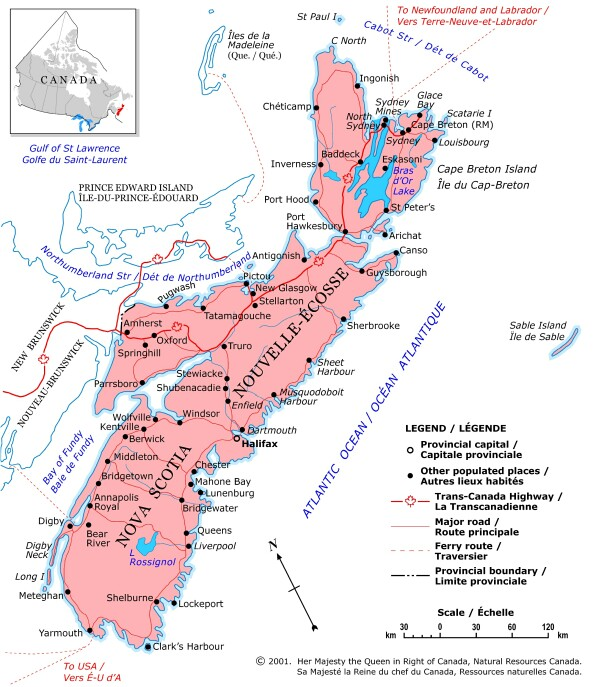
\includegraphics[width = 3.5cm]{figures/novascotia.jpg}   & 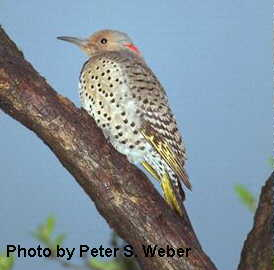
\includegraphics[width = 2.5cm]{figures/northernflicker.jpg}  & 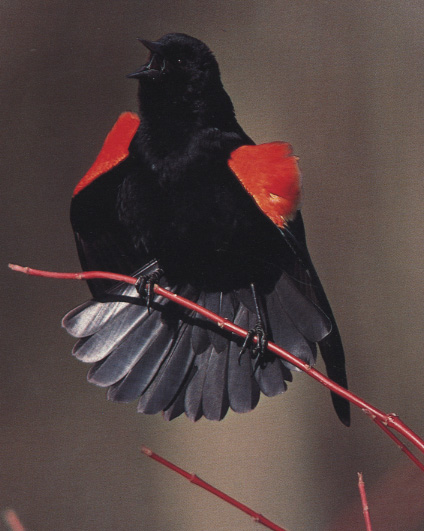
\includegraphics[width = 2.5cm]{figures/redwing2.jpg} \\
 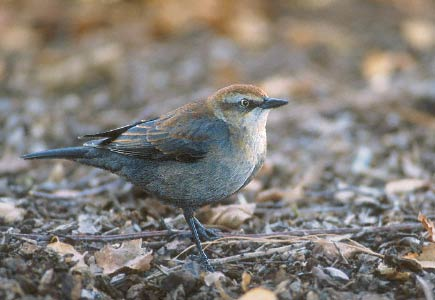
\includegraphics[width = 2.5cm]{figures/rustyblackbird.jpg}  & 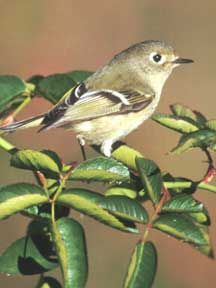
\includegraphics[width = 2.5cm]{figures/ruby_crowned_kinglet.jpg} & 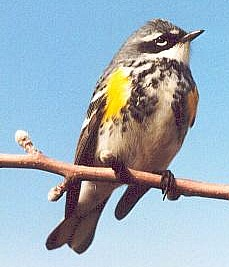
\includegraphics[width = 2.5cm]{figures/Yellow_rumped_Warbler.jpg} 
\end{tabular}

\end{frame}
\begin{frame}
\frametitle{}

Outcome: Number of birds observed (counts, \texttt{NUMBER}).

\bs
Predictors:
\begin{itemize}
\item year (\texttt{YEAR})  - {\color{blue}Main interest}.
\item day (\texttt{DAY}) 
\item number
of observer on the island (\texttt{NO.OBS}) 
\item wind direction at midnight the night before (\texttt{WIND.0}) 
\item wind direction at noon the day before (\texttt{WIND.1}) 
\item wind direction at midnight 2 days before (\texttt{WIND.2}) 
\item wind direction at noon 2 days before (\texttt{WIND.3}) 
\item the speed of the wind that day (\texttt{WINDSPD}) 
\item sky condition (1=clear, 2=cloudy, 3=fog, 4=rain) (\texttt{SKY})
\item proportion of illuminated moon (\texttt{MOON}) 
\item bird species (1-5) (\texttt{BIRD})
\end{itemize}

\end{frame}


\begin{frame}[fragile]
\frametitle{}
Poisson model with logarithmic link:
\begin{eqnarray*}
\lefteqn{\texttt{NUMBER} \sim  \alpha + f_1(\texttt{YEAR}) + f_2(\texttt{DAY}) +
f_3(\texttt{NO.OBS})} \\
& + & f_4(\texttt{WIND.0}) + f_5(\texttt{WIND.1}) +
f_6(\texttt{WIND.2}) \\
& + & f_7(\texttt{WIND.3}) + f_8(\texttt{WINDSPD}) +
\mbox{factor(\texttt{SKY})}\\
& + & f_9(\texttt{MOON}) + \mbox{factor}(\texttt{BIRD})
\end{eqnarray*}

\bs

{\scriptsize
\begin{lstlisting}
> require(mgcv)
> GrA.fit <- gam(NUMBER~s(YEAR,k=20)+s(DAY,k=20)+s(NO.OBS,k=8)+
   s(WIND.0,k=20)+s(WIND.1,k=20)+s(WIND.2,k=20)+s(WIND.3,k=20)+
   s(WINDSPD,k=20)+factor(SKY)+s(MOON,k=20)+factor(BIRD), 
   family=poisson,data=GrA,na.action=na.omit)
> plot(GrA.fit,scale=0,pages=1,pers=T,all.terms=T,cex.lab=2)
\end{lstlisting}}
\end{frame}

\begin{frame}
\frametitle{}

\begin{center}
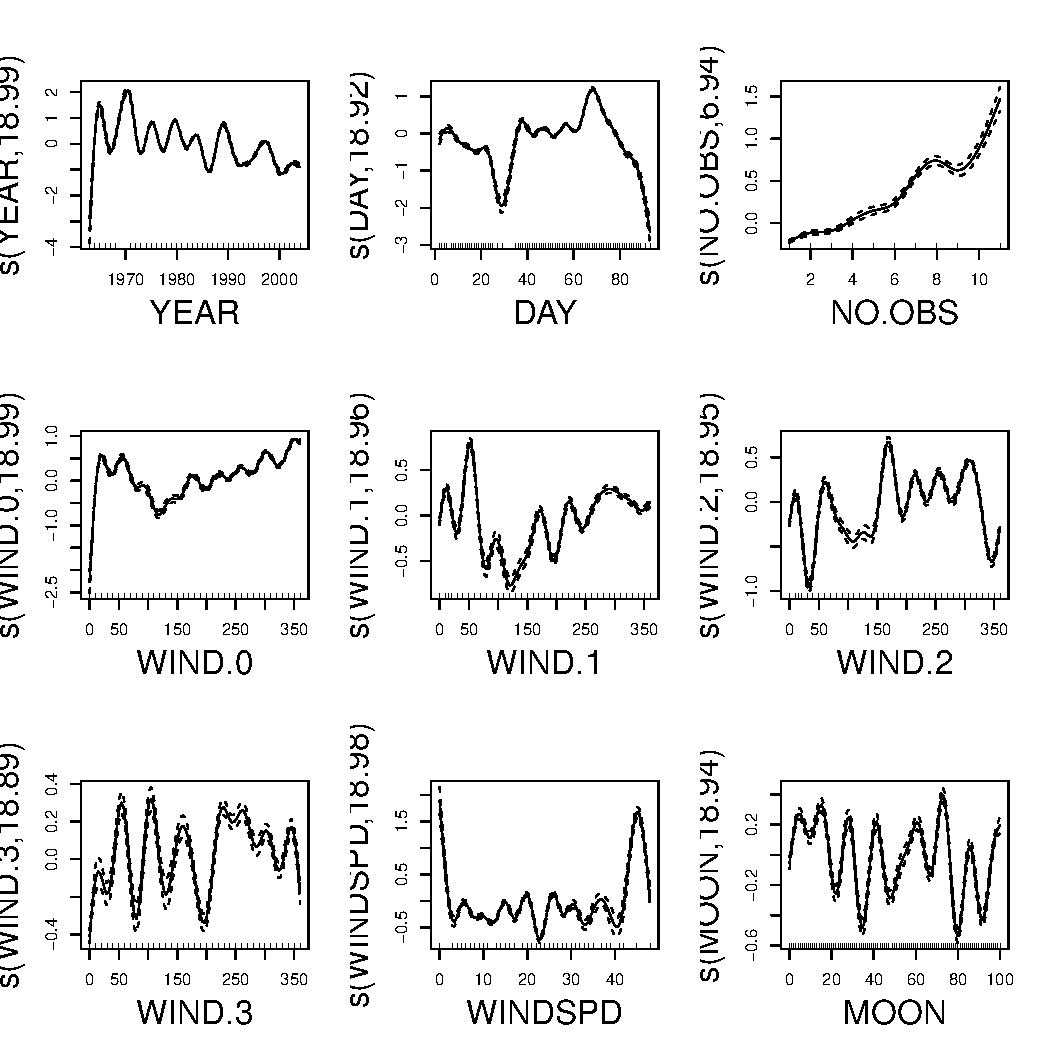
\includegraphics[width = 6.5cm]{figures/GrA.pdf}  
\end{center}
\vfill{\color{red} $\bigstar$ Possible excess of zeros. Review: \citeN{Rido:Deme:Hind:1998}}
\end{frame}

\subsection{Summary}

\begin{frame}
\frametitle{What do Examples 1 to 6 have in common?}


{\color{blue}
Same general model formulation:
$$g(E(Y_i)) = g(\mu_i) = $$
$$= \eta_i = \left\{
   \begin{array}{l}
   \beta_0 + \beta_1 x_{i1}+\ldots+\beta_p x_{ip} \\
  \alpha + f_1(x_{i1})+ \ldots + f_p(x_{ip})
  \end{array} \right.$$}

\bs

$g$ is called the link function.

\bs

$\eta_i$ is called the linear (additive) predictor.

\end{frame}

\begin{frame}
\frametitle{Notation}

{\color{blue}Outcome (response) variable}: \\
observations $y_1, \ldots, y_n$
for $n$ individuals (or subjects) corresponding to random variables $Y_1,
\ldots, Y_n$.

\bs

$y_i$ (resp.\ $Y_i$) can be multidimensional, in which case
we will denote its elements as $y_{it}$ with $t=1,\ldots,n_i$.

\bs

{\color{blue}Distribution properties of $Y_i$}:

$Y_i$ issued from a distribution $F_{\theta_i}$:
$$Y_i \sim F_{\theta_i}$$
We denote expectation $E(Y_i) = \mu_i$ and variance $Var(Y_i) = v_i$.
\end{frame}

\begin{frame}
\frametitle{}

{\color{blue}Explanatory variables (predictors)}:
\begin{itemize}
\item for unidimensional $y_i$:
$$x_i = (x_{i0}, x_{i1}, \ldots, x_{ip})^T$$
is a vector of dimension $(p+1)$. $x_{i0}$ usually equal to 1
(intercept). Combined information:
$$X =  \left( \begin{array}{c}
x_1^T\\
\vdots \\
x_n^T
\end{array} \right) =
\left(
\begin{array}{cccc}
x_{10} & x_{11} & \cdots & x_{1p}\\
x_{20} & x_{21} & \cdots & x_{2p}\\
\vdots & \vdots & \vdots & \vdots \\
x_{n0} & x_{n1} & \cdots & x_{np}\\
\end{array} \right)
$$

\label{Ximatrix}
\end{itemize}
\end{frame}

\begin{frame}
\frametitle{}

\begin{itemize}
\item for multidimensional $y_i$:
$$X_i = \left(
\begin{array}{cccc}
x_{i10} & x_{i11} & \cdots & x_{i1p}\\
x_{i20} & x_{i21} & \cdots & x_{i2p}\\
\vdots & \vdots & \vdots & \vdots \\
x_{in_i0} & x_{in_i1} & \cdots & x_{in_ip}\\
\end{array} \right)$$
\end{itemize}

Combined information:
$$X = \left(
\begin{array}{c}
X_1 \\
X_2 \\
\vdots\\
X_n
\end{array} \right) $$
\end{frame}

\begin{frame}
\frametitle{Background and prerequisite}


Familiarity with the following concepts:
\begin{itemize}
\item Estimation (maximum likelihood, least squa\-res, method of moments, etc.)
\item Confidence intervals.
\item Sampling distributions.
\item Hypotheses testing (null and alternative hypothesis, test statistic and
its distribution, p-value, significance level, etc.).
\item Linear regression.
\item Calculus and matrix notation.
\item $\ldots$
\end{itemize}

\end{frame}


\begin{frame}[allowframebreaks]
\frametitle{Principles of statistical modelling}

\bs 

A statistical analysis should include the following steps:
\begin{enumerate}
\item {\color{blue}Exploratory data analysis} to check data quality and to help
with model formulation. Consider each variable separately and consider the
following questions:
\begin{itemize}
\item What is the scale of measurements?
\item What is the shape of the distribution?
\item How is it associated with other variables?
\end{itemize}
\item {\color{blue}Model formulation}:
  \begin{itemize}
  \item Probability distribution of $Y$.
  \item Link with the explanatory variables.
  \end{itemize}
\item {\color{blue}Parameter estimation}: which method? (maximum likelihood,
least squares, method of moments, etc.)
\newpage
\item {\color{blue}Residuals and model checking}:
  \begin{itemize}
  \item Graphical inspections of residuals (independence, approximate normality, zero mean, constant variance).
  \item Goodness of fit tests.
  \end{itemize}
\item {\color{blue}Inference and interpretation}:\\
Test hypothesis about parameters to obtain a parsimonious model. Then (and only
then) interpret parameters.
\end{enumerate}

\end{frame}


\section{Generalized Linear Models (GLM)}

\begin{frame}
\frametitle{Generalized Linear Models (GLM)}
Class of models unified by \citeN{Neld:Wedd:1972} (see \citeNP{McCu:Neld:1989}).

\bs

The well known {\color{blue}linear model} is often written
$$Y_i = x_i^T \beta + \epsilon_i,$$
with $\epsilon_i \sim {\mathcal N}(0,\sigma^2)$ and hence $Y_i \sim {\mathcal N}(\mu_i,\sigma^2)$.

The same model can also be written as
$$E(Y_i) = \mu_i = x_i^T \beta.$$
\end{frame}

\begin{frame}
Generalized linear models include more general situations:
\begin{enumerate}
\item Response variables that have distributions other than the Normal
  distribution (even discrete or categorical).
\item Relationship between the response and the explanatory variables
  need not be of the simple linear form above.
\end{enumerate}

The general form of a GLM is:
$${\color{blue}g(E(Y_i)) = g(\mu_i)=\eta_i=x_i^T \beta},$$
where $g$ is called the link function. We denote $Var(Y_i) = v_i = v(\mu_i)$.

\end{frame}


\begin{frame}
\frametitle{Examples}

\begin{itemize}
\item logistic regression:\\
 $Y_i \sim  Bernoulli(p_i)$, $E(Y_i) = p_i$
$$\log\Big(\frac{p_i}{1-p_i}\Big) = \mbox{logit}(p_i) = x_i^T \beta.$$
\item  Poisson:\\
$Y_i \sim {\mathcal P}(\lambda_i)$, $E(Y_i) = \lambda_i$
$$\log(\lambda_i) = x_i^T \beta.$$
\end{itemize}

\end{frame}

\begin{frame}
\frametitle{Limitations}

\begin{itemize}
\item the linear component is retained ( $\leadsto$ GAM, Chapter~\ref{GAM.section})
\item distributions are restricted to the exponential family (see discussion in
Section~\ref{GLM.estim.section})
\item responses must be independent ($\leadsto$ GEE, Chapter~\ref{GEE.section}
and GLMM, Chapter~\ref{GLMM.section})
\end{itemize}

\end{frame}

\subsection{Exponential family}

\begin{frame}
\frametitle{}


The unified theory of GLM is built upon the {\color{blue}exponential family} of
distributions, taking advantage of its nice properties.

\bs

\textbf{Definition}: Consider $Y$ whose distribution depends on a single
parameter $\theta$. A density or probability function is said to
belong to {\color{blue}exponential family} if it can be written in the form
$$f(y; \theta,\phi) = \exp\left( A \ \frac{y \theta - b(\theta)}{\phi} +
c(y,\frac{\phi}{A}) \right),$$ 
for some specific functions $b()$ and $c()$ and constant $A$. If $\phi$ is
known, it is an exponential family with {\color{blue}canonical parameter} $\theta$.

\bs
A link function $g$ of the GLM specification is said to be canonical if it is
such that $\theta(\mu)=\eta$, that is if $g(\cdot) = (b^{\prime})^{-1}(\cdot)$
(given that $\mu=b^{\prime}(\theta)$, see~\eqref{expect.exponential} on
page~\pageref{expect.exponential}).   
\end{frame}


\begin{frame}
\frametitle{}

\textbf{Example}: The {\color{blue} normal distribution} (where $\mu$ is the
parameter of interest and $\sigma^2$ is regarded as a nuisance
parameter)  belongs to the exponential
family. In fact:
\begin{eqnarray*}
  f(y; \mu) & = & \frac{1}{\sqrt{2\pi}\sigma} \exp\big(-\frac{1}{2
  \sigma^2}(y-\mu)^2\big)\\
& = & \exp \big( -\frac{y^2}{2 \sigma^2} + \frac{y \mu}{\sigma^2} - \frac{\mu^2}{2 \sigma^2} - \frac{1}{2} \log(2 \pi \sigma^2) \big).
\end{eqnarray*}
We identify $\theta=\mu$, $A=1$, $\phi=\sigma^ 2$, $b(\theta) = \mu^2/2=
\theta^2/2$ and
$$c(y,\phi/A) = -\frac{1}{2} \left( \frac{y^2}{\phi} + \log(2 \pi \phi) \right).$$
The canonical link is the identity function.
\end{frame}

\begin{frame}
\frametitle{}

\textbf{Example}: The {\color{blue}Poisson distribution} belongs to the
exponential family.
\begin{eqnarray*}
  f(y;\lambda) & = & \frac{\lambda^y \exp(-\lambda)}{y!}\\
& = & \exp \big(y \log(\lambda) - \lambda - \log(y!) \big),
\end{eqnarray*}
where $\theta=\log(\lambda)$, $A=1$, $\phi=1$, $b(\theta) = \lambda = \exp(\theta)$
and $c(y,\phi/A)=-\log(y!)$.

\bs
The canonical link is the log() function.
\end{frame}


\begin{frame}
\frametitle{}

\begin{table}[tbp]
  \centering
  \begin{tabular}{|l|c|c|c|c|}
   \hline
  Distribution & $A$ & $\phi$ & $b(\theta)$ & $c(y, \phi/A)$\\
  \hline
   ${\mathcal N}(\mu,\sigma^2)$ & $1$ & $\sigma^2$ &  $\theta^2/2$ & $-\frac{1}{2} (y^2/\phi + \log(2 \pi \phi))$ \\
   ${\mathcal P}(\lambda)$ & $1$ & $1$ & $\exp(\theta)$ & $-\log(y!)$ \\
   ${\mathcal B}(m,p)/m$ & & & & \\
    $\Gamma(\mu,\nu)$ & & & &\\
   \hline
  \end{tabular}
  \caption{Members of the exponential family.}
  \label{exponential.table}
\end{table}
\end{frame}

\begin{frame}
\frametitle{Properties of the exponential family}

Let us first develop general expressions for the expected value and the variance
of $Y$, useful later in this Chapter.

\bs

\textbf{Reminder}: If $l(\theta, \phi;y) = \log(f(y; \theta,\phi))$, it holds:
\begin{equation}
\label{reminder1}
E\left(\frac{\partial l(\theta, \phi;Y)}{\partial \theta}\right)=0,
\end{equation}
and
\begin{equation}
\label{reminder2}
E\left(\frac{\partial^2 l(\theta, \phi;Y)}{\partial \theta^ 2}\right) +
E\left(\left(\frac{\partial l(\theta, \phi;Y)}{\partial \theta}\right)^2\right)=0,
\end{equation}
if the order of integration and differentiation can be reversed (compact support
of the distribution).
\end{frame}


\begin{frame}
\frametitle{}


For the densities in the exponential family, we have
\begin{equation}
\label{deriv1}
\frac{\partial l(\theta, \phi;y)}{\partial \theta} = A \  \frac{y -
b^{\prime}(\theta)}{\phi},  
\end{equation}
and
\begin{equation}
\label{deriv2}
\frac{\partial^2 l(\theta, \phi;y)}{\partial \theta^2} = - A \frac{b^{\prime \prime}(\theta)}{\phi}
\end{equation}

\bs
From \eqref{reminder1} and \eqref{deriv1} we obtain
$$0=E\left(\frac{\partial l(\theta, \phi;Y)}{\partial \theta}\right)=A \
\frac{E(Y) - b^{\prime}(\theta)}{\phi}$$
which gives
\bs
\begin{equation}
\label{expect.exponential}
{\color{blue}E(Y) = \mu = b^{\prime}(\theta)}
\end{equation}
\end{frame}


\begin{frame}
\frametitle{}

Similarly, from \eqref{reminder2} and \eqref{deriv2}, and using
\eqref{expect.exponential}, we obtain

\begin{eqnarray*}
0 & = & E\left(- A \ \frac{b^{\prime \prime}(\theta)}{\phi}\right) +   E\left(
\left( A \ \frac{Y - b^{\prime}(\theta)}{\phi}\right)^2\right)\\
 & = &  - A \ \frac{b^{\prime \prime}(\theta)}{\phi} + A^2  \ E\left(
\left( \frac{Y - \mu}{\phi}\right)^2\right)\\
 & = & - \frac{b^{\prime \prime}(\theta)}{\phi} + A \ \frac{Var(Y)}{\phi^2}\\
 & = & - b^{\prime \prime}(\theta) + A \frac{Var(Y)}{\phi}
\end{eqnarray*}
\bs
which gives
\begin{equation}
\label{var.exponential}
{\color{blue}Var(Y) = \frac{b^{\prime \prime}(\theta)\phi}{ A}}
\end{equation}
\end{frame}

\subsection{GLM ingredients}

\begin{frame}
\frametitle{}

{\color{blue}Three components}:

\begin{enumerate}
\item Independent response variables $Y_1, \ldots,Y_n$ which are assumed to share
  the same distribution from the exponential family ($F_{\theta_i}$).
\item A set of parameters $\beta$ and explanatory variables $x_i^T = (1,
x_{i1},  \ldots, x_{ip})$ for $i=1,\ldots,n$.
\item A monotone and differentiable link function $g$ such that
$$g(\mu_i) = x_i^T  \beta.$$
$\eta_i = x_i^T \beta$ is called the linear predictor.
\end{enumerate}

\end{frame}

\begin{frame}
\frametitle{}

The initial problem has $n$ (=sample size) unknown parameter $\mu_1,
\ldots,\mu_n$ (or $\theta_1, \ldots, \theta_n$) which are reduced to $(p+1)$
unknown parameters ($\beta_0, \beta_1,\ldots,\beta_p$) by imposing the structure
of a GLM model.

\bs
\bs

The transformation via the link function ensures that the
estimated parameter lies in the admissible space of values
(for example, $(0,1)$ for Bernoulli/binomial and $(0, \infty)$ for Poisson).
\end{frame}

\subsection{Examples}

\begin{frame}
\frametitle{Normal distribution: $Y_i \sim {\mathcal N}(\mu_i,\sigma^2)$}


The normal distribution is used to model continuous data that have a symmetric
distribution. Examples: height or blood pressure of people. The corresponding
link function is the identity function $g(\mu_i)=\mu_i$ (no restriction on the
possible values for $\mu_i$, a linear model).

\bs
\bs

\textbf{Remark}: This model is very popular:
\begin{itemize}
\item many phenomena well described by the normal distribution
\item average or total of a random sample approximated by the normal distribution (central limit theorem)
\item a lot of theory available for this model (explicit, analytical results).
\end{itemize}
\end{frame}

\begin{frame}
\frametitle{Binomial distribution: $Y_i \sim {\mathcal B}(m_i,p_i)$}

Models a process with binary outcomes. Examples: the number of candidates who
pass a test (outcome: pass or fail), the number of patients with some disease
who are alive at a specified time since diagnosis (outcome: alive or dead), the
smoking status of a person.

\bs

For GLM we prefer to consider the proportion of ``success'' $P_i = Y_i/m_i$, for
which $E(P_i) = \mu_i = p_i$.

\sms
The link functions commonly used for the binomial distribution are (restrict the
domain of $\mu_i$ within (0,1)):
\begin{itemize}
\item {\color{blue} logit}: $g(\mu_i) = g(p_i) =
\log\big(\frac{p_i}{1-p_i}\big)$ (canonical link)
\item {\color{blue} probit}: $g(\mu_i) = g(p_i) = \Phi^{-1}(p_i)$
\item {\color{blue} complementary log-log}: $g(\mu_i) = g(p_i) = \log(-\log(1-p_i))$
\end{itemize}
\end{frame}

\begin{frame}
\begin{center}
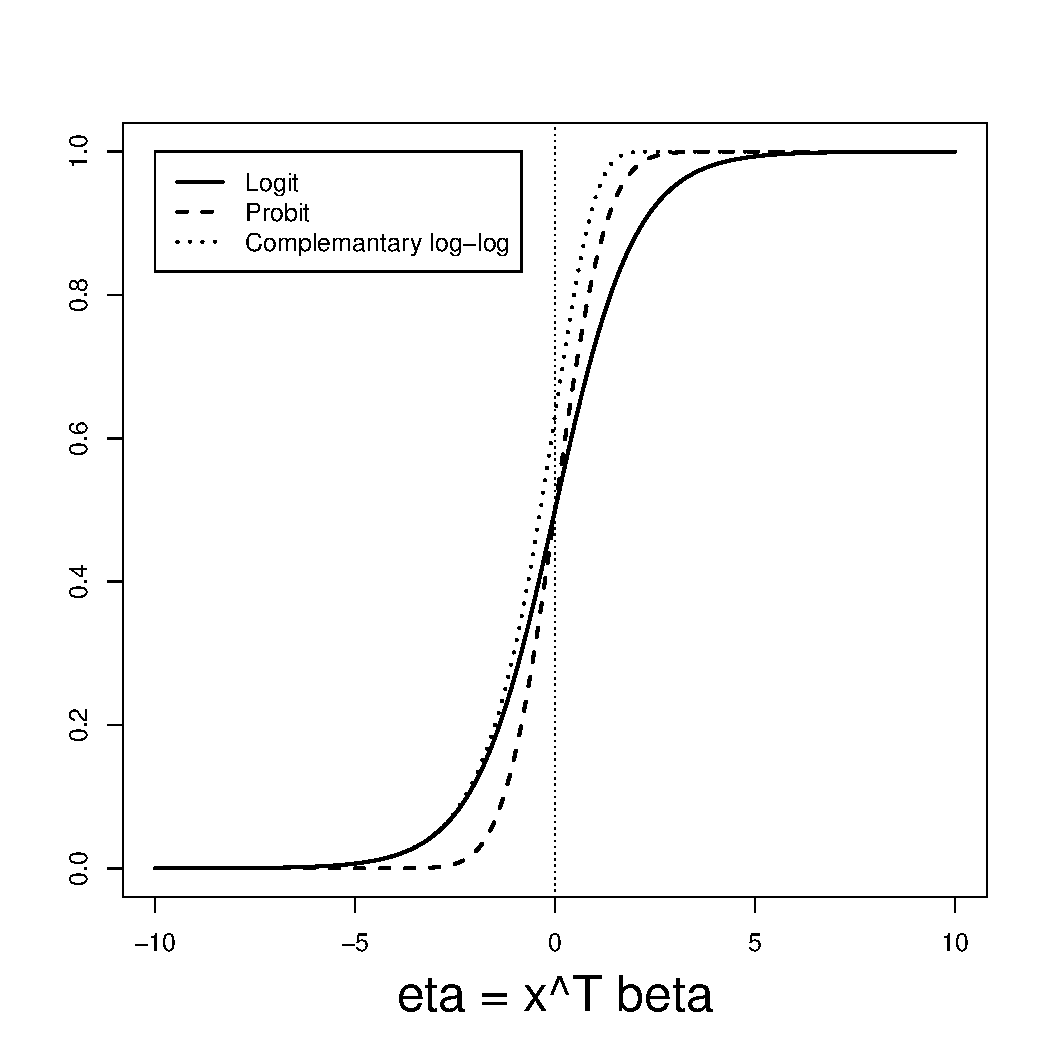
\includegraphics[width = 4.5cm]{figures/binarylinks.pdf}  
\end{center}

Which one? Difficult to test from data, because a large amount of
data is needed for small~$p$.

{\color{red} $\bigstar$ General families of link functions, see
\citeN{Aran:1981}}\\
 {\color{red}$\bigstar$ Nonparametric link for GLM, see \citeN{Weis:Wels:1994}}\\
{\color{red}$\bigstar$ Goodness of fit test for the link, see \citeN{Preg:1980}}
\end{frame}

\begin{frame}
\frametitle{}
The values  $o_i = \frac{p_i}{1-p_i}$ are called the odds. 

\bs

An odd of 2/3 means that there are 2 chances (out of 5) for success against 3
chances (out of 5) for failure.

\bs
Note: $p_i = \frac{o_i}{1+o_i}$.

\bs
The logit link has the advantage to allow interpretation on the odds scale.

\end{frame}


\begin{frame}
\frametitle{Poisson distribution: $Y_i \sim {\mathcal P}(\lambda_i)$}


Used to model count data, the number of occurrences of some event in a defined
time period or space. Examples: the number of medical conditions reported by a
person, the number of tropical cyclones during a season, the number of birds
observed on a particular day, the number of spelling mistakes on the page of a
newspaper, the number of incoming calls in 4 hours.

\bs
Here the link guarantees that $\lambda>0$. Common choices are:
$g(\mu_i) = g(\lambda_i) = \log(\lambda_i)$ (canonical link) or $g(\mu_i) =
\sqrt{\lambda}$. 

\end{frame}


\begin{frame}
\begin{center}
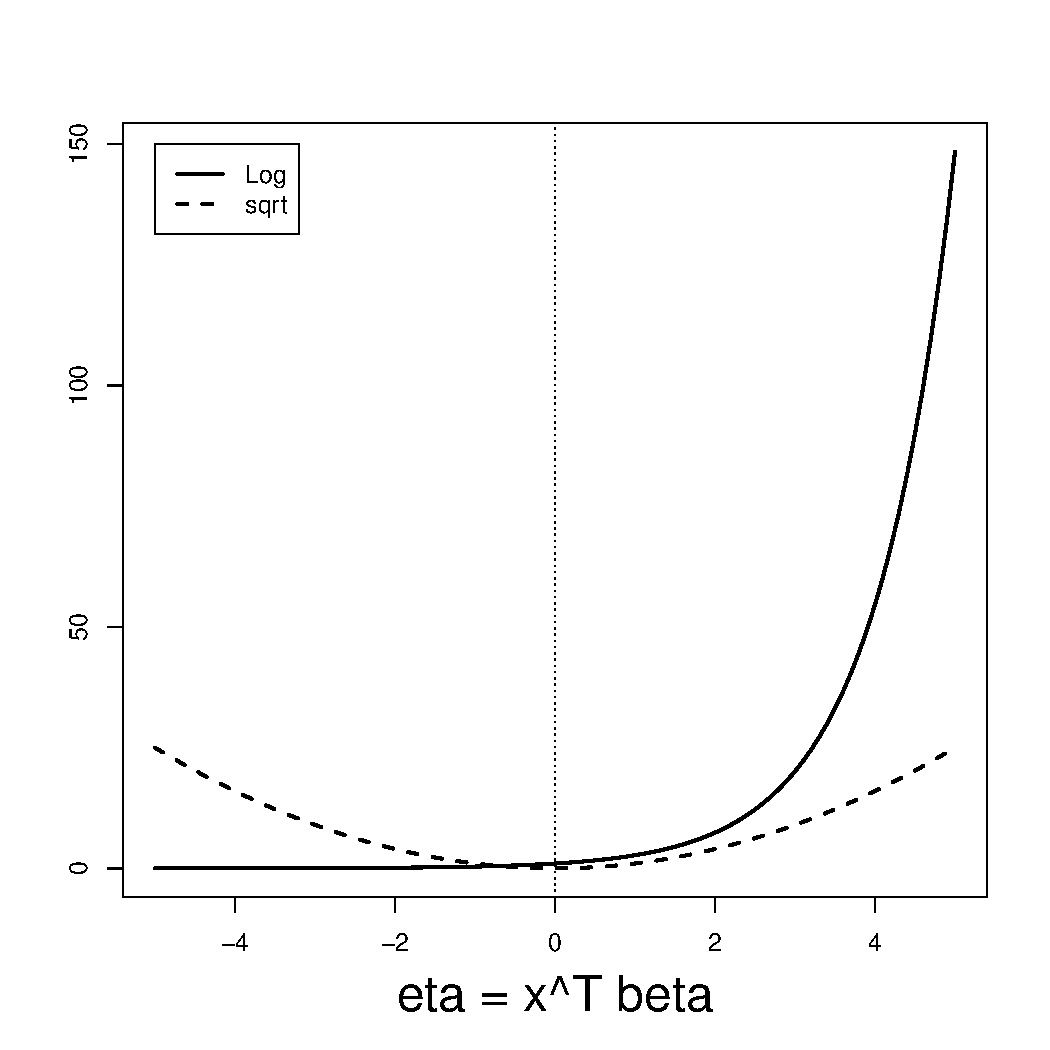
\includegraphics[width = 4.5cm]{figures/poissonlinks.pdf}  
\end{center}

\textbf{Remark}: the number of events out of a total is appropriately modelled by a
binomial distribution. But, if success probabilities are small and the totals
are large, the Poisson is a good approximation. (For small $p$,
$\mbox{logit}(p) = \log \left(\frac{p}{1-p} \right) \simeq \log(p)$.)
\end{frame}


\begin{frame}
\frametitle{Gamma distribution: $Y_i \sim \Gamma(\mu_i,\nu)$}

Used to model asymmetric continuous behaviors. For example, income or cost of
hospital stay.

\bs 
Here the link guarantees that $\mu_i>0$. A common choice is:
$g(\mu_i) = \log(\mu_i)$. The canonical link is $1/\mu_i$ but is more rarely
used. We note that the canonical link does not guarantee $\mu_i>0$.

\bs

\textbf{Remark}: the exponential distribution ${\mathcal E}(\lambda_i)$ is a
particular case where $\nu=1$.

\end{frame}


\begin{frame}
\frametitle{GLM Extensions}

In the spirit of GLM, some close models can be considered.

\bs

{\color{blue}Multinomial distribution:}

\bs
Generalization of the binomial distribution where there are $K$ possible
outcomes (instead of two), with associated probabilities $\pi_1, \ldots,
\pi_K$. Denote by $Y_i$ the random variable that takes values over categories
$1,\ldots,K$.


\bs
Need to distinguish between {\color{blue}nominal} data (no natural order) and 
{\color{blue}ordinal} data.
\end{frame}


\begin{frame}
\textbf{Nominal data}\\
Examples: eye color, party affiliation.

\bs
Denote by $Y_{ik}$ the number of observations falling into category $k$ for
individual $i$ (if only one measure, than only one of $Y_{i1},\ldots,Y_{iK}$ is
equal to one and the other are zero). Associated probabilities are $p_{ik} =
P(Y_i=k)$. 

\bs
Link the predictors $x_i$ to the probabilities through:
$$\log\left(\frac{p_{ik}}{p_{i1}} \right) = x_i^T \beta_k, \ \ \ k=2,\ldots,K$$
under the constraint that $\sum_{k=1}^K p_{ik}=1$, that is, $p_{i1}=1-
\sum_{k=2}^K p_{ik}$. 


\end{frame}


\begin{frame}
\frametitle{}

\textbf{Ordinal data}\\
Examples: food-testing, classification of radiographs, determination of physical and
mental well-being. 

\sms
The cumulative response probabilities 
$$\gamma_1 = \pi_1, \gamma_2=\pi_1+\pi_2, \ldots, \gamma_K=1,$$
that is $\gamma_k(x_i) = P(Y_i \leq k \mid x_i)$ are modelled. 

\bs
For example (logit-link model)
$$\log\left(\frac{\gamma_k(x_i)}{1-\gamma_k(x_i)} \right) = \alpha_k - x_i^T \beta$$
for $k=1, \ldots, (K-1)$. The negative sign on the linear predictor is a
convention ensuring that large values of $x_i^T \beta$ lead to an increase in
probability in the higher numbered categories.

\bs
\textbf{Extension}: allow for $\beta_k$ instead of $\beta$.
\end{frame}


\begin{frame}
\frametitle{}

This model is called the
{\color{blue}proportional-odds} model because the ratio of the event $Y \leq k$
at $x_i=x$ and $x_i = \tilde{x}$ is
$$\frac{\mbox{odds}(Y\leq k\mid x)}{\mbox{odds}(Y\leq k\mid
\tilde{x})} = \frac{\gamma_k(x)/(1-\gamma_k(x))}{\gamma_k(\tilde{x}) / 
(1-\gamma_k(\tilde{x}))} = \exp(-(x-\tilde{x})^T \beta),$$
independent of $\alpha_k$. In particular, if $x_i$ is an indicator for 2
treatments groups, $T_1$ and 
$T_2$, 
$$\frac{\mbox{odds}(Y\leq k \mid T_1)}{\mbox{odds}(Y\leq k\mid
T_2)}= \exp(-\Delta),$$
where $\Delta$ measures the treatment effect.

\sms
Alternatively one can use a complementary log-log link
$$ \log\left(-\log(1-\gamma_k(x_i))\right)= \alpha_k - x_i^T \beta,$$
which produces the {\color{blue}proportional hazard} model.

\bs
\textbf{Note}: in all of these models we need $\alpha_1 \leq \alpha_2 \leq
\ldots \leq \alpha_{K-1}$  to ensure that the probabilities are non-negative.
\end{frame}

\subsection{Parameters estimation}
\label{GLM.estim.section}

\begin{frame}[allowframebreaks]
\frametitle{Parameters estimation: maximum likelihood (ML)}
The likelihood function for the {\color{blue}canonical exponential 
family} is
\begin{eqnarray*}
  \label{lik.exp}
  \lefteqn{L(\theta_1,\ldots, \theta_n; y_1, \ldots, y_n)= \prod_{i=1}^n \exp \Big( A \ \frac{y_i \theta_i - b(\theta_i)}{\phi} +
c(y_i,\frac{\phi}{A})\Big) }\\
& = & \exp \Big( \frac{A}{\phi} \sum_{i=1}^n y_i \theta_i - \frac{A}{\phi}
\sum_{i=1}^n b(\theta_i) + \sum_{i=1}^n c(y_i,\frac{\phi}{A}) \Big)
\end{eqnarray*}
and the log-likelihood function is given by
$$l(\theta_1,\ldots, \theta_n; y_1, \ldots, y_n)
 =  \frac{A}{\phi} \sum_{i=1}^n y_i \theta_i - \frac{A}{\phi}
\sum_{i=1}^n b(\theta_i) + \sum_{i=1}^n c(y_i,\frac{\phi}{A}).$$

The relationship  $g(\mu_i) = x_i^T \beta$ is used in the above
likelihood function. Then the function is maximized with respect to
$\beta$ (by solving the score equations) to obtain $\hat{\beta}$.

\bs

No closed-form analytical expression for $\hat{\beta}$ is available in general.
\end{frame}

\begin{frame}
\frametitle{}

\textbf{Example}: if $Y_i$ is a binary response, that is, $Y_i \sim
Bernoulli(p_i)$, the likelihood is
\begin{equation*}
  \label{lik.bernoulli}
  L(p_1,\ldots, p_n; y_1, \ldots, y_n) = \prod_{i=1}^n p_i^{y_i} (1-p_i)^{1-y_i},
\end{equation*}
and the log-likelihood is

\begin{equation}
  \label{loglik.bernoulli}
l(p_1,\ldots, p_n; y_1, \ldots, y_n) = \sum_{i=1}^n y_i \log (p_i) + \sum_{i=1}^n (1-y_i) \log(1-p_i). 
\end{equation}

\bs
The logit link implies that $\log \big(\frac{p_i}{1-p_i}\big) = x_i^T
\beta$, and therefore that
$$p_i = \frac{\exp(x_i^T \beta)}{(1+\exp(x_i^T \beta))},$$
\end{frame}

\begin{frame}
\frametitle{}
which gives the log-likelihood
\begin{eqnarray*}
 \lefteqn{l(\beta;y)=l(\beta_0, \beta_1,\ldots,\beta_p; y_1, \ldots, y_n)=}\\
& = &  \sum_{i=1}^n y_i \log \Big(\frac{\exp(x_i^T \beta)}{1+\exp(x_i^T
  \beta)} \Big) +  \sum_{i=1}^n (1-y_i) \log\Big(\frac{1}{1+\exp(x_i^T \beta)} \Big) \\
& = &  \sum_{i=1}^n y_i x_i^T \beta -  \sum_{i=1}^n y_i \log( 1 +
\exp(x_i^T \beta)) \\
& & - \sum_{i=1}^n (1-y_i) \log(1+\exp(x_i^T \beta))\\
& = & \sum_{i=1}^n y_i x_i^T \beta - \sum_{i=1}^n \log(1+\exp(x_i^T \beta))
\end{eqnarray*}
\end{frame}

\begin{frame}
\frametitle{}

The score equations (differentiation with respect to $\beta$) are:
$$\sum_{i=1}^n \Big(y_i  - \frac{\exp(x_i^T \beta)}{1+\exp(x_i^T
  \beta)} \Big)   x_i = 0,$$
which have to be solved numerically.

\end{frame}

\subsection{Numerical methods}
\begin{frame}
\frametitle{Newton-Raphson procedure in the
univariate case}

For $x$ univariate, we would like to solve $h(x)=0.$

\bs

For small distances $x^{(m)} - x^{(m-1)}$, the slope is
\begin{equation}
  \label{NR.eq}
 h^{\prime}(x^{(m-1)}) = \frac{h(x^{(m)})-h(x^{(m-1)})}{x^{(m)} - x^{(m-1)}}.
\end{equation}

\bs
If $x^{(m)}$ is the required solution so that $h(x^{(m)})=0$, then
\eqref{NR.eq} can be rearranged to give
\begin{equation}
  \label{NRformula}
  x^{(m)} = x^{(m-1)} - \frac{h(x^{(m-1)})}{h^{\prime}(x^{(m-1)})}.
\end{equation}
This is the Newton-Raphson formula for solving $h(x)=0$ iteratively.
\label{Ufct}
\end{frame}

\begin{frame}
If we apply \eqref{NRformula} to maximize a log-likelihood $l(\beta;y)$, we
have
$$\beta^{(m)} = \beta^{(m-1)} - \frac{U^{(m-1)}}{U^{\prime (m-1)}},$$
where $U=  \frac{d l(\beta;y)}{d \beta}$.

\bs
For maximum likelihood estimation it is common to approximate
$U^{\prime}$ by $E(U^{\prime}) = - {\mathcal J}$ (the Fisher information), to obtain 
\begin{equation}
  \label{scoringformula}
  \beta^{(m)} = \beta^{(m-1)} + \frac{U^{(m-1)}}{{\mathcal J}^{(m-1)}}.
\end{equation}
This is called the {\color{blue}method of scoring}.
\end{frame}

\begin{frame}
\frametitle{}
The multivariate equivalents of  \eqref{NRformula} and
\eqref{scoringformula} are
$$\beta^{(m)} = \beta^{(m-1)} - \big[U^{\prime (m-1)}\big]^{-1} \ U^{(m-1)},$$
and respectively
\begin{equation}
  \label{multiscoring}
\beta^{(m)} = \beta^{(m-1)} + \big[{\mathcal J}^{(m-1)}\big]^{-1} \ U^{(m-1)},
\end{equation}
where $\beta$ and $U$ are now vectors of dimension $(p+1)$ and
${\mathcal J}$ is a $(p+1) \times (p+1)$ matrix.
\end{frame}

\subsection{IWLS algorithm for GLM}

\begin{frame}
\frametitle{ Iterative Weighted Least Squares (IWLS) algorithm}

Major steps of the {\color{blue} Iterative Weighted Least Squares (IWLS)}
algorithm for maximizing the log-likelihood for GLM (see \citeN{McCu:Neld:1989},
p.\ 40-42 for additional details) 

\bs
To solve:
$$\frac{\partial l(\beta;y)}{\partial \beta} =  \left(
\begin{array}{c}
\partial l(\beta;y)/\partial \beta_0\\
\vdots\\
\partial l(\beta;y)/\partial \beta_p
\end{array} \right) = 0$$

We have that
\begin{equation}
\label{scorej}
\frac{\partial l}{\partial \beta_j} = U_j = \sum_{i=1}^n
  \frac{\partial l_i}{\partial
  \beta_j} = \sum_{i=1}^n \frac{\partial l_i}{\partial \theta_i} \cdot
  \frac{\partial \theta_i}{\partial \mu_i} \cdot \frac{\partial
  \mu_i}{\partial \beta_j}.
\end{equation}
\end{frame}

\begin{frame}
\frametitle{}
First
$$\frac{\partial l_i}{\partial \theta_i} = A \frac{y_i -
b^{\prime}(\theta_i)}{\phi} \stackrel{\eqref{expect.exponential}}{=}
 A \frac{y_i-\mu_i}{\phi}.$$

\bs

Secondly $\frac{\partial \theta_i}{\partial \mu_i} = 1/(\frac{\partial
  \mu_i}{\partial \theta_i})$
and
$$\frac{\partial \mu_i}{\partial \theta_i}
\stackrel{\eqref{expect.exponential}}{=} b^{\prime \prime}(\theta_i)
\stackrel{\eqref{var.exponential}}{=} A \frac{Var(Y_i)}{\phi}$$

\bs
Finally
$$\frac{\partial \mu_i}{\partial \beta_j}=
\frac{\partial \mu_i}{\partial \eta_i} \cdot \frac{\partial
  \eta_i}{\partial\beta_j} = \frac{\partial \mu_i}{\partial \eta_i}
x_{ij}.$$

\bs

Putting everything together, \eqref{scorej} can be written as
$$\frac{\partial l}{\partial \beta_j} = U_j = \sum_{i=1}^n
\frac{y_i-\mu_i}{Var(Y_i)} x_{ij} \Big(\frac{\partial \mu_i}{\partial
  \eta_i}\Big)$$
\label{EE.GLM}
\end{frame}

\begin{frame}
We use the method of scoring (see~\eqref{multiscoring} on page~\pageref{multiscoring})  which implies
the computation of ${\mathcal J}$, whose
element $(j,k)$ is ${\mathcal J}_{jk} = E(U_j U_k)$ and is given by
\begin{eqnarray*}
  \lefteqn{{\mathcal J}_{jk} = E \left\{ \sum_{i=1}^n
\frac{y_i-\mu_i}{Var(Y_i)} x_{ij} \Big(\frac{\partial \mu_i}{\partial
  \eta_i}\Big) \cdot \sum_{l=1}^n
\frac{y_l-\mu_l}{Var(Y_l)} x_{lk} \Big(\frac{\partial \mu_l}{\partial
  \eta_l}\Big) \right\}} \hspace*{3cm}\\
& = & \ldots (\mbox{some extra computations})\\
& = &  \sum_{i=1}^n \frac{x_{ij} x_{ik}}{Var(Y_i)}
\Big(\frac{\partial \mu_i}{\partial
  \eta_i}\Big)^2
\end{eqnarray*}

${\mathcal J}$ can be written as $X^T W X$, where $W$ is a $n \times
n$ diagonal matrix with elements
$$w_{ii} = \frac{1}{Var(Y_i)} \Big(\frac{\partial \mu_i}{\partial
  \eta_i}\Big)^2$$
\end{frame}

\begin{frame}
The method of scoring is
$$\beta^{(m)} = \beta^{(m-1)} + \big[{\mathcal J}^{(m-1)}\big]^{-1} \ U^{(m-1)},  $$
and implies
$${\mathcal J}^{(m-1)} \beta^{(m)} = {\mathcal J}^{(m-1)}
\beta^{(m-1)} + U^{(m-1)}.$$

The right-hand side of the above can be written in our case
(computations omitted) as $X^T W^{(m-1)}
z^{(m-1)}$, where $z^{(m-1)}$ is a vector with elements
$$z_i^{(m-1)} = \sum_{k=0}^p x_{ik} \beta_k^{(m-1)} +
  (y_i-\mu_i^{(m-1)})\Big(\frac{\partial \eta_i}{\partial \mu_i}\Big)^{(m-1)},$$
where $\mu_i^{(m-1)}$ and $(\partial \mu_i/\partial \eta_i)^{(m-1)}$ are evaluated at
  $\beta^{(m-1)}$.
\end{frame}

\begin{frame}
Therefore the method of scoring amounts to solve with respect to $ \beta^{(m)}$
\begin{equation}
  \label{IWLS}
  X^T W^{(m-1)} X \beta^{(m)} = X^T W^{(m-1)} z^{(m-1)}.
\end{equation}
\label{IWLSweights}

\eqref{IWLS} is a weighted least squares problem to be solved
iteratively because ($z^{(m-1)}$ and $W^{(m-1)}$ depend on 
$\beta^{(m-1)}$). Only needs software that computes weighted least squares.

\bs
\textbf{Remarks}:
\begin{itemize}
\item $\frac{\partial \mu_i}{\partial \eta_i}$ depends on the link
  function used.
\item $Var(Y_i)$ depends on the model.
\item $\frac{\partial \mu_i}{\partial \eta_i}= b^{\prime \prime}(\theta) \propto Var(Y_i)$ when the canonical link
is used. This simplifies the estimating equations:
$\frac{\partial l}{\partial \beta_j} = U_j = \sum_{i=1}^n
(y_i-\mu_i) x_{ij}$
\end{itemize}
\end{frame}

\subsection{Breast cancer dataset}

\begin{frame}[fragile]
\frametitle{}

Consider the breast cancer dataset of Example~2
(p.~\pageref{example2}), and fit the simple model that explains the
outcome (\texttt{status}) as a function
of \texttt{nuclei} only (plus intercept) with a logit link.

\bs

{\scriptsize
\begin{lstlisting}
Call: glm(formula = status ~ nuclei, family = binomial, 
    data = breast,  na.action = na.omit)

Coefficients:
            Estimate Std. Error z value Pr(>|z|)    
(Intercept) -3.52218    0.23205  -15.18   <2e-16 ***
nuclei       0.85935    0.07092   12.12   <2e-16 ***
---
Signif. codes:  0 ‘***’ 0.001 ‘**’ 0.01 ‘*’ 0.05 ‘.’ 0.1 ‘ ’ 1

(Dispersion parameter for binomial family taken to be 1)

    Null deviance: 884.35  on 682  degrees of freedom
Residual deviance: 340.63  on 681  degrees of freedom
  (16 observations deleted due to missingness)
AIC: 344.63

Number of Fisher Scoring iterations: 6
\end{lstlisting}
}
\end{frame}

\begin{frame}
\frametitle{}
If $p_i = E(\texttt{status})$, the model is
$$\log\Big(\frac{p}{1-p}\Big) = \beta_0 + \beta_1 \texttt{nuclei}$$

\bs

\textbf{Interpretation}
\begin{itemize}
\item $\beta_1$ is related to the slope of the logistic curve (p.~\ref{slopelogit.fig}).
\item The effect of a unit change in \texttt{nuclei} is to increase log odds by
$\beta_1$. Equivalently, the effect of a unit change in  \texttt{nuclei} is to
increase the odds of a positive response multiplicatively by $\exp(\beta_1)$.
\item When more than one
covariate, same interpretation under the condition that the
other covariates are kept fixed.
\item The effect of a unit change in \texttt{nuclei} on $p_i$ is more
complicated to establish. In presence of several explanatory variables, this
effect would depend on the other covariates too.
\end{itemize}

\end{frame}

\begin{frame}
\frametitle{Logistic curves for different values of $\beta_1$}

\label{slopelogit.fig}
\begin{center}
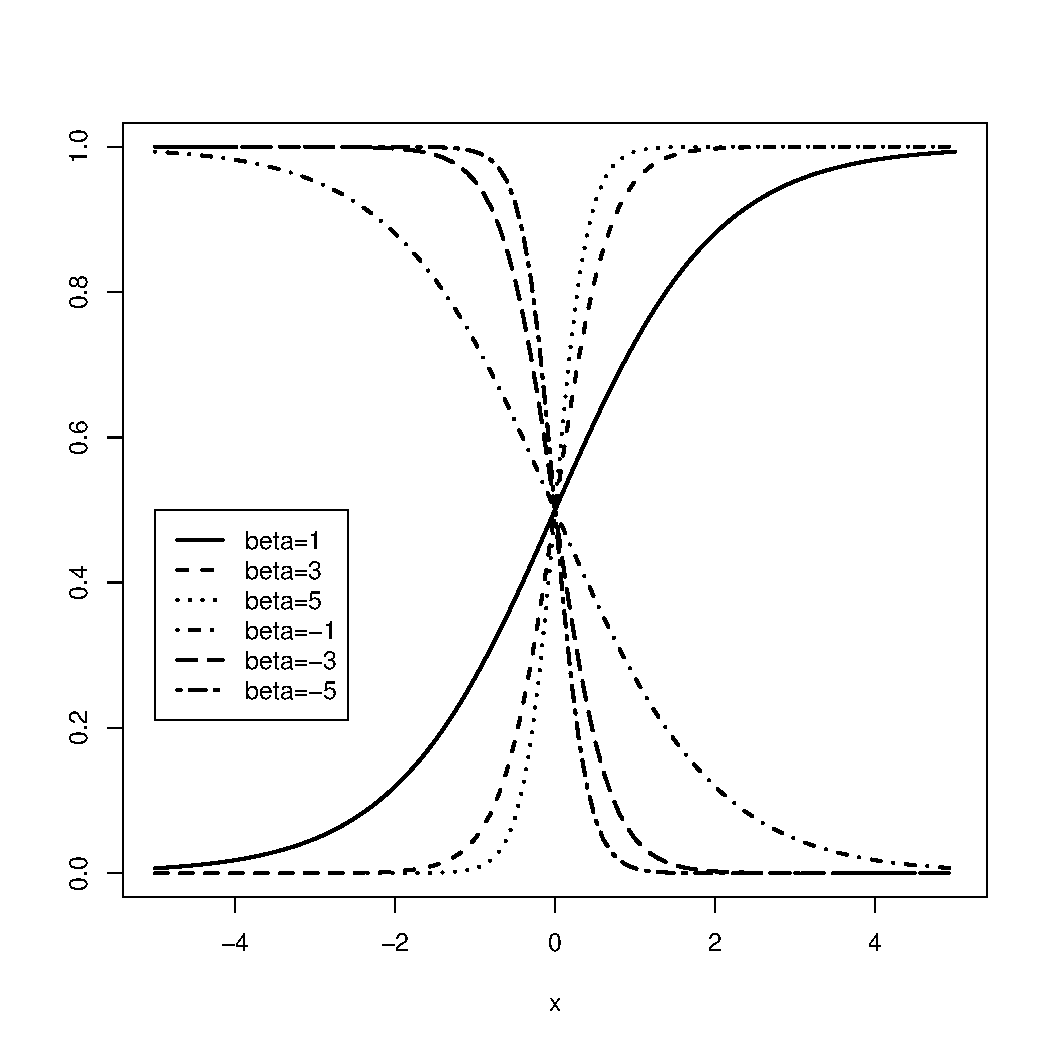
\includegraphics[width = 7.5cm]{figures/slopelogit.pdf}  
\end{center}

\end{frame}


\begin{frame}[fragile]
\frametitle{}
We can also fit the same model, but with a probit link.


\bs
{\scriptsize
\begin{lstlisting}
Call: glm(formula = status ~ nuclei, family = binomial(link = probit), 
    data = breast, na.action = na.omit)

Coefficients:
            Estimate Std. Error z value Pr(>|z|)    
(Intercept) -1.96960    0.10934  -18.01   <2e-16 ***
nuclei       0.45172    0.03177   14.22   <2e-16 ***
---
Signif. codes:  0 ‘***’ 0.001 ‘**’ 0.01 ‘*’ 0.05 ‘.’ 0.1 ‘ ’ 1

(Dispersion parameter for binomial family taken to be 1)

    Null deviance: 884.35  on 682  degrees of freedom
Residual deviance: 342.94  on 681  degrees of freedom
  (16 observations deleted due to missingness)
AIC: 346.94

Number of Fisher Scoring iterations: 7
\end{lstlisting}
}
\end{frame}


\begin{frame}
\frametitle{Logistic vs probit}

The parameter estimates of the probit model are quite different from those of the
logit model, because they don't have the same meaning:

$$\log\big(\frac{p_i}{1-p_i}\big) = x_i^T \beta^L \ \ \ \mbox{versus} \ \ \
\Phi^{-1}(p_i) = x_i^T \beta^P.$$

\bs

The fitted values (prediction for in-sample observations) are
obtained from the model formulation.
\end{frame}

\begin{frame}
\frametitle{}
For the logistic model, $\log(p_i/(1-p_i))
= x_i^T \beta^L$ implies $p_i = \exp(x_i^T \beta^L)/(1+\exp(x_i^T \beta^L))$ and
therefore
$$\hat{y_i} = \hat{p_i} =  \frac{\exp(x_i^T \hat{\beta}^L)}{(1+\exp(x_i^T
\hat{\beta}^L))}.$$

\bs
For the probit model, $\Phi^{-1}(p_i) = x_i^T \beta^P$ implies $p_i = \Phi(x_i^T
\beta^P)$ and therefore
$$ \hat{y_i} = \hat{p_i} = \Phi(x_i^T \hat{\beta}^P).$$
\end{frame}


\begin{frame}[fragile]
\frametitle{Fitted values with logit and probit model}

\begin{center}
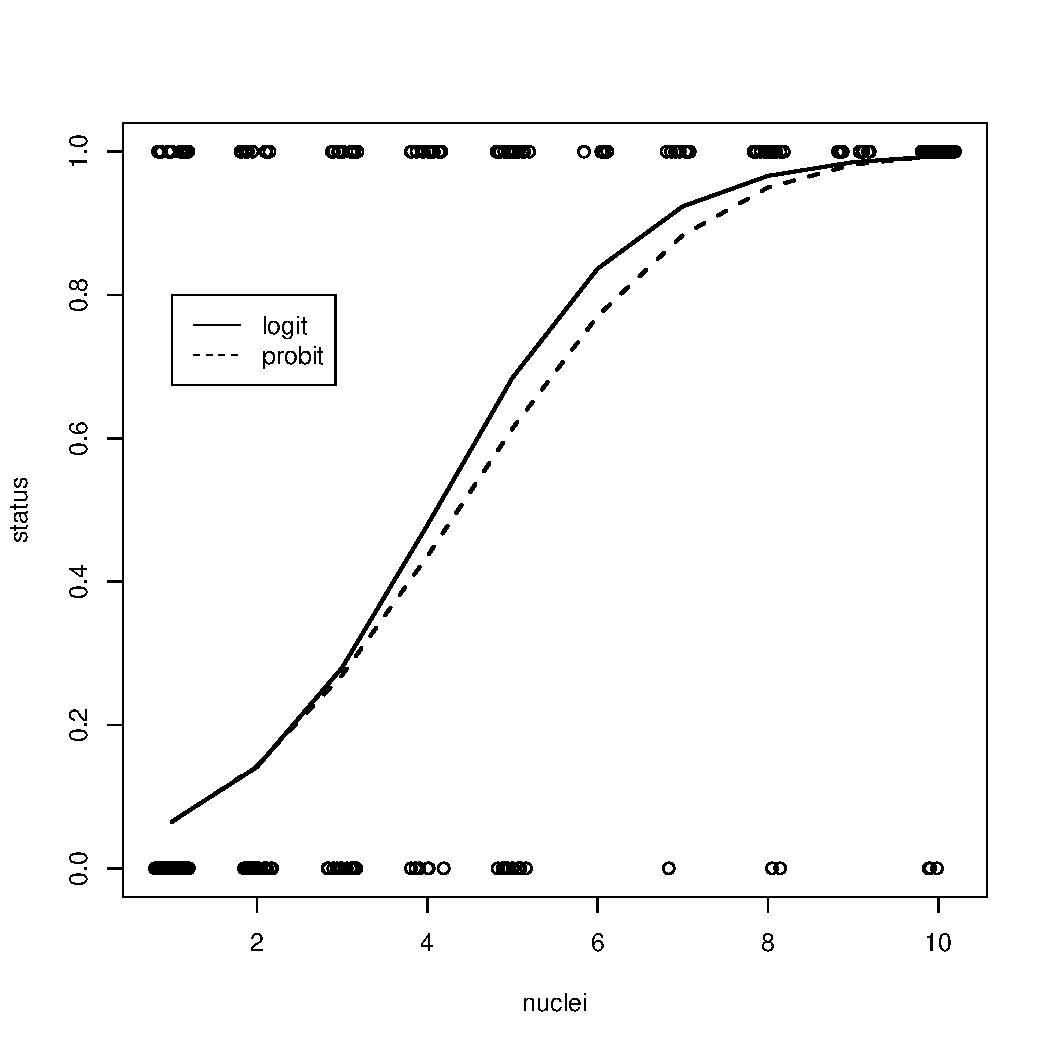
\includegraphics[width = 7cm]{figures/breastsub.pdf}  
\end{center}
\end{frame}


\subsection{Model checking}

\begin{frame}
\frametitle{Model validation}

\label{deviance.def}
One way of assessing the adequacy of a model is to compare it to a more general
model with the maximum number of parameters: a  {\color{blue}
saturated model}, which has the same number of parameters than
observations and leads to a perfect fit. The corresponding log-likelihood is 
denoted by $l(y;y)$.

\bs
The {\color{blue} scaled deviance} function is defined:
\begin{eqnarray*}
\lefteqn{D^*(y,\mu) = 2 \big[ l(y;y) - l(\hat{\beta};y) \big]=}\\
& = & \sum_{i=1}^n 2 \big[ l_i(y_i;y_i) - l_i(\hat{\beta};y_i) \big] =
\sum_{i=1}^n d_i,
\end{eqnarray*}
and the  {\color{blue} deviance} $D(y,\mu) = \phi D^*(y,\mu)$.
\label{deviance.comp}
\end{frame}

\begin{frame}
The deviance can be regarded as the likelihood ratio statistics for testing a
specific model within the saturated model, assuming $\phi=1$. 
This hypothesis is
true for binomial and Poisson models, for  which $D(y,\mu) =  D^*(y,\mu)$. For
other distributions, e.g. normal or Gamma, the deviance is not directly related
to a likelihood ratio statistic. 

\bs
Large values of $D$ indicate that the model is not good. On the other
hand, small values of $D$ (or $D^*$) arise when the log-likelihood $l(\beta;y)$
(from a model with $p$ parameters) is close to the log-likelihood
$l(y;y)$ (equivalent to a model with $n$ parameters).

\end{frame}


\begin{frame}
\frametitle{}
We have the following results:
\begin{itemize}
\item The distribution of $D^*$ is exactly
$\chi^2_{(n-(p+1))}$ if $Y_i$ is normally distributed ($D^*$ is the resid.\ 
sum of squares divided by $\sigma^2$). 
\item For certain other distributions of $Y_i$ the $\chi^2_{(n-(p+1))}$ can be taken
as an approximation for $D^*$.
\item $D$ (=$D^*$) is unusable when $Y_i$ is Bernoulli$(p_i)$. In this case, the
distribution of $D$ is degenerate (in fact, $D$ doesn't depend of $Y_i$).
\item The  $\chi^2_{(n-(p+1))}$ approximation works badly for $Y_i \sim {\mathcal
B}(m_i,p_i)$ if $m_i$ small (e.g. $<5$).
\item Except for the Bernoulli case, a bootstrap
  procedure could be
used to approximate the distribution of $D^*$.
\item In the case of Bernoulli, there is an ad-hoc fix, see {\color{red}
$\bigstar$ \citeN{Hosm:Leme:1980}}.
\end{itemize}
\end{frame}


\begin{frame}
\frametitle{}
An alternative goodness of fit statistic is the Pearson $X^2$ statistic:
$$X^2 = \sum_{i=1}^n \frac{(y_i - \hat{\mu}_i)^2}{v(\hat{\mu}_i)}.$$

\bs
The distribution of $X^2$ is $\chi^2_{n-(p+1)}$ for normally distributed $Y_i$ and
this approximation can be used for other distributions (see the discussion about
$D$).

\bs

It can be proven that $D$ and $X^2$ are related.
\end{frame}


\begin{frame}
\frametitle{Global measure of quality of the fit.}

\begin{itemize}
\item {\color{blue}Proportion of deviance explained}
$$(D_{null}-D)/D_{null},$$
where $D_{null}$ is the deviance of an intercept only fit.
\item An {\color{blue}extension of the $R^2$ measure} \cite{Nage:1991}:
\begin{eqnarray*}
\widetilde{R}^2 & = & \frac{1-(L_{null}/L)^{2/n}}{1-L_{null}^{2/n}}\\
\end{eqnarray*}
where $L_{null}$ is the likelihood of an intercept only fit.
\end{itemize}
\end{frame}

\begin{frame}
\frametitle{Residual analysis}

Several type of residuals can defined for GLM models. In particular, 
\begin{itemize}
\item {\color{blue}Pearson residuals}: $r_{iP} = \frac{y_i - \hat{\mu}_i}{\sqrt{v(\hat{\mu}_i)}},$
\item {\color{blue}deviance residuals}: $r_{iD} = \mbox{sign}(y_i - \hat{\mu_i}) \sqrt{d_i},$
where $d_i$ are the individual deviance components to $D$ (see page~\pageref{deviance.comp}).
\item {\color{blue}deviance standardized residuals}: $r_{iDS} = \frac{r_{iD}}{\sqrt{1-h_{ii}}},$
where $h_{ii}$ are the diagonal elements of the hat matrix $H=X(X^T
X)^{-1}X^T$.
\end{itemize}

\bs
\textbf{Note}: \\
$\sum_{i=1}^n r_{iP}^2 = X^2$ and $\sum_{i=1}^n r_{iD}^2 =
\sum_{i=1}^n d_i = D$.

\end{frame}

\begin{frame}
\frametitle{}
Residuals are usually plotted:
\begin{itemize}
\item against the fitted values to check for lack of fit (departures/structure).
\item against the normal quantiles (QQ-plot). 
\item in the order of measurements to check for serial correlation.
\item against each continuous explanatory variable to check the linearity
assumption.
\end{itemize}

\bs
\textbf{Remarks}: 
\begin{itemize}
\item Structures very often appears for $Y_i \sim {\mathcal B}(m_i,p_i)$ for small values of $m_i$.
\item Factors in the covariates can induce particular structures in the residuals.
\end{itemize}

\bs
\textbf{Note}: 
Normality of the residuals is not expected, and therefore the normal
QQ-plot have to be interpreted with caution.
\end{frame}

\begin{frame}
\frametitle{}
Illustration with simulated data from the model 
$$Y_i \sim Bernoulli(p_i),$$
with $p_i = \exp(x_i^T \beta) /(1+ \exp(x_i^T \beta))$, where $x_i^T = (1, z_i)$ with $z_i \sim N(0,1)$ and $\beta^T = (1, 0.5)$.

\begin{center}
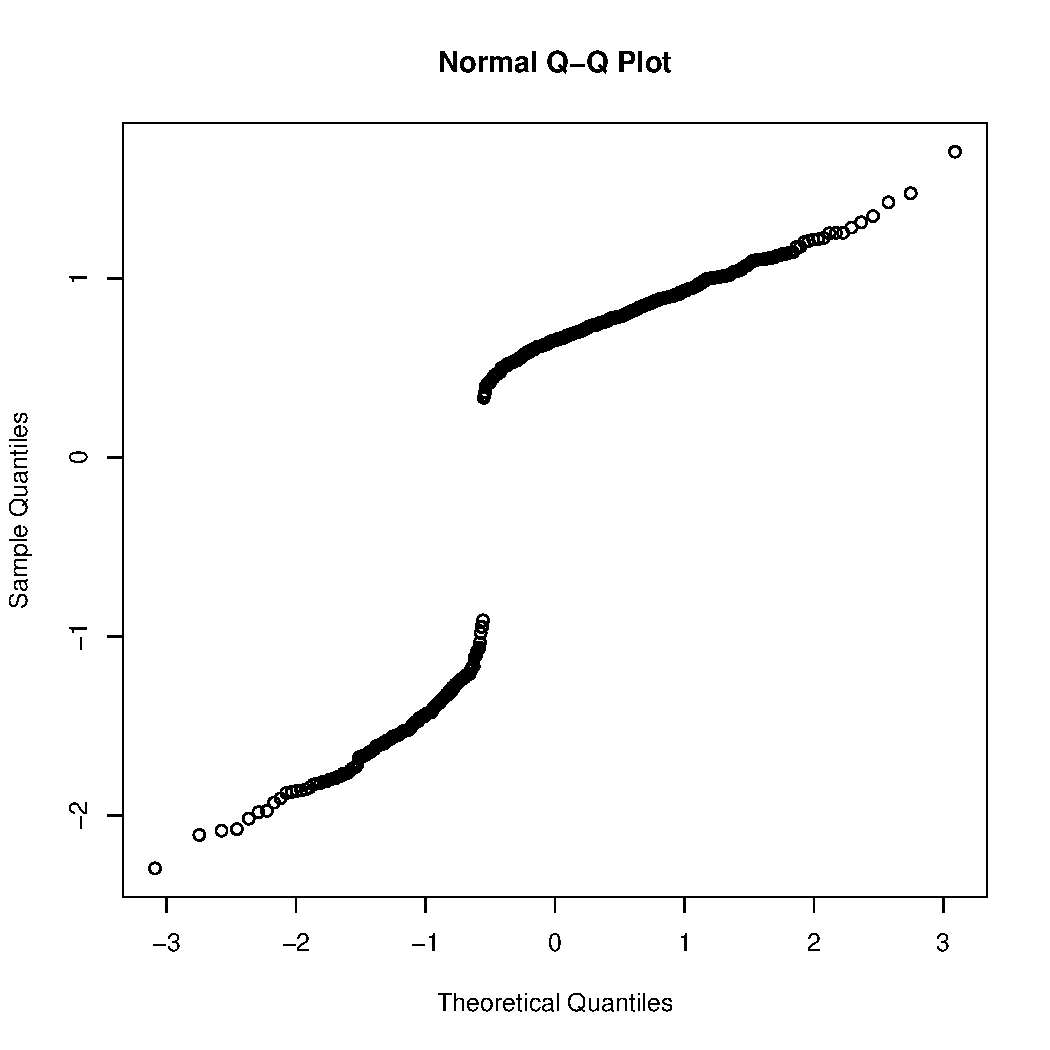
\includegraphics[width = 5.5cm]{figures/QQnormBernoulliSim.pdf}  
\end{center}

\end{frame}

\begin{frame}
\frametitle{Alternative: randomized quantile residuals}

Let $F = F_{\theta_i}$ be the cumulative distribution function of $Y_i$ and
$\Phi$ be the cumulative distribution function of a standard normal random
variable.

\sms
The ``randomized quantile residuals'' are defined by:
\begin{itemize}
\item if $F$ is continuous: $r_{iQ} = \Phi^{-1}(F(y_i; \hat{\mu}_i,\hat{\phi}))$. 
\item if $F$ is discrete: $r_{iQ} = \Phi^{-1}(u_i)$, with $u_i$ a uniform random variable on the
interval $(a_i,b_i]$, with $a_i = \lim_{y \rightarrow y_i} F(y;
\hat{\mu}_i,\hat{\phi})$ and $b_i=F(y_i; \hat{\mu}_i,\hat{\phi})$, 
\end{itemize}

The distribution of the ``randomized quantile residuals'' is exactly standard
normal, apart from sampling variability in $\hat{\mu}_i$ and $ \hat{\phi}$ (thanks to the probability integral transform).

\sms
Note: When $Y_i$ is discrete, the definition includes a randomization step: useful to look at several realizations.
\end{frame}


\begin{frame}[fragile]
\frametitle{}
On the previous simulated logistic example:

\begin{center}
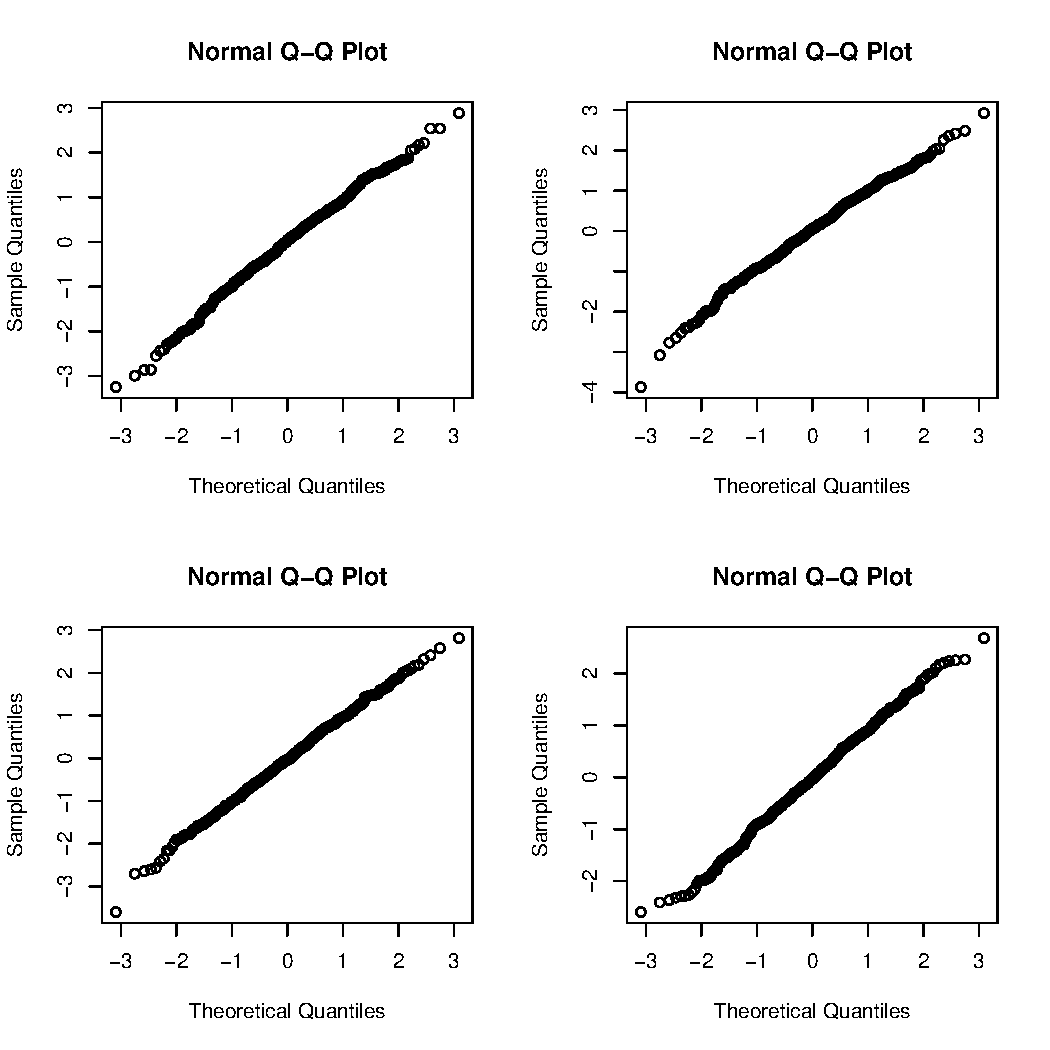
\includegraphics[width = 5.5cm]{figures/QQrandomizedBernoulliSim.pdf}  
\end{center}

{\scriptsize
\begin{lstlisting}
> require(statmod) 
> qqnorm(qresid(glm.sim))
\end{lstlisting}
}
\end{frame}

\subsection{Example 4: Gamma}

\begin{frame}[fragile]
\frametitle{Example 4 of page~\pageref{CHUV.Ex}} 
\label{Routput.gamma}


\bs 
{\tiny
\begin{lstlisting}
Call: glm(formula = CouTot ~ log(LOS) + Typadm + Typass + age + Sexe + 
    dest, family = Gamma(link = log), data = MYdata)

Coefficients:
              Estimate Std. Error t value Pr(>|t|)    
(Intercept)  7.2338121  0.1468364  49.264  < 2e-16 ***
log(LOS)     0.8222203  0.0279641  29.403  < 2e-16 ***
Typadm       0.2136148  0.0500028   4.272 4.67e-05 ***
Typass       0.0932763  0.0791100   1.179   0.2414    
age         -0.0005335  0.0012852  -0.415   0.6790    
Sexe         0.0951009  0.0499814   1.903   0.0602 .  
dest        -0.1043560  0.0692713  -1.506   0.1353    
---
Signif. codes:  0 ‘***’ 0.001 ‘**’ 0.01 ‘*’ 0.05 ‘.’ 0.1 ‘ ’ 1

(Dispersion parameter for Gamma family taken to be 0.04961642)

    Null deviance: 47.9536  on 99  degrees of freedom
Residual deviance:  5.0718  on 93  degrees of freedom
AIC: 1817.9

Number of Fisher Scoring iterations: 5
\end{lstlisting}
}
\end{frame}


\begin{frame}
\frametitle{}
The deviance is $D=5.07$ in this example see \texttt{Residual
  Deviance} in \texttt{summary(MYglm)}.

\bs
We use it to test the hypothesis $H_0$ that our model fits the data well.

\bs
The p-value is $P(D > 5.07)$, which has to be computed according to a
$\chi^2_{93}$ distribution. This probability is very close to 1, providing no
evidence against $H_0$.

\end{frame}

\begin{frame}[fragile]
\frametitle{Pearson and deviance residuals}

\begin{center}
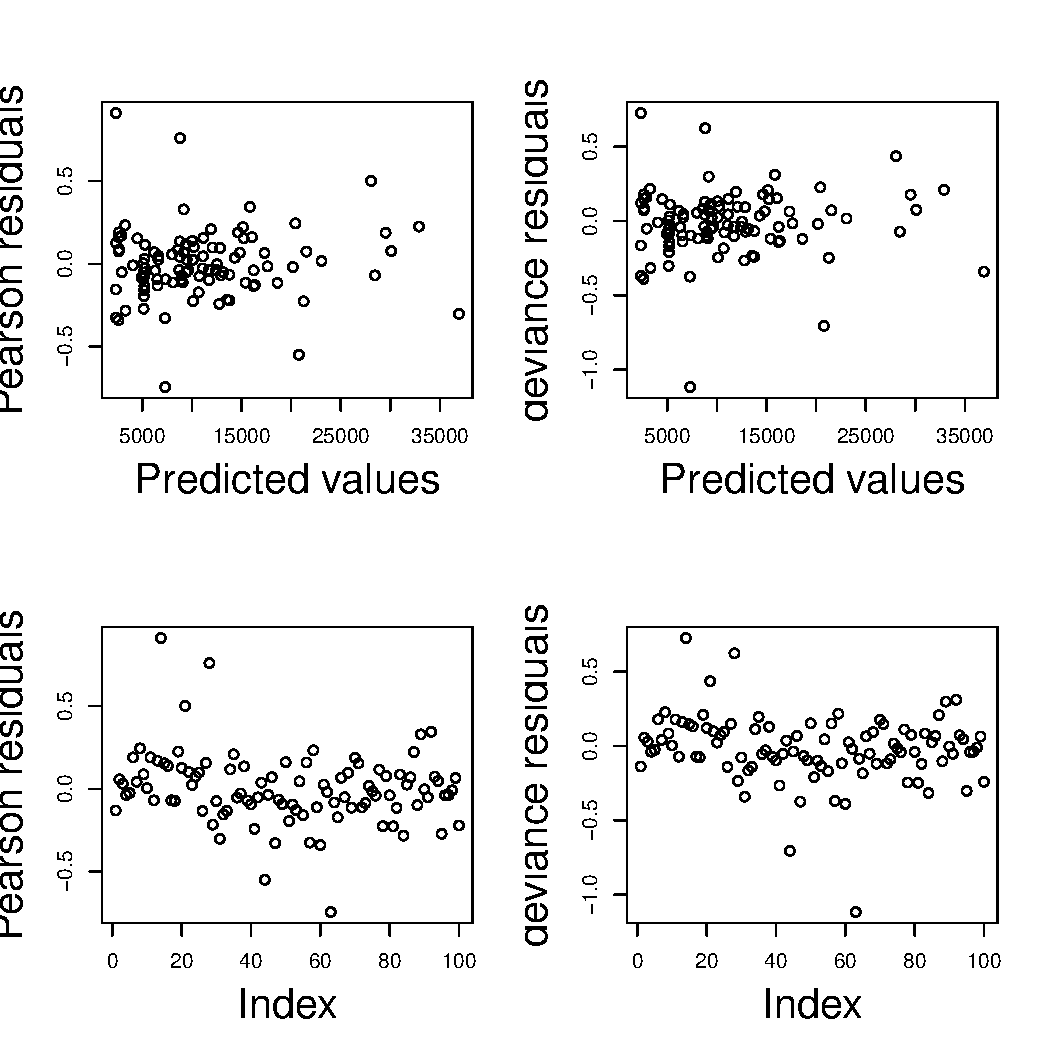
\includegraphics[width = 7cm]{figures/MYresid.pdf}  
\end{center}
\end{frame}



\begin{frame}
\frametitle{Pearson residuals against continuous covariates}
\begin{center}
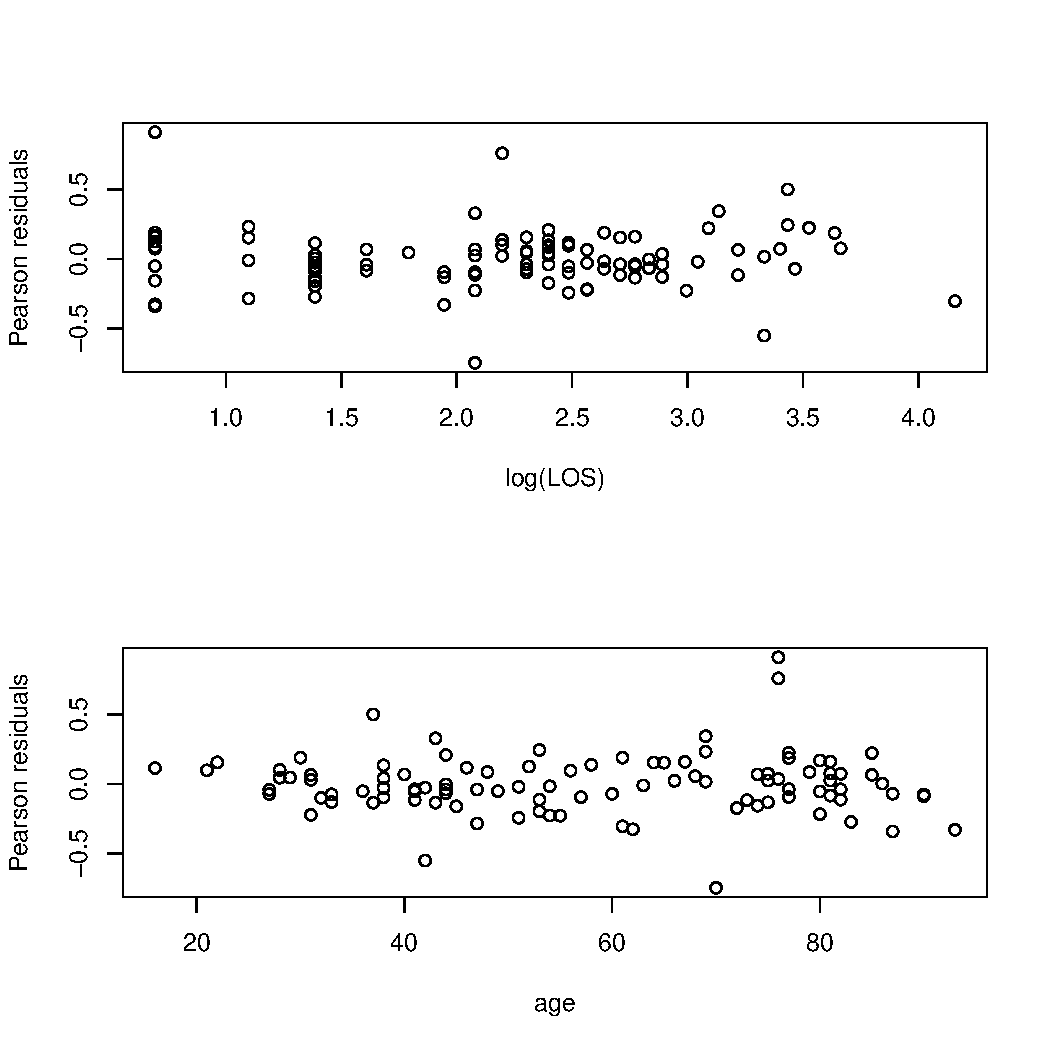
\includegraphics[width = 7cm]{figures/MYresid1.pdf}  
\end{center}
\end{frame}



\begin{frame}
\frametitle{}

\begin{center}
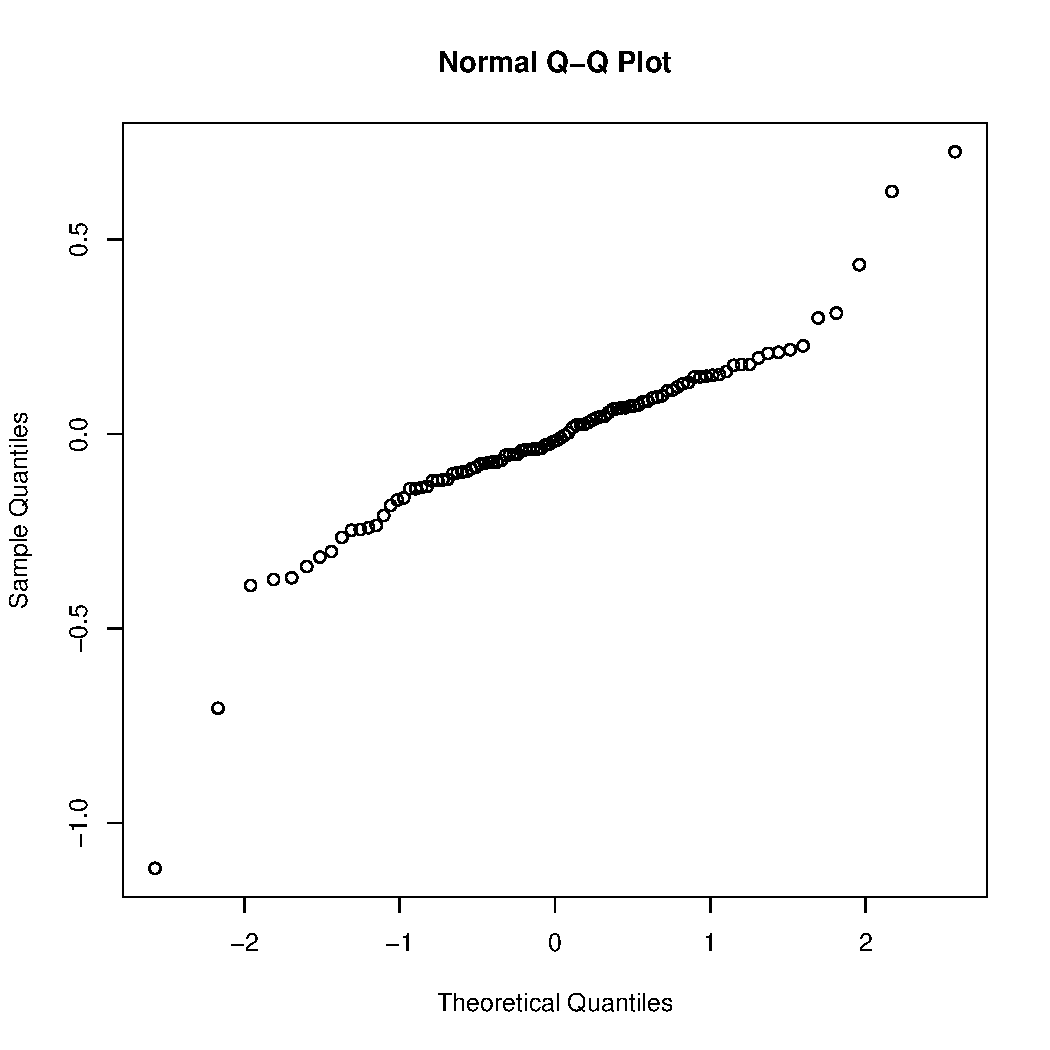
\includegraphics[width = 5.5cm]{figures/QQresid.pdf}  
\end{center}

\textbf{Note}:  $\texttt{plot()}$ in R produces
similar plots, plus the Cook distances plot that allows to identify
influential observations.
\end{frame}



\begin{frame}
\frametitle{}
\begin{center}
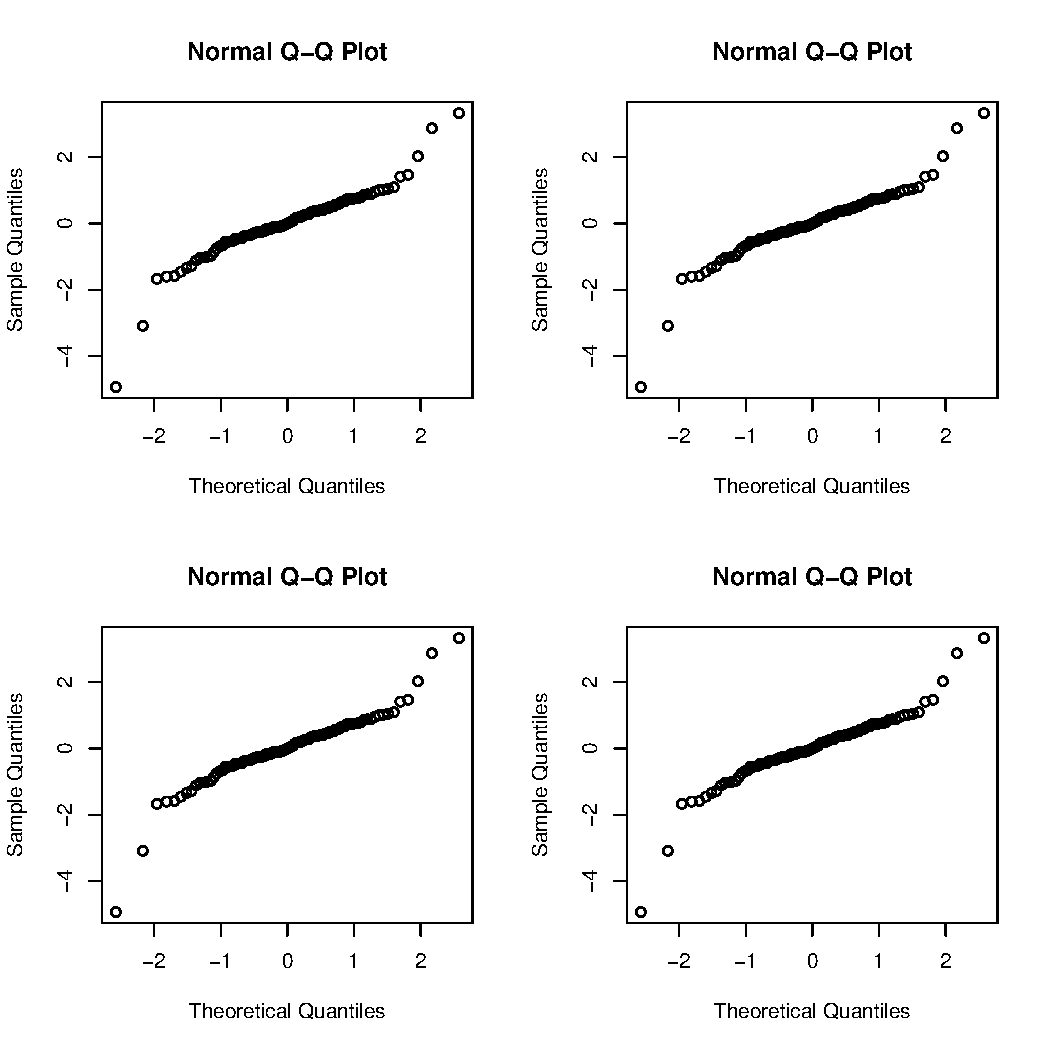
\includegraphics[width = 5cm]{figures/QQresidQrandom.pdf}  
\end{center}

The plots are the same! (no randomization involved).

\bs
There seem to be a few outliers, this dataset will be reanalyzed in
Chapter~\ref{robust.section}.
\end{frame}

\subsection{Confidence intervals and z-tests}
\begin{frame}
\frametitle{Confidence intervals}
The estimator of $\beta$ in a GLM is usually obtained by maximum
likelihood. This means that $\hat{\beta}$ inherits of the general
maximum likelihood properties, in particular the asymptotic
distribution. Based on
$$ (\hat{\beta}- \beta) \sim {\mathcal N} (0,\tilde{\mathcal J}^{-1}), $$
where $\tilde{J}$ is the information matrix computed from the joint likelihood, the computation of an asymptotic
approximation to the standard error of $\hat{\beta}$ is possible.
\end{frame}


\begin{frame}
\frametitle{}
From the asymptotic normality result, it follows that $(1-\alpha)$-confidence
intervals for each parameter can be constructed as: 
$$\big[\hat{\beta}_i - z_{1-\alpha/2} \sqrt{(\tilde{\mathcal J}^{-1})_{ii}} ;\hat{\beta}_i +
z_{1-\alpha/2} \sqrt{(\tilde{\mathcal J}^{-1})_{ii}} \big],$$
where $z_{1-\alpha/2}$ is the $(1-\alpha/2)$-quantile of a ${\mathcal
  N}(0,1)$-distribution.

\bs
These intervals are symmetric by construction.

\bs
These con\-fi\-den\-ce intervals may work poorly, in particular if the distribution of the parameter 
estimator is markedly skewed. 
\end{frame}


\begin{frame}
\frametitle{}
In contrast, {\color{blue}profiled likelihood confidence intervals} don't assume
normality of the estimator and perform better for small sample sizes. They are
obtained by inverting the likelihood  ratio statistics, and as such they are
still based on asymptotic approximation (the $\chi^2$ distribution of the
log-likelihood ratio statistic). 

\bs
For a model with parameter $\theta$ of interest and $\delta$ (extra parameters),
the profile likelihood is 
$$L_1(\theta) = \max_{\delta} L(\theta,\delta).$$
\end{frame}


\begin{frame}
\frametitle{}
A $(1-\alpha)$ profiled likelihood confidence intervals is the set of all values
$\theta_0$ such that a two-sided test of the null hypothesis $H_0: \theta =
\theta_0$ would not be rejected at the $\alpha$ level. The likelihood ratio test
statistic is used.

\bs
These confidence intervals are not symmetric, although the result is usually
close to the confidence intervals obtained from the maximum likelihood theory.
\end{frame}


\begin{frame}
\frametitle{}
\textbf{z-values} for testing ($H_0: \beta_i=0$ against $H_A: \beta_i \neq
0$), which  correspond to a test on the variable $x_i$:
$$\texttt{z-value} = \frac{\hat{\beta}_i}{s.e.(\hat{\beta}_i)} =
\frac{\hat{\beta}_i}{\sqrt{({\mathcal J}^{-1})_{ii}}} \stackrel{H_0}{\sim} {\mathcal
  N}(0,1).$$
Then compute the p-value
\begin{eqnarray*}
\lefteqn{P(|\texttt{z-value}| > |z_{obs}|) = \hspace*{3cm}}\\
& = & P(\texttt{z-value} < - |z_{obs}|) + P(\texttt{z-value} > |z_{obs}|) =\\
& = & 2 (1-P(\texttt{z-value} > |z_{obs}|)) =2 ( 1 - \Phi^{-1}(|z_{obs}|)).
\end{eqnarray*}

\bs
\textbf{Note:} If the distribution depends also on a nuisance or extra
parameter (normal, Gamma), the $t_{n-(p+1)}$ distribution is used instead of the
normal distribution as reference distribution of the \texttt{z}-statistic under $H_0$. The \texttt{z-values} are called
\texttt{t-values} in this case, see for example the output of the Gamma example
on page~\pageref{Routput.gamma}.
\end{frame}

\subsection{Hypothesis testing}
\begin{frame}
\frametitle{Hypothesis testing}
To test a parametric hypothesis on $\beta$, e.g. $H_0:
\beta=\tilde{\beta}$, the three classical tests are available:

\begin{description}
\item[Wald statistic] $(\hat{\beta} -\tilde{\beta})^T {\mathcal J}(\tilde{\beta})
  (\hat{\beta} -\tilde{\beta})$ which follows a $\chi^2_{p+1}$
  distribution under $H_0$.
\item[score statistic] $U(\tilde{\beta})^T {\mathcal
J(\tilde{\beta})}^{-1}U(\tilde{\beta})$ which follows a 
  $\chi^2_{p+1}$ distribution under $H_0$, ($U$ is the score function defined on
  page~\pageref{Ufct}).
\item[likelihood-ratio statistic] $2
  [l(\hat{\beta};y)-l(\tilde{\beta};y)]$ which is in fact a difference
  of deviances, see below.
\end{description}
\end{frame}

\subsection{Variable selection}
\begin{frame}
\frametitle{Variable selection}

Compare two models: a ${\mathcal M}_{p+1}$ with $(p+1)$
parameters and a {\color{blue} nested} model ${\mathcal M}_{p+1-q}$
with $(p+1-q)$ parameters (that is a model that contains a subset of the
variables in ${\mathcal M}_{p+1}$).

\bs
Common practice in GLM is to use difference of deviances for
variable (model) selection.

\bs
To test the null hypothesis
$$H_0: \beta = (\cdot, \ldots, \cdot, 0_{p+2-q},\ldots,0_{p+1})$$
(the model with $(p+1-q)$ parameters is enough), we
define the difference of scaled deviances
\begin{eqnarray*}
  \lefteqn{\Delta D^* = D^*(y,\hat{\mu}^{p+1-q}) - D^*(y,\hat{\mu}^{p+1}) = }\\ 
& = & 2 \Big[ l(\hat{\beta}^{p+1};y) - l(\hat{\beta}^{p+1-q};y)\Big] = \frac{D(y,\hat{\mu}^{p+1-q}) - D(y,\hat{\mu}^{p+1})}{\phi}
\end{eqnarray*}

\end{frame}



\begin{frame}
\frametitle{}
If $\phi$ is known and under $H_0$, the asymptotic distribution of $\Delta D^*$ is
$\chi^2_{q}$ (it is the likelihood ratio statistics). This approximation 
is much better than the approximation of the deviance itself. 

\bs
When $\phi$ is not known (e.g.\ Normal, Gamma, ``quasi'' type of models) the
usual approximation under 
$H_0$ uses an $F$ statistic:
$$\frac{(D(y,\hat{\mu}^{p+1-q}) - D(y,\hat{\mu}^{p+1}))/q}{\hat{\phi}} \sim
F_{q,n-(p+1)},$$
where $\hat{\phi}= \frac{D(y,\hat{\mu}^{p+1})}{n-(p+1)}$. 

\bs
Note that for the normal-identity case this is an exact result, but for the
Gamma the accuracy of this approximation is not well known.
\end{frame}

\begin{frame}
\frametitle{}
The difference of deviances is often used in a sequential approach, either
forward (starting from the null/constant model) or backward (starting
from the full model).

\bs
{\color{blue}Drawback} of this approach: the final model depends on
the (a priori) arbitrary ``path'' of the procedure.
\end{frame}


\begin{frame}
\frametitle{}
A full approach would be to use a general criterion to compare all
possible models. One of such criteria is the {\color{blue}Akaike information
criterion (AIC)}, which for a general model ${\mathcal M}_{d}$ with $d$
parameters is defined by:
\begin{eqnarray*}
\lefteqn{-2 l(\hat{\beta}^d;y) + 2d  \varpropto   D^*(y,\hat{\beta}^d) + 2d} \\
& = & \frac{D(y,\hat{\beta}^d)}{\phi} + 2 d \varpropto  D(y,\hat{\beta}^d) + 2 \phi d.
\end{eqnarray*}
Need to estimate $\phi$.

\bs
This criterion takes into account the complexity of the model
(measured by the number of parameters).
Models with low AIC have to be preferred.

\bs
Not feasible to compare all possible models for large $p$ ($2^p$
models). Use stepwise AIC.
\end{frame}


\subsection{Breast cancer dataset}
\begin{frame}[fragile]
\frametitle{Breast cancer dataset}
{\tiny
\begin{lstlisting}
Coefficients:
             Estimate Std. Error z value Pr(>|z|)    
(Intercept) -10.10394    1.17488  -8.600  < 2e-16 ***
clump         0.53501    0.14202   3.767 0.000165 ***
cellsize     -0.00628    0.20908  -0.030 0.976039    
cellshape     0.32271    0.23060   1.399 0.161688    
adhesion      0.33064    0.12345   2.678 0.007400 ** 
singlesize    0.09663    0.15659   0.617 0.537159    
nuclei        0.38303    0.09384   4.082 4.47e-05 ***
chromatin     0.44719    0.17138   2.609 0.009073 ** 
nucleoli      0.21303    0.11287   1.887 0.059115 .  
mitoses       0.53484    0.32877   1.627 0.103788    
---
Signif. codes:  0 ‘***’ 0.001 ‘**’ 0.01 ‘*’ 0.05 ‘.’ 0.1 ‘ ’ 1

(Dispersion parameter for binomial family taken to be 1)

    Null deviance: 884.35  on 682  degrees of freedom
Residual deviance: 102.89  on 673  degrees of freedom
  (16 observations deleted due to missingness)
AIC: 122.89

Number of Fisher Scoring iterations: 8
\end{lstlisting}
}
\end{frame}


\begin{frame}
\frametitle{Randomized residuals}
\begin{center}
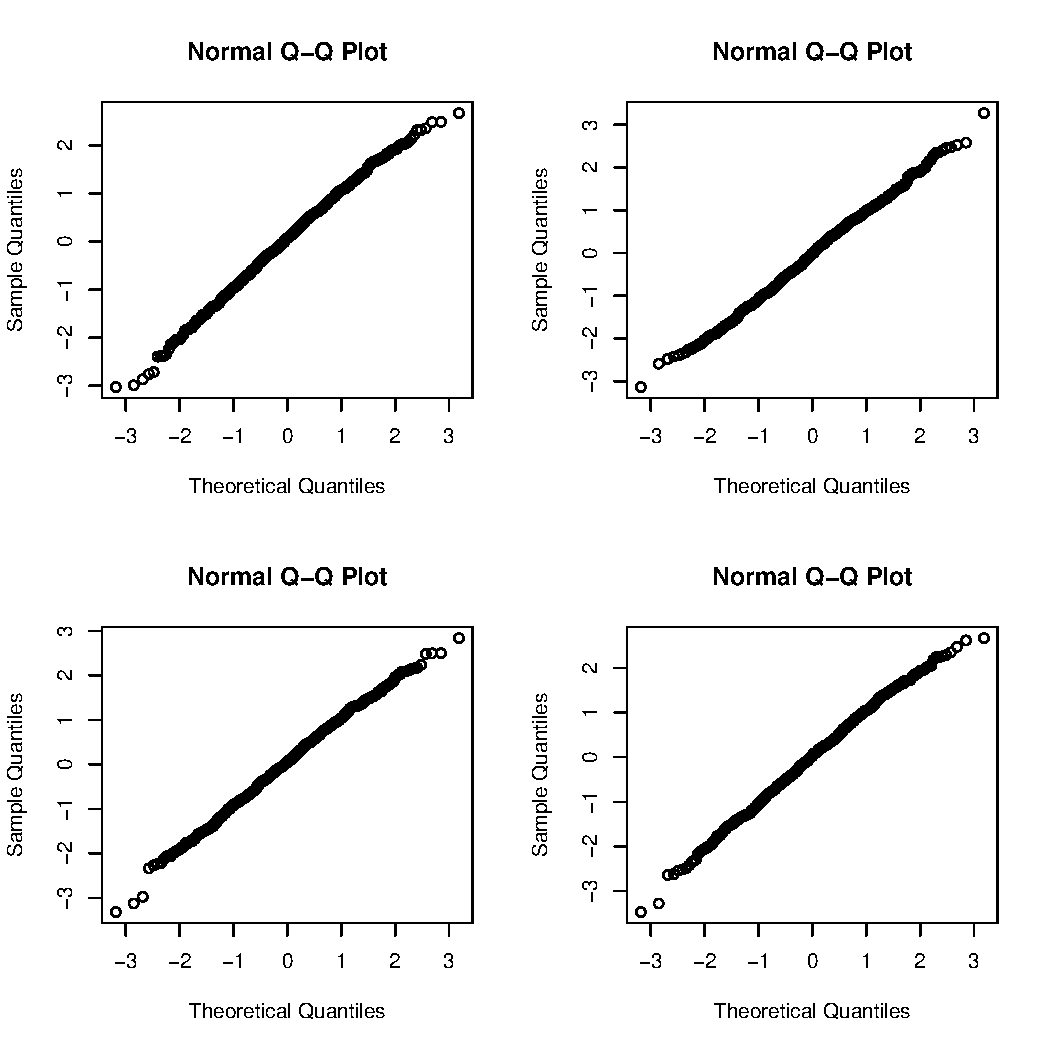
\includegraphics[width = 7cm]{figures/breastQQrandom.pdf}  
\end{center}
\end{frame}


\begin{frame}[fragile]
\frametitle{}
Profiled $95\%$ confidence intervals:

{\tiny
\begin{lstlisting}
> round(confint(breast.fit,level=0.95),4)
Waiting for profiling to be done...
               2.5 %  97.5 %
(Intercept) -12.7581 -8.0851
clump         0.2742  0.8377
cellsize     -0.3948  0.4379
cellshape    -0.1482  0.7684
adhesion      0.0930  0.5869
singlesize   -0.2169  0.4049
nuclei        0.2069  0.5787
chromatin     0.1232  0.7998
nucleoli     -0.0018  0.4456
mitoses      -0.0067  1.1065
\end{lstlisting}
}

and  $95\%$ confidence intervals based on asymptotic normality:
{\tiny
\begin{lstlisting}
> round(confint.default(breast.fit,level=0.95),4)
               2.5 %  97.5 %
(Intercept) -12.4067 -7.8012
clump         0.2567  0.8134
cellsize     -0.4161  0.4035
cellshape    -0.1293  0.7747
adhesion      0.0887  0.5726
singlesize   -0.2103  0.4036
nuclei        0.1991  0.5670
chromatin     0.1113  0.7831
nucleoli     -0.0082  0.4343
mitoses      -0.1095  1.1792
\end{lstlisting}
}
\end{frame}


\begin{frame}[fragile]
\frametitle{Analysis of deviance (sequential):}

{\tiny
\begin{lstlisting}
> anova(breast.fit,test="Chisq")

Terms added sequentially (first to last)

           Df Deviance Resid. Df Resid. Dev  Pr(>Chi)    
NULL                         682     884.35              
clump       1   425.87       681     458.48 < 2.2e-16 ***
cellsize    1   261.91       680     196.58 < 2.2e-16 ***
cellshape   1    20.08       679     176.50 7.427e-06 ***
adhesion    1    21.39       678     155.11 3.750e-06 ***
singlesize  1     6.45       677     148.66   0.01111 *  
nuclei      1    28.97       676     119.69 7.348e-08 ***
chromatin   1     9.21       675     110.48   0.00241 ** 
nucleoli    1     3.87       674     106.61   0.04906 *  
mitoses     1     3.72       673     102.89   0.05378 .  
---
Signif. codes:  0 ‘***’ 0.001 ‘**’ 0.01 ‘*’ 0.05 ‘.’ 0.1 ‘ ’ 1
\end{lstlisting}
}

The intercept only model is first compared to the model
with \texttt{clump}. The deviance to test $H_0:
\beta_{\texttt{clump}}=0$ drops from 884.35 to 458.48 ($\Delta D = 425.87$) (p-value, according to $\chi^2_1$, close to 0). Reject $H_0$.
Then we test $H_0: \beta_{\texttt{cellsize}}=0$: $\Delta D = 261.91$ and p-value
$\simeq 0$.  $H_0$ is rejected.
\end{frame}


\begin{frame}[fragile]
\frametitle{}
The analysis depends on the order the variables are entered in the model:

{\scriptsize
\begin{lstlisting}
> breast.fit2 <- glm(status~clump+cellshape+adhesion+singlesize+
nuclei+chromatin+nucleoli+mitoses+cellsize,data=breast,
family=binomial,na.action=na.omit)

> anova(breast.fit2,test="Chisq")

Terms added sequentially (first to last)

           Df Deviance Resid. Df Resid. Dev  Pr(>Chi)    
NULL                         682     884.35              
clump       1   425.87       681     458.48 < 2.2e-16 ***
cellshape   1   258.09       680     200.39 < 2.2e-16 ***
adhesion    1    40.17       679     160.23 2.330e-10 ***
singlesize  1     9.44       678     150.79  0.002127 ** 
nuclei      1    29.38       677     121.41 5.954e-08 ***
chromatin   1    10.58       676     110.83  0.001145 ** 
nucleoli    1     4.18       675     106.66  0.041022 *  
mitoses     1     3.77       674     102.89  0.052188 .  
cellsize    1     0.00       673     102.89  0.976067    
\end{lstlisting}
}
\end{frame}

\begin{frame}[fragile]
\frametitle{}
AIC on all models. Here $2^9 = 512$ possible models. When too many models, can be
used in a stepwise manner.

{\tiny
\begin{lstlisting}
> step(breast.fit)
Start:  AIC=122.89
status ~ clump + cellsize + cellshape + adhesion + singlesize + 
    nuclei + chromatin + nucleoli + mitoses

             Df Deviance    AIC
- cellsize    1   102.89 120.89
- singlesize  1   103.27 121.27
- cellshape   1   104.74 122.74
<none>            102.89 122.89
- mitoses     1   106.61 124.61
- nucleoli    1   106.66 124.66
- adhesion    1   110.31 128.31
- chromatin   1   110.33 128.33
- clump       1   120.72 138.72
- nuclei      1   122.07 140.07

\end{lstlisting}
}
\end{frame}

\begin{frame}[fragile]
\frametitle{}
{\tiny
\begin{lstlisting}
Step:  AIC=120.89
status ~ clump + cellshape + adhesion + singlesize + nuclei +  chromatin + nucleoli + mitoses

             Df Deviance    AIC
- singlesize  1   103.27 119.27
<none>            102.89 120.89
- mitoses     1   106.66 122.66
- cellshape   1   106.66 122.66
- nucleoli    1   106.76 122.76
- adhesion    1   110.64 126.64
- chromatin   1   110.70 126.70
- clump       1   121.10 137.10
- nuclei      1   122.07 138.07

Step:  AIC=119.27
status ~ clump + cellshape + adhesion + nuclei + chromatin +    nucleoli + mitoses

            Df Deviance    AIC
<none>           103.27 119.27
- mitoses    1   107.14 121.14
- nucleoli   1   107.72 121.72
- cellshape  1   107.90 121.90
- chromatin  1   111.69 125.69
- adhesion   1   112.17 126.17
- clump      1   121.55 135.55
- nuclei     1   123.15 137.15

\end{lstlisting}
}
\end{frame}

\begin{frame}[fragile]
\frametitle{}

{\tiny
\begin{lstlisting}
Call:  glm(formula = status ~ clump + cellshape + adhesion + nuclei + 
    chromatin + nucleoli + mitoses, family = binomial, data = breast, 
    na.action = na.omit)

Coefficients:
(Intercept)    clump   cellshape   adhesion       nuclei    chromatin   nucleoli    mitoses  
    -9.9828   0.5340      0.3453    0.3425       0.3883       0.4619     0.2261     0.5312  

Degrees of Freedom: 682 Total (i.e. Null);  675 Residual
  (16 observations deleted due to missingness)
Null Deviance:	    884.4 
Residual Deviance: 103.3 	AIC: 119.3
\end{lstlisting}
}

\bs
At each step, all the submodels with one less variable are considered, and the
one with the smallest AIC is chosen. The procedure is stopped when no
improvement in AIC is observed.

\end{frame}

\begin{frame}[fragile]
\frametitle{}
A full search, would give:

{\tiny
\begin{lstlisting}
> require(MuMIn)
> options(na.action = "na.fail")
> breast.woNA <- na.omit(breast)
> breast.fit.woNA <- glm(status~clump+cellsize+cellshape+adhesion+singlesize+nuclei+chromatin+nucleoli+mitoses,data=breast.woNA,family=binomial)
> breast.all <- dredge(breast.fit.woNA,rank = "AIC")
> head(breast.all)

Model selection table 
    (Intrc)  adhsn  cllsh    cllsz  chrmt  clump  mitss  nucle
252  -9.983 0.3425 0.3453          0.4619 0.5340 0.5312 0.3883
508 -10.100 0.3299 0.3182          0.4465 0.5346 0.5341 0.3831
220  -9.767 0.3375 0.3495          0.4713 0.6225        0.3786
256  -9.975 0.3415 0.3396 0.007847 0.4610 0.5334 0.5302 0.3883
254 -10.010 0.3450        0.233300 0.4794 0.5759 0.5310 0.4203
124  -9.990 0.3502 0.4655          0.5203 0.5478 0.5690 0.3871  
          
     nucll   sngls    df  logLik   AIC delta weight
252 0.2261             8 -51.633 119.3  0.00  0.351
508 0.2125 0.09612     9 -51.445 120.9  1.62  0.156
220 0.2432             7 -53.572 121.1  1.88  0.137
256 0.2252             9 -51.633 121.3  2.00  0.129
254 0.2500             8 -52.677 121.4  2.09  0.124
124                    7 -53.861 121.7  2.46  0.103
Models ranked by AIC(x) 
\end{lstlisting}
}

\end{frame}

\subsection{What can go wrong.....Overdispersion}

\begin{frame}[fragile]
\frametitle{Cargo vessels}

Damages caused by waves to the
forward section of certain cargo-carrying vessels (from \citeN{McCu:Neld:1989},
pages 204-208).

\bs
The output is the number of damage incidents. The explanatory variables are the
ship type (from $A$ to $E$), the year of construction (classes 1960-64, 1965-69,
1970-74, 1975-79), the period of operation (1960-74,1975-79) and the aggregate
number of months service.

{\scriptsize
\begin{verbatim}
> head(ship)
  Ship    Year  Period Aggregate Incidents
1    A 1960-64 1960-74       127         0
2    A 1960-64 1975-79        63         0
3    A 1965-69 1960-74      1095         3
4    A 1965-69 1975-79      1095         4
5    A 1970-74 1960-74      1512         6
6    A 1970-74 1975-79      3353        18
\end{verbatim}}
\end{frame}

\begin{frame}[fragile]
\frametitle{}
{\scriptsize
\begin{lstlisting}
> ftable(xtabs(Incidents~Ship+Year+Period,data=ship))
             Period 1960-74 1975-79
Ship Year                          
A    1960-64              0       0
     1965-69              3       4
     1970-74              6      18
     1975-79              0      11
B    1960-64             39      29
     1965-69             58      53
     1970-74             12      44
     1975-79              0      18
C    1960-64              1       1
     1965-69              0       1
     1970-74              6       2
     1975-79              0       1
D    1960-64              0       0
     1965-69              0       0
     1970-74              2      11
     1975-79              0       4
E    1960-64              0       0
     1965-69              7       7
     1970-74              5      12
     1975-79              0       1
\end{lstlisting}
}
\end{frame}

\begin{frame}
\frametitle{}
The postulated log-link Poisson model is:
\begin{eqnarray*}
\lefteqn{\log(E(\texttt{Incidents})) = \hspace*{4cm}}\\
& = & \beta_0 + \log(\texttt{Aggregate}) + \beta_1 \texttt{Ship} + \beta_2
\texttt{Year} \\
 & & + \beta_3 \texttt{Period}.
\end{eqnarray*}

\textbf{Remark}: $\beta_1$, $\beta_2$ and $\beta_3$ are vectors, whose length is
equal to the number of levels of the corresponding factor minus one.
\end{frame}

\begin{frame}
\frametitle{Rate model}
The term
$\log(\texttt{Aggregate})$ has a coefficient $\beta_{s}=1$, known a priori (an
{\color{blue}offset} in the GLM terminology). This variable is included in the model
to control for the number of opportunities for the event to occur (effort).

\bs
We note the equivalence between:
\begin{eqnarray*}
\log(E(\texttt{Incidents})) = \beta_0 + \log(\texttt{Aggregate}) + \cdots \\
\end{eqnarray*}
and
\begin{eqnarray*}
\log(E(\texttt{Incidents})/\texttt{Aggregate}) =  \beta_0 + \cdots 
\end{eqnarray*}
\end{frame}

\begin{frame}
\frametitle{}In cases like the above, where the effort variable is a count, the 
modelling can be seen as a Poisson approximation to a Binomial model.  In other
situation (effort variable is time, for example) this is not possible.

\bs
\bs
 The pertinence of fixing $\beta_{s}=1$ can be checked by fitting a model where
 $\beta_{s}$ is also estimated from the data 
\end{frame}

\begin{frame}[fragile]
\frametitle{}

{\scriptsize
\begin{lstlisting}
> ship.glm <- glm(Incidents~Ship+Year+Period+offset(log(Aggregate)),
family=poisson,data=ship)
> summary(ship.glm)

Coefficients:
              Estimate Std. Error z value Pr(>|z|)    
(Intercept)   -6.40590    0.21744 -29.460  < 2e-16 ***
ShipB         -0.54334    0.17759  -3.060  0.00222 ** 
ShipC         -0.68740    0.32904  -2.089  0.03670 *  
ShipD         -0.07596    0.29058  -0.261  0.79377    
ShipE          0.32558    0.23588   1.380  0.16750    
Year1965-69    0.69714    0.14964   4.659 3.18e-06 ***
Year1970-74    0.81843    0.16977   4.821 1.43e-06 ***
Year1975-79    0.45343    0.23317   1.945  0.05182 .  
Period1975-79  0.38447    0.11827   3.251  0.00115 ** 
---
Signif. codes:  0 ‘***’ 0.001 ‘**’ 0.01 ‘*’ 0.05 ‘.’ 0.1 ‘ ’ 1

(Dispersion parameter for poisson family taken to be 1)

    Null deviance: 146.328  on 33  degrees of freedom
Residual deviance:  38.695  on 25  degrees of freedom
AIC: 154.56
\end{lstlisting}
}

\end{frame}

\begin{frame}
\frametitle{}
Goodness of fit test with the deviance statistic:
$$P(D>38.695) =  0.0395,$$
where we have used a $\chi^2_{25}$ distribution for $D$.

We therefore reject (at the 5\% level) the null hypothesis that the
model fits the data well.

\begin{center}
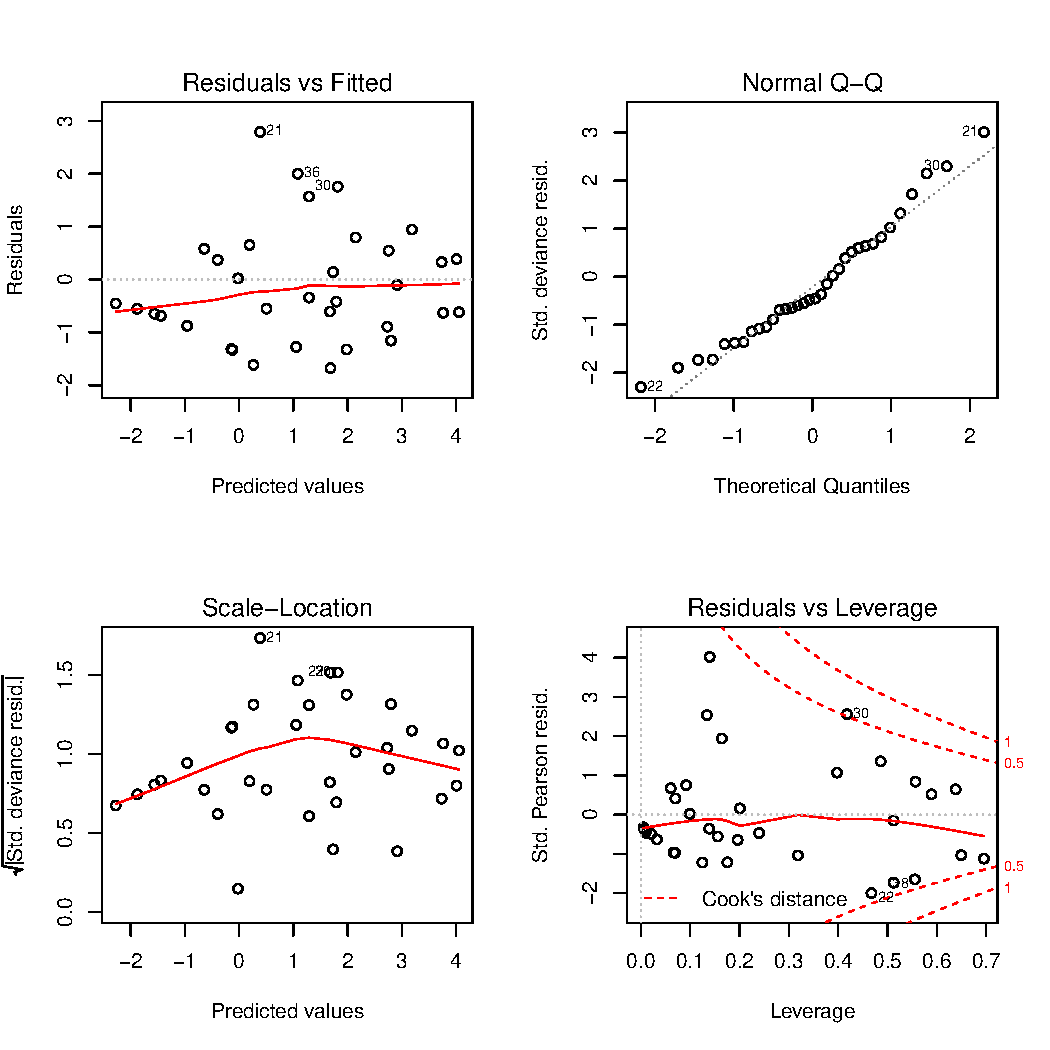
\includegraphics[width = 5cm]{figures/shipdiag.pdf}  
\end{center}
\end{frame}

\begin{frame}
\frametitle{Randomized residuals}
\begin{center}
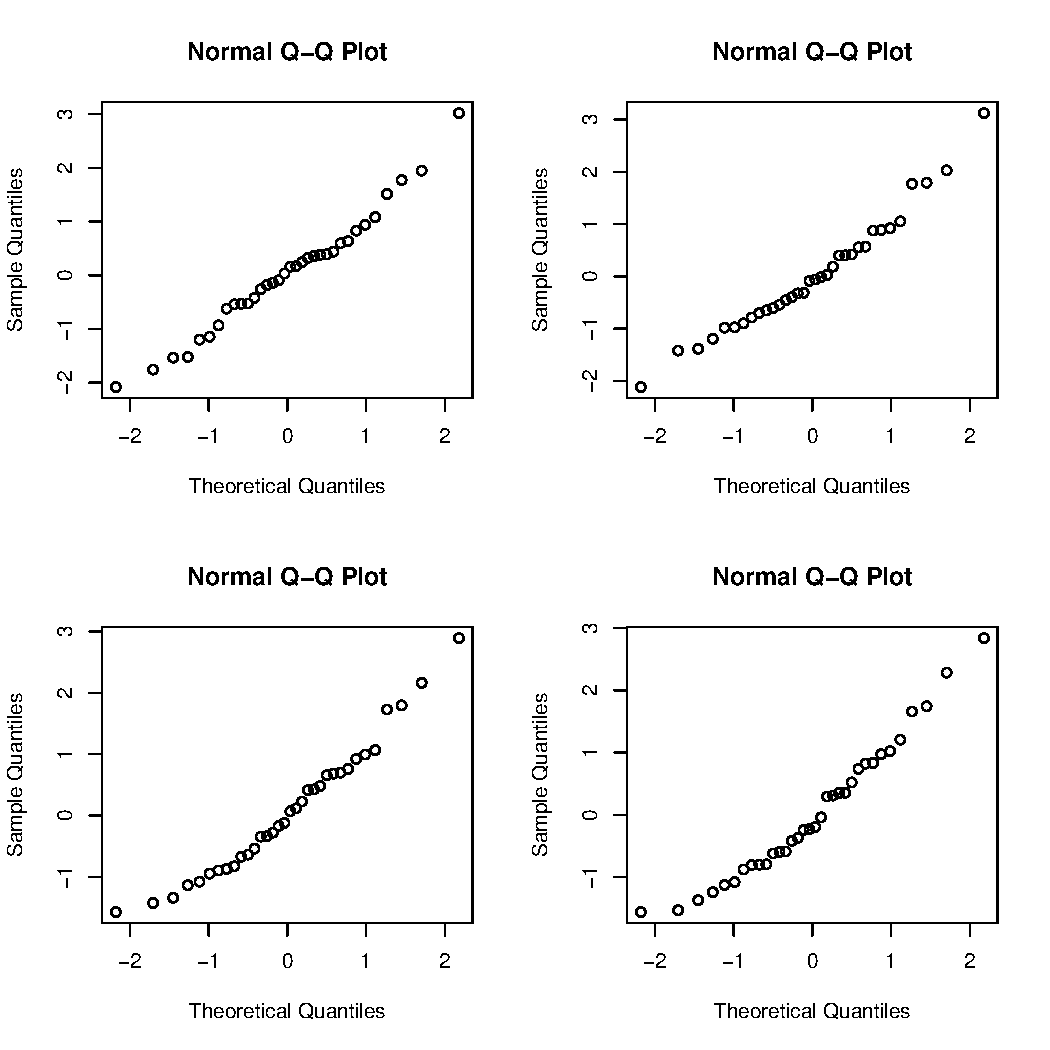
\includegraphics[width = 5.5cm]{figures/shipQQrandom.pdf}  
\end{center}

{\color{blue}Reasons for lack of fit?}

\end{frame}


\begin{frame}
\frametitle{}
If $Var(Y_i) > E(Y_i)$ the Poisson model does not hold anymore and this
phenomenon is called {\color{blue}overdispersion}. (If $Var(Y_i) < E(Y_i)$ we
have {\color{blue}underdispersion} but this latter is less common).

\bs
One of the main reasons for overdispersion is the clustering in the population
(the parameter vary from cluster to cluster, as a function of cluster size for
example). Statistically speaking, the parameter is regarded as random rather
than fixed.

\bs
A large value of the deviance may indicate overdispersion.

\bs
A first check on the data is to assume that $Var(Y_i) = \sigma^2
v_i = \sigma^2 \mu_i$ and look at the fitted value for $\sigma^2$. This is an
\textit{ad-hoc} adjustment and doesn't necessarily correspond to a
likelihood.
\end{frame}

\begin{frame}
\frametitle{}
The model cannot be fitted anymore by maximum likelihood, but via a
set of different estimating equations:
$$\sum_{i=1}^n \Big(\frac{y_i-\mu_i}{\sigma^2 v(\mu_i)}\Big) \ \frac{\partial
  \mu_i}{\partial \beta}=0,$$
that correspond to so called quasi-likelihood functions
$$\sum_{i=1}^n \int_{y_i}^{\mu_i} \frac{y_i-t}{\sigma^2 v(t)} dt.$$
\label{QL.page}
\end{frame}

\begin{frame}
\frametitle{}
\textbf{Remarks}:
\begin{itemize}
\item The maximum likelihood and the quasi-likelihood approaches give the same
estimators for all the models of the one-para\-meter exponential family (binomial,
Poisson, for example).
\item Note that $\sigma^2$ does not impact the score equations, but
  have a multiplicative impact on the standard error of the coefficients (and on
  the 
  distribution of the difference of deviances).
\end{itemize}

\bs
{see \color{red} $\bigstar$ \citeN{Gani:Scha:1992}, \citeN{Lamb:Roed:1995} and \citeN{Dean:Lawl:1989}}
\end{frame}

\begin{frame}[fragile]
\frametitle{}
\label{shipmodel.page}

{\scriptsize
\begin{lstlisting}
> ship.glm.quasi <- glm(Incidents~Ship+Year+Period+offset(log(Aggregate)),
family=quasipoisson,data=ship)
> summary(ship.glm.quasi)

Coefficients:
              Estimate Std. Error t value Pr(>|t|)    
(Intercept)   -6.40590    0.28276 -22.655  < 2e-16 ***
ShipB         -0.54334    0.23094  -2.353  0.02681 *  
ShipC         -0.68740    0.42789  -1.607  0.12072    
ShipD         -0.07596    0.37787  -0.201  0.84230    
ShipE          0.32558    0.30674   1.061  0.29864    
Year1965-69    0.69714    0.19459   3.583  0.00143 ** 
Year1970-74    0.81843    0.22077   3.707  0.00105 ** 
Year1975-79    0.45343    0.30321   1.495  0.14733    
Period1975-79  0.38447    0.15380   2.500  0.01935 *  
---
Signif. codes:  0 ‘***’ 0.001 ‘**’ 0.01 ‘*’ 0.05 ‘.’ 0.1 ‘ ’ 1

(Dispersion parameter for quasipoisson family taken to be 1.691028)

    Null deviance: 146.328  on 33  degrees of freedom
Residual deviance:  38.695  on 25  degrees of freedom
AIC: NA

Number of Fisher Scoring iterations: 5
\end{lstlisting}
}
\end{frame}

\begin{frame}
\frametitle{Parameters interpretation}

Recall the model:
\begin{eqnarray*}
\lefteqn{\log(E(\texttt{Incidents})) = \hspace*{4cm}}\\
& = & \beta_0 + \log(\texttt{Aggregate}) + \beta_1 \texttt{ship} + \beta_2
\texttt{year}  + \beta_3 \texttt{period}.
\end{eqnarray*}

\bs
In fact, each factor correspond to several parameters (number of
levels -1). For example, if we consider that ships of type A are the
reference, $\beta_1 \texttt{ship}$ is:
$$ \beta_{1B} \iota(\texttt{shipB}) +\beta_{1C} \iota(\texttt{shipC})
+ \beta_{1D} \iota(\texttt{shipD}) + \beta_{1E} \iota(\texttt{shipE}),$$
where $\iota(\texttt{ship}i)$ is a dummy variable taking the value
1 for ships of type $i$ and 0 otherwise.
\end{frame}

\begin{frame}
\frametitle{}
Therefore, $\beta_{1B}$ is the effect on $\log(\lambda)$ for ships of
type B with respect to ships of type A. The estimated value of
$\log(\lambda)$ for type B ships is -0.54334 less than that for ships
of type A (reference).  Equivalently, one can say that the
estimated expected number of damages $\lambda$ is multiplied by
$\exp(-0.54334)=0.58$ for type B ships with respect to type A ships,
and therefore reduced.

\bs
Ships of type B and C have the lowest risk, Ship of type E the
highest.

\bs
The oldest ships seems to be the safest, with those built between
1970-74 having the highest risk.
\end{frame}

\begin{frame}
\frametitle{}
\textbf{Remark on factor covariates}:

In the dummy approach used
above, a reference has to be defined (sometimes in a very arbitrary
way). The effect of this reference level is melt into the
intercept. Interpretation is with respect to the reference. (Here the
constraint is $\beta_{1A}=0$).

The default in R is to take the first category (alphabetical order) as the
reference. This can be changed by redefining the factor with the function
\texttt{relevel}.

\bs
Alternatively, one could use a different set of
{\color{blue}contrasts}, for example those where the effect of each
variable is contrasted against an overall mean. The interpretation of
the coefficients in this case is different. (Here the constraint is
$\sum_{i=1}^5 \beta_{1i}=0$).
\end{frame}

\begin{frame}
\frametitle{Alternative approach to address overdispersion }

Use a different model,
for example the {\color{blue}negative binomial} distribution (for
$y=0,1,2,\dots$):
$$P(Y_i=y_i) = \frac {\Gamma(y_i+\vartheta)}{\Gamma(\vartheta)\Gamma(y_i+1)}\left(\frac{\vartheta}{\mu_i+\vartheta}\right)^\vartheta
\left(\frac{\mu_i}{\mu_i+\vartheta}\right)^{y_i},$$ 
where $\Gamma(t)= \int_0^{\infty} e^{-x} x^{t-1}dx$ (for integer $x$,
$\Gamma(x) = (x-1)!$).

Under this model $E(Y_i)= \mu_i$ and $Var(Y_i)= \mu_i(\mu_i+1/\vartheta)$.
\end{frame}

\begin{frame}
\frametitle{}

Overdispersion can also occur with  binomial data. Either use a
``quasi-type'' model with $Var(Y_i) = \sigma^2 v(\mu_i)$ or the
{\color{blue}beta-binomial} distribution ($y=0, 1, \ldots, m_i$):
$$P(Y_i=y_i) = \left(
\begin{array}{cc}
m_i\\
y_i
\end{array} \right) \frac{B(\alpha+y_i,m_i+\beta-y_i)}{B(\alpha,\beta)},$$
where $B(u,v) = \int_0^1 x^{u-1}(1-x)^{v-1}dx$.

\bs
Here $E(Y_i) = m_i p_i$ and $Var(Y_i) = m_i p_i (1-p_i) (1 + (m_i-1) \tau^2)$,
where $p_i$ and $\tau$ depends on $\alpha$ and $\beta$.

\bs
The functions \texttt{glm.nb} (package \texttt{MASS}) and
\texttt{negbin,betabin} (package \texttt{aod}) allows to fit these models.

\end{frame}

\subsection{What can go wrong.....No overlap / (Quasi)-separation}
\begin{frame}
\frametitle{(Quasi)-separation in binary regression}

If the 0 and 1 responses can be (nearly) separated on the basis of their
covariates values ({\color{blue}no overlap, or separation }), then there is no solution to the
score equations for the binary regression (or the solution is
$\beta=\infty$).

\bs
\textbf{Example}: Analysis of recreational trips to evaluate the sensitivity of
resource usage to entrance charges and costs (\citeNP{Gurm:Triv:1996}).
\end{frame}

\begin{frame}
Available variables:
\begin{itemize}
\item TRIPS: Number of boating trips to Lake Somerville, East Texas, in 1980
\item SO: Facility's subjective quality ranking
\item SKI: Respondent's taste for water-skiing 
\item I: Income - categorical variable 
\item FC3: Cost dummy variable; 1 if an annual user fee is paid at Lake Somerville 
\item C1: Travel cost to Lake Conroe 
\item C3: Travel cost to Lake Somerville
\item C4: Travel cost to Lake Houston 
\end{itemize}
\end{frame}

\begin{frame}[fragile]
\frametitle{}
{\scriptsize
\begin{lstlisting}
> summary(glm((TRIPS>0)~SO+SKI+FC3+I+C1+C3+C4,family=binomial,
data=recreat))

Coefficients:
              Estimate Std. Error z value Pr(>|z|)    
(Intercept)  -2.881479   0.435663  -6.614 3.74e-11 ***
SO            1.437079   0.105799  13.583  < 2e-16 ***
SKI           0.405517   0.329754   1.230  0.21879    
FC3          15.660215 907.987771   0.017  0.98624    
I             0.026479   0.084000   0.315  0.75259    
C1            0.008255   0.027099   0.305  0.76064    
C3           -0.080926   0.017134  -4.723 2.32e-06 ***
C4            0.071124   0.021697   3.278  0.00105 ** 
---
Signif. codes:  0 ‘***’ 0.001 ‘**’ 0.01 ‘*’ 0.05 ‘.’ 0.1 ‘ ’ 1

(Dispersion parameter for binomial family taken to be 1)

    Null deviance: 866.53  on 658  degrees of freedom
Residual deviance: 299.49  on 651  degrees of freedom
AIC: 315.49

Number of Fisher Scoring iterations: 16
\end{lstlisting}
}
\end{frame}

\begin{frame}[fragile]
\frametitle{Why so?}
{\scriptsize
\begin{lstlisting}
> with(recreat, table(TRIPS > 0, FC3))
       FC3
          0   1
  FALSE 417   0
  TRUE  229  13
\end{lstlisting}
}
\begin{center}
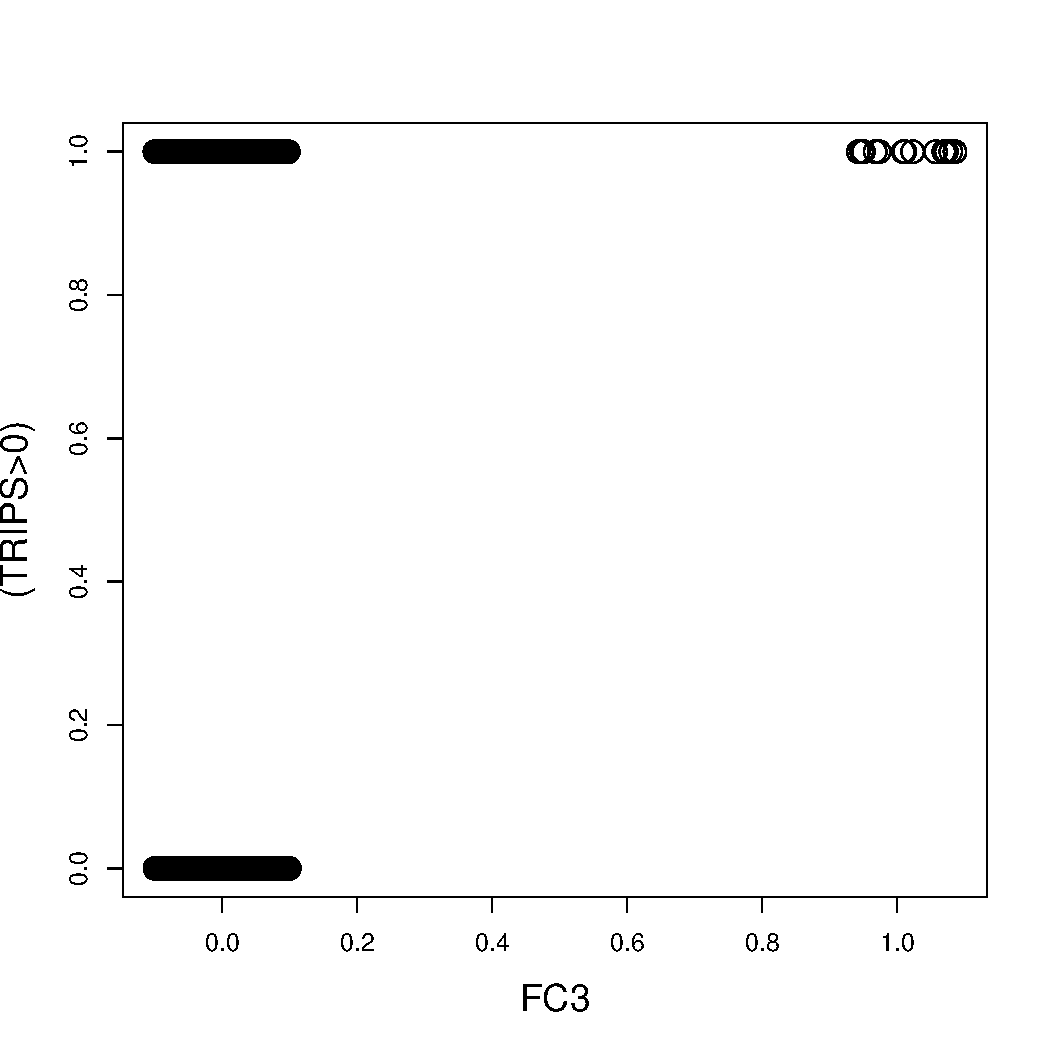
\includegraphics[width = 5.5cm]{figures/recreat.pdf}  
\end{center}

\end{frame}


\begin{frame}
\frametitle{Possible fixes:}
\begin{itemize}
\item exact logistic regression \cite{Meht:Pate:1995}.
\item robust regression approach \cite{Rous:Chri:2002}.
\item Bias reduction method \cite{Firt:1993,Kosm:Firt:2009} to
reduce finite sample bias in the GLM family. Unaffected by lack of overlap.

\bs

A corrected score function is defined $U^*(\beta) = U(\beta) -\mathcal{J}(\beta) \frac{b_1(\beta)}{n}  $
where $\mathcal{J}(\beta)$ is the Fisher information and $b_1(\beta)/n$ is
the first term in the asymptotic bias expression of the ML
estimator. It corresponds to a penalized log-likeli\-hood (canonical
specification)
$$l^*(\beta;y) = l(\beta;y) + \frac{1}{2} \log(|\mathcal{J}(\beta)|).$$

The use of AIC for model selection  is
controversial. 
\end{itemize}
\end{frame}

\begin{frame}[fragile]
\frametitle{}
{\scriptsize
\begin{lstlisting}
> summary(brglm((TRIPS>0)~SO+SKI+FC3+I+C1+C3+C4,family=binomial,
data=recreat))

Coefficients:
            Estimate Std. Error z value Pr(>|z|)    
(Intercept) -2.76325    0.41610  -6.641 3.12e-11 ***
SO           1.39492    0.10187  13.693  < 2e-16 ***
SKI          0.40403    0.32265   1.252  0.21048    
FC3          1.79847    1.71410   1.049  0.29408    
I            0.02348    0.08187   0.287  0.77424    
C1           0.01878    0.02180   0.861  0.38910    
C3          -0.08293    0.01594  -5.202 1.97e-07 ***
C4           0.06244    0.01877   3.326  0.00088 ***
---
Signif. codes:  0 ‘***’ 0.001 ‘**’ 0.01 ‘*’ 0.05 ‘.’ 0.1 ‘ ’ 1

(Dispersion parameter for binomial family taken to be 1)

    Null deviance: 836.18  on 658  degrees of freedom
Residual deviance: 300.67  on 651  degrees of freedom
Penalized deviance: 258.0502 
AIC:  316.67
\end{lstlisting}
}
\end{frame}

\subsection{What can go wrong.....Hauck-Donner phenomenon }
\begin{frame}
\frametitle{Hauck-Donner phenomenon for logistic regression}

The \texttt{z/t-value} is a Wald
approximation of the loglikelihood to test $H_0: \beta_i=0$ and is
sometimes misleading with
binomial GLM. In fact, a small value for the \texttt{z/t-value} can
either correspond to a small likelihood ratio statistic or to a
situation where $|\hat{\beta}_i|$ is large, the Wald approximation
is poor and the likelihood ratio statistic is large.
These problems can occur in cases when the fitted probabilities are
extremely close to 0 or 1.

\bs
\bs
{\color{red} $\bigstar$ \citeN{Hauc:Donn:1977}}


\end{frame}


\section{Modeling excess of zeros in count data}

\begin{frame}
\frametitle{Excess of zeros in count data}
In many applications with count data, the response contains more zeros than expected based on the Poisson (or negative binomial) distribution. We say that there is ``excess of zeros''.

\bs 
\bs 

Typical examples are: number of visits to the doctor in a given period, number
of observed animals (sharks, cods, birds) in a given habitat, number of
insurance claims in a year, etc.
\end{frame}

\begin{frame}
\frametitle{Example}

The data are a sample of German male individuals in 1994 and are taken from
\citeN{Riph:Wamb:Mill:2003}. They have been used to study the demand for health
care. 

\bs
There are  1812 observations. The outcome is \texttt{docvisits}, the number of
doctor visits in the last three months.
\end{frame}

\begin{frame}
\frametitle{}
Available covariates are: 
\begin{itemize}
\item \texttt{age} age
\item \texttt{agesq} age squared / 1000
\item \texttt{health} health satisfaction, 0 (low) - 10 (high)
\item \texttt{handicap} 1 if handicapped, 0 otherwise
\item \texttt{hdegree} degree of handicap in percentage points
\item \texttt{married} 1 if married, 0 otherwise
\item \texttt{schooling} years of schooling
\item \texttt{hhincome} household monthly income (Ger. marks / 1000)
\item \texttt{children} 1 if children under 16, 0 otherwise
\item \texttt{self} 1 if self employed, 0 otherwise
\item \texttt{civil} 1 if civil servant, 0 otherwise
\item \texttt{bluec} 1 if blue collar employee, 0 otherwise
\item \texttt{employed} 1 if employed, 0 otherwise
\item \texttt{public} 1 if public health insurance, 0 otherwise
\item \texttt{addon} 1 if add-on insurance, 0 otherwise
\end{itemize}
\end{frame}

\begin{frame}[fragile]
\frametitle{}

\begin{center}
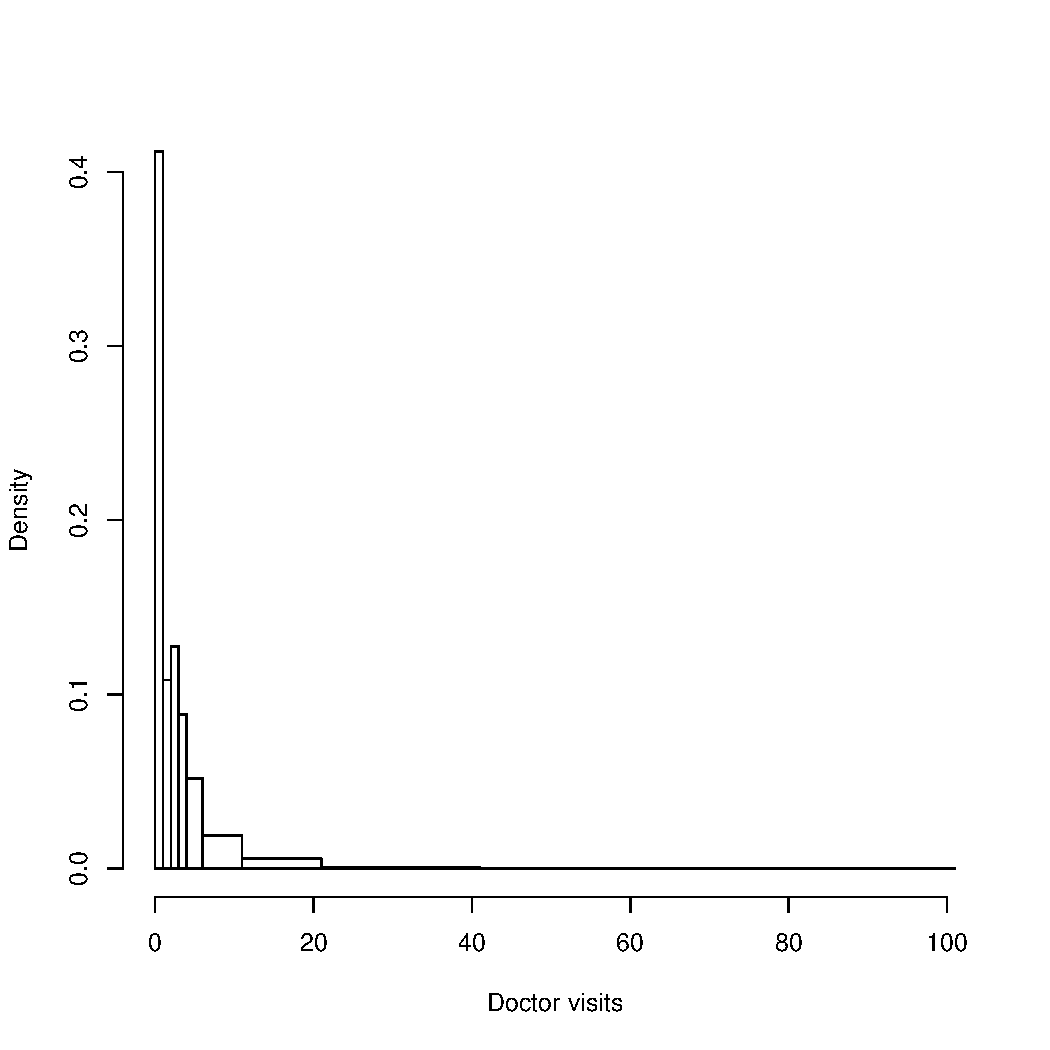
\includegraphics[width = 5cm]{figures/docvis.pdf} 
\end{center}

Proportion of zeros: $746/1812 = 41.2\%$.

{\scriptsize
\begin{lstlisting}
> mean(docvisits$docvisits)
[1] 2.958057
> mean(docvisits$docvisits[docvisits$docvisits>0])
[1] 5.028143
\end{lstlisting}
}
\end{frame}

\subsection{Models definition}
\begin{frame}
\frametitle{Hurdle (conditional, two-part, zero-altered) model}

\citeN{Mull:1986}, \citeN{Wels:Cunn:Donn:Lind:1996}

\begin{eqnarray*}
P(Y=y) & = & \left\{ \begin{array}{ll}
y=0 & \mbox{with prob. } 1-p(x)\\
y \sim \mbox{trunc.} {\mathcal P}(\lambda) & \mbox{with prob. } p(x)
\end{array} \right.\\
& & \\
& = &  \left\{
\begin{array}{ll}
(1-p(x))  & y=0\\
p(x) \frac{\exp(-\lambda(z)) \lambda(z)^y}{y! (1-\exp(-\lambda(z)))} & y=1,2,\ldots
\end{array} \right.
\end{eqnarray*}
where $x$ and $z$ are two sets of covariates that may or may not be
the same.
\end{frame}

\begin{frame}
\frametitle{}
One can for example use a logistic model for $p(x)$
$$ \log \Big(\frac{p(x)}{1-p(x)} \Big) = x^T
\beta,$$

and a log-linear type of model for $\lambda(z)$
$$\log(\lambda(z)) = z^T \gamma.$$

\bs
\textbf{Note}: A truncated negative binomial distribution can be used instead of
the truncated Poisson. 

\end{frame}

\begin{frame}
\frametitle{Zero-inflated Poisson (ZIP) model}


\citeN{Lamb:1992}

\begin{eqnarray*}
P(Y=y)  & = & \left\{ \begin{array}{ll}
y=0 & \mbox{with prob. } \pi(x)\\
y \sim {\mathcal P}(\lambda) & \mbox{with prob. } 1-\pi(x)
\end{array} \right. \\
& & \\
& = &  \left\{
\begin{array}{ll}
\pi(x) + (1-\pi(x)) \exp(-\lambda(z)) & y=0\\
(1-\pi(x)) \frac{\exp(-\lambda(z)) \lambda(z)^{y}}{y!} & y=1,2,\ldots
\end{array} \right.
\end{eqnarray*}
where $x$ and $z$ are two sets of covariates that may or may not be
the same.
\end{frame}

\begin{frame}
\frametitle{}
One can for example use a logistic model for $1-\pi(x)$
$$\log \Big(\frac{\pi(x)}{1-\pi(x)} \Big) = x^T
\alpha,$$

and a log-linear type of model for $\lambda(z)$
$$\log(\lambda(z)) = z^T \delta.$$

\bs
A negative binomial distribution can be used instead $\rightarrow$ ZINB.

\end{frame}

\begin{frame}
\frametitle{}
\textbf{Note}: 

\begin{itemize}
\item $p(x)$ in the hurdle model is the probability of ``crossing the hurdle''
(i.e.\ $y_i>0$).
\item $\pi(x)$ in the ZIP model is the probability of observing a zero from the
spike at zero.
\end{itemize}
\end{frame}

\begin{frame}
\frametitle{}
\begin{center}
\begin{tabular}{cc}
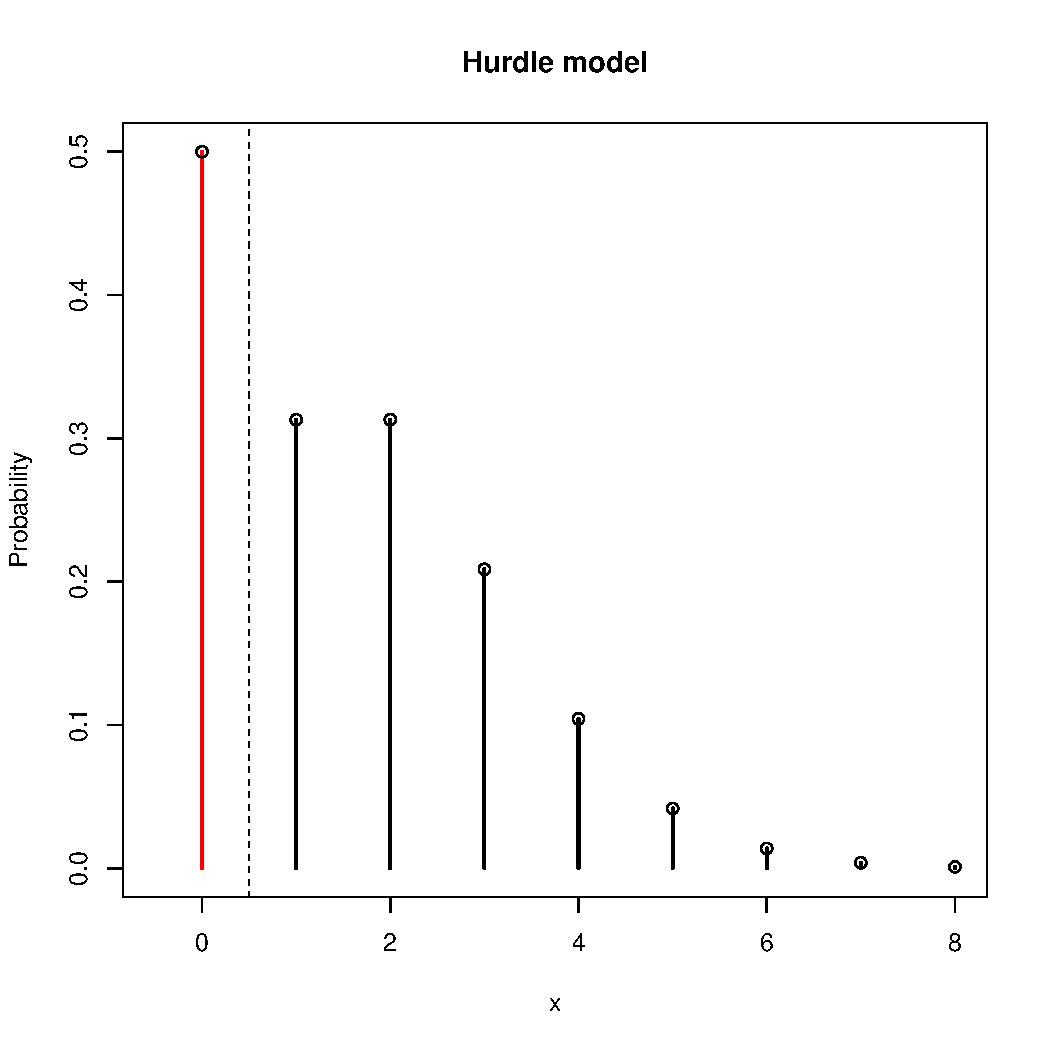
\includegraphics[width = 5cm]{figures/Hurdlemodel.pdf}  & 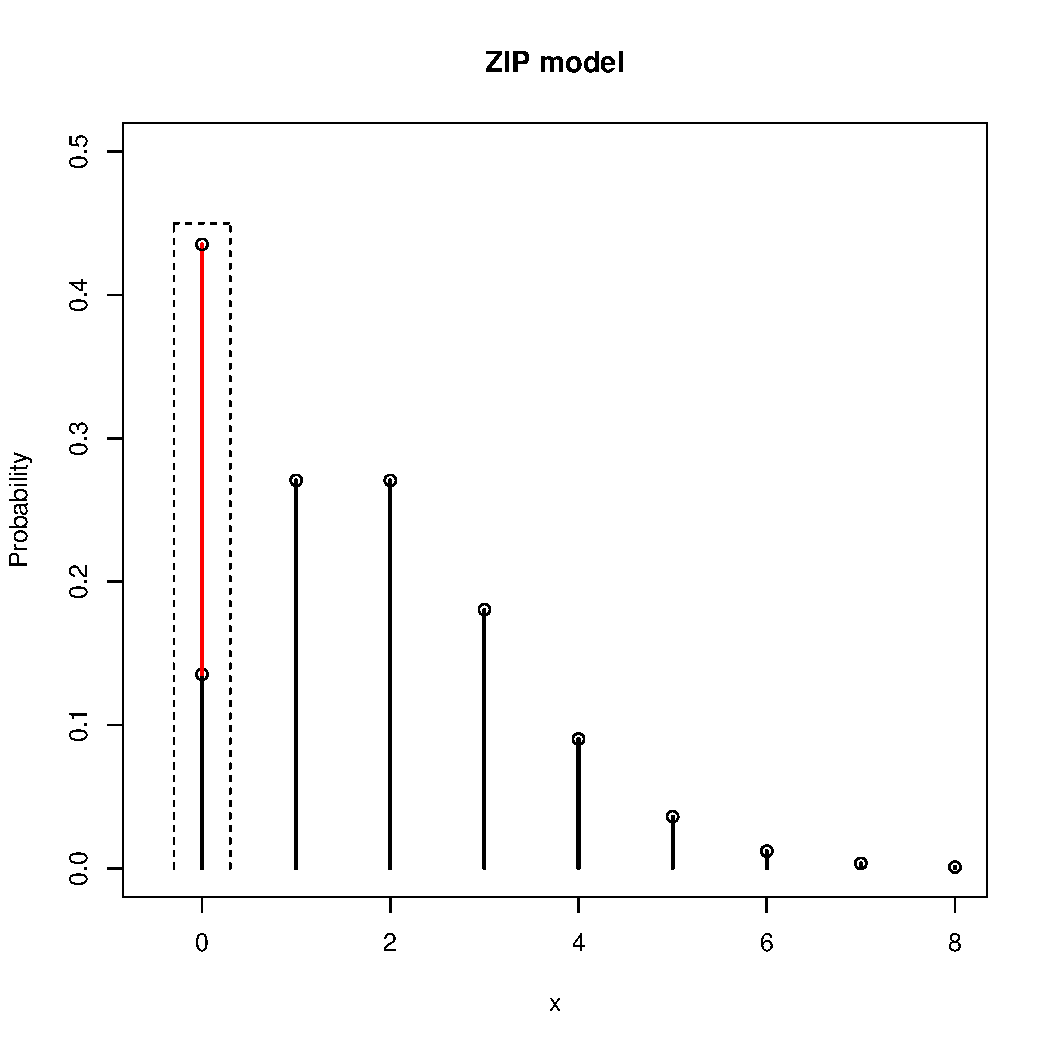
\includegraphics[width =5cm]{figures/ZIPmodel.pdf} 
\end{tabular}
\end{center}
\end{frame}

\begin{frame}
\frametitle{Moments}


Recall that $\lambda_i$ is the expectation (and the variance) of a Poisson
distribution. 

\bs
\bs
\textbf{Hurdle model}

The expectation of a truncated Poisson variable is
$\frac{\lambda_i}{1-\exp(-\lambda_i)}$, and therefore:
$$E(Y_i) = p(x_i) \frac{\lambda_i}{1-\exp(-\lambda_i)} =  p(x_i) E(Y_i|Y_i>0)$$
$$Var(Y_i) = p(x_i) \frac{\lambda_i + \lambda_i^2}{1-\exp(-\lambda_i)} -
\Big(p(x_i)\frac{\lambda_i}{1-\exp(-\lambda_i)}\Big)^2$$ 
\bs

In this model $Var(Y_i)$ can be either larger or smaller than $E(Y_i)$
accounting for overdispersion or underdispersion.
\end{frame}

\begin{frame}
\frametitle{}
\textbf{ZIP model}
$$E(Y_i) = (1-\pi(x_i)) \lambda_i$$
$$Var(Y_i) = (1-\pi(x_i)) (\lambda_i+\pi(x_i) \lambda_i^2)$$

\bs
For this model $Var(Y_i) > E(Y_i)$ (overdispersion) if $\pi(x_i)>0$.

\bs
\bs
In both models, the quantity are estimated by plugging-in the estimates of the
parameters. 

\end{frame}

\begin{frame}
\frametitle{Estimation - Hurdle models}

With a logistic model for $p(x)$
$$\mbox{logit}(p(x)) = \log \Big(\frac{p(x)}{1-p(x)} \Big) = x^T
\beta,$$

and a log-linear model for $\lambda(z)$
$$\log(\lambda(z)) = z^T \gamma,$$

the likelihood $L(\beta,\gamma)$ for the hurdle Poisson model is
\begin{eqnarray*}
\lefteqn{L(\beta,\gamma) = \prod_{i=1}^n P(Y_i = y_i) = }\\
&&\prod_{i=1}^n (1-p(x_i))^{\iota(y_i=0)}  \left( p(x_i)\frac{\exp(-\lambda(z_i))
\lambda(z_i)^{y_i}}{y_i! (1-\exp(-\lambda(z_i)))} \right)^{\iota(y_i>0)},
\end{eqnarray*}
where $\iota(A)=1$ if $A$ is true and $0$ otherwise.
\end{frame}

\begin{frame}
\frametitle{}
The log-likelihood $l(\beta,\gamma)$ is:
\begin{eqnarray*}
\lefteqn{l(\beta,\gamma) =  \sum_{i=1}^n \iota(y_i=0) \log(1-p(x_i)) + }\\
& & \sum_{i=1}^n \iota(y_i>0) \left[ \log(p(x_i)) -\lambda(z_i) + y_i
\log(\lambda(z_i)) \right.\\
& &\left. - \log(y_i!) - \log(1-\exp(-\lambda(z_i))) \right]  \\
& = & \sum_{y_i=0} \log\Big( \frac{1}{1+\exp(x_i^T \beta)} \Big) + \sum_{y_i>0} \log\Big(\frac{\exp(x_i^T \beta)}{1+\exp(x_i^T \beta)} \Big)+\\
& & \sum_{y_i>0} \Big(y_i z_i^T \gamma - \exp(z_i^T \gamma) -  \log(1- \exp(-\exp(z_i^T \gamma))) - \log(y_i!)\Big)\\
& = & l(\beta)+l(\gamma)
\end{eqnarray*}

\end{frame}

\begin{frame}
\frametitle{}
The components in $l(\beta,\gamma)$ can be fitted separately (orthogonal parameters).

\bs
\bs
\textbf{Note}: The logistic link can be replaced by other links for the binomial
family, and the expressions updated accordingly. 

\bs
\textbf{Note}: The log-likelihood for the conditional negative binomial model
is obtained similarly. 

\end{frame}

\begin{frame}[allowframebreaks]
\frametitle{}
The two independent parts of a Poisson hurdle models can also be fitted by exploiting the GLM
framework \cite{Barr:Wels:2002}:

\begin{enumerate}
\item A binary (logistic) regression to separate the zero from the positive
(using all the data, and coding 1 all the positive values). 

\item A truncated Poisson GLM for the positive (using only the portion of data
corresponding to the positive responses).

\bs 
The expectation of a truncated Poisson variable is
$$\mu = h(\lambda) = \frac{\lambda}{1-\exp(-\lambda)},$$
so $\lambda=h^{-1}(\mu)$.

\bs With $\log(\lambda) = z^T \gamma $, it gives $\log(h^{-1}(\mu)) = z^T \gamma,$ 
so the link function is $g(x) = \log(h^{-1}(x))$.

Also, the variance of a truncated Poisson variable is
$$v(\mu) = \mu (1 + h^{-1}(\mu) -\mu),$$
and the deviance
\begin{eqnarray*}
\lefteqn{D(y;\mu) = 2 \Big[ y \log(h^{-1}(\mu)) - h^{-1}(\mu)} \\
 & & \log(1-\exp(h^{-1}(\mu))) - y \log(h^{-1}(y)) \\
 & & h^{-1}(y) + \log(1-\exp(h^{-1}(y))) \Big]
\end{eqnarray*}

\label{truncpoisdef}
Use the GLM setting with the above specifications.

 \bs \textbf{Remark}: Cannot invert $h$ explicitly.
\end{enumerate}

\end{frame}

\begin{frame}
\frametitle{Estimation - ZIP models}

With a logistic model for $\pi(x)$
$$\log \Big(\frac{ \pi(x)}{1-\pi(x)} \Big) = x^T
\alpha,$$

and a log-linear model for $\lambda(z)$
$$\log(\lambda(z)) = z^T \delta,$$

\bs the likelihood $L(\alpha,\delta)$ for the ZIP model is
\end{frame}

\begin{frame}
\frametitle{}
\begin{eqnarray*}
\lefteqn{L(\alpha,\delta) = \prod_{i=1}^n P(Y_i = y_i) = }\\
&&\prod_{i=1}^n (\pi(x_i) +(1-\pi(x_i))\exp(-\lambda(z_i)))^{\iota(y_i=0)}
 \\
&& \times \left( (1-\pi(x_i))\frac{\exp(-\lambda(z_i))
\lambda(z_i)^y_i}{y_i!} \right)^{\iota(y_i>0)}
\end{eqnarray*}

\bs
This likelihood has to be maximized jointly for $(\alpha,\delta)$.

\end{frame}


\begin{frame}
\frametitle{}
The ZIP model can also be fitted using the EM algorithm
\cite{Demp:Lair:Rubi:1977}. 


\bs
Let $W_i=1$ when $y_i$ is from the spike at zero, and $0$ otherwise ($W_i$ is
unknown). The likelihood becomes
\begin{eqnarray*}
\lefteqn{L(\alpha,\delta|W_i) = \prod_{i=1}^n P(Y_i = y_i) = }\\
&&\prod_{i=1}^n \pi(x_i)^{W_i \iota(y_i=0)} \times (1-\pi(x_i))^{1-W_i}
  \times \left( \frac{\exp(-\lambda(z_i))
\lambda(z_i)^y_i}{y_i!} \right)^{1-W_i}
\end{eqnarray*}

\bs
Conditioning on $W_i$ and using the EM algorithm, has the effect to separate the
components. 
\end{frame}

\begin{frame}
\frametitle{Sources of zeros}

Sometimes one likes to discriminate between various type of zeros. There are at
least 4 sorts of zeros, see \citeN{Zuur:Ieno:Walk:Save:Smit:2009}: 


\begin{enumerate}
\item structural zeros (e.g.\ animal not present, because habitat not suitable).
\item design error, poor experimental design or sampling practices are the reason (e.g.\ sampling at the wrong time, for too short a time period, in too small an area).  
\item observer error (e.g.\ species that are difficult to identify).
\item ``bird'' error: the habitat is suitable, but the site is not used.
\end{enumerate}
\end{frame}

\subsection{Comparison of ZIP and hurdle models} 
\begin{frame}
\frametitle{}

\begin{center}
\begin{tabular}{cc}
Hurdle model & ZIP model\\
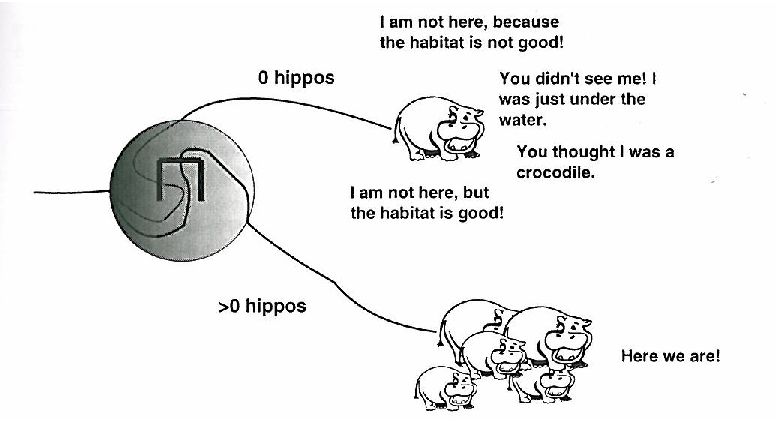
\includegraphics[width = 5.5cm]{figures/114fromtiff.pdf}  & 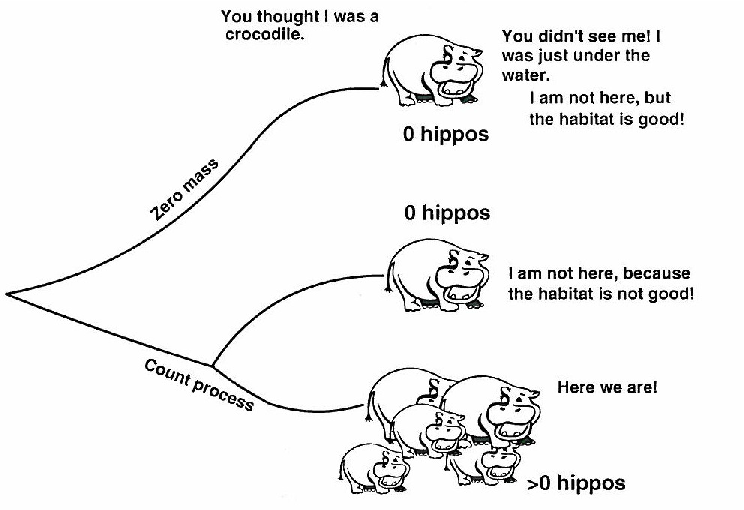
\includegraphics[width =5.5cm]{figures/115fromtiff.pdf} 
\end{tabular}
\end{center}

\bs
Figures from \shortciteN{Zuur:Ieno:Walk:Save:Smit:2009}.

\end{frame}


\begin{frame}
\frametitle{}
\begin{tabular}{l|l|l}
Model & Hurdle & ZIP\\
\hline
&&\\
Parametrisation & orthogonal & not orthogonal \\
&&\\
Estim.\ equations & separate & involve all parameters \\
&&\\
Fit components & separately & simultaneously \\ 
&& or use EM to separate\\
&&\\
Interpret param.\ & separately & simultaneously\\
&&\\
& $p_i()=$ & $\pi()$\\
& presence prob.\ & mixing prob.\ \\
&&\\
& cond. abundance & null abundance 
\end{tabular}
\end{frame}


\begin{frame}[fragile]
\frametitle{Hurdle fit of doctor visits data: abundance.}

{\scriptsize
\begin{lstlisting}
Count model coefficients (truncated poisson with log link):
             Estimate Std. Error z value Pr(>|z|)    
(Intercept)  2.711909   0.274745   9.871  < 2e-16 ***
age         -0.019347   0.012227  -1.582 0.113573    
agesq        0.340346   0.138224   2.462 0.013805 *  
health      -0.165889   0.006030 -27.510  < 2e-16 ***
handicap     0.360922   0.073755   4.893 9.91e-07 ***
hdegree     -0.004873   0.001263  -3.859 0.000114 ***
married     -0.150048   0.039991  -3.752 0.000175 ***
schooling   -0.001591   0.007247  -0.220 0.826214    
hhincome     0.005181   0.007607   0.681 0.495784    
children     0.106423   0.038281   2.780 0.005435 ** 
self        -0.183134   0.071802  -2.551 0.010755 *  
civil       -0.123018   0.079012  -1.557 0.119481    
bluec        0.077810   0.039401   1.975 0.048285 *  
employed    -0.111501   0.046732  -2.386 0.017034 *  
public       0.109596   0.069555   1.576 0.115100    
addon        0.261478   0.094248   2.774 0.005531 ** 
\end{lstlisting}
}

\end{frame}


\begin{frame}[fragile]
\frametitle{Hurdle fit of doctor visits data: presence/absence.}

{\scriptsize
\begin{lstlisting}
Zero hurdle model coefficients (binomial with logit link):
             Estimate Std. Error z value Pr(>|z|)    
(Intercept)  4.228318   0.970927   4.355 1.33e-05 ***
age         -0.100415   0.045999  -2.183   0.0290 *  
agesq        1.252381   0.537255   2.331   0.0197 *  
health      -0.314382   0.028633 -10.980  < 2e-16 ***
handicap     0.125226   0.427901   0.293   0.7698    
hdegree      0.003857   0.008130   0.474   0.6352    
married      0.227869   0.147236   1.548   0.1217    
schooling   -0.004350   0.023410  -0.186   0.8526    
hhincome     0.032699   0.026482   1.235   0.2169    
children    -0.329635   0.134636  -2.448   0.0144 *  
self        -0.245749   0.199960  -1.229   0.2191    
civil       -0.235280   0.214703  -1.096   0.2731    
bluec        0.029496   0.135280   0.218   0.8274    
employed     0.036584   0.182606   0.200   0.8412    
public       0.051585   0.187571   0.275   0.7833    
addon       -0.034627   0.379243  -0.091   0.9272    
\end{lstlisting}
}

\end{frame}

\begin{frame}[fragile]
\frametitle{ZIP fit of doctor visits data: abundance.}

{\scriptsize
\begin{lstlisting}
Count model coefficients (poisson with log link):
             Estimate Std. Error z value Pr(>|z|)    
(Intercept)  2.696432   0.275366   9.792  < 2e-16 ***
age         -0.018650   0.012254  -1.522 0.128015    
agesq        0.332125   0.138565   2.397 0.016535 *  
health      -0.165427   0.006021 -27.473  < 2e-16 ***
handicap     0.361505   0.073723   4.904 9.41e-07 ***
hdegree     -0.004890   0.001263  -3.872 0.000108 ***
married     -0.149734   0.039960  -3.747 0.000179 ***
schooling   -0.001747   0.007231  -0.242 0.809124    
hhincome     0.005360   0.007530   0.712 0.476584    
children     0.102861   0.038276   2.687 0.007202 ** 
self        -0.180518   0.072126  -2.503 0.012321 *  
civil       -0.124073   0.079062  -1.569 0.116575    
bluec        0.077995   0.039393   1.980 0.047710 *  
employed    -0.111584   0.046757  -2.386 0.017012 *  
public       0.111776   0.069614   1.606 0.108349    
addon        0.258275   0.094552   2.732 0.006303 ** 
\end{lstlisting}
}

\end{frame}

\begin{frame}[fragile]
\frametitle{ZIP fit of doctor visits data: presence/absence.}

{\scriptsize
\begin{lstlisting}
Zero-inflation model coefficients (binomial with logit link):
             Estimate Std. Error z value Pr(>|z|)    
(Intercept) -4.248435   1.016598  -4.179 2.93e-05 ***
age          0.103531   0.048036   2.155   0.0311 *  
agesq       -1.264186   0.560348  -2.256   0.0241 *  
health       0.292041   0.029418   9.927  < 2e-16 ***
handicap    -0.065816   0.435600  -0.151   0.8799    
hdegree     -0.005067   0.008355  -0.607   0.5442    
married     -0.274227   0.154044  -1.780   0.0750 .  
schooling    0.003972   0.024582   0.162   0.8716    
hhincome    -0.032490   0.027708  -1.173   0.2410    
children     0.361796   0.141202   2.562   0.0104 *  
self         0.202949   0.213576   0.950   0.3420    
civil        0.201870   0.229784   0.879   0.3797    
bluec       -0.013367   0.140868  -0.095   0.9244    
employed    -0.057557   0.188931  -0.305   0.7606    
public      -0.012178   0.200784  -0.061   0.9516    
addon        0.077311   0.385901   0.200   0.8412  
\end{lstlisting}
}

\end{frame}

\begin{frame}
\frametitle{Model validation and inference}

Both the hurdle and the ZIP model are fitted by using the likelihood. All the
inferential methods therefore apply: likelihood ratio tests, Akaike criterion
(AIC), etc.

\bs
The Poisson hurdle model being separable, the inference on its two
components can be carried over separately. In addition, the GLM framework fully
applies and one can look at the deviance as well. 


\bs
\bs
Graphical validation tools are not implemented in the package \texttt{pscl}.
\end{frame}

\subsection{Analysis of the origin of gender differences in science}
\begin{frame}
\frametitle{Gender differences in science}
Study analyzing the established presence of gender differences in science, see
 \citeN{Long:1990}.
 
\bs
A sample of 915 biochemistry graduate students. The response is \texttt{art},
that is the count of articles produced during the last 3 years of Ph.D. 

\begin{itemize}
\item \texttt{fem} factor indicating student gender (Men or Women)
\item \texttt{mar} factor indicating student marital status (Single or Married)
\item \texttt{kid5} number of children aged 5 or younger
\item \texttt{phd} prestige of Ph.D. program, based on Cartter, Roose and
Andersen, and Jones et al studies.
\item \texttt{ment} count of articles produced by Ph.D.\ mentor during last 3
years 
\end{itemize}
\end{frame}


\begin{frame}
\frametitle{}
\begin{center}
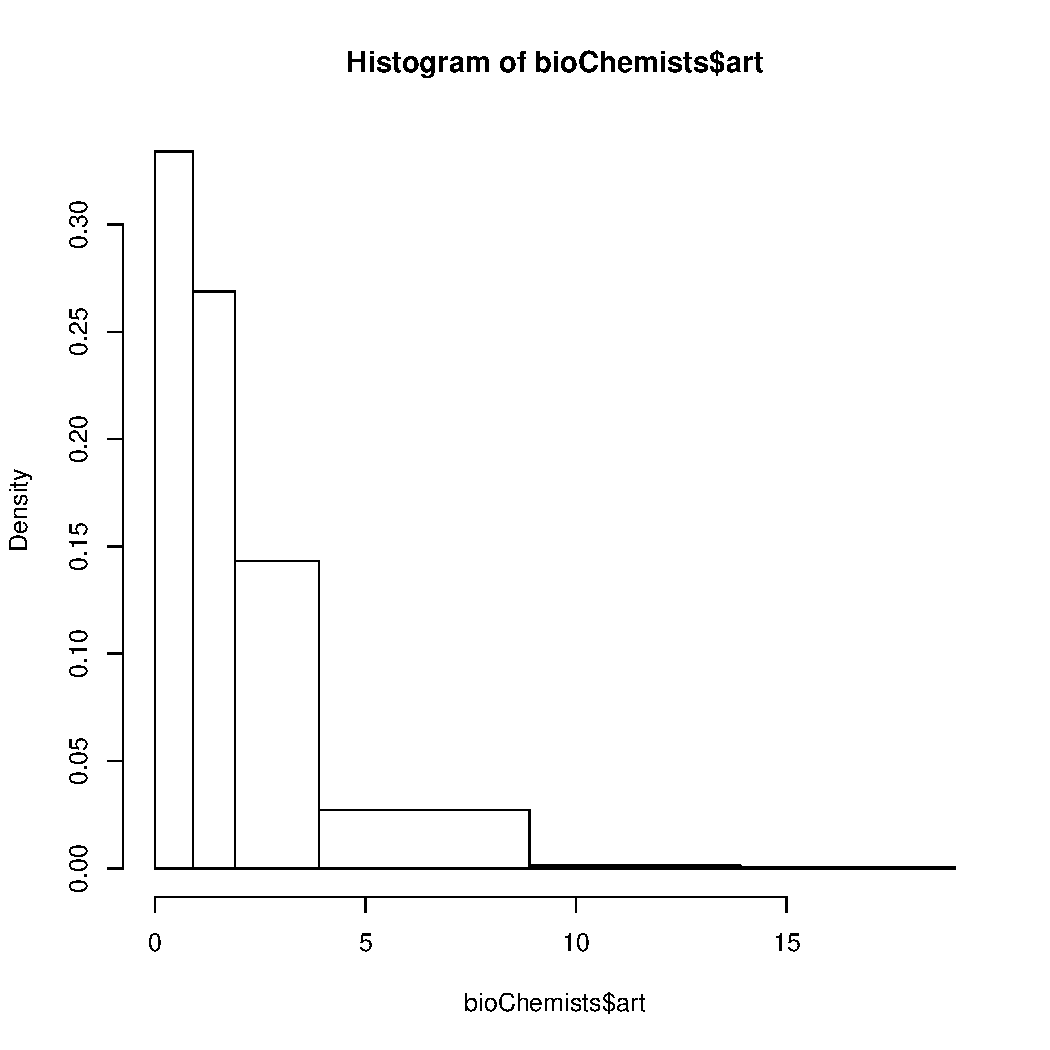
\includegraphics[width = 7cm]{figures/BioC.pdf}  
\end{center}
\end{frame}

\begin{frame}[fragile]
\frametitle{}
{\scriptsize
\begin{lstlisting}
Count model coefficients (truncated poisson with log link):
            Estimate Std. Error z value Pr(>|z|)    
(Intercept)  0.67114    0.12246   5.481 4.24e-08 ***
femWomen    -0.22858    0.06522  -3.505 0.000457 ***
marMarried   0.09649    0.07283   1.325 0.185209    
kid5        -0.14219    0.04845  -2.934 0.003341 ** 
phd         -0.01273    0.03130  -0.407 0.684343    
ment         0.01875    0.00228   8.222  < 2e-16 ***
Zero hurdle model coefficients (binomial with logit link):
            Estimate Std. Error z value Pr(>|z|)    
(Intercept)  0.23680    0.29552   0.801   0.4230    
femWomen    -0.25115    0.15911  -1.579   0.1144    
marMarried   0.32623    0.18082   1.804   0.0712 .  
kid5        -0.28525    0.11113  -2.567   0.0103 *  
phd          0.02222    0.07956   0.279   0.7800    
ment         0.08012    0.01302   6.155 7.52e-10 ***
---
Signif. codes:  0 '***' 0.001 '**' 0.01 '*' 0.05 '.' 0.1 ' ' 1 

> extractAIC(bioChurdle)
[1]   12.000 3234.623
\end{lstlisting}
}

\end{frame}

\begin{frame}[fragile]
\frametitle{}
{\scriptsize
\begin{lstlisting}
Count model coefficients (truncated poisson with log link):
              Estimate Std. Error z value Pr(>|z|)    
(Intercept)    0.65835    0.12440   5.292 1.21e-07 ***
femWomen      -0.20919    0.07283  -2.872  0.00408 ** 
kid5          -0.12937    0.05276  -2.452  0.01421 *  
marMarried     0.09998    0.07304   1.369  0.17106    
phd           -0.01209    0.03130  -0.386  0.69922    
ment           0.01879    0.00228   8.242  < 2e-16 ***
femWomen:kid5 -0.06613    0.11152  -0.593  0.55323    
Zero hurdle model coefficients (binomial with logit link):
              Estimate Std. Error z value Pr(>|z|)    
(Intercept)    0.25256    0.30450   0.829   0.4069    
femWomen      -0.27119    0.18436  -1.471   0.1413    
kid5          -0.29739    0.12455  -2.388   0.0170 *  
marMarried     0.32078    0.18258   1.757   0.0789 .  
phd            0.02140    0.07965   0.269   0.7882    
ment           0.08015    0.01302   6.155 7.52e-10 ***
femWomen:kid5  0.04861    0.22555   0.216   0.8293    
---
Signif. codes:  0 '***' 0.001 '**' 0.01 '*' 0.05 '.' 0.1 ' ' 1 

> extractAIC(bioChurdlewithint)
[1]   14.000 3238.217
\end{lstlisting}
}
\end{frame}

\begin{frame}[fragile]
\frametitle{Submodel 1}

{\scriptsize
\begin{lstlisting}
Count model coefficients (truncated poisson with log link):
            Estimate Std. Error z value Pr(>|z|)    
(Intercept)  0.67114    0.12246   5.481 4.24e-08 ***
femWomen    -0.22858    0.06522  -3.505 0.000457 ***
marMarried   0.09649    0.07283   1.325 0.185209    
kid5        -0.14219    0.04845  -2.934 0.003341 ** 
phd         -0.01273    0.03130  -0.407 0.684343    
ment         0.01875    0.00228   8.222  < 2e-16 ***
Zero hurdle model coefficients (binomial with logit link):
            Estimate Std. Error z value Pr(>|z|)    
(Intercept)  0.32116    0.11814   2.718  0.00656 ** 
kid5        -0.14306    0.09484  -1.508  0.13144    
ment         0.08086    0.01248   6.479 9.25e-11 ***
---
Signif. codes:  0 '***' 0.001 '**' 0.01 '*' 0.05 '.' 0.1 ' ' 1 

> extractAIC(bioChurdlesub1)
[1]    9.000 3235.348
\end{lstlisting}
}

\end{frame}

\begin{frame}[fragile]
\frametitle{Submodel 2}
{\scriptsize
\begin{lstlisting}
Count model coefficients (truncated poisson with log link):
             Estimate Std. Error z value Pr(>|z|)    
(Intercept)  0.691554   0.054696  12.644  < 2e-16 ***
femWomen    -0.238888   0.064766  -3.688 0.000226 ***
kid5        -0.114713   0.044280  -2.591 0.009580 ** 
ment         0.018433   0.002228   8.275  < 2e-16 ***
Zero hurdle model coefficients (binomial with logit link):
            Estimate Std. Error z value Pr(>|z|)    
(Intercept)  0.24871    0.10766   2.310   0.0209 *  
ment         0.08092    0.01249   6.477 9.39e-11 ***
---
Signif. codes:  0 '***' 0.001 '**' 0.01 '*' 0.05 '.' 0.1 ' ' 1 

Number of iterations in BFGS optimization: 9 
Log-likelihood: -1611 on 6 Df
> extractAIC(bioChurdlesub2)
[1]    6.000 3233.664
\end{lstlisting}
}
\end{frame}

\begin{frame}[fragile]
\frametitle{ZIP fit}
{\scriptsize
\begin{lstlisting}
Count model coefficients (poisson with log link):
             Estimate Std. Error z value Pr(>|z|)    
(Intercept)  0.640838   0.121307   5.283 1.27e-07 ***
femWomen    -0.209145   0.063405  -3.299 0.000972 ***
marMarried   0.103751   0.071111   1.459 0.144565    
kid5        -0.143320   0.047429  -3.022 0.002513 ** 
phd         -0.006166   0.031008  -0.199 0.842378    
ment         0.018098   0.002294   7.888 3.07e-15 ***

Zero-inflation model coefficients (binomial with logit link):
             Estimate Std. Error z value Pr(>|z|)   
(Intercept) -0.577059   0.509386  -1.133  0.25728   
femWomen     0.109746   0.280082   0.392  0.69518   
marMarried  -0.354014   0.317611  -1.115  0.26502   
kid5         0.217097   0.196482   1.105  0.26919   
phd          0.001274   0.145263   0.009  0.99300   
ment        -0.134114   0.045243  -2.964  0.00303 **
---
Signif. codes:  0 '***' 0.001 '**' 0.01 '*' 0.05 '.' 0.1 ' ' 1 
\end{lstlisting}
}
\end{frame}

\section{Generalized Estimating Equations}
\label{GEE.section}

\begin{frame}
\frametitle{Longitudinal data}
In {\color{blue}longitudinal studies} (in contrast with
cross-sectional studies) individuals are measured repeatedly over
time. Longitudinal are also called {\color{blue}panel data} (mostly in
economics).

\bs
Independence is assumed between individuals (as in GLM), but not between
measurements of the same individual.

\bs
Longitudinal studies can distinguish changes over time within
individuals.

\bs
Sometime {\color{blue}clusters} are defined by other groups than an
individual (medical practices, cities, etc.).

\bs
\textbf{Notation}: see page~\pageref{Ximatrix}.
\end{frame}

\begin{frame}
\frametitle{Possible approaches to repeated measurements}
Model $Y_{it}$ by means of $x_{it}$:
\begin{itemize}
\item {\color{blue}Marginal models} (as in cross-sectional studies):\\
not only $g(E(Y_{it})) = x_{it}^T \beta$ ($t=1,\ldots,n_i$), but also $Var(Y_i) = V_i(\phi,\alpha)$.
\item {\color{blue}Random (or mixed) effects model}: the correlation among
  repeated responses is
  implied by varying regression coefficients across individuals:\\
$g(E(Y_{it}|\gamma_i)) = x_{it}^T \beta + z_{it}^T \gamma_i$, and $\gamma_i$ are iid
from a  distribution with $E(\gamma_i)=0$ and $Var(\gamma_i)= \sigma^2_{\gamma}I$.

A large literature exists for these models in the Gaussian, identity-link case,
much less for other distributions of the exponential family (GLMM models).
\end{itemize}

\end{frame}

\subsection{Model specification}
\begin{frame}[allowframebreaks]
\frametitle{Marginal models}
The inference drawn from the marginal model is {\color{blue}population average} versus the {\color{blue}subject specific} that can be drawn from the random effect models.

\bs
Ingredients of the model:
\begin{itemize}
\item The marginal expectation of the response $E(Y_{it}) = \mu_{it}$
  depends on a set of explanatory variables $x_{it}$ via $g(\mu_{it})
  = x_{it}^T \beta$, where $g$ is the link function (same or similar choices as for GLM).
\item The marginal variance depends on the marginal mean $Var(Y_{it})
  = \phi v(\mu_{it}) $.
\item The correlation between $Y_{it}$ and $Y_{it^\prime}$ is a function of
  the marginal means and perhaps of additional parameters $\alpha$.
\end{itemize}

\bs
$\beta$ is the parameter of interest, $\phi$ and $\alpha$ are nuisance parameters.

\bs
The parameters $\beta$ are interpreted as for GLM.

\bs
A marginal distribution for $Y_{it}$ is postulated (e.g.\ Bernoulli, Poisson). Note,
however, that this does not define a joint multivariate distribution for $Y_i$
($\leadsto$ no likelihood).

\bs\bs\bs\bs\bs\bs\bs
The regression parameters $\beta$ are estimated by the
{\color{blue}generalized estimating equations (GEE)} approach. 
By analogy with the score equations of a GLM (see
p.~\pageref{EE.GLM}), we solve (for $\beta$):
$$\sum_{i=1}^n D_i^T V_i(\alpha)^{-1} (Y_i - \mu_i) =0,$$
with $D_i = d \mu_i/ d \beta$, $V_i(\alpha) = \phi  A_i^{1/2} R(\alpha)
A_i^{1/2}$, where $A_i = \mbox{diag}(v(\mu_{it}))$ and
$R(\alpha)$ is a {\color{blue}``working'' correlation} matrix (in
contrast to the true correlation matrix $Corr(Y_i)$).

\bs
The GEE can be written in the form of an iterative reweighted least squares algorithm.
\end{frame}

\begin{frame}
\frametitle{Choices for the working correlation matrix $R(\alpha)$ }
\begin{description}
\item[{\color{blue}independence}] $R(\alpha)=I$, and we have in fact a
  GLM model.
\item[{\color{blue}fixed}] $R(\alpha)$ have a predefined known form.
\item[{\color{blue}exchangeable}] all the correlations $R(\alpha)_{t,t^\prime}$
are equal to $\alpha$. 
\item[{\color{blue}autoregressive (AR)}] correlation decreases with
  time difference, e.g.\ $R(\alpha)_{t,t^\prime} = \alpha^{|t-t^\prime|}$.
\item[{\color{blue}$m$-dependence}] Observations are correlated up to
  time distance $m$.
\item[{\color{blue}unstructured/unspecified}] $R(\alpha)$ is
  completely free (beside a diagonal of 1's and the symmetry constraint).
\end{description}
\end{frame}

\begin{frame}
\frametitle{Estimators of $\phi$ and $\alpha$}

A procedure that iterates between a
modified Fisher scoring for $\beta$ and (moment) estimation of
$\alpha$ and $\phi$ is used.

\bs
If we define $r_{it} = (y_{it} -
\mu_{it})/\sqrt{v(\mu_{it})}$, we have that
$Var(r_{it}) = \phi$.  An estimator of $\phi$ can be
obtained by  ( $N=\sum_{i=1}^n n_i$)
$$\hat{\phi} = \sum_{i=1}^n \sum_{t=1}^{n_i}
\frac{\hat{r}_{it}^2}{N-(p+1)}.$$

\sms
The specific estimator of $R(\alpha)$ depends upon the choice of the
correlation structure. The general approach is to estimate $\alpha$ by
a simple function of couples of residuals $\hat{r}_{iu}, \hat{r}_{iv}$.

\sms
Some of the correlation structure require clusters of same size, that
is, $n_i = n_{same}$ for all $i$.
\end{frame}

\begin{frame}[allowframebreaks]
\frametitle{Examples}



\begin{itemize}
\item If $R(\alpha)_{t,t^\prime}=\alpha$ (exchangeable) for all $t \neq
  t^\prime$, then given $\hat{\phi}$, we have
$$\hat{\alpha} = \frac{1}{\hat{\phi}} \sum_{i=1}^n \sum_{t>t^\prime} \hat{r}_{it}
\hat{r}_{it^\prime} /(K-(p+1)),$$
where $K = \sum_{i=1}^n 1/2 \ n_i(n_i-1)$.
\item If $(R_{\alpha,i})_{tt^\prime} = \alpha^{|t-t^\prime|}$
  (autoregressive) an  option is to use
$$\hat{\alpha}_{t,t^\prime} = \sum_{i=1}^n \frac{\sum_{t=1}^{n_i-(t-t^\prime)}\hat{r}_{it}
\hat{r}_{it^\prime}}{n_i}.$$ 
\item $\alpha = (\alpha_1, \ldots, \alpha_{n_{same}-1})$, where
  $\alpha_t = R(\alpha)_{t,t+1}$. Then
$$\hat{\alpha}_t = \frac{1}{\hat{\phi}} \sum_{i=1}^n \hat{r}_{it} \hat{r}_{i(t+1)} /
(n-(p+1)).$$


If $R(\alpha)$ is tridiagonal with $R(\alpha)_{t,t+1}=\alpha_t$
(one-dependent model), then if we let $\alpha_t=\alpha$, we can
estimate it by
$$\hat{\alpha} =  \sum_{t=1}^{n_{same}-1} \hat{\alpha}_t /(n_{same}-1).$$

\bs
Extension to $m$-dependence possible.
\item If $R(\alpha)$ is totally unspecified, use
$$\hat{R} = \frac{1}{\hat{\phi}n} \sum_{i=1}^n \hat{A}_i^{-1/2} (Y_i - \hat{\mu}_i)
(Y_i - \hat{\mu}_i)^T \hat{A}_i^{-1/2}.$$
\end{itemize}
\end{frame}

\begin{frame}
\frametitle{Remarks}
\begin{itemize}
\item For the independence, exchangeable and $m$-dependence
  correlation structure, $\phi$ does not need to be computed to solve
  the estimating equations (it cancels out). It is needed for the AR
  correlation structure.
\item The exchangeable correlation choice allows for different numbers
  of observations and observations times.
\item The AR-correlation can accommodate an arbitrary number and
  spacing of observations.
\end{itemize}

\bs

Extension of GEE to include random effects:
{\color{red} $\bigstar$ Mixed models for non normal data, see
\citeN{Zege:Lian:Albe:1988}.}
\end{frame}


\begin{frame}
\frametitle{Asymptotic distribution of the GEE estimator}
If a $\sqrt{n}$-consistent estimator is used to estimate $\alpha$ and
$\phi$, it
can be proven that $\sqrt{n} (\hat{\beta} - \beta)$ is asymptotically
normal with variance
$$ \Omega = \lim_{n \rightarrow \infty} n M^{-1} Q M^{-1},$$
where
$$M = \sum_{i=1}^n D_i^T V_i^{-1} D_i,$$
and
$$Q = \sum_{i=1}^n D_i^T V_i^{-1} Var(Y_i) V_i^{-1} D_i.$$
\end{frame}

\begin{frame}
\frametitle{Remarks}
\begin{itemize}
\item The asymptotic variance of $\hat{\beta}$ does not depend on the
  choice of the estimators for $\alpha$ and $\phi$ among those
  $\sqrt{n}$-consistent.
\item The consistency of $\hat{\beta}$ (and $\hat{\Omega}$, see page~\ref{Omega.page}) depends
only on the correct 
specification of the mean $\mu_i$ and not on the correct specification
of the correlation structure.
\item Choosing $R$ close to the true correlation matrix increases
  efficiency.
\item Inference and diagnostic are limited.
\end{itemize}
\end{frame}

\begin{frame}
\frametitle{Diagnostic}

As in GLM, we define the Pearson residuals
$$\hat{r}_{it} = \frac{y_{it} - \hat{\mu}_{it}}{\sqrt{v(\hat{\mu}_{it})}}.$$

\bs
They can be plotted to identify outliers and other violation of the assumption.

\end{frame}

\begin{frame}
\frametitle{Inference}
Use the asymptotic theory to derive (approximate) confidence
intervals and z-tests. 

\label{Omega.page}
\bs
An estimator of the asymptotic variance $\Omega$ is needed. This is
$\hat{\Omega} = \hat{M}^{-1} \hat{Q} \hat{M}^{-1},$
where
$$\hat{M} = \sum_{i=1}^n \hat{D}_i^T \hat{V}_i^{-1} \hat{D}_i,$$
and
$$\hat{Q} = \sum_{i=1}^n \hat{D}_i^T \hat{V}_i^{-1} (Y_i - \hat{\mu_i}) (Y_i -
\hat{\mu_i})^T \hat{V}_i^{-1} \hat{D}_i.$$

\sms
$\hat{D}_i$ and $\hat{V}_i$ are obtained by plugging in $\hat{\beta}$,
$\hat{\phi}$ and $\hat{\alpha}$.
\end{frame}

\begin{frame}
\frametitle{}
The lack of a likelihood function for these models makes inference
limited.

\bs
\bs
{\color{red} $\bigstar$ A $C_p$-like criterion for variable selection
  for marginal longitudinal models, see \citeN{Cant:Flem:Ronc:2005}.}

\bs
{\color{red} $\bigstar$ An Akaike-type criterion for GEE, see
  \citeN{Pan:2001}.}
\end{frame}

\subsection{CARDIA dataset}
\begin{frame}[fragile]
\frametitle{Analysis of the CARDIA dataset (see p.~\pageref{CARDIApage})}
{\tiny
\begin{lstlisting}
Call: gee(formula = smoke ~ age + factor(birth) + factor(education) + 
    factor(racesex), id = id, data = CARDIA.sub, family = binomial, 
    corstr = "exchangeable")

Coefficients:
                      Estimate Naive S.E.    Naive z Robust S.E.   Robust z
(Intercept)        -1.33707777 0.54231807  -2.465486  0.54510289  -2.452891
age                 0.06480087 0.02646754   2.448315  0.02669744   2.427231
factor(birth)2     -0.19856466 0.14606724  -1.359406  0.14563751  -1.363417
factor(birth)3     -0.40380459 0.23689643  -1.704562  0.23858001  -1.692533
factor(education)2 -0.68712005 0.08313860  -8.264754  0.08490269  -8.093030
factor(education)3 -1.96140806 0.10016299 -19.582164  0.10054908 -19.506972
factor(racesex)2   -0.17668132 0.09763816  -1.809552  0.09900202  -1.784623
factor(racesex)3   -0.13445604 0.10634023  -1.264395  0.10833799  -1.241079
factor(racesex)4   -0.12730906 0.10530815  -1.208919  0.10599195  -1.201120

Estimated Scale Parameter:  1.000362
Number of Iterations:  1

Working Correlation
         [,1]     [,2]     [,3]     [,4]
[1,] 1.000000 0.727139 0.727139 0.727139
[2,] 0.727139 1.000000 0.727139 0.727139
[3,] 0.727139 0.727139 1.000000 0.727139
[4,] 0.727139 0.727139 0.727139 1.000000
\end{lstlisting}
}
\end{frame}

\begin{frame}[fragile]
\frametitle{}
{\tiny
\begin{lstlisting}
Call: gee(formula = smoke ~ age + factor(birth) + factor(education) + 
    factor(racesex), id = id, data = CARDIA.sub, family = binomial, 
    corstr = "AR-M", Mv = 1)

Coefficients:
                      Estimate Naive S.E.    Naive z Robust S.E.   Robust z
(Intercept)        -1.46502183 0.51848241  -2.825596  0.54981825  -2.664557
age                 0.07058083 0.02530312   2.789412  0.02691652   2.622212
factor(birth)2     -0.21226645 0.13970893  -1.519348  0.14716072  -1.442412
factor(birth)3     -0.41934193 0.22641663  -1.852081  0.24111643  -1.739168
factor(education)2 -0.70331577 0.07936239  -8.862080  0.08536346  -8.239072
factor(education)3 -1.98023517 0.09576186 -20.678745  0.10143031 -19.523112
factor(racesex)2   -0.19210488 0.09334897  -2.057922  0.09978203  -1.925245
factor(racesex)3   -0.14273599 0.10162928  -1.404477  0.10912066  -1.308056
factor(racesex)4   -0.11428211 0.10047526  -1.137415  0.10674042  -1.070654

Estimated Scale Parameter:  1.006728
Number of Iterations:  2

Working Correlation
          [,1]      [,2]      [,3]      [,4]
[1,] 1.0000000 0.7684591 0.5905294 0.4537977
[2,] 0.7684591 1.0000000 0.7684591 0.5905294
[3,] 0.5905294 0.7684591 1.0000000 0.7684591
[4,] 0.4537977 0.5905294 0.7684591 1.0000000
\end{lstlisting}
}
\end{frame}

\begin{frame}[fragile]
\frametitle{}
{\tiny
\begin{lstlisting}
Call: gee(formula = smoke ~ age + factor(education) + factor(racesex), 
    id = id, data = CARDIA.sub, family = binomial, corstr = "exchangeable")

Coefficients:
                      Estimate  Naive S.E.    Naive z Robust S.E.   Robust z
(Intercept)        -0.51416495 0.251656751  -2.043120 0.253634983  -2.027185
age                 0.02272524 0.009743051   2.332456 0.009868721   2.302754
factor(education)2 -0.68987727 0.082992723  -8.312503 0.084840099  -8.131500
factor(education)3 -1.96816994 0.100008335 -19.680059 0.100455198 -19.592515
factor(racesex)2   -0.17769210 0.097552550  -1.821501 0.098969587  -1.795421
factor(racesex)3   -0.13115039 0.106197596  -1.234966 0.108213885  -1.211955
factor(racesex)4   -0.12631590 0.105246698  -1.200189 0.106046722  -1.191134

Estimated Scale Parameter:  0.9997882
Number of Iterations:  1

Working Correlation
          [,1]      [,2]      [,3]      [,4]
[1,] 1.0000000 0.7272402 0.7272402 0.7272402
[2,] 0.7272402 1.0000000 0.7272402 0.7272402
[3,] 0.7272402 0.7272402 1.0000000 0.7272402
[4,] 0.7272402 0.7272402 0.7272402 1.0000000
\end{lstlisting}
}
\end{frame}

\begin{frame}[fragile]
\frametitle{}
{\tiny
\begin{lstlisting}
Call: gee(formula = smoke ~ age + factor(education), id = id, data = CARDIA.sub, 
    family = binomial, corstr = "exchangeable")

Coefficients:
                      Estimate  Naive S.E.    Naive z Robust S.E.   Robust z
(Intercept)        -0.59982654 0.247153965  -2.426935 0.248914981  -2.409765
age                 0.02204566 0.009672377   2.279239 0.009739698   2.263485
factor(education)2 -0.70520857 0.082571026  -8.540630 0.084484169  -8.347227
factor(education)3 -1.98709483 0.096223429 -20.650842 0.096193423 -20.657284

Estimated Scale Parameter:  0.9995199
Number of Iterations:  1

Working Correlation
          [,1]      [,2]      [,3]      [,4]
[1,] 1.0000000 0.7275345 0.7275345 0.7275345
[2,] 0.7275345 1.0000000 0.7275345 0.7275345
[3,] 0.7275345 0.7275345 1.0000000 0.7275345
[4,] 0.7275345 0.7275345 0.7275345 1.0000000
\end{lstlisting}
}
\end{frame}

\begin{frame}
\frametitle{}
\begin{center}
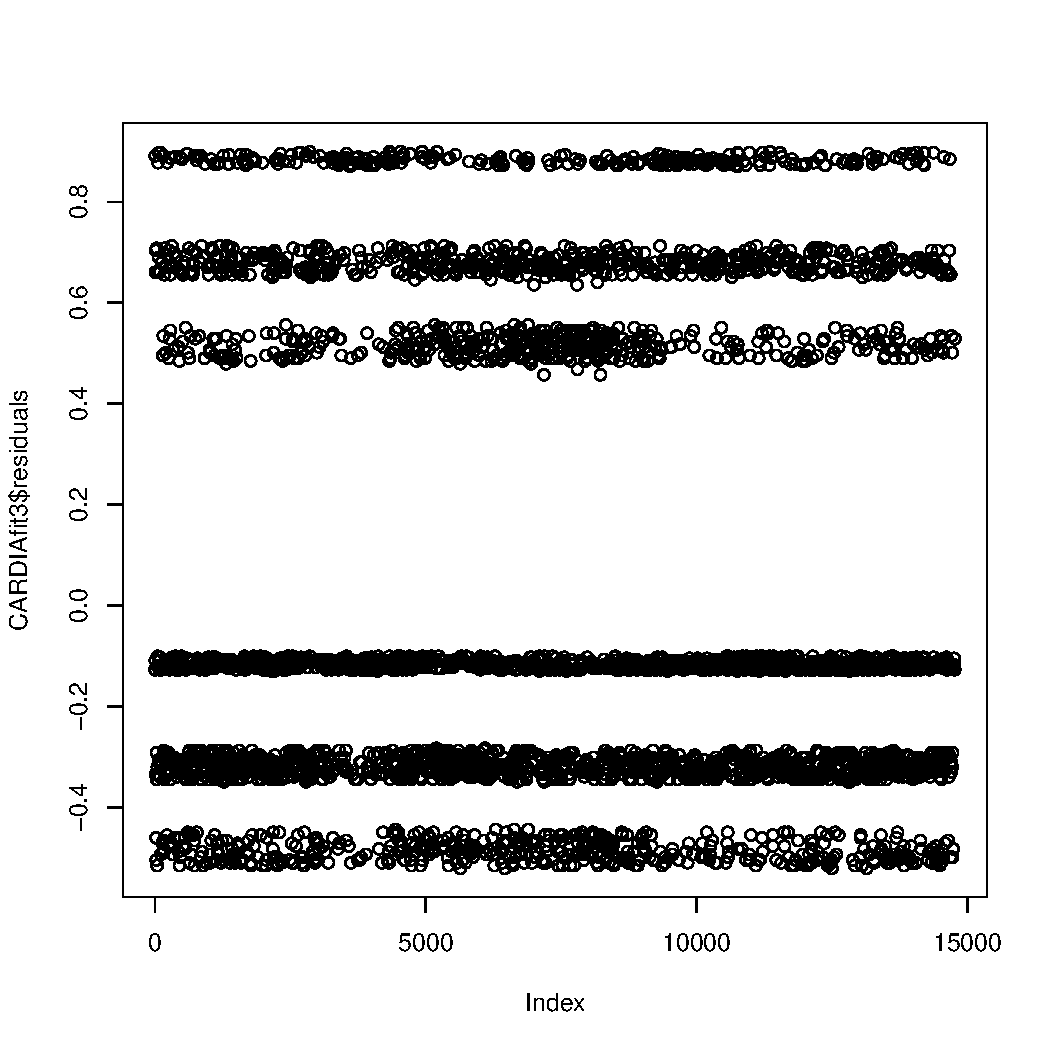
\includegraphics[width = 7cm]{figures/CARDIA3resid.pdf}  
\end{center}
\end{frame}

\subsection{Epileptic dataset}
\begin{frame}
\frametitle{Anylsis of the epileptic dataset}
Clinical trial with 59 epileptic patients, randomized to either the
anti-epileptic drug progabide or to placebo (from \citeNP{Thal:Vail:1990}).

\bs
Before treatment, the number of seizures in an eight-week period
were counted for each patient as a baseline
measurement. Is the new treatment effective at reducing the rate of sei\-zu\-res among epileptic patients?

\bs
Start with a Poisson model, but...Possible overdispersion...

\bs
  \begin{tabular}{lcccc}
\hline
\multicolumn{1}{l}{} & \multicolumn{3}{c}{Visit}\\
\hline
Treatment & 1 & 2 & 3 & 4\\
\hline
Treated & 38.7 & 16.8 & 23.8 & 18.8 \\
Placebo & 10.8 & 7.5 & 24.5 & 7.3\\
\hline
  \end{tabular}
\end{frame}


\begin{frame}
\frametitle{}
Also, the observations time are: after 8 (baseline), 10, 12, 14 and 16
weeks. Need to take into account the different length of the
observation period. We use an offset of the form $\log(t_{it})$,
where $t_{it}=8$ for the first visit and $t_{it}=2$ for the
consequent ones.

\bs
A \texttt{post} variable to account for the beginning of the study,
which takes the value 1 for visits 1, 2, 3 and 4 and the value 0 for
the baseline visit.

\bs
Allow for interaction between \texttt{post} and group.

\end{frame}

\begin{frame}[fragile]
\frametitle{}
{\tiny
\begin{lstlisting}
Call: gee(formula = y ~ post * factor(group) + offset(log(rep(c(8, 
    2, 2, 2, 2), 59))), id = Subject, data = seizure, family = poisson, 
    corstr = "exchangeable")

Coefficients:
                               Estimate Naive S.E.    Naive z Robust S.E.   Robust z
(Intercept)                  1.34760922  0.1510969  8.9188397   0.1573571  8.5640166
post                         0.11183602  0.1545145  0.7237900   0.1159304  0.9646821
factor(group)progabide       0.02753449  0.2071018  0.1329515   0.2217878  0.1241479
post:factor(group)progabide -0.10472579  0.2197052 -0.4766650   0.2134448 -0.4906459

Estimated Scale Parameter:  19.6797
Number of Iterations:  1

Working Correlation
          [,1]      [,2]      [,3]      [,4]      [,5]
[1,] 1.0000000 0.7713861 0.7713861 0.7713861 0.7713861
[2,] 0.7713861 1.0000000 0.7713861 0.7713861 0.7713861
[3,] 0.7713861 0.7713861 1.0000000 0.7713861 0.7713861
[4,] 0.7713861 0.7713861 0.7713861 1.0000000 0.7713861
[5,] 0.7713861 0.7713861 0.7713861 0.7713861 1.0000000
\end{lstlisting}
}
\end{frame}

\begin{frame}
\frametitle{}
\begin{center}
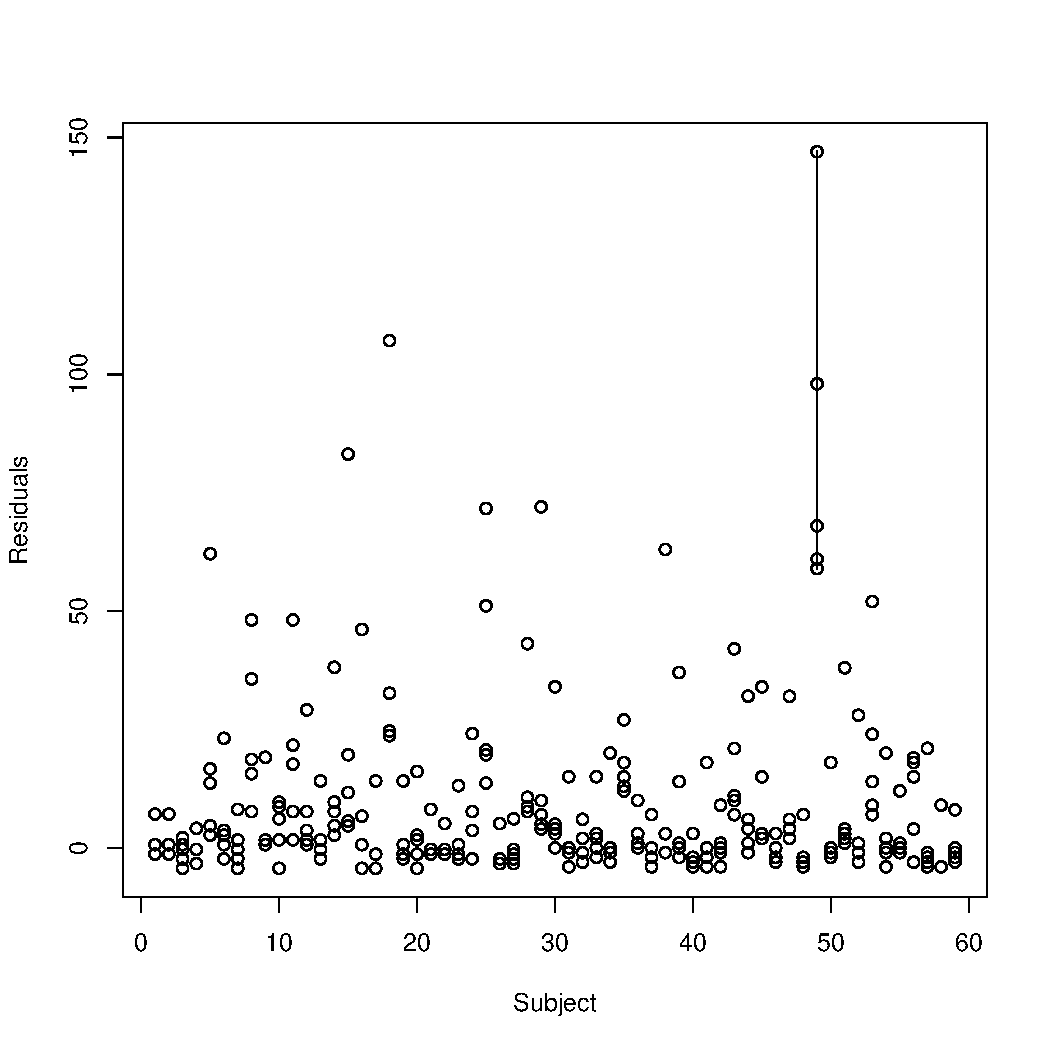
\includegraphics[width = 6.5cm]{figures/seizureresid.pdf}  
\end{center}
A very large outlier!
\end{frame}

\begin{frame}[fragile]
\frametitle{Without patient 49}
{\tiny
\begin{lstlisting}
Call: gee(formula = y ~ post * factor(group) + offset(log(rep(c(8, 
    2, 2, 2, 2), 59))), id = Subject, data = seizure, subset = Subject != 
    49, family = poisson, corstr = "exchangeable")

Coefficients:
                              Estimate Naive S.E.    Naive z Robust S.E.   Robust z
(Intercept)                  1.3476092  0.1105249 12.1928162   0.1573571  8.5640166
post                         0.1118360  0.1231346  0.9082421   0.1159304  0.9646821
factor(group)progabide      -0.1068224  0.1578051 -0.6769263   0.1936977 -0.5514904
post:factor(group)progabide -0.3023841  0.1933863 -1.5636272   0.1710601 -1.7677071

Estimated Scale Parameter:  10.52997
Number of Iterations:  1

Working Correlation
         [,1]     [,2]     [,3]     [,4]     [,5]
[1,] 1.000000 0.593689 0.593689 0.593689 0.593689
[2,] 0.593689 1.000000 0.593689 0.593689 0.593689
[3,] 0.593689 0.593689 1.000000 0.593689 0.593689
[4,] 0.593689 0.593689 0.593689 1.000000 0.593689
[5,] 0.593689 0.593689 0.593689 0.593689 1.000000
\end{lstlisting}
}

Large differences in (some) estimated parameters and standard
errors!
\end{frame}

\section{Generalized linear mixed models (GLMM)}
\label{GLMM.section}

\subsection{Model definition}
\begin{frame}
\frametitle{Generalized linear mixed models (GLMM)}
With longitudinal/clustered data one need to take into account the within
cluster correlation. 

\bs 

GLM is not adequate. GLMM extends GLM by allowing coefficients to vary with
cluster, allowing for within cluster correlation.

\bs
GLMM is a compromise between the GLM population-average model and a
(over-pa\-ra\-metrized) modelling approach that would fit each cluster separately.
\end{frame}

\begin{frame}
\frametitle{}
Ingredients:
\begin{itemize}
\item response vectors $Y_i = (Y_{i1},\ldots,Y_{in_i})$, for $i=1,\ldots,n$.
\item design matrix $X_i$ for the fixed effects
\item design matrix $Z_i$ for the random effects (possibly overlapping with
$X_i$). 
\item random effects $\gamma_i$ for each cluster $i$. These are latent (non-observed) random variables.
\end{itemize}

\bs
Assumptions:
\begin{itemize}
\item $Y_{it} \mid \gamma_i$ are independently distributed according to a
  distribution from the exponential family.
\item $\gamma_i$ are independently distributed according to ${\mathcal
    N}(0, \Psi)$. 
\end{itemize}

\bs
Two sources of error: the sampling process and the measurement process
within the sample itself.
\end{frame}

\begin{frame}
\frametitle{The Gaussian-identity link case}
In the Gaussian-identity link case, the model can be written as:
$$ Y_i = X_i \beta + Z_i \gamma_i + \epsilon_i \ \ \  (\mbox{or } Y_{it} = x_{it}^T \beta + z_{it}^T \gamma_i + \epsilon_{it}),$$
with $\epsilon_i \sim {\mathcal N}(0, \sigma^2_{\epsilon} I)$ and $\gamma_i  \sim
{\mathcal N}(0,\Psi)$, for example $\Psi = \sigma^2_{\gamma} I$.

\bs
Equivalently: $E(Y_i \mid \gamma_i) = X_i \beta + Z_i \gamma_i$.


\bigskip

It follows that
$$Y_i \sim {\mathcal N}(X_i \beta, Z_i \Psi Z_i^T + \sigma^2_{\epsilon} I),$$
and the (log-)likelihood can be written explicitly for this
multivariate normal distribution (but still needs an optimization
algorithm because of the parameters in $\Psi$).
\end{frame}

\begin{frame}
\frametitle{}

\begin{center}
\begin{tabular}{cc} 
Random intercept model & Random slope model \\
$Y_{it} = x_{it}^T \beta + \gamma_i + \epsilon_{it}$ & $Y_{it} = x_{it}^T \beta + z_{it}^T \gamma_i + \epsilon_{it}$\\
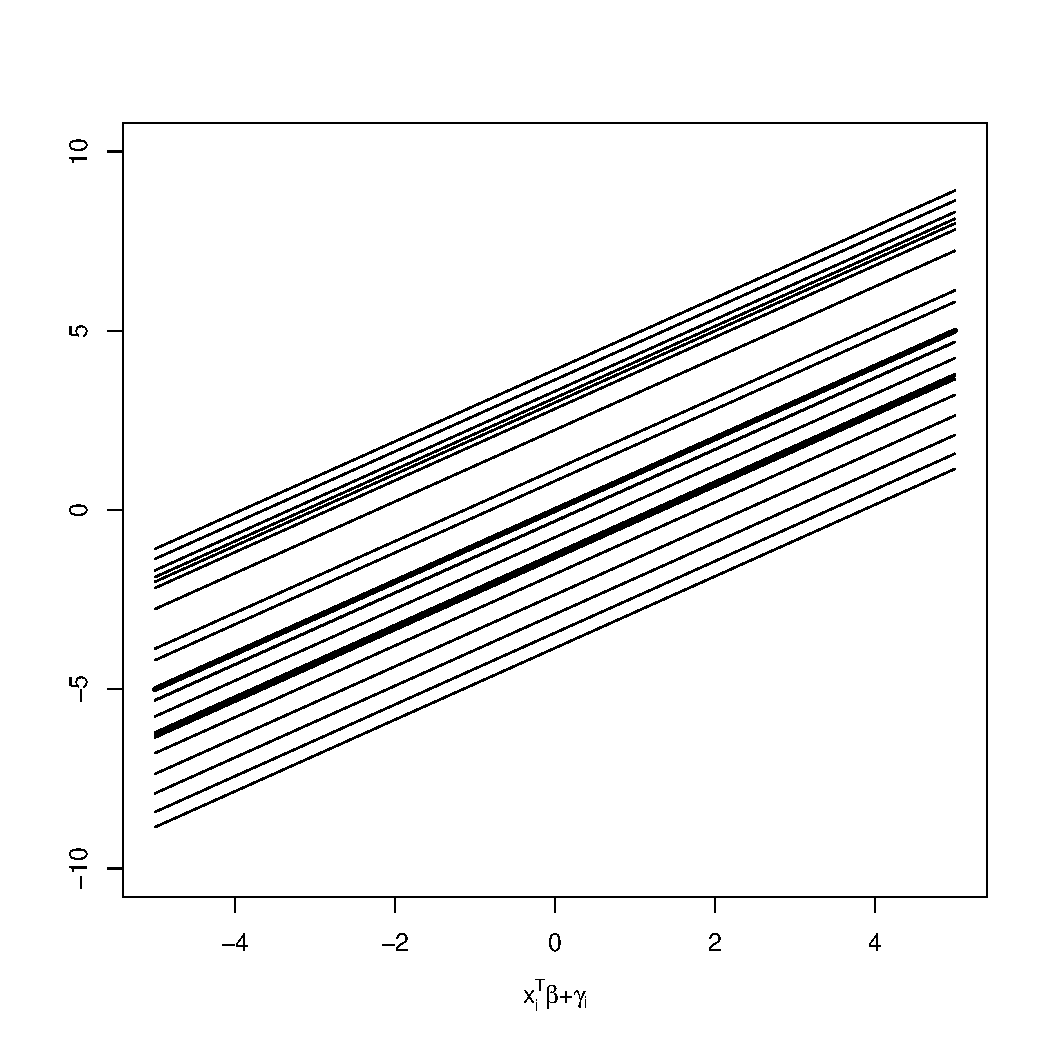
\includegraphics[width = 5.5cm]{figures/RandomInterceptGaussian.pdf}  & 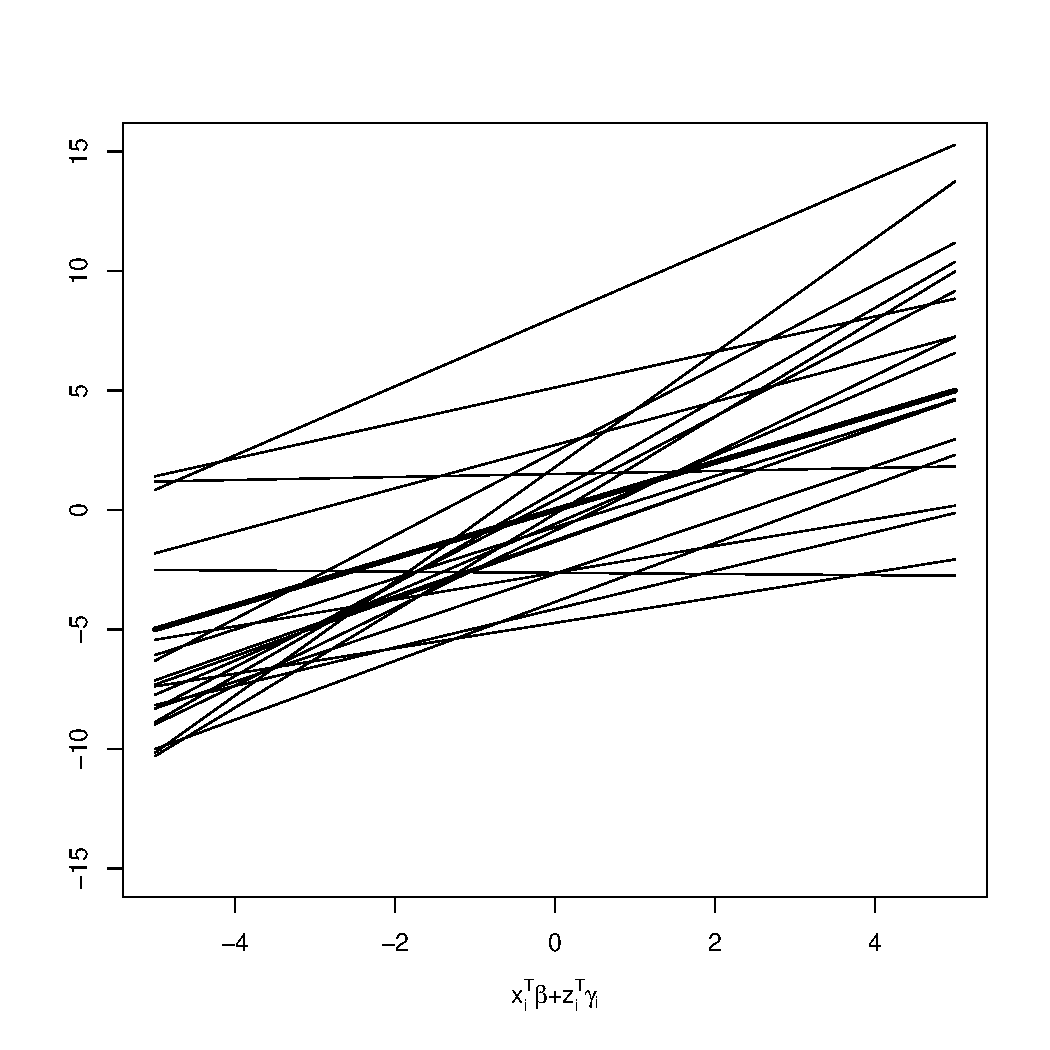
\includegraphics[width =5.5cm]{figures/RandomSlopeGaussian.pdf} 
\end{tabular}
\end{center}


\end{frame}

\begin{frame}
\frametitle{The generalized linear mixed model}

\bs
Denote $\mu_{it} = E(Y_{it} \mid \gamma_i)$ ($\neq E(Y_{it})$).

\bs
Model (conditional on $\gamma_i$, a standard GLM):
\begin{itemize}
\item $g(E(Y_{it} \mid \gamma_i)) = g(\mu_{it}) =  x_{it}^T \beta + z_{it}^T \gamma_i$
  for a link function $g$. 
\item $Var(Y_{it} \mid \gamma_i) = v(\mu_{it})$.
\end{itemize}

\bs
Two sources of error: the sampling process and the measurement process
within the sample itself.
\end{frame}

\begin{frame}
\frametitle{Estimation of GLMM}

Combine the information from
\begin{itemize}
\item the conditional distribution of $Y_{it}
\mid \gamma_i$: $f(y_{it} \mid \gamma_i, \beta, \phi)$;
\item the marginal distribution of the random effects: $f(\gamma_i \mid
\phi, \Psi)$. 
\end{itemize}

\bs
The $\gamma_i$ are unobservable, we rely on the marginal likelihood: 
\begin{eqnarray*}
\lefteqn{L(\beta,\phi, \Psi) = f(y_1,\ldots,y_n)= \prod_{i=1}^n f(y_i) }\\
& = & \prod_{i=1}^n \int \cdots \int f(y_{i} \mid \gamma_i, \beta, \phi)f(\gamma_i \mid \phi, \Psi) d \gamma_i  \\
& = & \prod_{i=1}^n \int \cdots \int \prod_{t=1}^{n_i} f(y_{it} \mid \gamma_i,
\beta, \phi) f(\gamma_i \mid \phi, \Psi) d \gamma_i.
\end{eqnarray*}

As in GLM, use the model relationship to introduce the data information.

\end{frame}

\begin{frame}
\frametitle{Approximations of $L(\beta,\phi, \Psi)$}

The likelihood cannot -- in general -- be expressed in closed form.
Numerical methods and approximations to compute/approximate the integrals are needed:
\begin{itemize}
\item Monte-Carlo integrations (MCMC) (approximate the integrals by simulation)
\item Gauss-Hermite quadrature approximation
\item Laplace approximation
\item Penalized Quasi-Likelihood (PQL)
\item Marginal Quasi-Likelihood (MQL)
\end{itemize}

\bs
Note: PQL and MQL can produce biased estimators. Better to use Gaussian
quadrature or Laplace approximation, even if they can be computationally quite
intensive. 

\bs
For elaborate specifications of random effects, the only effective
integration schemes seem to be those based on MCMC.

\end{frame}

\begin{frame}
\frametitle{Some available options in R}

\begin{itemize}
\item package \texttt{nlme}: functions \texttt{lme} and  \texttt{nlme}
  for  linear and nonlinear mixed effects models. Allow for nested
  random effects. 
\item package \texttt{lme4}: function \texttt{lmer}. Allows Laplace approximation (default) and adaptive
Gaussian quadrature approximation. Can define random
intercepts and random slopes, as well as nested and crossing grouping
factors for random effects. 
\item package \texttt{ADMB}: function \texttt{glmmadmb} based on a Laplace
approximation with automatic differentiation. Wide range of families,
wide range of link functions, single or multiple random effects, including both
nested and crossed effects.
\item package \texttt{glmmTMB}, function \texttt{glmmTMB}. Similar to \texttt{glmmadmb}, but some different extensions.
\end{itemize}

\end{frame}


\begin{frame}
\frametitle{Interpretation of the fixed effects}
A GLMM is a subject specific analysis: the regression coefficients
apply to each individual, but not necessarily to the population (in
contrast to a marginal analysis, e.g.\ GEE).

\bs
We have that:
$$\mu_{it} = E(Y_{it}\mid \gamma_i) = g^{-1}(x_{it}^T \beta + z_{it}^T \gamma_i),$$
so that the conditional mean varies with the predictors according 
to $\beta$ with in addition a subject specific contribution due to $\gamma_i$.

\end{frame}

\begin{frame}
\frametitle{}
The population mean $E(Y_{it})$ is defined by
$$E(Y_{it}) = E_{\gamma_i}(E(Y_{it}\mid \gamma_i)) = \int g^{-1}(x_{it}^T \beta + z_{it}^T
\gamma_i) dF(\gamma_i),$$
which is different from $g^{-1}(x_{it}^T \beta)$, except in the
Gaussian-identity link case. 

\bs
In some cases (e.g.\ the probit model) it holds that
$$E(Y_{it}) = E_{\gamma_i}(E(Y_{it}\mid \gamma_i)) = g^{-1}(x_{it}^T \beta^*),$$
with $\mid \beta^* \mid \leq  \mid \beta \mid$. 
\end{frame}

\begin{frame}
\frametitle{}
\begin{center}
\begin{tabular}{cc} 
Random intercept model & Random slope model \\
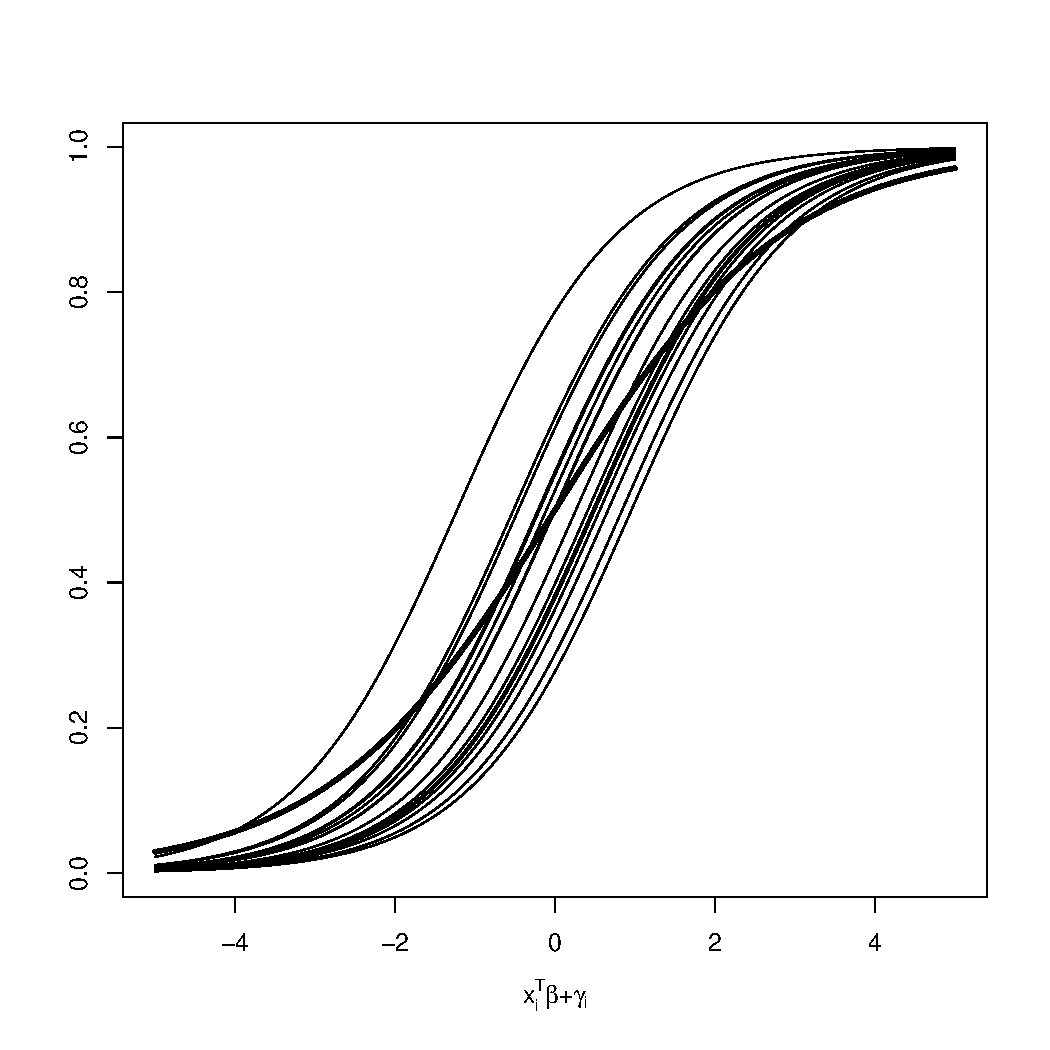
\includegraphics[width = 5.5cm]{figures/RandomIntercept.pdf}  & 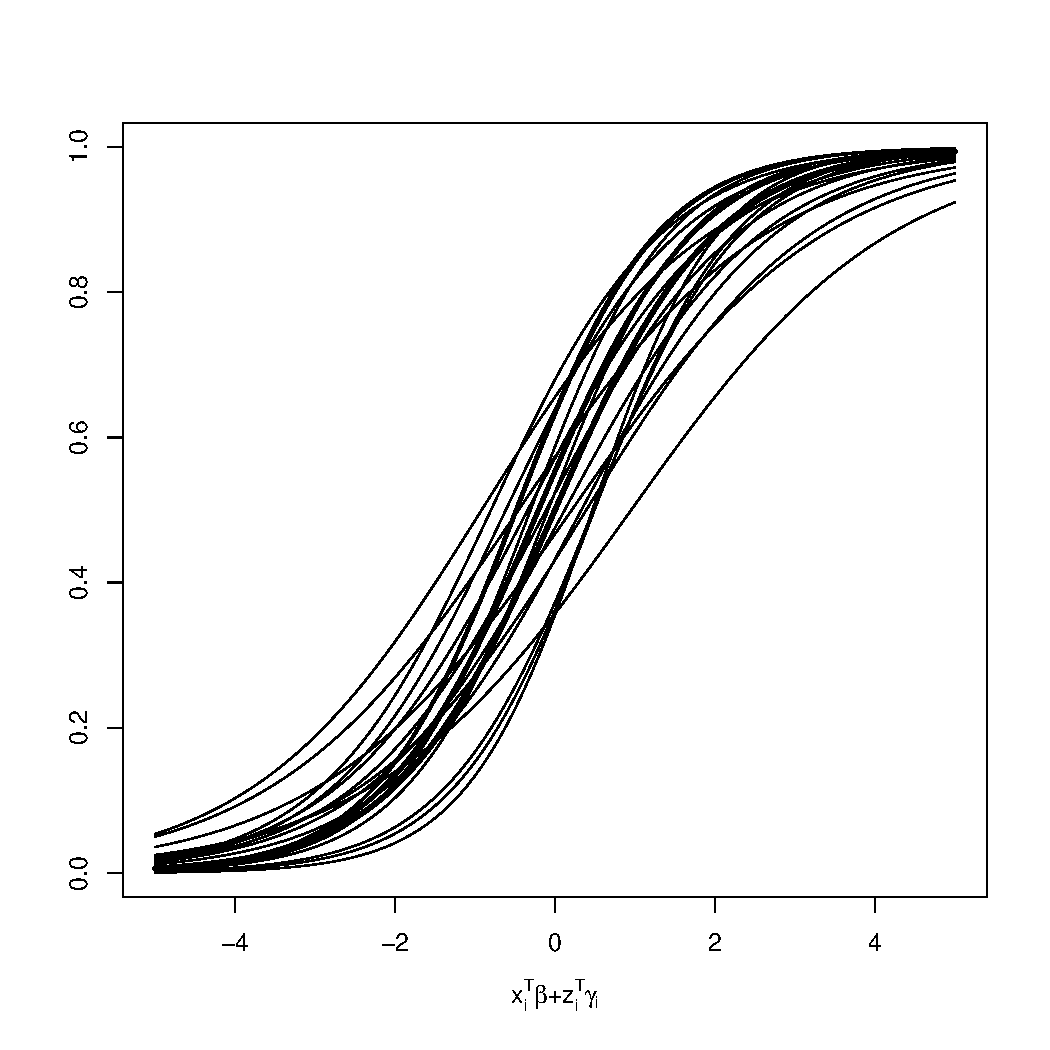
\includegraphics[width =5.5cm]{figures/RandomSlope.pdf} 
\end{tabular}
\end{center}

\end{frame}

\begin{frame}
\frametitle{Prediction of the random effects}
For linear mixed models theory exists to define BP (best predictors minimizing
MSE, $\hat{\gamma}_i = E(\gamma_i \mid y_i) $), BLP (best linear
predictors) and BLUE (best linear unbiased predictors). They all go
down to the same. 

\bs
In GLMM software, usually the conditional modes are implemented, that is the
values maximising the density of $\gamma_i \mid y_1, \ldots, y_n$. They are not
BLUP, because they are not linear, they might not be unbiased and we don't know
in which sense they are best.

\bs
The best predictors would be the one satisfying
$\hat{\gamma}_i = E(\gamma_i \mid y_i) $. Still an open field of research (in
particular to define the properties of $\hat{\gamma}_i$). 
\end{frame}

\begin{frame}
\frametitle{}
In fact, the question to ask is what is the prediction for:
\begin{itemize}
\item a new data point in an existing group: use $\hat{\mu}_{it} = g^{-1}(x_{it}^T \hat{\beta} + z_{it}^T \hat{\gamma}_i)$; 
\item a new data point for a new group: use $\hat{\mu}_i = g^{-1}(x_{it}^T
\hat{\beta})$. 
\end{itemize}
\end{frame}

\subsection{Pseudoneglect dataset}
\begin{frame}
\frametitle{Analysis on data on the pseudoneglect}

The effects of hemispace on a tactile line bisection task are measured. Data come from a diploma thesis (Sabina Catalano, FAPSE, 2003). We have observations on 10 subjects measured 10 times for each of 13th distances (from 0 to 120, 60 being the center of the line).  The subject is presented (in a random sequence) with a position on a line and has to decide whether it lies on the left or on the right of the center. The number of "left" answers (for each distance) is recorded.

In this experiment the scientific question is to see whether there is a systematic bias to the left from the center
line (as suggested by some psychologists). 

\bs
The "equality subjective point" (ESP), i.e. the distance 
for  which the probability of "left" is 1/2, is the parameter of interest.
\end{frame}

\begin{frame}
\frametitle{}
\begin{center}
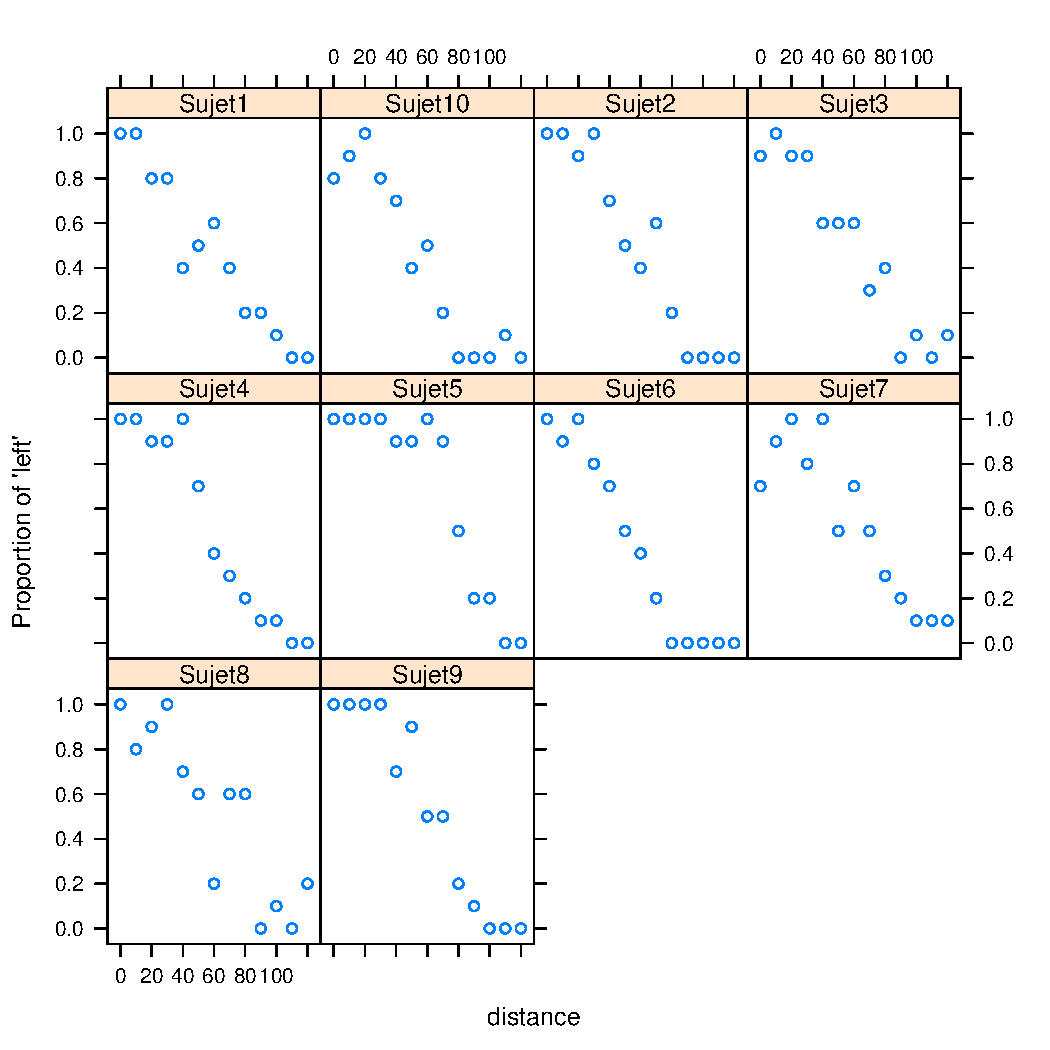
\includegraphics[width = 7.5cm]{figures/hemiID.pdf}  
\end{center}

\end{frame}

\begin{frame}
\frametitle{Average over individuals}

\begin{center}
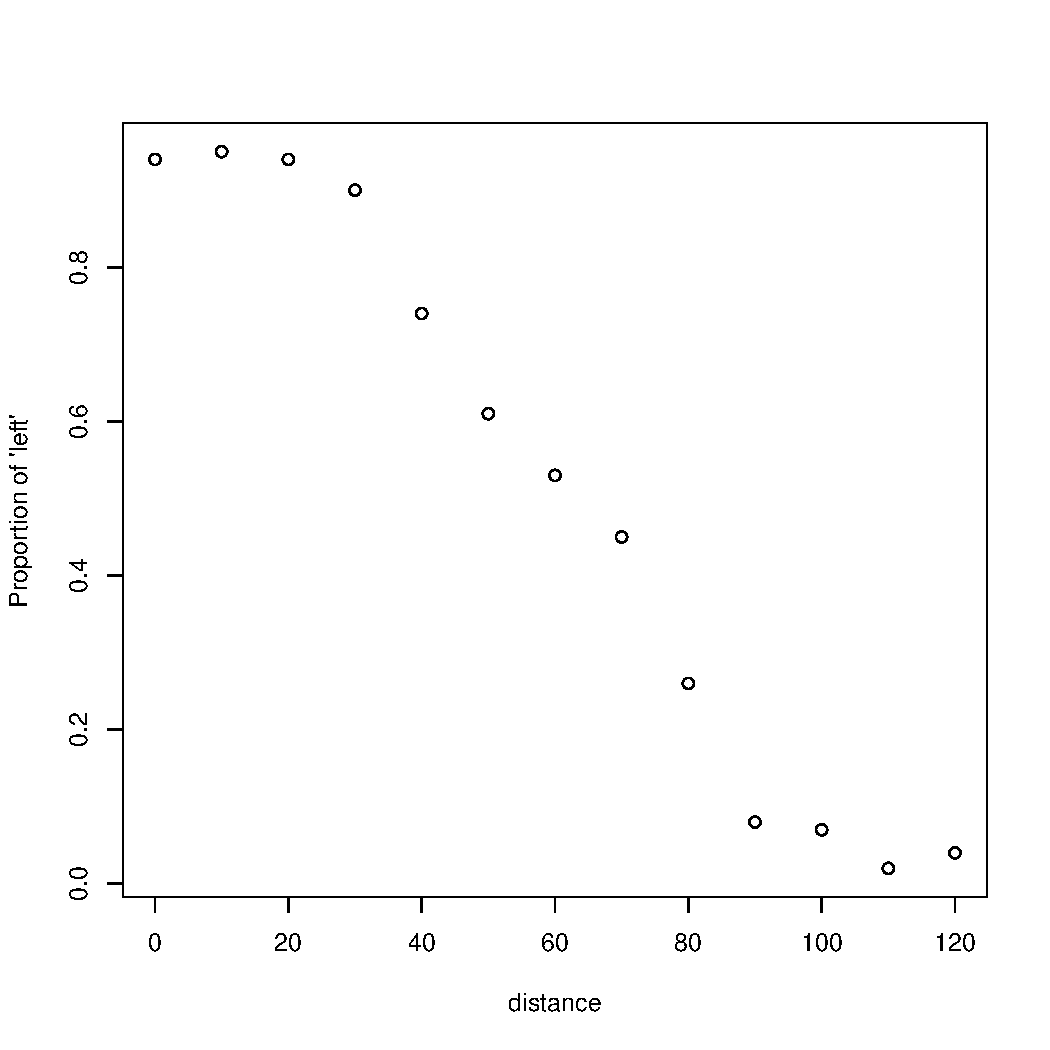
\includegraphics[width = 7cm]{figures/hemi.pdf}  
\end{center}
\end{frame}

\begin{frame}
\frametitle{}
We consider a binomial GLMM model with random intercept:

$$\mbox{logit}(p_i) = \log\Big( \frac{p_i}{1-p_i}\Big) = \beta_0 + \beta_1 \texttt{distance} + \gamma_i,$$
with $p_i = P(\mbox{"left" for individual }i)$ and $\gamma_i \sim {\mathcal N}(0,\sigma_{\gamma}^2)$ is a random intercept.

\bs
\bs
\bs
For each individual, the ESP is the distance such that
$$ \beta_0 + \beta_1 \texttt{distance} + \gamma_i =0,$$

that is
$$ ESP_i = - \frac{\beta_0 + \gamma_i}{\beta_1}.$$
\end{frame}


\begin{frame}[fragile]
\frametitle{}
{\tiny
\begin{lstlisting}
Generalized linear mixed model fit by maximum likelihood (Laplace Approximation) ['glmerMod']
 Family: binomial  ( logit )
Formula: cbind(left, 10 - left) ~ distance + (1 | sujet)
   Data: hemi

     AIC      BIC   logLik deviance df.resid 
   371.4    380.0   -182.7    365.4      127 

Scaled residuals: 
    Min      1Q  Median      3Q     Max 
-6.6927 -0.6634 -0.1685  0.6606  3.5747 

Random effects:
 Groups Name        Variance Std.Dev.
 sujet  (Intercept) 0.2469   0.4969  
Number of obs: 130, groups:  sujet, 10

Fixed effects:
             Estimate Std. Error z value Pr(>|z|)    
(Intercept)  3.804820   0.264566   14.38   <2e-16 ***
distance        -0.063078   0.003267  -19.31   <2e-16 ***
---
Signif. codes:  0 ‘***’ 0.001 ‘**’ 0.01 ‘*’ 0.05 ‘.’ 0.1 ‘ ’ 1

Correlation of Fixed Effects:
     (Intr)
distance -0.744
\end{lstlisting}
}
\end{frame}

\begin{frame}
\frametitle{}
With caution:
\begin{center}
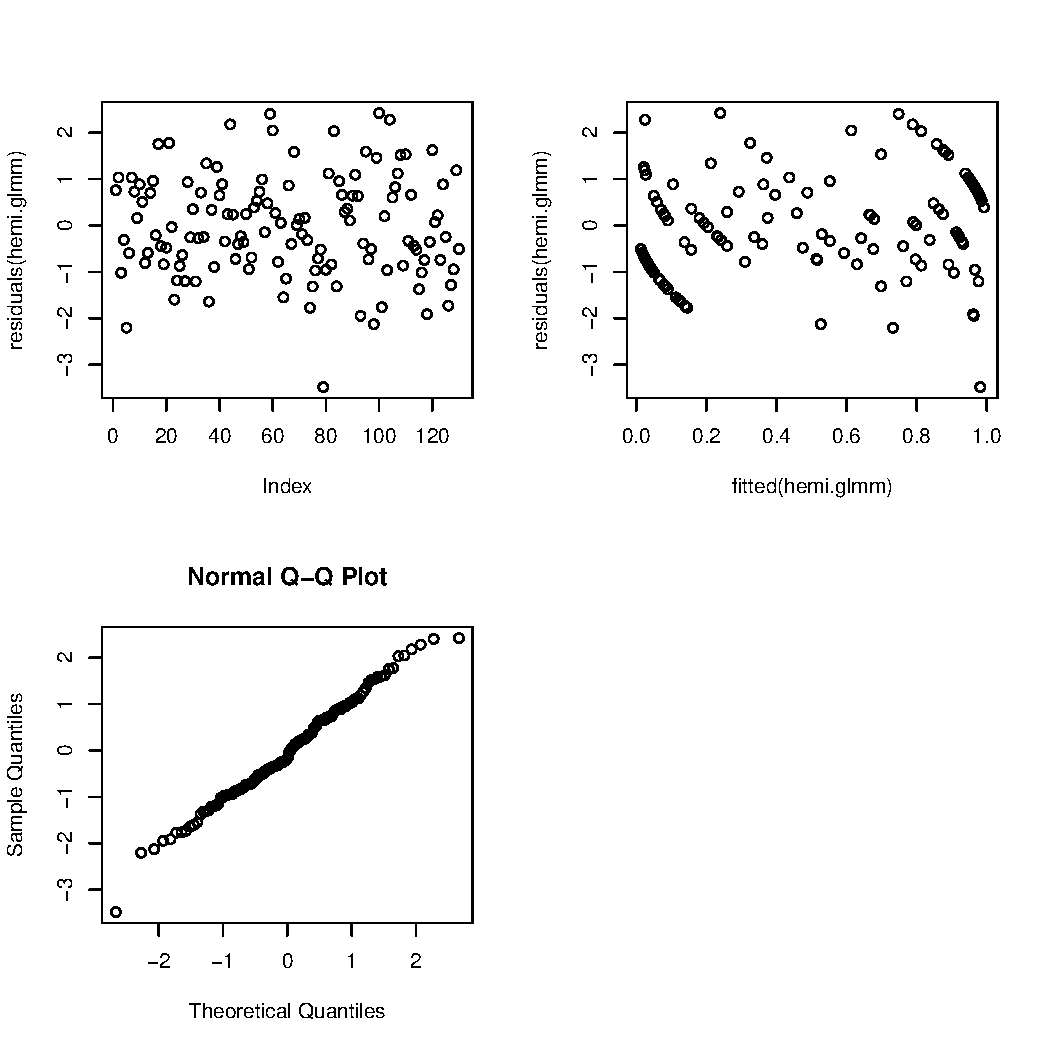
\includegraphics[width = 7cm]{figures/hemires.pdf}  
\end{center}
\end{frame}


\begin{frame}[fragile]
\frametitle{}
Are the random effects worth the trouble? Comparison with a GLM fit (which is nested within a GLMM model):

{\tiny
\begin{lstlisting}
Call: glm(formula = cbind(gauche, 10 - gauche) ~ item, family = binomial, 
    data = hemi)

Deviance Residuals: 
    Min       1Q   Median       3Q      Max  
-3.1932  -0.9789  -0.2511   0.9206   3.6980  

Coefficients:
             Estimate Std. Error z value Pr(>|z|)    
(Intercept)  3.650109   0.202573   18.02   <2e-16 ***
item        -0.060521   0.003093  -19.57   <2e-16 ***
---
Signif. codes:  0 ‘***’ 0.001 ‘**’ 0.01 ‘*’ 0.05 ‘.’ 0.1 ‘ ’ 1

(Dispersion parameter for binomial family taken to be 1)

    Null deviance: 988.40  on 129  degrees of freedom
Residual deviance: 198.04  on 128  degrees of freedom
AIC: 390.75

Number of Fisher Scoring iterations: 5
\end{lstlisting}
}

\bs
In GLMM: AIC=371.4 and the deviance=365.4. 
\end{frame}




\begin{frame}[fragile]
\frametitle{Prediction of ESP}

{\tiny
\begin{lstlisting}
-(fixef(hemi.glmm)[1] +ranef(hemi.glmm)$sujet)/fixef(hemi.glmm)[2]
        (Intercept)
Sujet1     55.97849
Sujet10    51.06305
Sujet2     58.43176
Sujet3     59.24924
Sujet4     60.88410
Sujet5     77.32295
Sujet6     51.88350
Sujet7     63.33696
Sujet8     61.70159
Sujet9     63.33696
\end{lstlisting}
}

\vspace*{-2cm}
\begin{center}
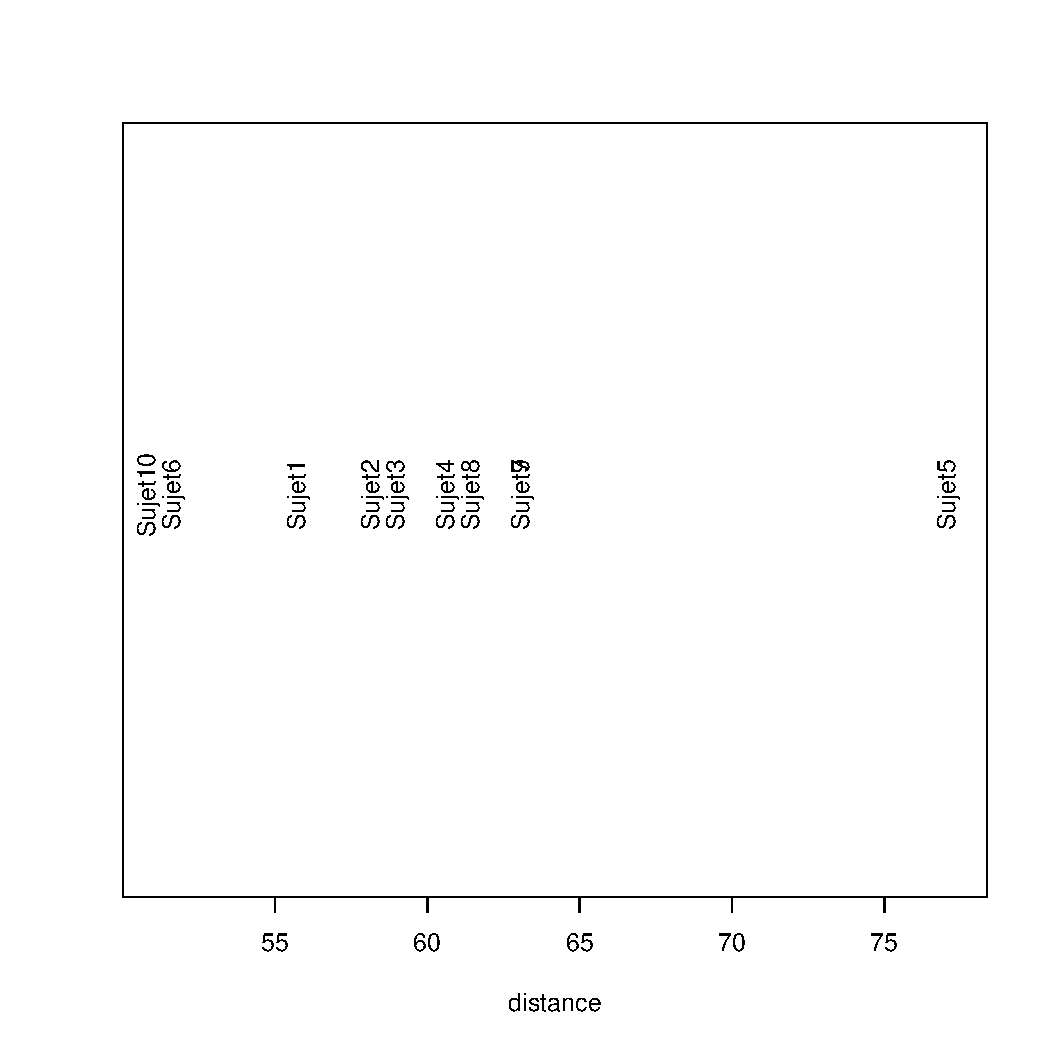
\includegraphics[width = 6cm]{figures/ESP.pdf}  
\end{center}
\end{frame}


\begin{frame}[fragile]
\frametitle{With random slope?}

{\tiny
\begin{lstlisting}
Generalized linear mixed model fit by maximum likelihood (Laplace Approximation) ['glmerMod']
 Family: binomial  ( logit )
Formula: cbind(left, 10 - left) ~ item + (1 + distance | sujet)
   Data: hemi

     AIC      BIC   logLik deviance df.resid 
   368.4    382.8   -179.2    358.4      125 

Scaled residuals: 
    Min      1Q  Median      3Q     Max 
-3.8813 -0.5607 -0.0854  0.5181  2.3284 

Random effects:
 Groups Name        Variance  Std.Dev. Corr 
 sujet  (Intercept) 1.2714312 1.12758       
        distance    0.0001859 0.01363  -0.87
Number of obs: 130, groups:  sujet, 10

Fixed effects:
            Estimate Std. Error z value Pr(>|z|)    
(Intercept)  4.02204    0.43108    9.33   <2e-16 ***
distance    -0.06629    0.00565  -11.73   <2e-16 ***
---
Signif. codes:  0 ‘***’ 0.001 ‘**’ 0.01 ‘*’ 0.05 ‘.’ 0.1 ‘ ’ 1

Correlation of Fixed Effects:
     (Intr)
item -0.885
\end{lstlisting}
}
\end{frame}
\section{Robust GLM}
\label{robust.section}

\subsection{Introduction}
\begin{frame}
\frametitle{Robust statistics}

Statistical analyses can be very much affected by outliers. We do not want the
analysis (and therefore the conclusions) to be driven by a single or very few
observations.

\bs
Rather: model the majority (bulk) of the data.

\bs
With the {\color{blue}robust statistics} approach (\citeN{Hube:1981} and
\citeN{Hamp:Ronc:Rous:Stah:1986}) we consider that:
\begin{itemize}
\item models are at best ideal approximations of the underlying process
\item deviations from the distributional assumptions are (almost) always
present in real data.
\end{itemize}
\end{frame}

\begin{frame}
\frametitle{}
Basic idea: assume that the distribution of the data comes from a
{\color{blue}neighborhood of the postulated model}.

\bs
Construct robust estimators (and test statistics) such that the estimated
parameters (inferences) are consistent at the postulated model and stable in a
neighborhood of it.

Correct estimation and inference is obtained for the parameters of the
postulated model (the one corresponding to the {\color{blue}majority of the
data}) by limiting
the influence of (a small fraction of) data points which are thought of as
coming from a different population.
\end{frame}

\begin{frame}
\frametitle{}
The {\color{blue}stability} of the robust technique is achieved at the price of
a slight loss of {\color{blue}efficiency} at the model. This can be viewed as an
insurance premium one is willing to pay to protect against biases and losses of
efficiency due to deviations from the assumed model.

\begin{center}
{\LARGE{\color{blue}Robust statistics, as a collection of related theories, is
the statistics of approximate parametric models.}}
\end{center}

\bs

from \citeN{Hamp:Ronc:Rous:Stah:1986}, p.~7.
\end{frame}

\begin{frame}
\frametitle{}
{\color{blue}Neighborhood of the postulated model}:
$F_{\epsilon} = (1-\epsilon) F_{\theta} + \epsilon G,$
where $F_{\theta}$ is the postulated model, $\theta$ is a set of parameters of
interest, $G$ is an arbitrary distribution and $0\leq \epsilon \leq 1$.

\begin{table}[h]
{\scriptsize\begin{tabular}{lccc}
 Inference & \multicolumn{3}{c}{Classical} \\ \hline\\
 $G$ &
$0<<\varepsilon <1$ & $0<\varepsilon <<1$ & $\varepsilon =0$ \\
\hline \\
arbitrary & ? & ? & $F_{\theta }$ \\
$G=\Delta _{z}$ & $F_{\varepsilon }$ & $F_{\varepsilon }$ & $F_{\theta }$ \\
$G=F_{(\theta ,\theta ^{\prime })}$ & $F_{\varepsilon }$ &
$F_{\varepsilon }$
& $F_{\theta }$ \\
$G$ such that $F_{\varepsilon }=F_{(\theta ,\theta ^{\prime })}$ & $%
F_{(\theta ,\theta ^{\prime })}$ & $F_{(\theta ,\theta ^{\prime })}$ & $%
F_{\theta }$ \\ \hline\\
 & \multicolumn{3}{c}{Robust} \\ 
\hline \\
arbitrary & ? & $F_{\theta }$ & $F_{\theta }$ \\
$G=\Delta _{z}$ & $F_{\varepsilon }$ & $F_{\theta }$ & $F_{\theta }$ \\
$G=F_{(\theta ,\theta ^{\prime })}$ & $F_{\varepsilon }$ & $F_{\theta }$ & $%
F_{\theta }$ \\
$G$ such that $F_{\varepsilon }=F_{(\theta ,\theta ^{\prime })}$ & $%
F_{(\theta ,\theta ^{\prime })}$ & $F_{\theta }$ & $F_{\theta }$ \\
\hline
\end{tabular}}
\end{table}

Table from \citeN{Heri:Cant:Copt:Vict:2009}.
\end{frame}

\begin{frame}
\frametitle{Tools to measure robustness}
\begin{itemize}
\item{\color{blue}Influence function} defined by
$$IF({\bf z}; T , F) = \lim_{\epsilon \rightarrow 0} \Big(\frac{T(F_{\epsilon}) -
  T(F)}{\epsilon} \Big),$$
where $T(F)$ is a functional that defines the estimator $T(F^{(n)})$, $F^{(n)}$
is the empirical distribution function, $F_{\epsilon} = (1-\epsilon) F +
\epsilon \Delta_{\bf z}$, and $\Delta_{\bf z}$ is a distribution that puts all
its mass at ${\bf z}$.

$IF$ measures the effect on the estimate of an infinitesimal contamination at
the point ${\bf z}$, standardized by the amount of contamination. The maximal
marginal effect of an observation {\bf z} on T is approximately $\epsilon \cdot
IF({\bf z}; T , F)$.

A  {\color{blue}bounded influence function} is a desirable property for an
estimator.
\end{itemize}
\end{frame}


\begin{frame}
\frametitle{}
\begin{itemize}
\item {\color{blue}Breakdown point} It measures the maximum permitted
percentage of the minority such that it has only limited influence on the
estimator. The {\color{blue}larger} the breakdown point, the more robust the
estimator.
\end{itemize}
\end{frame}

\begin{frame}
\frametitle{Robust statistics versus diagnostic?}

\bs
Why not performing diagnostic to identify outlying observations on the basis of
a classical analysis and then remove the unusual data points from the
sample?

\bs
Can be unreliable because a {\color{blue}masking effect} can occur,
where a single large outlier may mask others. This means that the distorted data
appear to be the norm rather than the exception.


\bs
Removal of outlying points base on a classical analysis is a binary decision (in
or out), whereas the robust approach is a smoother process.

\bs
If the removal approach is used, the subsequent inference should take it into
account (often not the case).
\end{frame}


\begin{frame}
\frametitle{M-estimation}
A large number of estimators fall in the class of M-estimators defined by
\citeN{Hube:1964}. To estimate a parameter $\theta$,for a given function $\Psi$,  they are defined by the
estimating equations:
$$\sum_{i=1}^n \Psi(y_i,\theta) = 0.$$

Under certain regularity conditions:
\begin{itemize}
\item $\sqrt{n} (\hat{\theta} - \theta)$ is asymptotically normally distributed
with mean 0 and variance $\Omega = M^{-1} Q M^{-1}$, where $M=- E(d/ d \theta
\Psi(y,\theta))$ and $Q= E (\Psi(y,\theta) \Psi^T(y,\theta))$.
\item the influence function of an M-estimator is $M^{-1} \Psi(y,\theta)$, that is
proportional to $\Psi(y,\theta)$.
\end{itemize}

\end{frame}

\begin{frame}
\frametitle{Example}

The {\color{blue} ML estimator for GLM} (p.~\pageref{EE.GLM}) is
an M-estimator with 
$$\Psi(y_i,\mu_i) = \frac{y_i-\mu_i}{Var(Y_i)} x_{ij}
(\frac{\partial \mu_i}{\partial \eta_i}) = \frac{r_i}{v^{1/2}(\mu_i)} \mu_i^{\prime}.$$

\bs
This function is unbounded with respect to $y_i$ and with respect to $x_i$. The
GLM estimator is {\color{blue}not robust}!

\end{frame}

\subsection{Robust GLM estimator}
\begin{frame}
\frametitle{Robust GLM estimator}
Introduce a function $\psi$ to control 
large deviations in the $y$-space and a set of weights  $w({\bf x}_i)$ to
downweight leverage points:
\begin{equation*}
\label{EE.eq}
\sum_{i=1}^n \Big[ \psi(r_i ) w({\bf x}_i)
\frac{1}{v^{1/2}(\mu_i)}  \mu_i^{\prime}  - a(\beta) \Big] = {\bf 0},
\end{equation*}
where $r_i = (y_i-\mu_i)/v^{1/2}(\mu_i)$ are the Pearson residuals \cite{Cant:Ronc:2001a}.

\bs
The correction term $a(\beta)$ ensures Fisher consistency.

\bs
The classical estimating equations are a special case: $\psi$
is the identity function and $ w({\bf x}_i) \equiv 1$,
in which case it holds that $a(\beta) = 0$.
\end{frame}


\begin{frame}
\frametitle{}
The set of estimating equations for robust GLM can be rewritten as :
\begin{equation*}
\label{EEw.eq}
\sum_{i=1}^n \Big[ \tilde{w}(r_i) r_i w({\bf x}_i)
\frac{1}{v^{1/2}(\mu_i)}  \mu_i^{\prime}  - a(\beta) \Big] = {\bf 0},
\end{equation*}
where $\tilde{w}(r) = \psi(r)/r$.
\label{EEw.page}

\bs
Interpretation: these are GLM estimating equations weighted to ensure robustness
and recentered to ensure consistency.
\end{frame}

\begin{frame}
\frametitle{Choices for $\psi$}
A common choice for $\psi$ to ensure robustness is the so-called Huber's
function defined by $\psi_c(r) = r \cdot \min(1, c/|r|)$. 

\bs
$c$ allows the tuning
of the robustness-efficiency compromise. (In practice, take $c$ between 1
and 2).

\begin{center}
\begin{tabular}{cc}
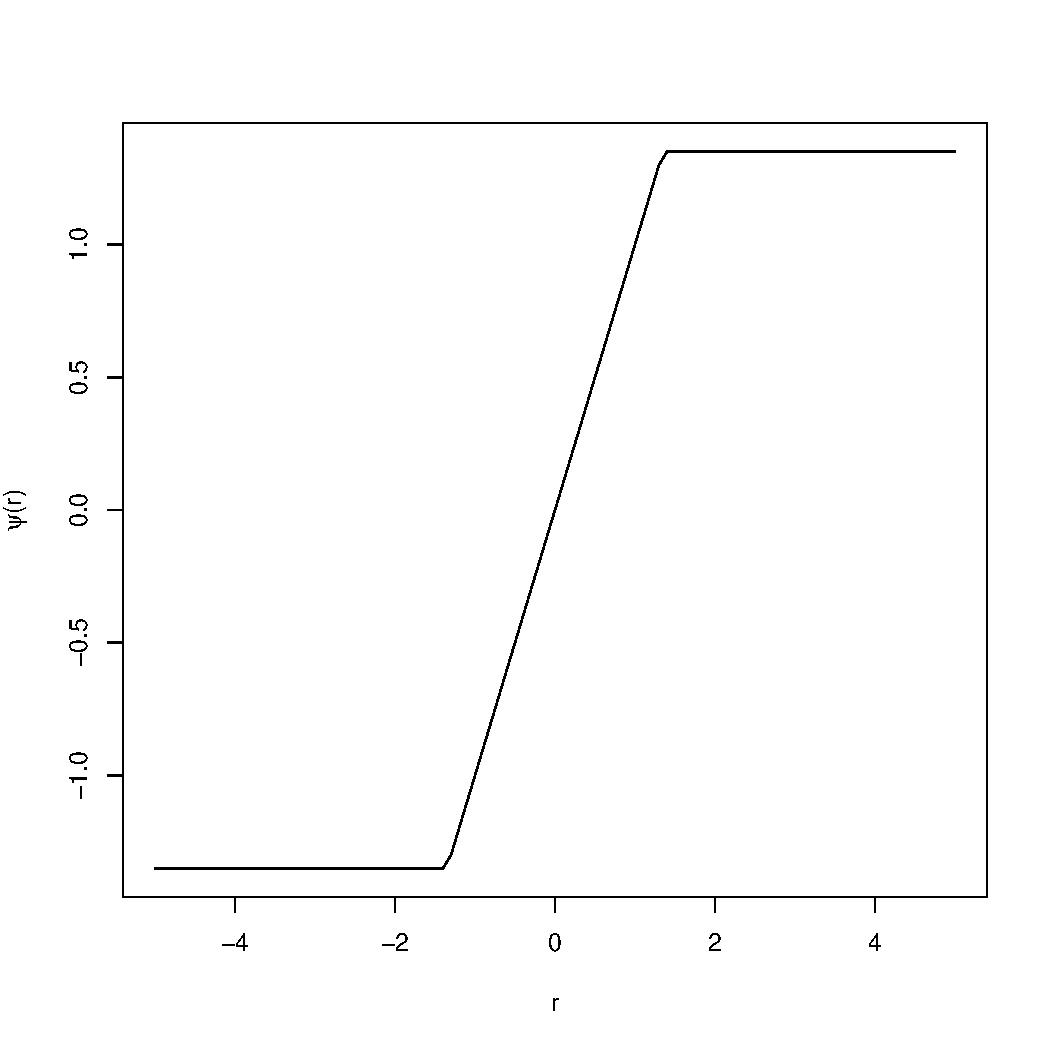
\includegraphics[width = 4.5cm]{figures/Huberpsi.pdf}  & 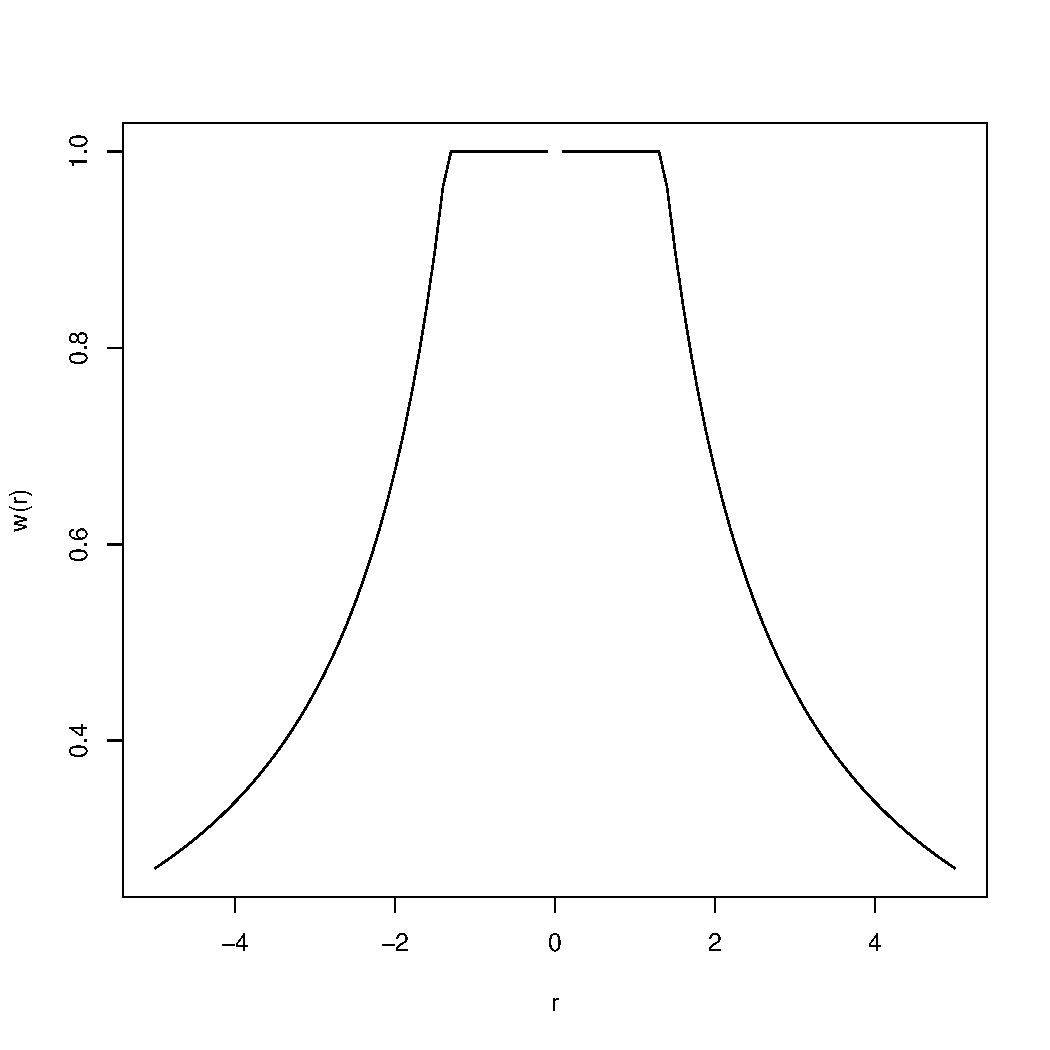
\includegraphics[width =4.5cm]{figures/Huberweights.pdf} 
\end{tabular}
\end{center}
\end{frame}

\begin{frame}
\frametitle{Choices for  $w({\bf x}_i)$}
Examples of weights $w({\bf x}_i)$:

\begin{itemize}
\item as a function of the diagonal elements of the hat
matrix $H = X (X^T X)^{-1} X^T$ (e.g.\ $w({\bf x}_i) = \sqrt{1-H_{ii}}$) 
\item based on the Mahalanobis distances of the design matrix (with the
center and the covariance matrix estimated robustly).
\end{itemize}

\bs
$\tilde{w}$ and $w$ can be used for diagnostic: they give information on how
each observation is handled.
\end{frame}


\begin{frame}
\frametitle{Properties of the robust GLM}
The distributional and robustness properties of the robust GLM estimator follow
from general results on M-estimation, with
$$M=\frac{1}{n} X^T B X \ \ \ \mbox{and} \ \ \ Q=\frac{1}{n} X^T A X  - a(\beta) a(\beta)^T,$$
where $B$ and $A$ are diagonal matrices containing elements
$$b_i = E[\psi_c(r_i) \frac{\partial}{\partial \mu_i} \log h(y_i |{\bf x}_i,
\mu_i)] \frac{1}{v^{1/2}(\mu_i)}  w({\bf x}_i) (\frac{\partial \mu_i}{\partial
\eta_i})^2,$$
and
$$a_i= E[\psi_c(r_i)^2] w^2({\bf x}_i)
\frac{1}{v(\mu_i)} ( \frac{\partial \mu_i}{\partial \eta_i})^2.$$

The influence function is bounded with respect to $y$ for a bounded choice of
$\psi$, and the effect of outliers in the design is controlled with
appropriate weights $w({\bf x})$.
\end{frame}


\begin{frame}
\frametitle{Variable selection}
The robust estimating equations of page~\pageref{EEw.page} can be seen as the
derivatives with respect to  $\beta$ of the {\color{blue}robust
quasi-likelihood} function $\sum_{i=1}^n Q_M(y_i, \mu_i)$, where
\begin{equation*}
\label{QM.explicit}
Q_M(y_i, \mu_i) = \int_{\tilde{s}}^{\mu_i} \phi(y_i, t) w({\bf x}_i)
dt - \frac{1}{n} \sum_{j=1}^n \int_{\tilde{t}}^{\mu_j} E \big[ \phi(y_j,t) w({\bf
x}_j) \big] dt,
\end{equation*}
where $\phi(y_i,t) = \psi\big((y_i-t)/v^{1/2}(t)\big)/v^{1/2}(t)$, $\tilde{s}$
and $\tilde{t}$ such that $\phi(y_i, \tilde{s}) = 0$, $
E[\phi(y_i,\tilde{t})] = 0$.

\bs
The above integrals are usually computed numerically.

\bs
Compare with the classical quasi-likelihood function on page~\pageref{QL.page}.
\end{frame}

\begin{frame}
\frametitle{}
To compare a model ${\mathcal M}_{p+1}$ with $(p+1)$ variables to a nested
model ${\mathcal M}_{p+1-q}$ with only $(p+1-q)$ variables,
a test statistic can be constructed based on twice the {\color{blue}difference
of quasi-likelihood} functions
\begin{equation*}
\label{quasi.dev}
\Lambda_{QM} = 2 \Big[ \sum_{i=1}^n Q_M(y_i, \hat{\mu}^{p+1}_i) - \sum_{i=1}^n
Q_M(y_i, \hat{\mu}^{p+1-q}_i) \Big].
\end{equation*}

\bs
Note that $\Lambda_{QM}$ is independent of $\tilde{s}$ and $\tilde{t}$.
\end{frame}

\begin{frame}
\frametitle{}
Under the null hypothesis that
$$H_0: \beta = (\cdot, \ldots, \cdot,0_{p+2-q},\ldots,0_{p+q})$$
and under quite general conditions, $\Lambda_{QM}$ is
asymptotically distributed as
$$\sum_{i=1}^q \lambda_i N_i^2,$$
where $N_1, \ldots,N_q \sim {\mathcal N}(0,1)$ and $\lambda_1, \ldots,
\lambda_q$ are the $q$ positive eigenvalues of the
matrix $Q(\psi,F_{\beta}) \big(M^{-1}(\psi,F_{\beta}) - \tilde{M}^{+}(\psi,
F_{\beta}) \big)$.

\bs
It can be proven that the asymptotic level and power under small deviations from
the model are stable as long as an estimator of $\beta$ with bounded influence
function is used.
\end{frame}

\subsection{Hospital costs dataset}
\begin{frame}
\frametitle{Example: Hospital costs of stay}

The Gamma distribution involves a second parameter $\nu$ that has also to be
estimated robustly. In fact this parameter is such
$$Var((Y_i - \mu_i)/v^{1/2}(\mu_i)) =1 / \nu,$$
 and therefore any robust estimator of the variance of $(Y_i -
\mu_i)/v^{1/2}(\mu_i)$ can be used, for example a simple M-estimator (Huber's
Proposal~2), which solves
\begin{equation*}
\label{nu.eq}
\sum_{i=1}^n \Big[ \psi_c\Big(\frac{y_i-\mu_i}{v^{1/2}(\mu_i)/\sqrt{\nu}} \Big)^2 -
E\Big(\psi_c\big(\frac{y_i-\mu_i}{v^{1/2}(\mu_i)/\sqrt{\nu}}\big)^2\Big) \Big]= 0,
\end{equation*}

\bs
The asymptotic results on $\beta$ still hold (for $\sqrt{n}$-consistent
estimator for $\nu$).
\end{frame}


\begin{frame}[fragile]
\frametitle{}

{\tiny
\begin{lstlisting}
Call:  glmrob(formula = CouTot ~ log(LOS) + Typadm + Typass + age +     
Sexe + dest, family = Gamma(link = log), data = MYdata) 

Coefficients:
              Estimate Std. Error z value Pr(>|z|)    
(Intercept)  7.2541684  0.1038707  69.838  < 2e-16 ***
log(LOS)     0.8391397  0.0197817  42.420  < 2e-16 ***
Typadm       0.2232685  0.0353717   6.312 2.75e-10 ***
Typass       0.0027594  0.0559621   0.049   0.9607    
age         -0.0010104  0.0009091  -1.111   0.2664    
Sexe         0.0711542  0.0353567   2.012   0.0442 *  
dest        -0.1243614  0.0490022  -2.538   0.0112 *  
---
Signif. codes:  0 ‘***’ 0.001 ‘**’ 0.01 ‘*’ 0.05 ‘.’ 0.1 ‘ ’ 1
Robustness weights w.r * w.x: 
 82 weights are ~= 1. The remaining 18 ones are summarized as
   Min. 1st Qu.  Median    Mean 3rd Qu.    Max. 
 0.2048  0.4902  0.6399  0.6208  0.7696  0.9925 

Number of observations: 100 
Fitted by method ‘Mqle’  (in 4 iterations)

(Dispersion parameter for Gamma family taken to be 0.02349196)

No deviance values available 
\end{lstlisting}
}
\end{frame}

\begin{frame}
\frametitle{}
  \begin{center}
  \begin{tabular}{|c|rr|rr|}
  \hline
  & \multicolumn{2}{c|}{Classical}  &   \multicolumn{2}{c|}{Robust}\\
   \hline
  variable  & coeff. & st.\ err. &  coeff. & st.\ err. \\
  \hline
  Intercept & 7.2338 & 0.1469 & 7.2523 & 0.1049 \\
  log(LOS) &  0.8222 & 0.0280 & 0.8391 & 0.0200 \\
  ADM & 0.2136 & 0.0500 & 0.2221 & 0.0357\\
  INS & 0.0933 & 0.0791 & 0.0093 & 0.0565\\
  AGE & -0.0005 & 0.0013 & -0.0010 & 0.0009\\
  SEX & 0.0951 & 0.0500 & 0.0727 & 0.0357\\
  DEST & -0.1043 & 0.0693 & -0.1230 & 0.0495 \\
  \hline
   & \multicolumn{2}{c|}{scale: 0.0496}  & \multicolumn{2}{c|}{scale: 0.0243}
  \\
  \hline
  \end{tabular}
  \end{center}
  
Similar coefficients, but larger standard errors.

\bs
Weights less or equal than $0.5$: $\tilde{w}_{14} = 0.23$,
$\tilde{w}_{21} = 0.50$, $\tilde{w}_{28} = 0.24$, $\tilde{w}_{44} = 0.42$ and
$\tilde{w}_{63} = 0.32$.

\end{frame}


\begin{frame}
\frametitle{Sensitivity analysis for variable selection}

\vspace*{-3cm}
\begin{center}
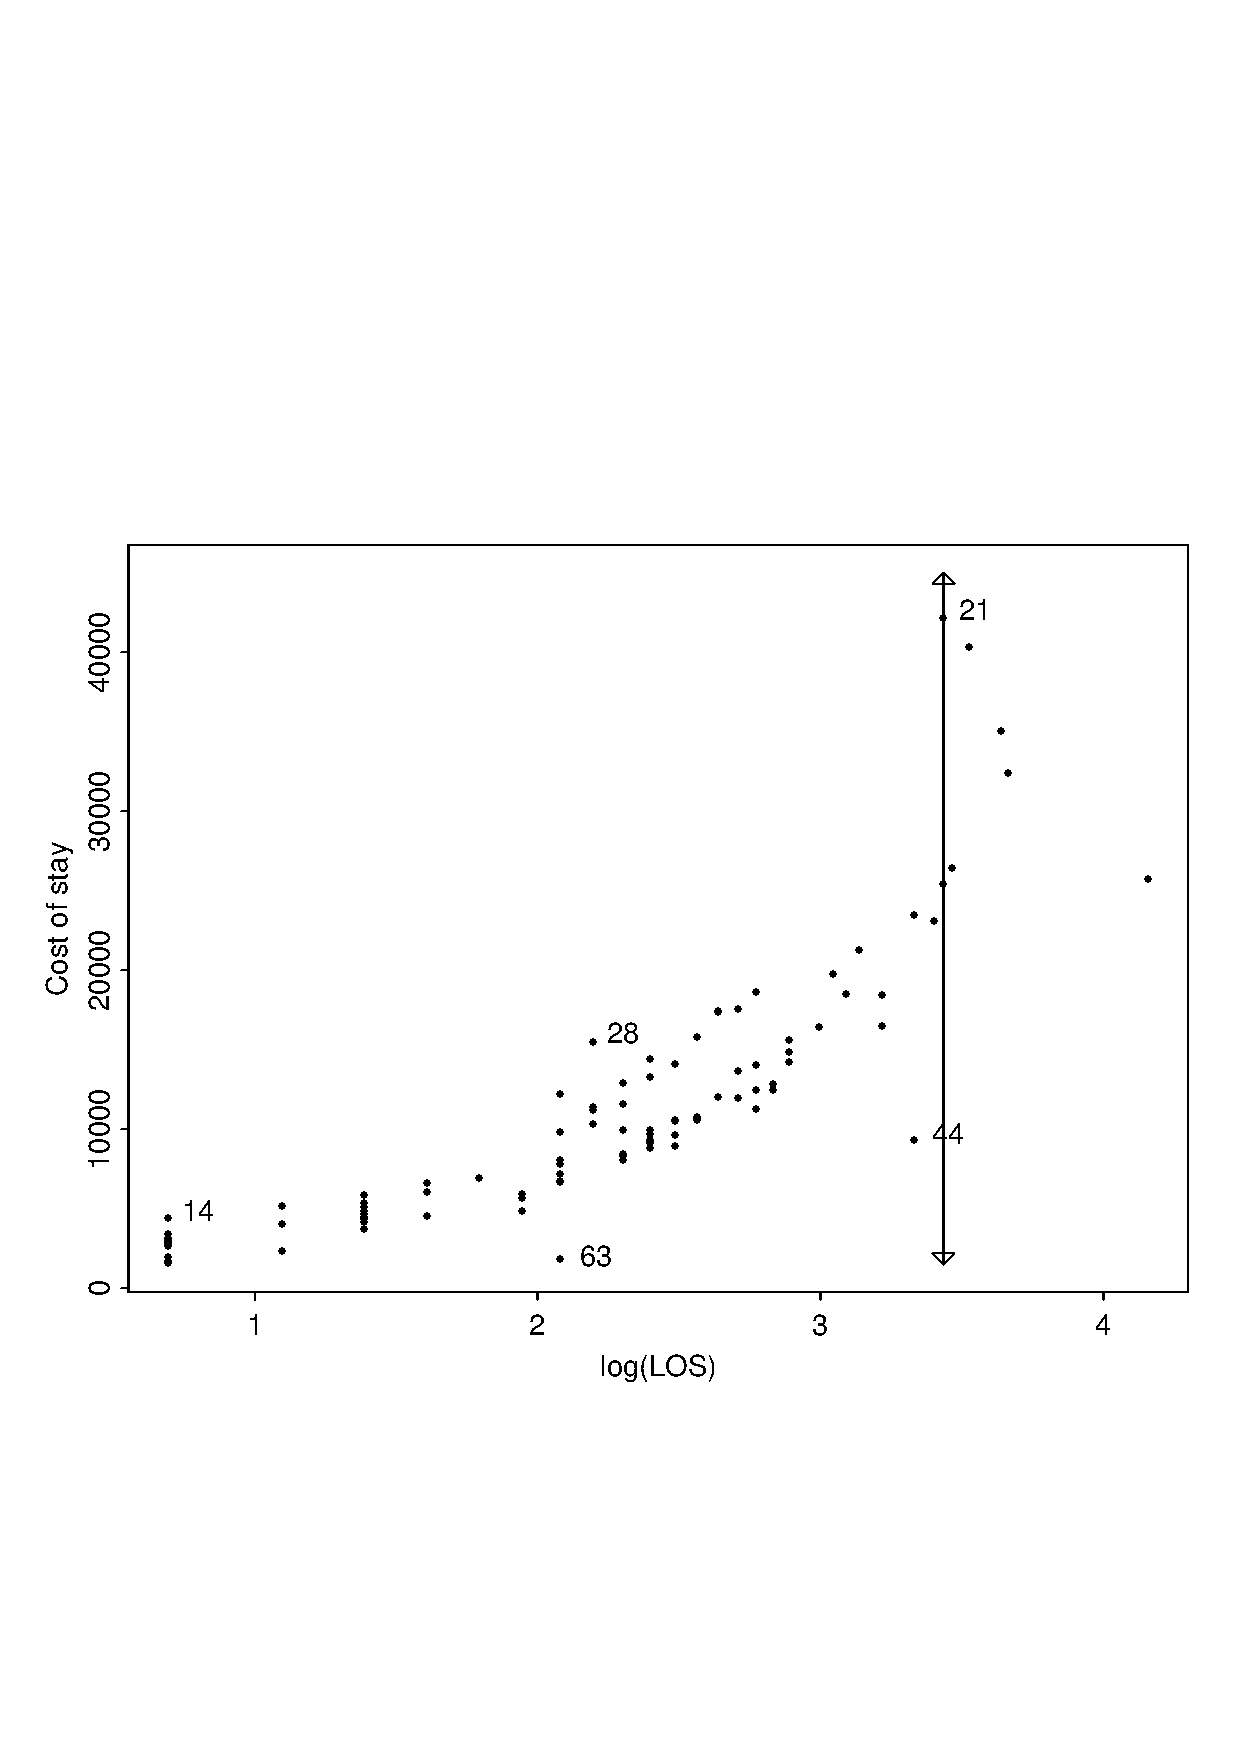
\includegraphics[width = 7.5cm]{figures/logLOScost.pdf}  
\end{center}
\end{frame}

\begin{frame}
\frametitle{p-values for the test of $H_0: \beta_{SEX}=0$.}
\begin{center}
\begin{tabular}{cc}
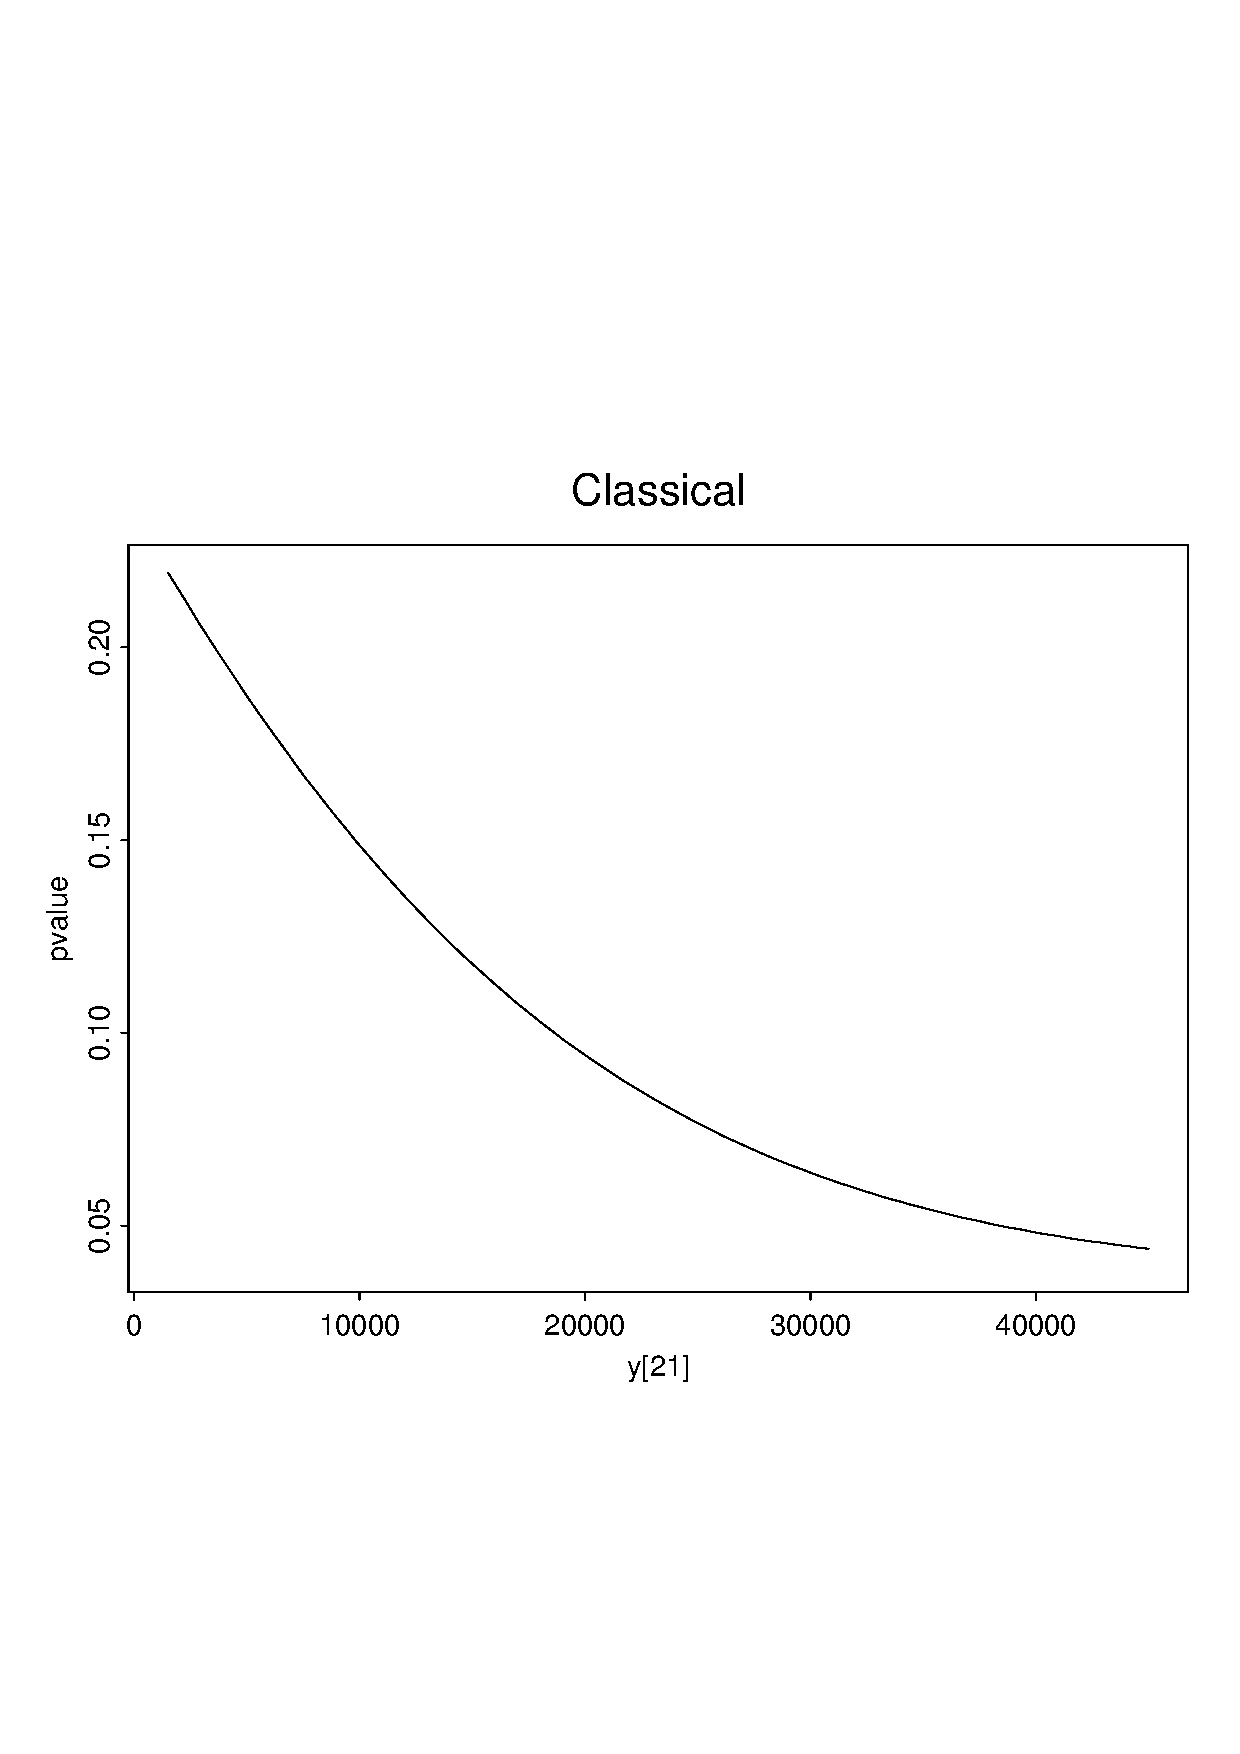
\includegraphics[width = 5cm]{figures/pvalueclass.pdf}  & 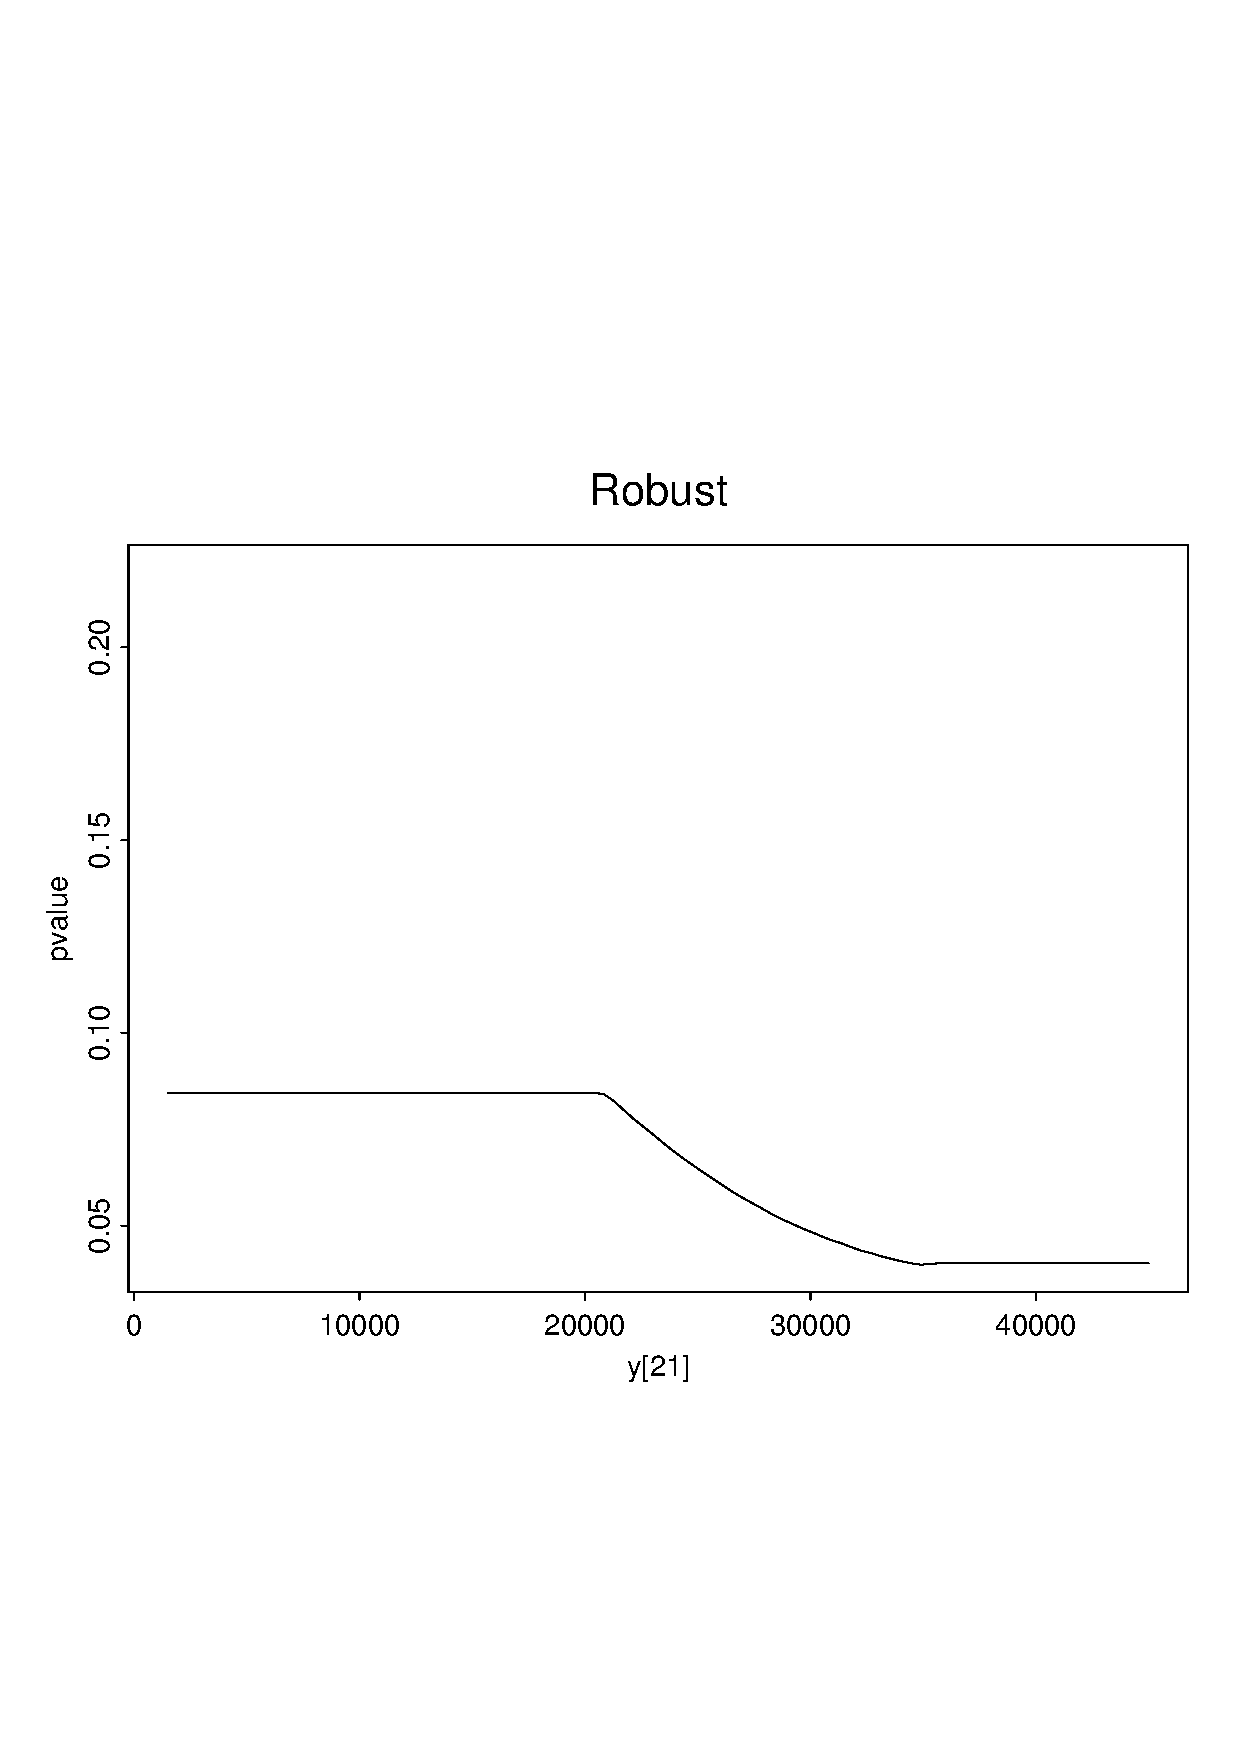
\includegraphics[width =5cm]{figures/pvaluerob.pdf} 
\end{tabular}
\end{center}
\end{frame}

\section{Robust GEE}
\begin{frame}
\frametitle{Robust GEE}

A {\color{blue}robust version of GEE} can be defined \cite{Cant:2004}:
$$\sum_{i=1}^n D_i^T \Gamma_i^T V_i^{-1} (\psi_i - c_i) =0,$$
where $D_i = \partial \mu_i / \partial \beta$, $V_i =
 \phi A_i^{1/2} R_i(\alpha) A_i^{1/2}$, with  $R_i(\alpha)$
the ``working'' correlation matrix.
Moreover, $\psi_i = W_i \cdot (Y_i - \mu_i)$, where $W_i = W_i(X_i, y_i, \mu_i)$
is a diagonal, and $c_i = E(\psi_i)$. Finally, $\Gamma_i = E(\tilde{\psi}_i -
\tilde{c}_i)$ with $\tilde{\psi}_i = \partial \psi_i / \partial \mu_i$ and $
\tilde{c}_i = \partial {c}_i / \partial \mu_i$.

\bs
The classical GEE equations are obtained with $W_i$ equal to the identity
matrix.

\bs
Estimation of $\phi$ and $\alpha$ has also to be made robust.

\end{frame}

\section{Robust hurdle model}
\begin{frame}
\frametitle{Robust hurdle model}

A {\color{blue}robust hurdle} model can be defined by building on each of its
two parts.

\bs
A robust binary regression is used to separate the zero from the positive
values. 

\bs
The robust GLM for truncated Poisson is also available \cite{Cant:Zedi:2011}. It
uses the GLM framework of the truncated Poisson (see page
\pageref{truncpoisdef}) and defines  the estimator wiht the estimating equations
of page~\pageref{EE.eq}. 
\end{frame}

\section{Generalized additive models (GAM)}
\label{GAM.section}

\subsection{Univariate smoothing}
\begin{frame}
\frametitle{Generalized additive models (GAM)}

Consider the same kind of models as for GLM
(exponential family distributions for continuous and discrete
variables, link functions, etc), but replace the linear part of GLM
with nonparametric functions:

$$g(\mu_i) = \alpha + f_1(x_{i1}) + \ldots + f_p(x_{ip}).$$

This new model is particularly useful when no functional form is
known a priori. It is also a way to check whether the linear (or other
parametric) assumption is sensible.

\begin{center}
{\color{blue}Let the data show us the appropriate functional form.}
\end{center}
from \citeN{Hast:Tibs:1990}, p.~1.

\end{frame}

\begin{frame}
\frametitle{Univariate smoothing}

Data: $(x_i,y_i)$ for individuals $i=1,\ldots,n$.

\bs
We start with the simple univariate model
$$Y_i = f(x_i) + \epsilon_i,$$

with the assumption that the $\epsilon_i$ are independently drawn from $N(0, \sigma^2)$.

\bs
It is the univariate nonparametric analogue to
$$Y_i = \alpha + \beta x_i + \epsilon_i.$$
\end{frame}


\begin{frame}
\frametitle{Ethanol example}

Engine exhaust for 88 burnings of ethanol in a single-cylinder automobile test
engine. Outcome: concentration of nitric oxides (\texttt{NOx}). Explanatory
variable: equivalence ratio, that is a measure of the richness of the
air/ethanol mix (\texttt{E}).

\begin{center}
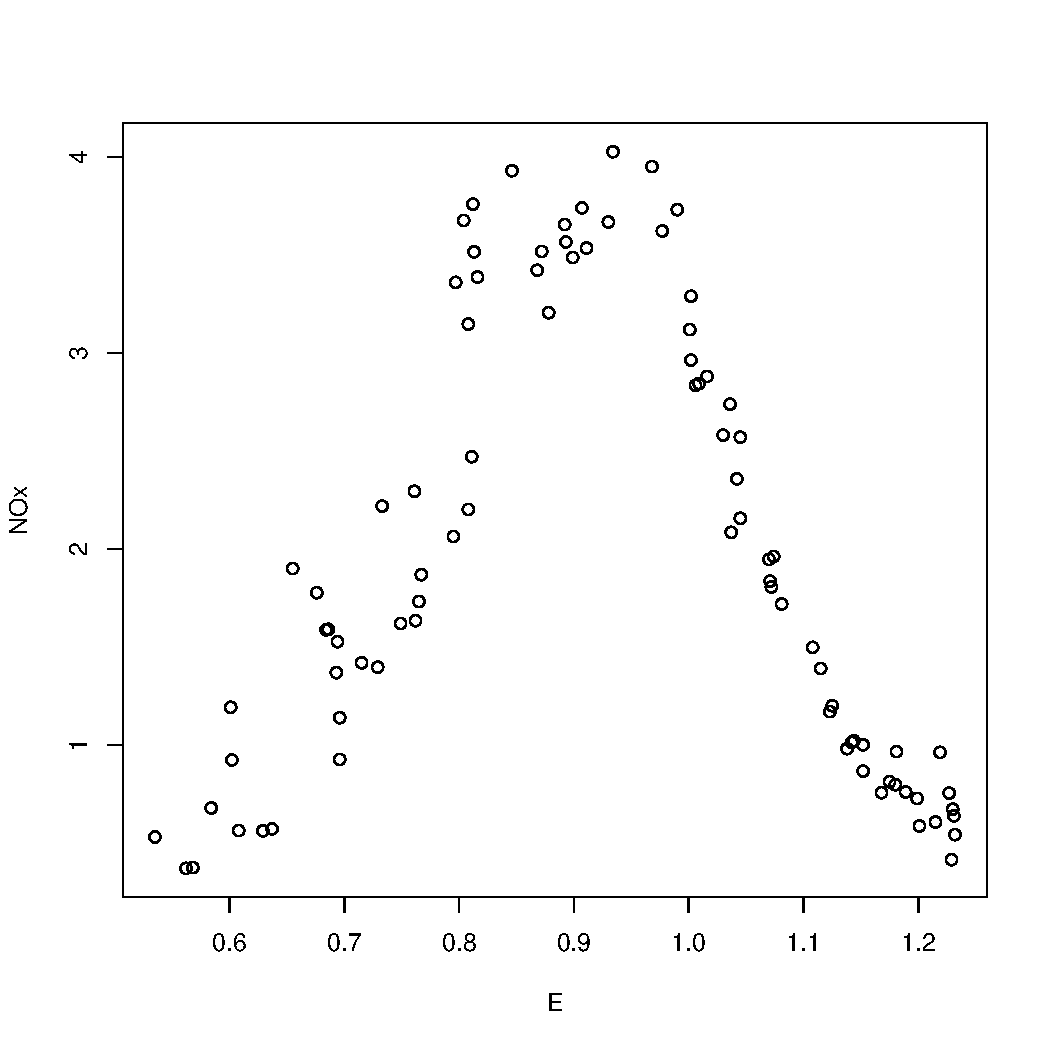
\includegraphics[width = 5cm]{figures/ethanol.pdf}  
\end{center}

\end{frame}

\begin{frame}
\frametitle{Nonparametric vs quadratic fit}
\begin{center}
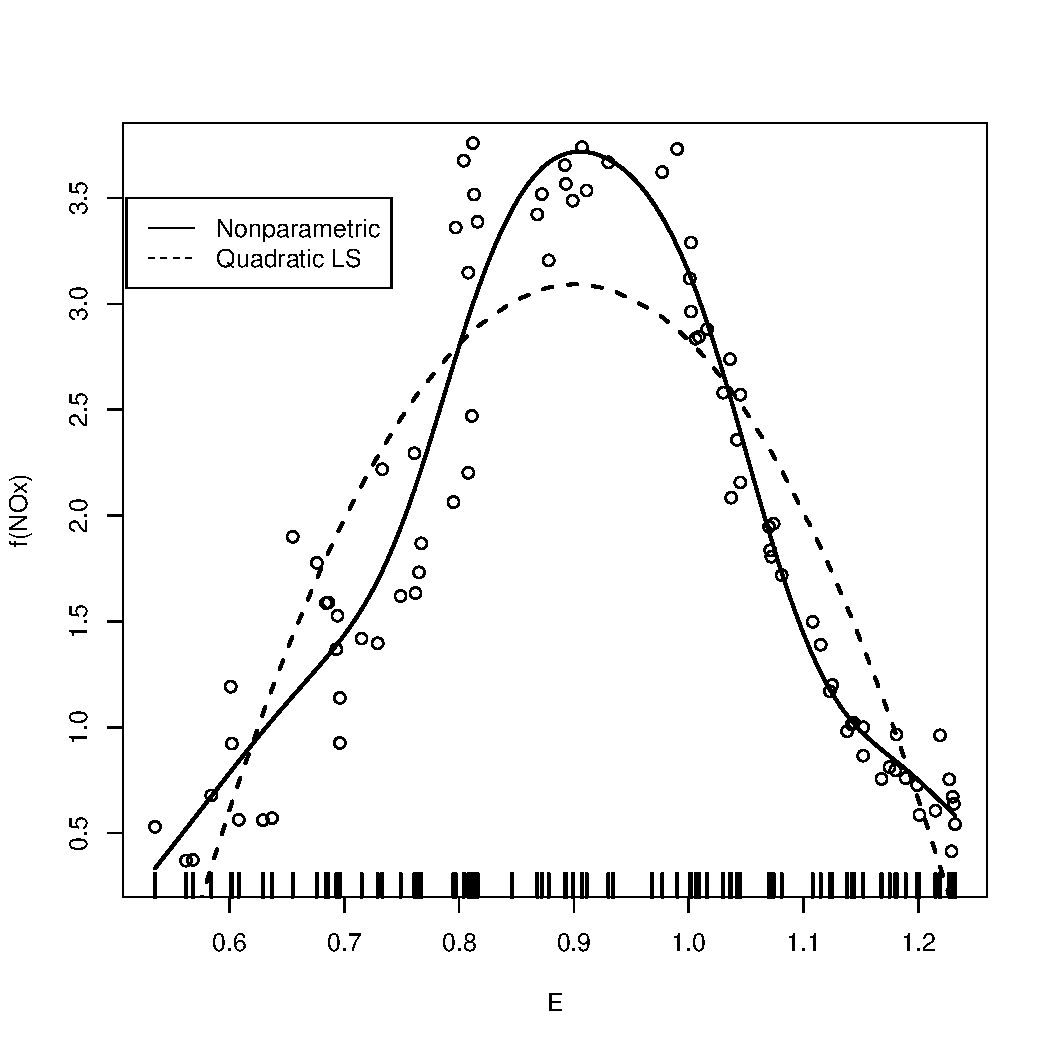
\includegraphics[width = 7cm]{figures/ethanolFit.pdf}  
\end{center}
\end{frame}

\begin{frame}
\frametitle{Basis functions}

How to represent $f(x)$? With an approximation with known functions:
$$f(x) = \sum_{k=1}^K  b_k(x) \beta_k,$$ where the $b_k(x)$ are basis functions.
 The model is therefore 
 $$Y_i = \sum_{k=1}^K  b_k(x_i) \beta_k + \epsilon_i, $$
 for $i=1,\ldots,n$.
 \end{frame}

\begin{frame}
\frametitle{Model fitting}
For $Y  = (Y_1, \ldots,Y_n)^T$, $\beta = (\beta_1, \ldots, \beta_K)^T$ and
$\epsilon = (\epsilon_1,\ldots,\epsilon_n)$, the model can be  equivalently expressed as
$$Y = X \beta + \epsilon,$$
with
$$X = \left( 
\begin{array}{cccc}
b_1(x_1) & b_2(x_1)  & \ldots  & b_K(x_1) \\
\vdots & \vdots & \vdots & \vdots \\
b_1(x_n) & b_2(x_n)  & \ldots  & b_K(x_n) \\
\end{array} \right).$$

\bs
It can be fitted by least squares:
 $$\hat{\beta} = \mbox{argmin}_{\beta}  ||y - X \beta ||^2.$$
 
\end{frame}

\begin{frame}
\frametitle{Polynomial basis}

If $f$ is believed to be a 4th order polynomial, a possible basis is
$$b_1(x) = 1, b_2(x) = x, b_3(x) = x^2, b_4(x) = x^3, b_5(x) = x^4,$$ 
so that 
$$f(x)  = \beta_1 + x \beta_2  + x^2 \beta_3 + x^3 \beta_4 + x^5 \beta_5$$
and the model
$$y_i = \beta_1 + x_i \beta_2  + x_i^2 \beta_3 + x_i^3 \beta_4 + x_i^5 \beta_5 + \epsilon_i,$$
\end{frame}

\begin{frame}
\frametitle{The piecewise linear (or tent) basis - formula}

Given knots $x_j^*$, for $j=1,\ldots,k,$ with $x_j^* > x_{j-1}^*$, we have  for $j=2, \ldots, k-1$: 

$$b_j(x) = \left\{ 
\begin{array}{cc}
(x - x_{j-1}^*)/(x_j^* - x_{j-1}^*) & x_{j-1}^* < x < x_j^* \\
 (x_{j+1}^* - x)/(x_{j+1}^* - x_{j}^*) & x_{1}^* < x < x_{j+1}^* \\
 0 & \mbox{otherwise}
\end{array} \right.$$

$$b_1(x) = \left\{ 
\begin{array}{cc}
 (x_{2}^* - x)/(x_{2}^* - x_{1}^*) &  x < x_{2}^* \\
 0 & \mbox{otherwise}
\end{array} \right.$$

$$ b_k(x) = \left\{ 
\begin{array}{cc}
(x - x_{k-1}^*)/(x_k^* - x_{k-1}^*) &  x > x_{k-1}^* \\
 0 & \mbox{otherwise}
\end{array} \right.$$
\end{frame}

\begin{frame}
\frametitle{The piecewise linear (or tent) basis - graphical representation }

\begin{center}
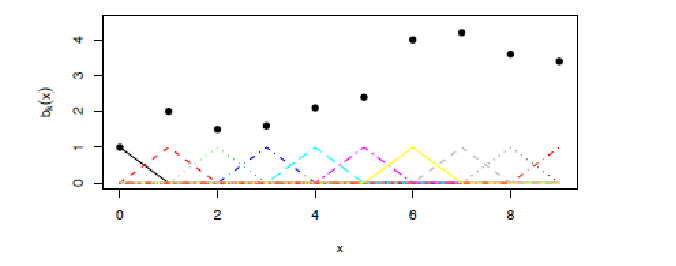
\includegraphics[width = 12cm]{figures/TentBasis.pdf}  
\footnote{Figure from S. Wood slides at the \textit{Ecole doctorale d'hiver CUSO}, 2014, Les Diablerets}
\end{center}
\end{frame}


\begin{frame}
\frametitle{Approximation of $f$ }

Data $(x_k^* , y_k^*)$ are interpolated by just setting $\beta_k = y_k^*$. The function $f$ is represented by multiplying each tent function by its coefficient $\beta_k$ and summing the result.

\begin{center}
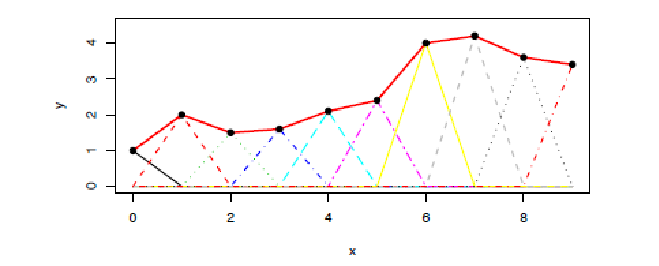
\includegraphics[width = 9cm]{figures/TentApprox.pdf}  
\footnote{Figure from S. Wood slides at the \textit{Ecole doctorale d'hiver CUSO}, 2014, Les Diablerets}
\end{center}
\end{frame}

\begin{frame}
\frametitle{}
In practice: choose some $x_k^*$ values spread through the range of the observed $x_i$'s. 

\vspace*{-0.5cm}
\begin{center}
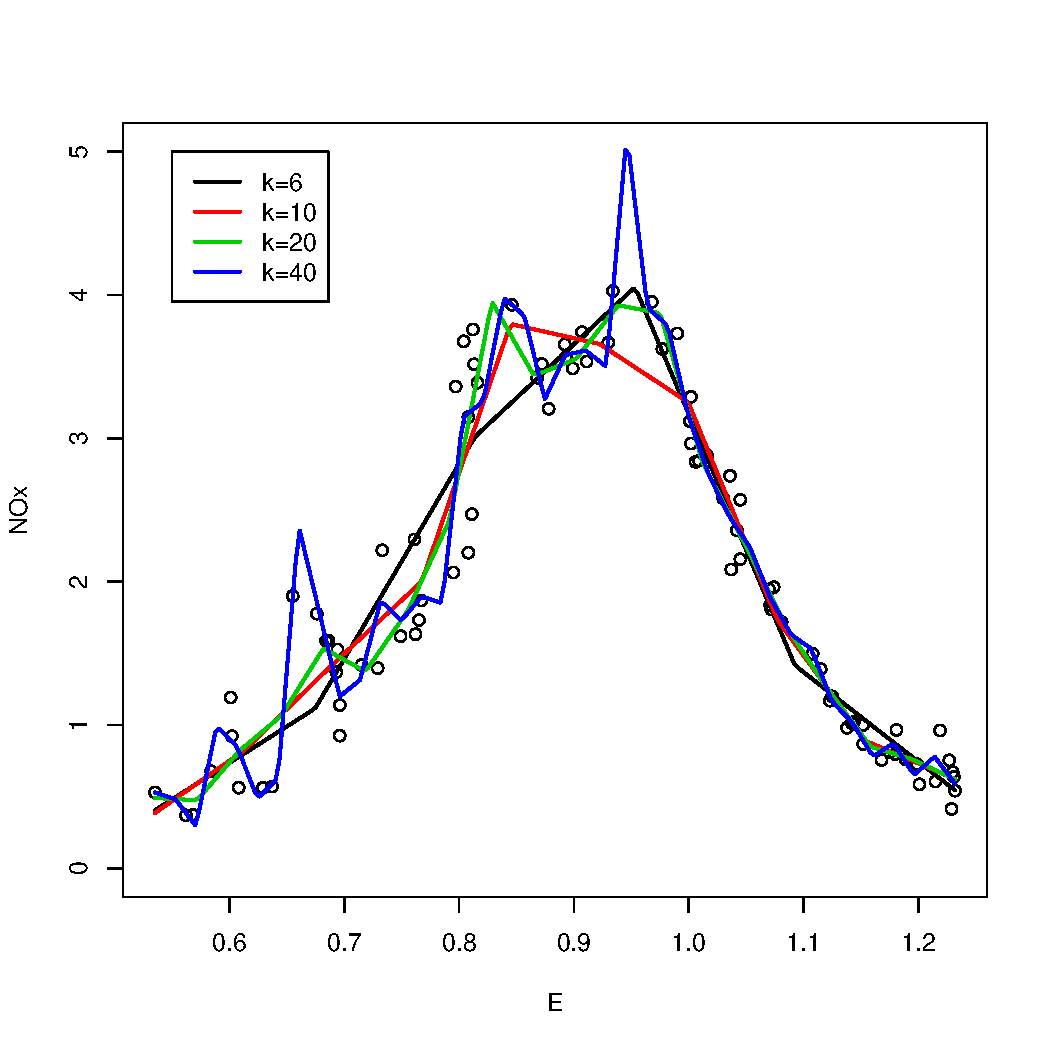
\includegraphics[width = 7.5cm]{figures/EthanolK.pdf}  
\end{center}

\end{frame}


\begin{frame}
\frametitle{Other bases: splines}
The polynomial and the tent bases are easy to understand, but improvement is
possible. In particular, spline bases reduce function approximation error for a
given dimension of the smoothing basis.

\bs  
A cubic smoothing spline solves (with respect to $f$)
$$\sum_{i=1}^n \left(y_i - f(x_i) \right)^2 + \lambda \int (f^{\prime
\prime}(x))^2 dx.$$

Cubic splines arise naturally from the specification of the smoothing objective
function above (defined in a basis independent way).


\end{frame}

\begin{frame}
\frametitle{}
The drawback of smoothing splines is that they have $n$ free parameters. To
retain their good properties, but improve on computational efficiency, penalized
regression splines are used instead.

\bs
It implies constructing a spline basis for a much
smaller data set and then using
that basis (plus penalties) to model the original dataset. The covariates values
in the smaller dataset should be chosen to nicely cover the range of the
covariates in the original dataset.

\end{frame}



\begin{frame}
\frametitle{Informal basis dimension check}

Perform a check to see whether $k$ is not restrictively low.

\begin{enumerate}
\item Look at partial residuals against term estimates, looking for systematic departures
\item Use a residual randomization test to test for residuals pattern.\\
Idea: estimate the scale parameter $\sigma^2$ by differencing
residuals. Differencing residuals that are neighboring according to  $x_i$ should
give an estimate of $\sigma^2$ that is indistinguishable from a differencing
estimate obtained with any random ordering of residuals, under the null
hypothesis that there is no residual pattern. 
\end{enumerate}
\end{frame}


\begin{frame}
\frametitle{Ethanol example with regression splines}

\vspace*{-0.5cm}
\begin{center}
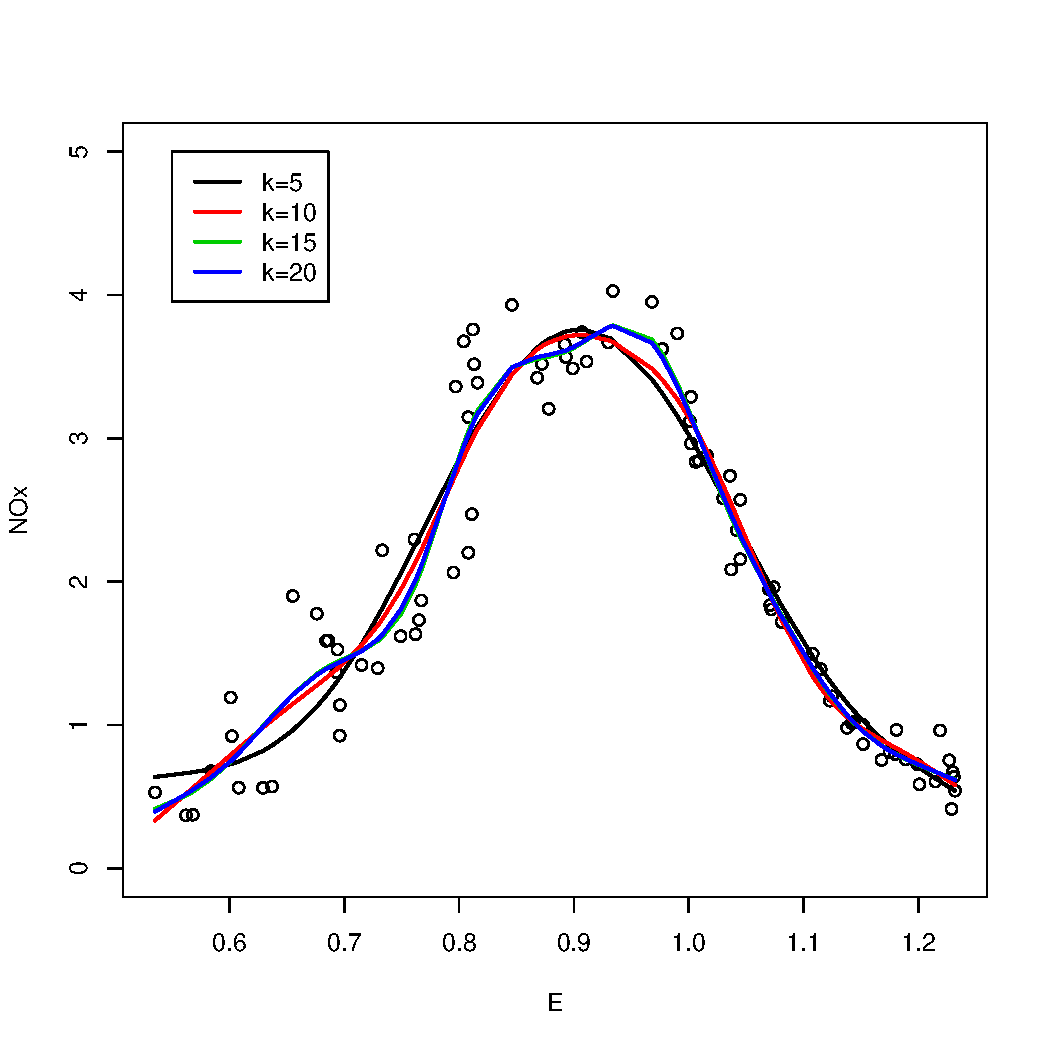
\includegraphics[width = 7.5cm]{figures/EthanolKsplines.pdf}  
\end{center}
\end{frame}

\begin{frame}
\frametitle{Partial residuals}

\vspace*{-0.5cm}
\begin{center}
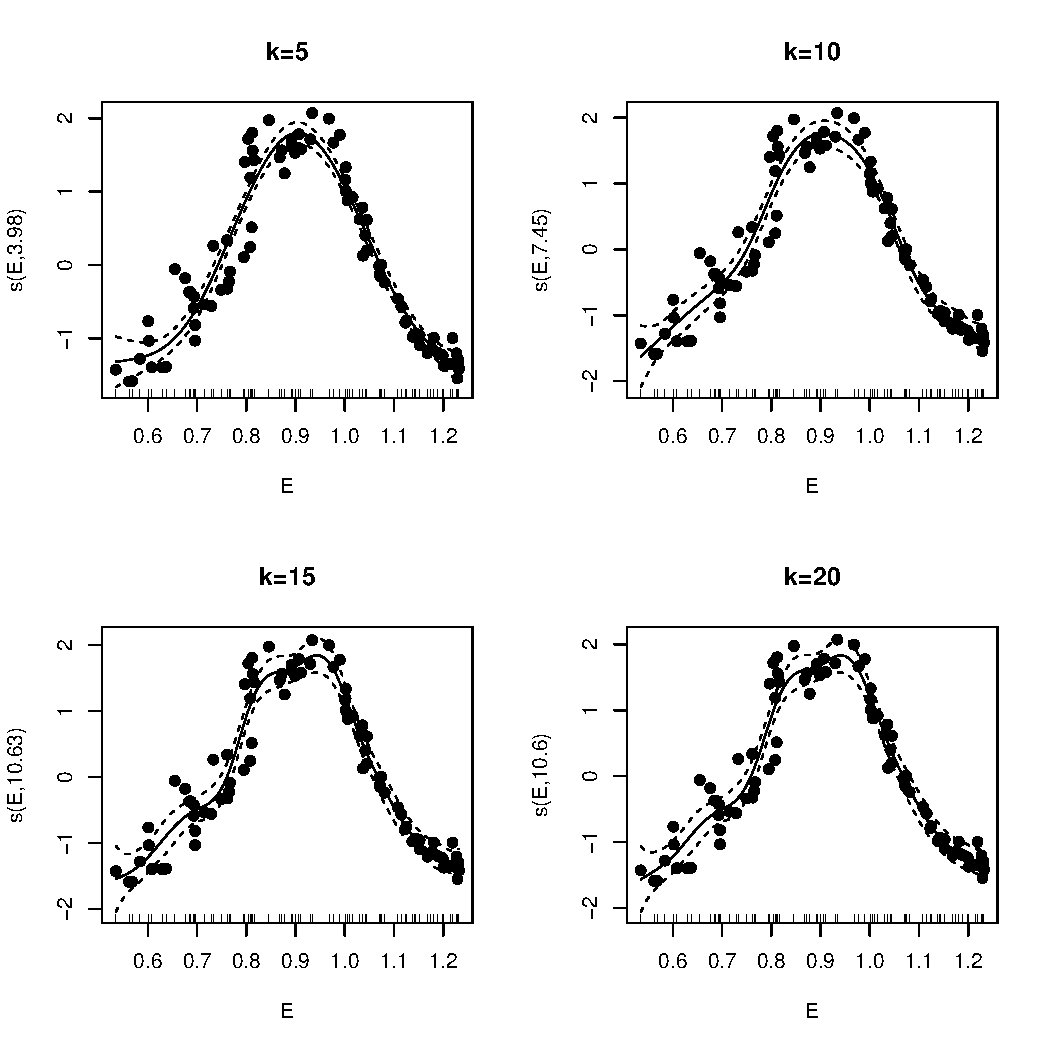
\includegraphics[width = 7.5cm]{figures/EthanolKresid.pdf}  
\end{center}
\end{frame}

\begin{frame}[fragile]
\frametitle{}

{\scriptsize
\begin{lstlisting}
ethanol1 <- gam(NOx~s(E,k=5),data=ethanol)

> gam.check(ethanol1)

Method: GCV   Optimizer: magic
Smoothing parameter selection converged after 10 iterations.
The RMS GCV score gradient at convergence was 3.154738e-06 .
The Hessian was positive definite.
Model rank =  5 / 5 

Basis dimension (k) checking results. Low p-value (k-index<1) may
indicate that k is too low, especially if edf is close to k'.

                k'   edf k-index p-value
s(ethanol$E) 4.000 3.982   0.682       0
\end{lstlisting}
}
\end{frame}


\begin{frame}[fragile]
\frametitle{}

{\scriptsize
\begin{lstlisting}
ethanol2 <- gam(NOx~s(E,k=10),data=ethanol)

> gam.check(ethanol2)

Method: GCV   Optimizer: magic
Smoothing parameter selection converged after 8 iterations.
The RMS GCV score gradient at convergence was 2.421344e-06 .
The Hessian was positive definite.
Model rank =  10 / 10 

Basis dimension (k) checking results. Low p-value (k-index<1) may
indicate that k is too low, especially if edf is close to k'.

                k'   edf k-index p-value
s(ethanol$E) 9.000 7.452   0.766       0
\end{lstlisting}
}

\end{frame}

\begin{frame}[fragile]
\frametitle{}

{\scriptsize
\begin{lstlisting}
ethanol3 <- gam(NOx~s(E,k=15),data=ethanol)

> gam.check(ethanol3)

Method: GCV   Optimizer: magic
Smoothing parameter selection converged after 8 iterations.
The RMS GCV score gradient at convergence was 1.551372e-05 .
The Hessian was positive definite.
Model rank =  15 / 15 

Basis dimension (k) checking results. Low p-value (k-index<1) may
indicate that k is too low, especially if edf is close to k'.

                 k'    edf k-index p-value
s(ethanol$E) 14.000 10.633   0.884    0.11

\end{lstlisting}
}
\end{frame}


\begin{frame}[fragile]
\frametitle{}

{\scriptsize
\begin{lstlisting}
ethanol4 <- gam(NOx~s(E,k=20),data=ethanol)

> gam.check(ethanol4)

Method: GCV   Optimizer: magic
Smoothing parameter selection converged after 6 iterations.
The RMS GCV score gradient at convergence was 1.246923e-06 .
The Hessian was positive definite.
Model rank =  20 / 20 

Basis dimension (k) checking results. Low p-value (k-index<1) may
indicate that k is too low, especially if edf is close to k'.

                 k'    edf k-index p-value
s(ethanol$E) 19.000 10.603   0.872    0.09
\end{lstlisting}
}
\end{frame}

\begin{frame}
\frametitle{More formal choice of $K$?}

\begin{itemize}
\item Models with different $K$ are not nested: rules out hypothesis testing.
\item Need to fit all possible $K$ value if wants to use e.g.\ AIC
\item Difficult to generalize to models with more than one function
\end{itemize}

\bs
In addition, where to put the knots?

\end{frame}


\begin{frame}
\frametitle{Smoothing}

Instead of selecting $K$, rather use \textit{smoothing}:

\begin{itemize}
\item Make $K$ `large enough' (negligible bias)
\item Use even spaced $x_k^*$
\item To avoid overfit, penalize the wiggliness of $f$, e.g.\ with 

$${\cal P} (f) = \sum_{j=2}^{k-1} \{f(x_{j-1}^*) - 2 f(x_j^*) + f(x_{j+1}^*) \}^2.$$
This penalty can be regarded as  a crude approximation of the second derivative of $f$.

\bs
When $f$ is wiggly the penalty is large, when $f$ is smooth the penalty is low. (The penalty is zero for a straight line).
\end{itemize}
\end{frame}

\begin{frame}
\frametitle{}
The model is fitted by maximisation of the penalized least squares criterion
 $$\hat{\beta} = \mbox{argmin}_{\beta} \{  ||y - X \beta ||^2 + \lambda {\cal P}(f) \}.$$

\bs
The \textit{smoothing parameter} $\lambda$ controls the trade-off between smoothness of the estimated $f$ and fidelity to the data.

\bs
 $\lambda \rightarrow \infty$ leads to a straight line estimate for $f$ while $\lambda=0$ results in an unpenalized piecewise linear regression estimate.
\end{frame}

\begin{frame}
\frametitle{Smoothing with the tent basis}
For the tent basis, it holds that $\beta_j = f(x_j^*)$ and therefore the penalty can be expressed as a quadratic form, because
$$ \left( 
\begin{array}{c}
\beta_1 - 2 \beta_2 + \beta_3 \\
\beta_2 - 2 \beta_3 + \beta_4 \\
\beta_3 - 2 \beta_4 + \beta_5 \\
\vdots
\end{array}
\right) = \left[
\begin{array}{ccccccc}
1 & -2 & 1 & 0 & . & . & . \\
0 & 1 & -2 & 1 & 0 & . & . \\
0 & 0 & 1 & -2 & 1 & 0 & . \\
\vdots & \vdots &\vdots &\vdots &\vdots &\vdots &\vdots \\
\end{array}
\right]  \left[
\begin{array}{c}
\beta_1 \\
\beta_2 \\
\beta_3 \\
\vdots
\end{array}
\right] = D \beta
$$
and therefore 
$$ {\mathcal P}(f) = \sum_{j=2}^{k-1} \{f(x_{j-1}^*) - 2 f(x_j^*) + f(x_{j+1}^*) \}^2 = \beta^T D^T D \beta = \beta^T S \beta$$
\end{frame}

\begin{frame}
\frametitle{Smoothing (general)}
We solve
 $$\hat{\beta} = \mbox{argmin}_{\beta} \{  ||y - X \beta ||^2 + \lambda  \beta^T S \beta \},$$
which has the explicit solution
 $$\hat{\beta} = (X^T X + \lambda S)^{-1} X^T y.$$
 
\bs
Therefore 
$$ \hat{y} = \hat{f}(x) = X \hat{\beta} = X (X^T X + \lambda S)^{-1} X^T y = A y,$$
where $A= X (X^T X + \lambda S)^{-1} X^T$ is the influence (hat) matrix. 

\label{linear.smoother}

\end{frame}

\begin{frame}
\frametitle{}
For computational stability, note that the problem is transformed in an augmented form as follow:
 $$\{  ||y - X \beta ||^2 + \lambda  \beta^T S \beta \} = \left|\left| \left[
 \begin{array}{c}
y \\
0
\end{array}
 \right] - \left[
 \begin{array}{c}
 X  \\
 \sqrt{\lambda} D
  \end{array}
 \right] \beta \ 
  \right|\right|^2,$$
which is a least squares problem.
\end{frame}


\begin{frame}
\frametitle{Natural basis}

For any model matrix $X$ and penalty matrix $S$ we can consider the
reparametrization that makes the penalty matrix diagonal.

\bs
Let $X= Q R$ (QR decomposition), and $R^{-T} S R^{-1} = U \Lambda U^{T}$ (SVD
decomposition).

\bs
Define $P = U^T R$ and reparametrize $\beta^{\prime} = P \beta$.

\bs 
In the new parametrization, the model matrix is $X^{\prime} = Q U$, which has
orthogonal columns ($X = X^{\prime}P$). The penalty matrix is now the diagonal
matrix $\Lambda$.
\end{frame}


\begin{frame}
\frametitle{Degrees of freedom}
Penalization restricts the freedom of coefficients to vary: $K$ coefficients have
$< K$ \textit{effective degrees of freedom} (edf).

\bs 
Consider a natural parametrization. 

\bs 
Without penalization: $ \tilde{\beta}^{\prime} =  ( X^{\prime} )^T  y$
 
With penalization: $\hat{\beta}^{\prime} = (I + \lambda \Lambda)^{-1}  ( X^{\prime} )^T
y$, therefore $\hat{\beta}_j ^\prime = 
\tilde{\beta}_j^\prime (1 +\lambda \Lambda_{jj})^{-1}$. So $(1 + \lambda \Lambda_{jj})^{-1}$ is the
shrinkage factor of the $j^{th}$ coefficient. It gives the EDF for
$\hat{\beta}_j$.

\bs
The total EDF is $\sum_{j} (1 + \lambda  \Lambda_{jj})^{-1} = Tr(F)$ with $F = (X^T X +
\lambda S)^{-1} X^T X$. 
\end{frame}


\begin{frame}
\frametitle{Smoothing bias}

Because $\hat{\beta} = (X^T X + \lambda S)^{-1} X^T y$, it holds that
\begin{eqnarray*}
E(\hat{\beta}) & = & (X^T X + \lambda S)^{-1} X^T E(y) \\
 & = & (X^T X + \lambda S)^{-1} X^T X \beta \\
& = & F \beta \neq \beta
\end{eqnarray*}

Smooths are biased due to the penalization.

\bs
This bias makes frequentist inference difficult.
\end{frame}

\begin{frame}
\frametitle{The Bayesian paradigm in a nutshell}

With the distribution $f(y \mid \beta) $ of $(y \mid \beta)$ 
and the {\color{blue}prior distribution} $\pi(\beta)$ on the parameter $\beta$,
construct a 
{\color{blue}posterior distribution}, that is the 
distribution of $\beta \mid y$, which is (thanks to Bayes theorem):
$$  \pi(\beta \mid y) = \frac{ f(y \mid \beta) \pi(\beta)}{f(y)} .$$


\bs
Inference is conducted on the basis of the posterior distribution.

\end{frame}

\begin{frame}
\frametitle{Illustration of the Bayesian paradigm}

\begin{center}
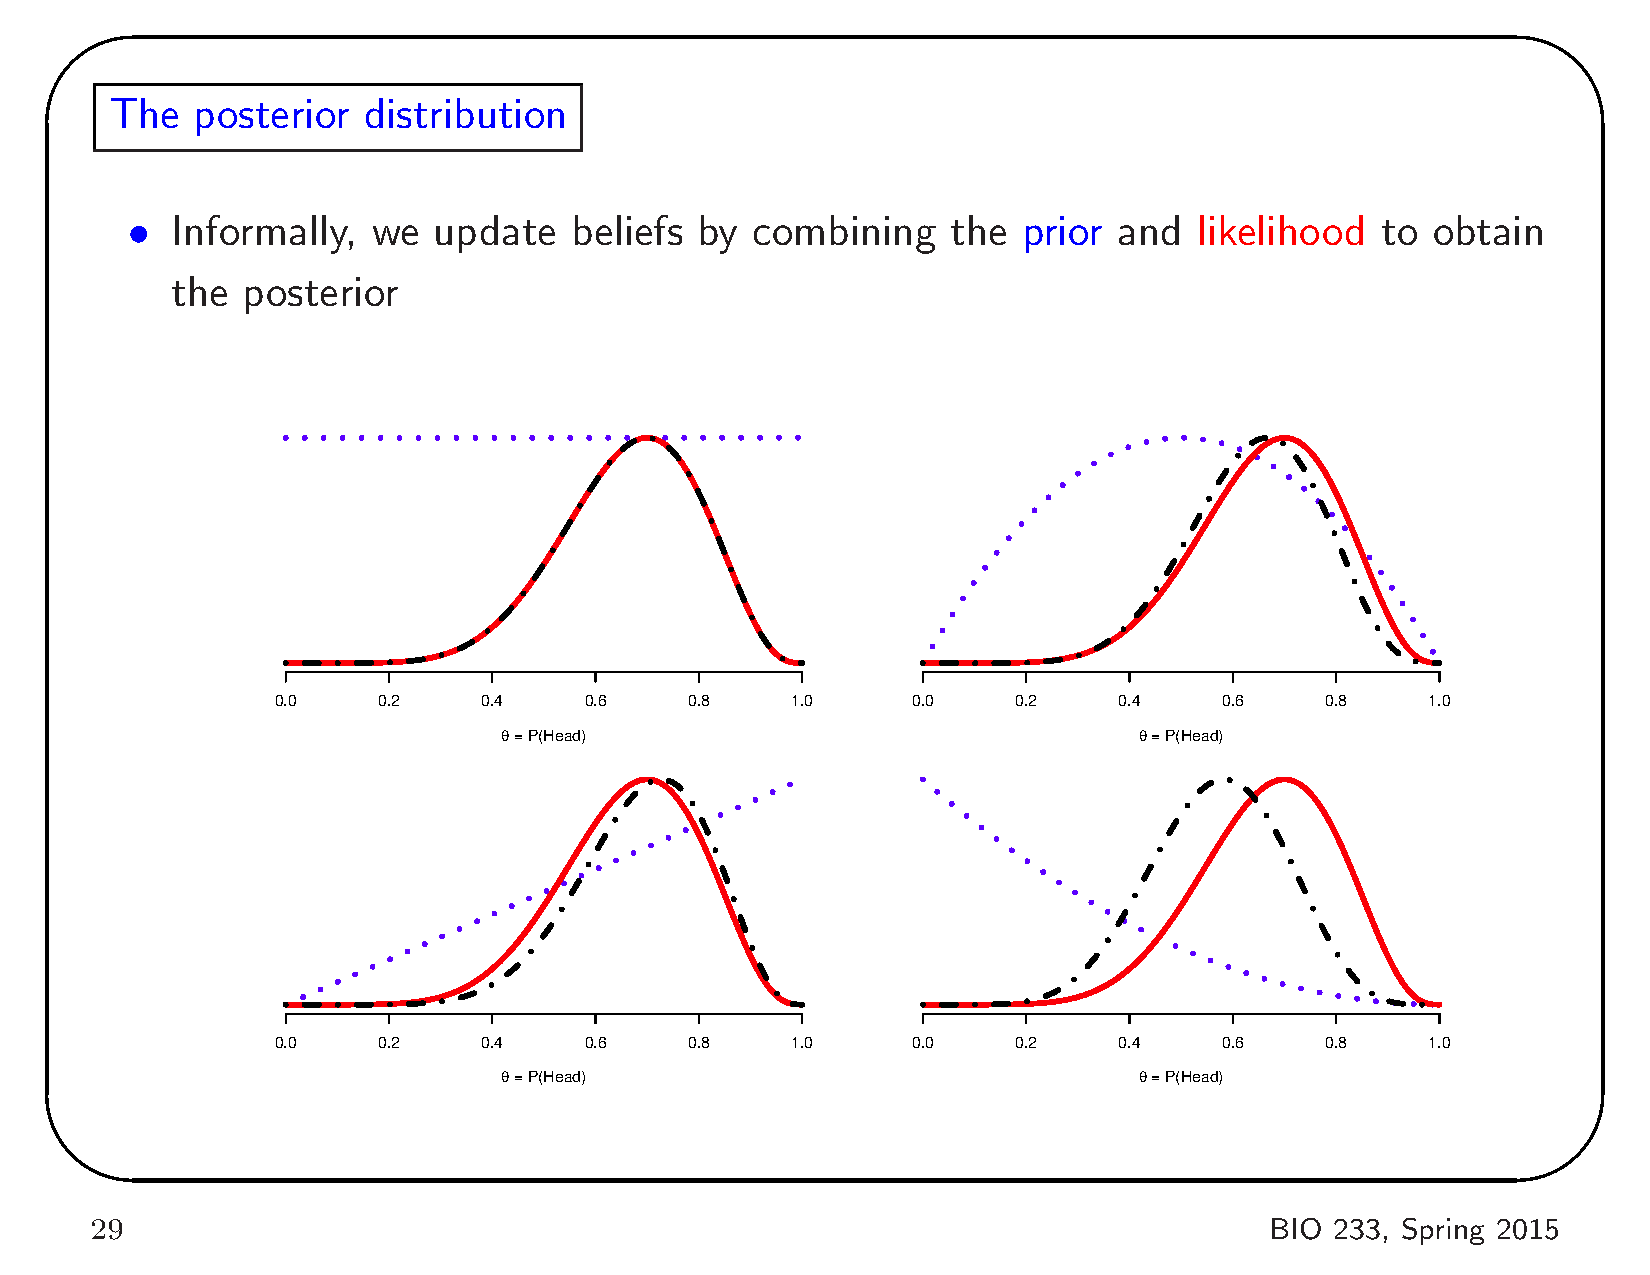
\includegraphics[width = 7.5cm]{figures/BayesParadigm.pdf}  
\end{center}

\vspace*{-1cm}
{\tiny From: 
\texttt{https://cdn1.sph.harvard.edu/wp-content/uploads/sites/565/2018/08/233Spr15\char`_Part1\char`_Bayes.pdf}
}
\end{frame}


\begin{frame}
\frametitle{Bayesian smoothing model}
The penalization can be seen as a prior put on wiggliness in a Bayesian
framework:

$$\mbox{wiggliness prior} \propto \exp\left( - \lambda \beta^T S \beta /(2
\sigma^2)\right)$$
equivalent to a prior $\beta \sim {\mathcal N}(0,S^{-} \sigma^2/\lambda)$, where
$S^{-} $ is a generalized inverse of $S$.

\bs
From the model we have $y\mid \beta \sim  {\mathcal N}(X \beta, \sigma^2 I)$,
therefore (Bayes rule) 
$$\beta \mid y \sim {\mathcal N}(\hat{\beta}, \sigma^2 (X^T X + \lambda
S)^{-1}).$$

\bs
Also: $\hat{\sigma} ^2 = ||y - X \hat{\beta}||^2/ (n - Tr(F))$.

\end{frame}

\begin{frame}
\frametitle{Ethanol example with different $\lambda$ (tent basis)}

\vspace*{-0.5cm}
\begin{center}
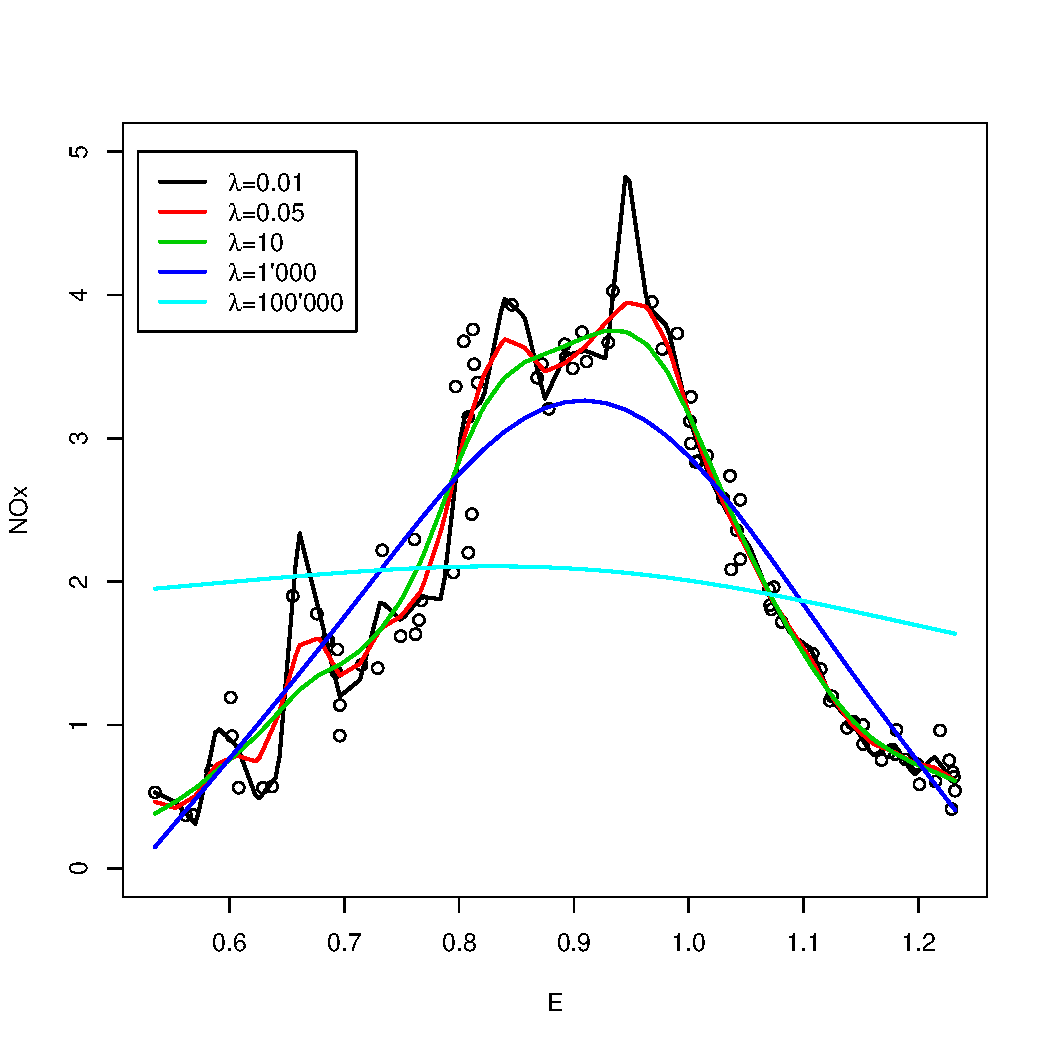
\includegraphics[width = 7.5cm]{figures/Ethanollambda.pdf}  
\end{center}
\end{frame}

\begin{frame}
\frametitle{Ethanol example with different $\lambda$ (spline basis)}

\vspace*{-0.5cm}
\begin{center}
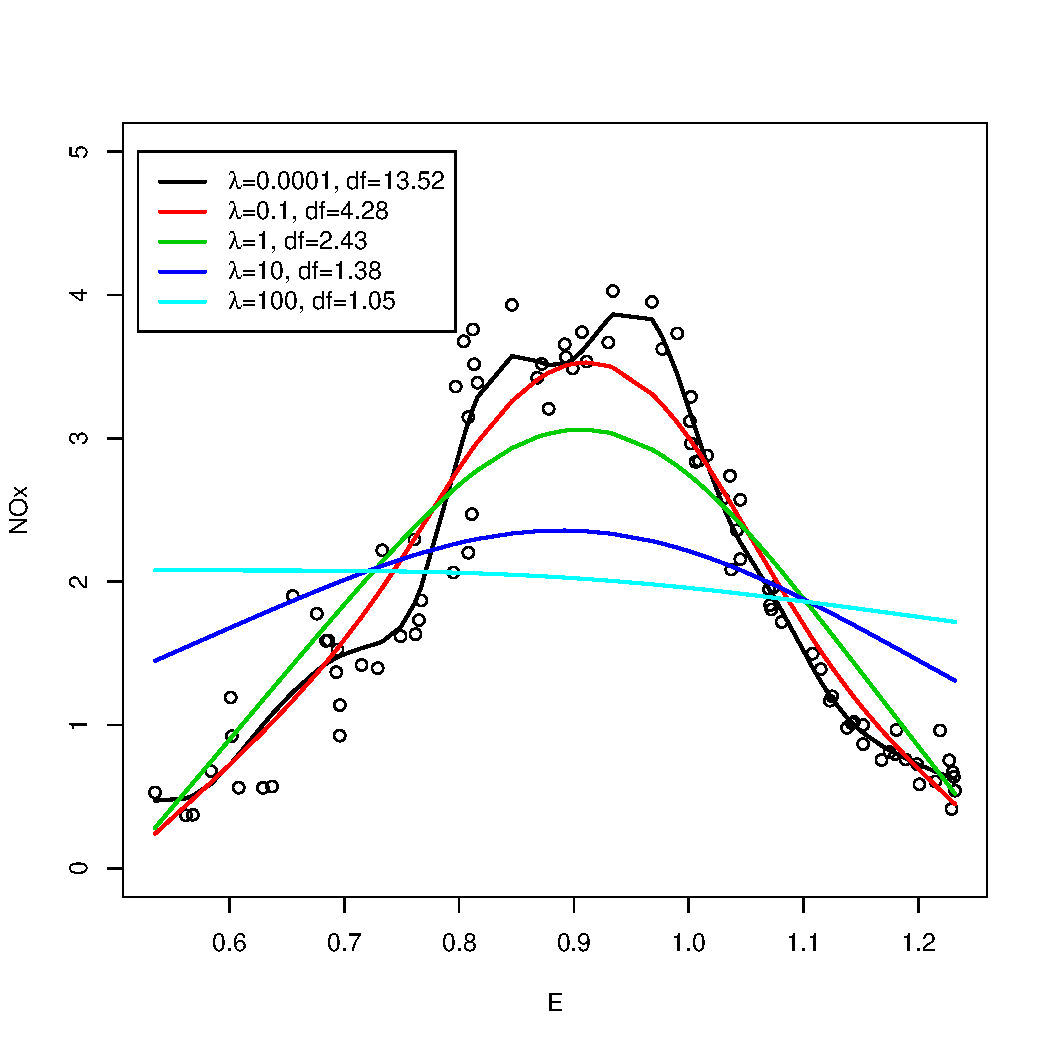
\includegraphics[width = 7.5cm]{figures/Ethanollambdaspline.pdf}  
\end{center}
\end{frame}


\begin{frame}
\frametitle{Choice of $\lambda$? }

Ideally, choose $\lambda$ so that $\hat{f}$ is as close as possible to $f$, by minimizing, for example,

$$M = \frac{1}{n} \sum_{i=1}^n \left( \hat{f}(x_i) - f(x_i) \right)^2.$$

\bigskip

But $f$ is unknown and $M$ cannot be used directly.
\end{frame}

\begin{frame}
\frametitle{Estimation of $M$ by cross-validation }

Define the ordinary cross-validation criterion
$$OCV(\lambda) = \frac{1}{n} \sum_{i=1}^n (y_i - \hat{f}^{-i}_{\lambda}(x_i))^2,$$
where $\hat{f}^{-i}_{\lambda} (x_i)$ indicates the fit at $x_i$ leaving out the
$i$th data point. It implies the fit of $n$ submodels.

\bs
It can be proven that $E(OCV) \approx E(M) + \sigma^2$.

\end{frame}

\begin{frame}
\frametitle{}

Because $\hat{y} = A y$ (see page~\pageref{linear.smoother})
$$OCV(\lambda) =  \frac{1}{n} \sum_{i=1}^n \Big(\frac{y_i -
  \hat{f}_{\lambda}(x_i)}{1-A_{ii}} \Big)^2,$$
which can be obtained from the fit of the full dataset only.

\bs
In practice, the $A_{ii}$ are often replaced by their average, giving the
generalized cross-validation criterion 
$$GCV(\lambda) =  \frac{1}{n} \sum_{i=1}^n \Big(\frac{y_i -
  \hat{f}_{\lambda}(x_i)}{1-Tr(A)/n} \Big)^2 = \frac{n \sum_{i=1}^n \Big(y_i -
  \hat{f}_{\lambda}(x_i)\Big)^2}{(n-Tr(A))^2}.$$

\bs
Note: $Tr(A) = Tr(F)$ because of the circularity of the trace.
\end{frame}

\begin{frame}
\frametitle{GCV for the ethanol dataset (spline basis)}

\vspace*{-0.5cm}
\begin{center}
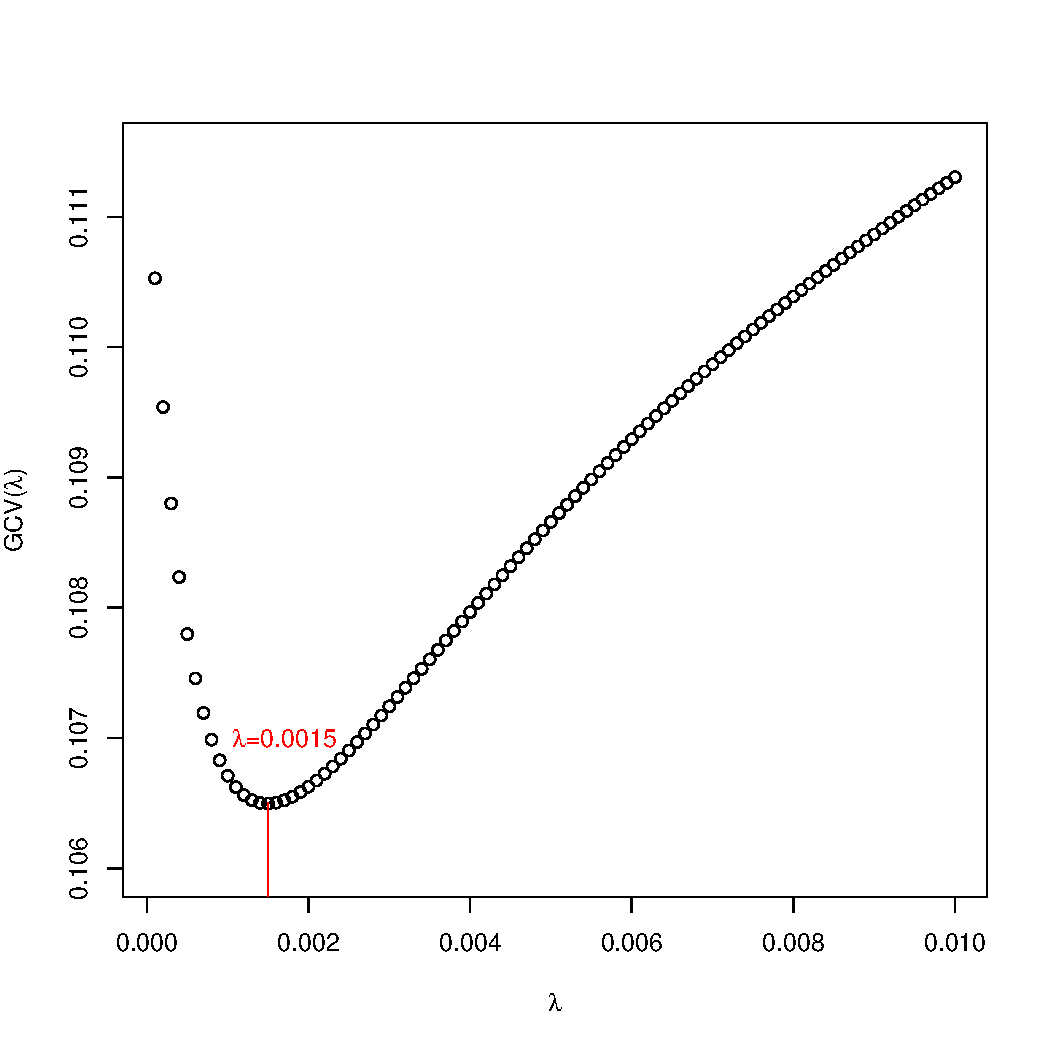
\includegraphics[width = 7.5cm]{figures/EthanolGCV.pdf}  
\end{center}
\end{frame}


\begin{frame}[fragile]
\frametitle{Ethanol automatic fit}

{\scriptsize
\begin{lstlisting}
> ethanol.gam <- gam(NOx~s(E,k=15),data=ethanol)

> ethanol.gam
Family: gaussian 
Link function: identity 

Formula:
NOx ~ s(E, k = 15)

Estimated degrees of freedom:
10.6  total = 11.63 

GCV score: 0.1064968 

> ethanol.gam$sp
       s(E) 
0.001490695   
\end{lstlisting}
}

\end{frame}

\begin{frame}[fragile]
\frametitle{Ethanol automatic fit}

{\tiny
\begin{lstlisting}
> summary(ethanol.gam)

Family: gaussian 
Link function: identity 

Formula:
NOx ~ s(E, k = 15)

Parametric coefficients:
            Estimate Std. Error t value Pr(>|t|)    
(Intercept)  1.95737    0.03241    60.4   <2e-16 ***
---
Signif. codes:  0 ‘***’ 0.001 ‘**’ 0.01 ‘*’ 0.05 ‘.’ 0.1 ‘ ’ 1

Approximate significance of smooth terms:
       edf Ref.df     F p-value    
s(E) 10.63  12.31 91.39  <2e-16 ***
---
Signif. codes:  0 ‘***’ 0.001 ‘**’ 0.01 ‘*’ 0.05 ‘.’ 0.1 ‘ ’ 1

R-sq.(adj) =  0.928   Deviance explained = 93.7%
GCV = 0.1065  Scale est. = 0.092419  n = 88
\end{lstlisting}
}

\end{frame}

\begin{frame}
\frametitle{Final fit}

\vspace*{-0.5cm}
\begin{center}
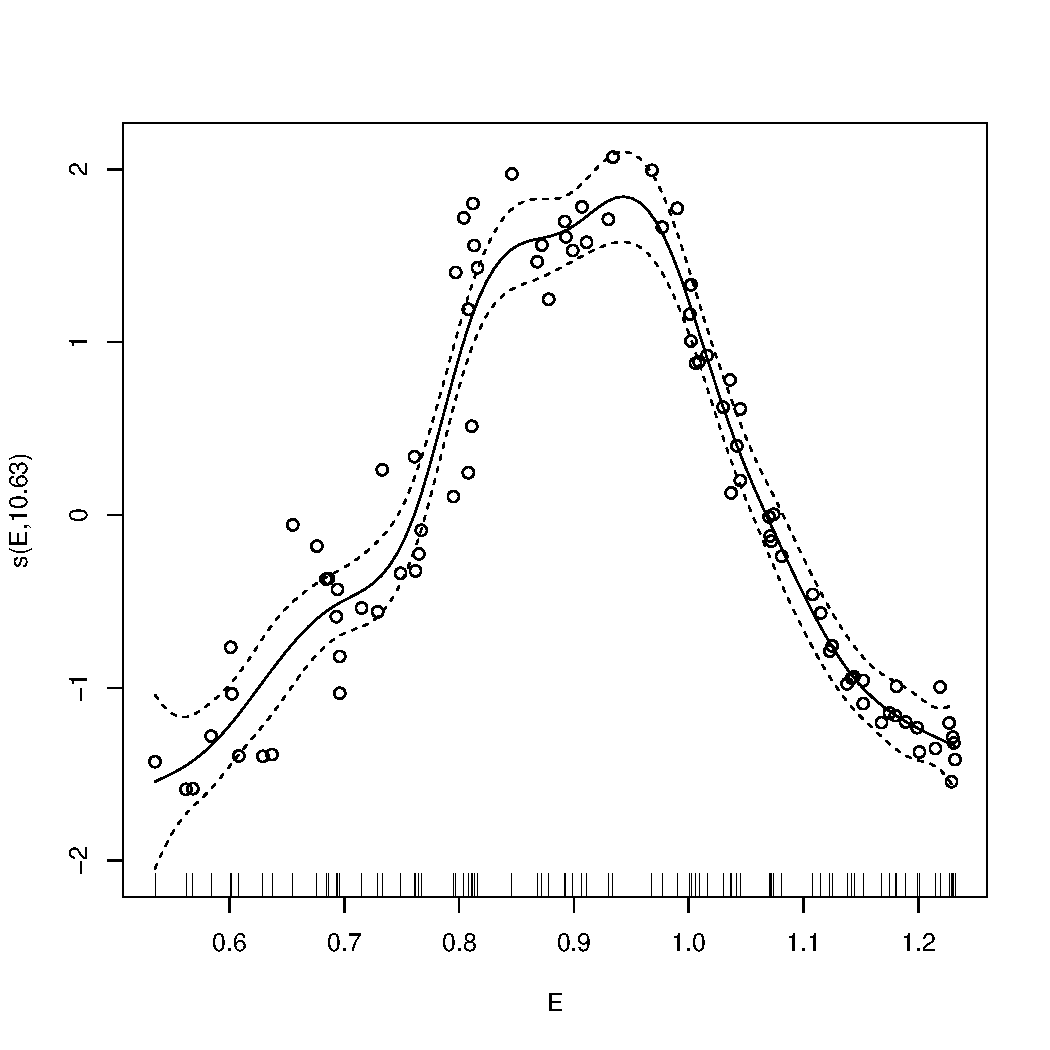
\includegraphics[width = 7.5cm]{figures/Ethanolfinal.pdf}  
\end{center}
\end{frame}

\subsection{Additive models}
\begin{frame}
\frametitle{Additive models - AM}
How do we go from 1 to $p$ predictors?

\bs
Ideally one should consider surface smoothers
$$y = f(x_1, \ldots, x_p) + \epsilon,$$
but with large $p$ this goal is out of reach.

\bs 
{\color{blue}Additive models} are an approximation:
$$y=\alpha+f_1(x_1) + f_2(x_2)+\ldots+f_p(x_p)+\epsilon,$$
with $E(\epsilon)=0$, $Var(\epsilon)=\sigma^2$ and $\epsilon$ independent of $x_j$.

\end{frame}


\begin{frame}
\frametitle{}

\bs
With more than one component, there is an identifiability problem: each function
$f_j$ is estimable only up to an additive constant. The constraint that 
$$\sum_{i=1}^n f_j(x_{ji})=0$$
for all $j$ is therefore added. 

\bs
Extensions of the simple additive model above can include component functions
with two or more dimensions, categorical variable terms and their interactions
with continuous variables.
\end{frame}

\begin{frame}
\frametitle{}
\textbf{Remarks}:
\begin{itemize} 
\item The additive form of the model allows the plotting of the $p$ functions
separately (better interpretability).
\item Additive models are more general approximations than linear regression models.
\item Additive fits can be helpful to test linearity.
\end{itemize}

\end{frame}


\begin{frame}
\frametitle{Fitting additive models}

We represent each function with basis functions such that $f_j(x_j) =
\sum_{k=1}^K b_k(x_j) \delta_k^{(j)}$. The model is
$$y_i = \alpha+ \sum_{j=1}^p f_j(x_{ji}) +\epsilon_i = \alpha+ \sum_{j=1}^p X^{(j)} \delta^{(j)} +\epsilon_i,$$
where $X^{(j)}$ contains the basis function for covariate $j$. 

\bs 
Define the associated penalties $(\delta^{(j)})^T \bar{S}_j \delta^{(j)}$ and $X
= [1 \  X^{(1)}  \ldots  \ X^{(p)} ]$. Consider also the vector of all the
parameters $\beta = (\alpha, \delta^{(1)}, \ldots, \delta^{(p)})^T$.
\end{frame}



\begin{frame}
\frametitle{}
We now solve
 $$\hat{\beta} = \mbox{argmin}_{\beta} \{  ||y - X \beta ||^2 + \sum_{j=1}^{p} \lambda_j  \beta^T S_j \beta \},$$
where $S_j$ is constructed with $\bar{S}_j$ and padded out with zeros such that
$(\delta^{(j)})^T \bar{S}_j \delta^{(j)} = \beta^T S_j \beta$.

\bs
Similarly to the univariate case, we have
$$\hat{\beta} = (X^T X + \lambda_1 S_1 + \ldots + \lambda_p S_p)^{-1} X^T y,$$
$$A = X (X^T X + \lambda_1 S_1 + \ldots + \lambda_p S_p)^{-1} X^T,$$
and
$$F = (X^T X + \lambda_1 S_1 + \ldots + \lambda_p S_p)^{-1} X^T X .$$
\end{frame}


\begin{frame}
\frametitle{}
For computational stability, the corresponding augmented problem is considered:
\begin{eqnarray*}
& & \left|\left| y - X \beta \right|\right|^2 + \beta^T (\lambda_1 S_1 +
\ldots + \lambda_p S_p) \beta \\
& & = \left|\left|
\left(\begin{array}{c}
y \\
0
\end{array} \right) -
\left(\begin{array}{c}
X \\
B
\end{array} \right) \beta
\right|\right|^2,
\end{eqnarray*}
where $B$ is such that $B^T B = \lambda_1 S_1 + \ldots + \lambda_p S_p.$

\bs
It is a least squares problem.
\end{frame}

\begin{frame}
\frametitle{Choice of $(\lambda_1, \ldots, \lambda_p)$ by GCV}

Find $(\lambda_1, \ldots, \lambda_p)$ that minimizes
\begin{eqnarray}
GCV(\lambda_1, \ldots, \lambda_p) & = &   \frac{1}{n} \sum_{i=1}^n \Big(\frac{y_i -
  \hat{f}_{\lambda_1, \ldots, \lambda_p}(x_i)}{1-Tr(A)/n} \Big)^2 \\
  & = &  \frac{n \sum_{i=1}^n \Big(y_i -
  \hat{f}_{\lambda_1, \ldots, \lambda_p}(x_i)\Big)^2}{(n-Tr(A))^2}.
\end{eqnarray}

\end{frame}



\begin{frame}
\frametitle{Posterior distribution for $\beta$}
We have
$$ \beta | y \sim {\mathcal N}(\hat{\beta}, V_{\beta}),$$
where $V_{\beta} = \sigma^2 (X^T X + \lambda_1 S_1 + \ldots + \lambda_p S_p)$.

\bs 
$V_{\beta}$ is estimated by plugging in $\hat{\sigma}^2 = ||y - X
\hat{\beta}||^2/ (n - Tr(F))$. 

\bs
The above result can be used for inference on $\beta$, either directly (quantities linear in the model parameters) or by simulation or bootstrap (in other cases).
\end{frame}

\begin{frame}
\frametitle{Hypothesis testing on $\beta$}
Suppose we want to test $H_0: \beta_j=0$, where $\beta_j$ is a subvector of size
$p_j$ of 
$\beta$. Let $V_{\beta_j}$ denote the block of $V_{\beta}$ corresponding to
$\beta_j$. 

\bs
Then, under $H_0$  one can use the test statistics
$$\hat{\beta_j}^T V_{\beta_j}^{-1} \hat{\beta_j}/p_j \sim F_{p_j,n-p},$$
if there is a scale parameter involved ($\phi$ unknown), and 
$$\hat{\beta_j}^T V_{\beta_j}^{-1} \hat{\beta_j} \sim \chi_{p_j}^2,$$
if not  ($\phi$ known).
\end{frame}

\begin{frame}
\frametitle{Confidence intervals for $f_j$}

From the posterior distribution of $\beta$, credible intervals can be constructed for $f_j$. 

\bs
Let $\tilde{f}_j = \tilde{X} \beta$, where $\tilde{X}$ has zeros in the columns corresponding to the coefficients having nothing to do with $f_j$, while its other columns contain the basis functions for $f_j$. Let $v= \mbox{diag}(\tilde{X} V_{\beta} \tilde{X}^T)$, then
$$\hat{f_{ji}} \pm z_{\alpha/2} \sqrt{v_i}$$
is an approximate $(1-\alpha) 100 \%$  credible interval for $f_{ji}$.

\bs
It turns out that Bayesian credible intervals have good frequentist coverage properties.

\end{frame}


\begin{frame}
\frametitle{Variable selection for smooth terms}
A test statistics can be derived to test the null hypothesis $H_0:
f_j(x_j)=0$. Let $f_j = \tilde{X} \beta$. Then, from $\hat{\beta} \sim {\mathcal
N}(\beta, V_{\beta})$, we have $ \hat{f_j} \sim {\mathcal N}(f_j,  V_{f_j}),$
where $V_{f_j} = \tilde{X}  V_{\beta} \tilde{X}^T$.

\bs
The test statistics is defined by
$$ T_r = \hat{f_j}^T V_{f_j}^{r -} \hat{f_j} ,$$
where $V_{f_j}^{r -}$ is a rank $r$ pseudo-inverse of $V_{f_j}$.

\bs
Some care has to be taken for the choice of $r$. In a nutshell, this choice is done based on the estimated degrees of freedom of the function of $f_j$.

\bs
The distribution of $T_r$ under $H_0$ is $\chi^2_r$ if $r$ is integer.
\end{frame}

\begin{frame}[fragile]
\frametitle{Boston housing data analysis}

{\tiny
\begin{lstlisting}
> BHnpfit <- gam(log(medv)~chas+s(crim)+s(zn)+s(indus)+s(nox)+s(rm)+s(age)+s(dis)+
   s(rad,k=8)+s(tax)+s(ptratio)+s(b)+s(lstat),data=BostonHousing)
> BHnpfit

Family: gaussian 
Link function: identity 

Formula:
log(medv) ~ chas + s(crim) + s(zn) + s(indus) + s(nox) + s(rm) + 
    s(age) + s(dis) + s(rad, k = 8) + s(tax) + s(ptratio) + s(b) + 
    s(lstat)

Estimated degrees of freedom:
3.12 1.00 7.83 9.00 4.59 1.00 8.61 
1.33 3.09 1.00 4.99 5.24  total = 52.8 

GCV score: 0.02158189     
\end{lstlisting}
}

\end{frame}

\begin{frame}[fragile]
\frametitle{}
{\tiny
\begin{lstlisting}
> gam.check(BHnpfit)

Method: GCV   Optimizer: magic
Smoothing parameter selection converged after 20 iterations.
The RMS GCV score gradient at convergence was 2.97197e-08 .
The Hessian was positive definite.
Model rank =  108 / 108 

Basis dimension (k) checking results. Low p-value (k-index<1) may
indicate that k is too low, especially if edf is close to k'.

              k'   edf k-index p-value
s(crim)    9.000 3.123   1.074    0.94
s(zn)      9.000 1.000   0.797    0.00
s(indus)   9.000 7.825   0.790    0.00
s(nox)     9.000 9.000   0.838    0.00
s(rm)      9.000 4.591   0.941    0.10
s(age)     9.000 1.000   0.974    0.23
s(dis)     9.000 8.613   0.936    0.08
s(rad)     7.000 1.330   0.796    0.00
s(tax)     9.000 3.089   0.798    0.00
s(ptratio) 9.000 1.000   0.814    0.00
s(b)       9.000 4.989   0.981    0.34
s(lstat)   9.000 5.240   1.072    0.94
\end{lstlisting}
}
\end{frame}

\begin{frame}[fragile]
\frametitle{}

{\tiny
\begin{lstlisting}
> BHnpfit.new <- gam(log(medv)~chas+s(crim)+s(zn)+s(indus)+s(nox,k=20)+s(rm)+s(age)+
    s(dis,k=20)+s(rad,k=8)+s(tax)+s(ptratio)+s(b)+s(lstat),data=BostonHousing)
> BHnpfit.new

Family: gaussian 
Link function: identity 

Formula:
log(medv) ~ chas + s(crim) + s(zn) + s(indus) + s(nox, k = 20) + 
    s(rm) + s(age) + s(dis, k = 20) + s(rad, k = 8) + s(tax) + 
    s(ptratio) + s(b) + s(lstat)

Estimated degrees of freedom:
 3.37  1.00  5.21 13.07  5.10  1.00 13.40 
 2.26  3.20  1.00  1.94  4.76  total = 57.3 

GCV score: 0.02116857 
\end{lstlisting}
}
\end{frame}
 

\begin{frame}[fragile]
\frametitle{}

{\tiny
\begin{lstlisting}
> gam.check(BHnpfit.new)

Method: GCV   Optimizer: magic
Smoothing parameter selection converged after 21 iterations.
The RMS GCV score gradient at convergence was 2.186018e-08 .
The Hessian was positive definite.
Model rank =  128 / 128 

Basis dimension (k) checking results. Low p-value (k-index<1) may
indicate that k is too low, especially if edf is close to k'.

               k'    edf k-index p-value
s(crim)     9.000  3.368   1.078    0.94
s(zn)       9.000  1.000   0.838    0.00
s(indus)    9.000  5.211   0.819    0.00
s(nox)     19.000 13.065   0.875    0.00
s(rm)       9.000  5.101   0.948    0.14
s(age)      9.000  1.000   0.990    0.40
s(dis)     19.000 13.397   0.967    0.20
s(rad)      7.000  2.260   0.835    0.00
s(tax)      9.000  3.202   0.834    0.00
s(ptratio)  9.000  1.000   0.856    0.00
s(b)        9.000  1.945   0.978    0.34
s(lstat)    9.000  4.755   1.077    0.94
\end{lstlisting}
}
\end{frame}

\begin{frame}
\frametitle{}

\vspace*{-0.5cm}
\begin{center}
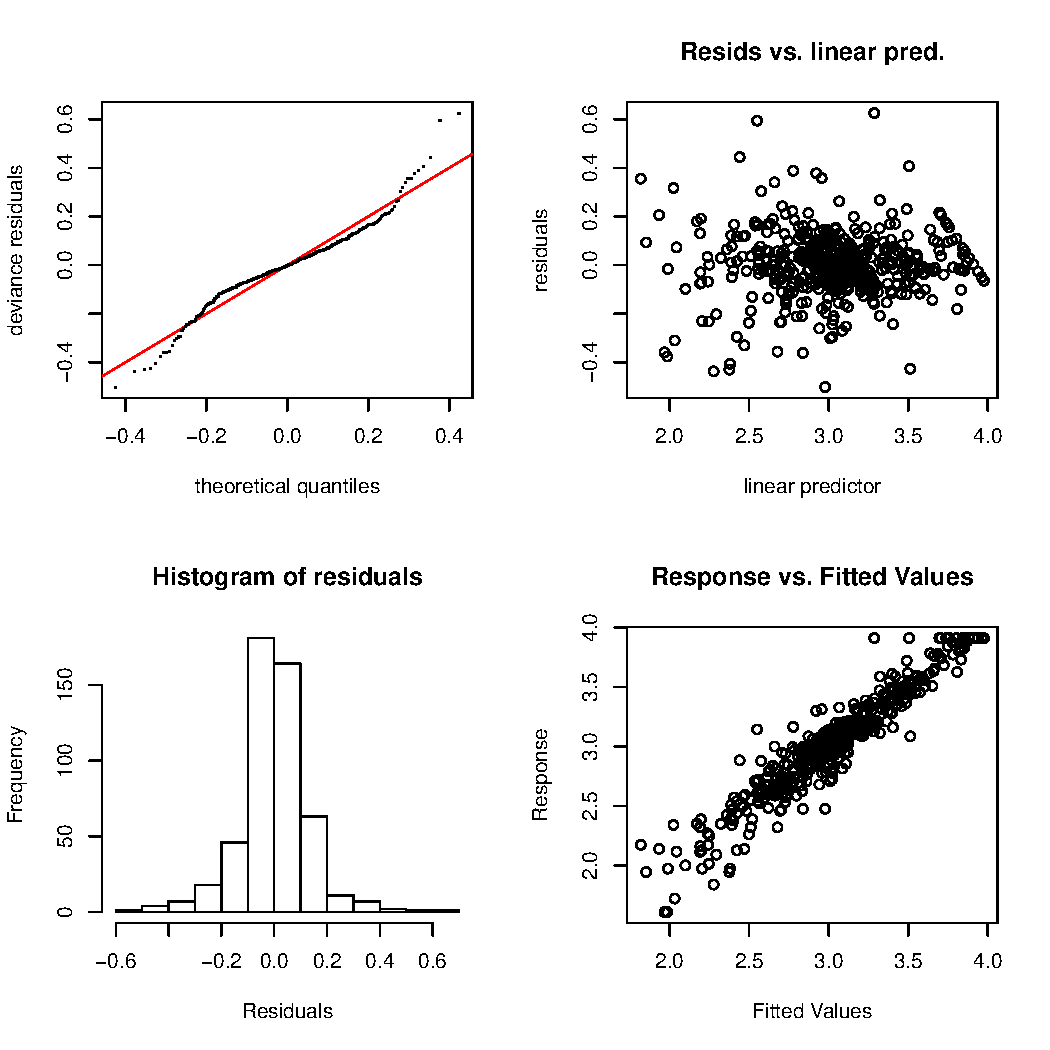
\includegraphics[width = 7.5cm]{figures/BHnpfitnewCheck.pdf}  
\end{center}
\end{frame}

\begin{frame}[fragile]
\frametitle{}

{\tiny
\begin{lstlisting}
Family: gaussian 
Link function: identity 
Formula: log(medv) ~ chas + s(crim) + s(zn) + s(indus) + s(nox, k = 20) +  s(rm) + s(age) + 
  s(dis, k = 20) + s(rad, k = 8) + s(tax) +  s(ptratio) + s(b) + s(lstat)

Parametric coefficients:
            Estimate Std. Error t value Pr(>|t|)    
(Intercept) 3.031791   0.006376 475.497   <2e-16 ***
chas        0.039350   0.027264   1.443     0.15    
---
Signif. codes:  0 ‘***’ 0.001 ‘**’ 0.01 ‘*’ 0.05 ‘.’ 0.1 ‘ ’ 1

Approximate significance of smooth terms:
              edf Ref.df      F  p-value    
s(crim)     3.368  4.184 19.183 7.60e-15 ***
s(zn)       1.000  1.000  0.639  0.42437    
s(indus)    5.211  6.119  1.882  0.08638 .  
s(nox)     13.065 15.171 11.476  < 2e-16 ***
s(rm)       5.101  6.262 17.018  < 2e-16 ***
s(age)      1.000  1.000  1.964  0.16174    
s(dis)     13.397 15.676  3.900 9.16e-07 ***
s(rad)      2.260  2.627 10.931 4.05e-06 ***
s(tax)      3.202  3.789 11.648 1.24e-08 ***
s(ptratio)  1.000  1.000 37.846 1.63e-09 ***
s(b)        1.945  2.401  5.254  0.00327 ** 
s(lstat)    4.755  5.864 35.015  < 2e-16 ***
---
Signif. codes:  0 ‘***’ 0.001 ‘**’ 0.01 ‘*’ 0.05 ‘.’ 0.1 ‘ ’ 1

R-sq.(adj) =  0.888   Deviance explained =   90%
GCV = 0.021169  Scale est. = 0.018771  n = 506
\end{lstlisting}
}

\end{frame}

\begin{frame}
\frametitle{}

\vspace*{-0.5cm}
\begin{center}
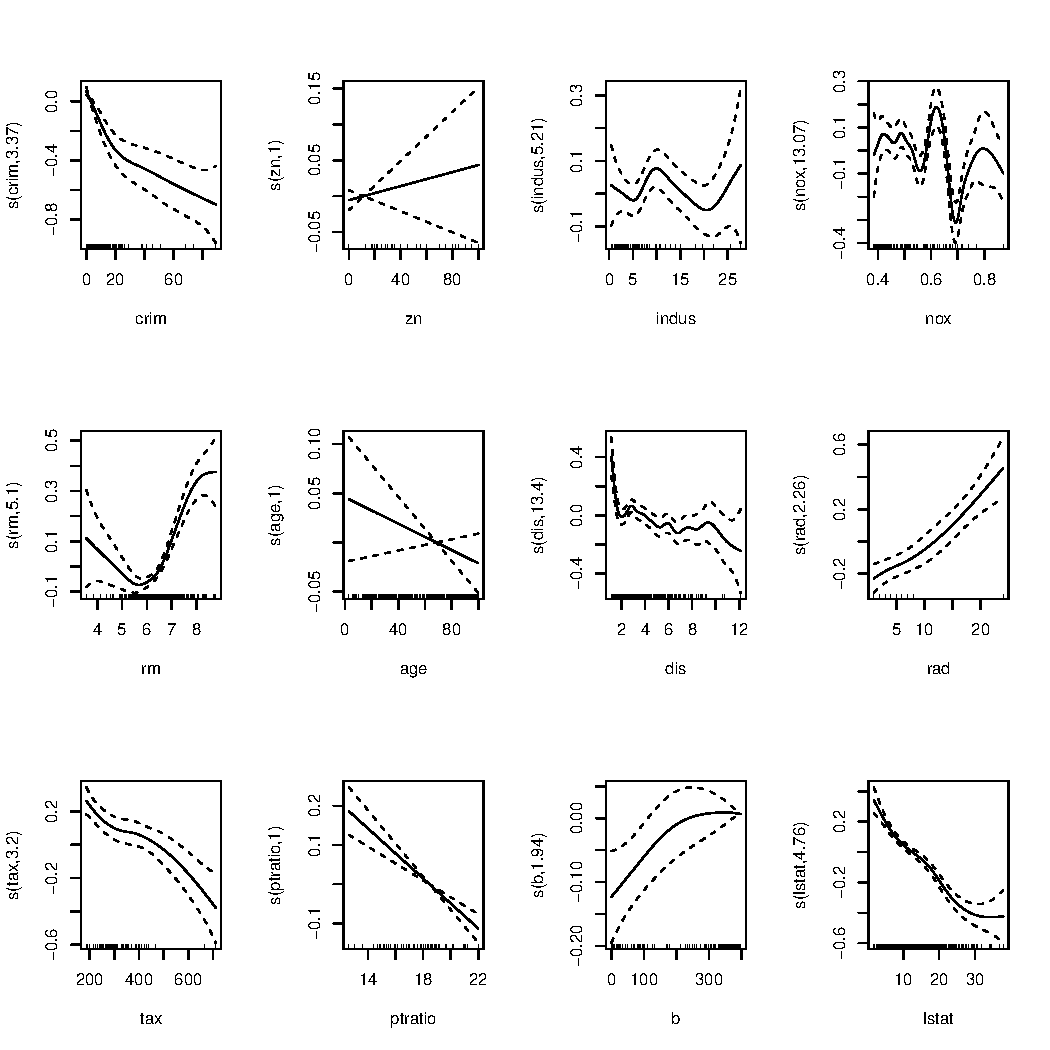
\includegraphics[width = 8cm]{figures/BHnpfitnew.pdf}  
\end{center}
\end{frame}

\begin{frame}[fragile]
\frametitle{Remove \texttt{zn}, \texttt{age} and \texttt{chas}?}

{\tiny
\begin{lstlisting}
> BHnpfit2.new <- gam(log(medv)~s(crim)+s(indus)+s(nox,k=20)+s(rm)+s(dis,k=20)+
   s(rad,k=8)+s(tax)+s(ptratio)+s(b)+s(lstat),data=BostonHousing)
> BHnpfit2.new

Family: gaussian 
Link function: identity 

Formula: log(medv) ~ s(crim) + s(indus) + s(nox, k = 20) + s(rm) + s(dis, k = 20) + 
   s(rad, k = 8) + s(tax) + s(ptratio) + s(b) + s(lstat)

Estimated degrees of freedom:
 3.35  5.12 12.79  4.96 13.33  2.35  3.27 
 1.00  1.91  4.83  total = 53.92 

GCV score: 0.02112012 
\end{lstlisting}
}

\end{frame}


\begin{frame}[fragile]
\frametitle{}

{\tiny
\begin{lstlisting}
> gam.check(BHnpfit2.new)

Method: GCV   Optimizer: magic
Smoothing parameter selection converged after 20 iterations.
The RMS GCV score gradient at convergence was 4.284208e-08 .
The Hessian was positive definite.
Model rank =  109 / 109 

Basis dimension (k) checking results. Low p-value (k-index<1) may
indicate that k is too low, especially if edf is close to k'.

               k'    edf k-index p-value
s(crim)     9.000  3.352   1.082    0.96
s(indus)    9.000  5.123   0.813    0.00
s(nox)     19.000 12.795   0.876    0.00
s(rm)       9.000  4.961   0.940    0.08
s(dis)     19.000 13.325   0.967    0.22
s(rad)      7.000  2.353   0.828    0.00
s(tax)      9.000  3.268   0.823    0.00
s(ptratio)  9.000  1.000   0.849    0.00
s(b)        9.000  1.915   0.987    0.44
s(lstat)    9.000  4.828   1.076    0.96
\end{lstlisting}
}

\end{frame}

\begin{frame}
\frametitle{}

\vspace*{-0.5cm}
\begin{center}
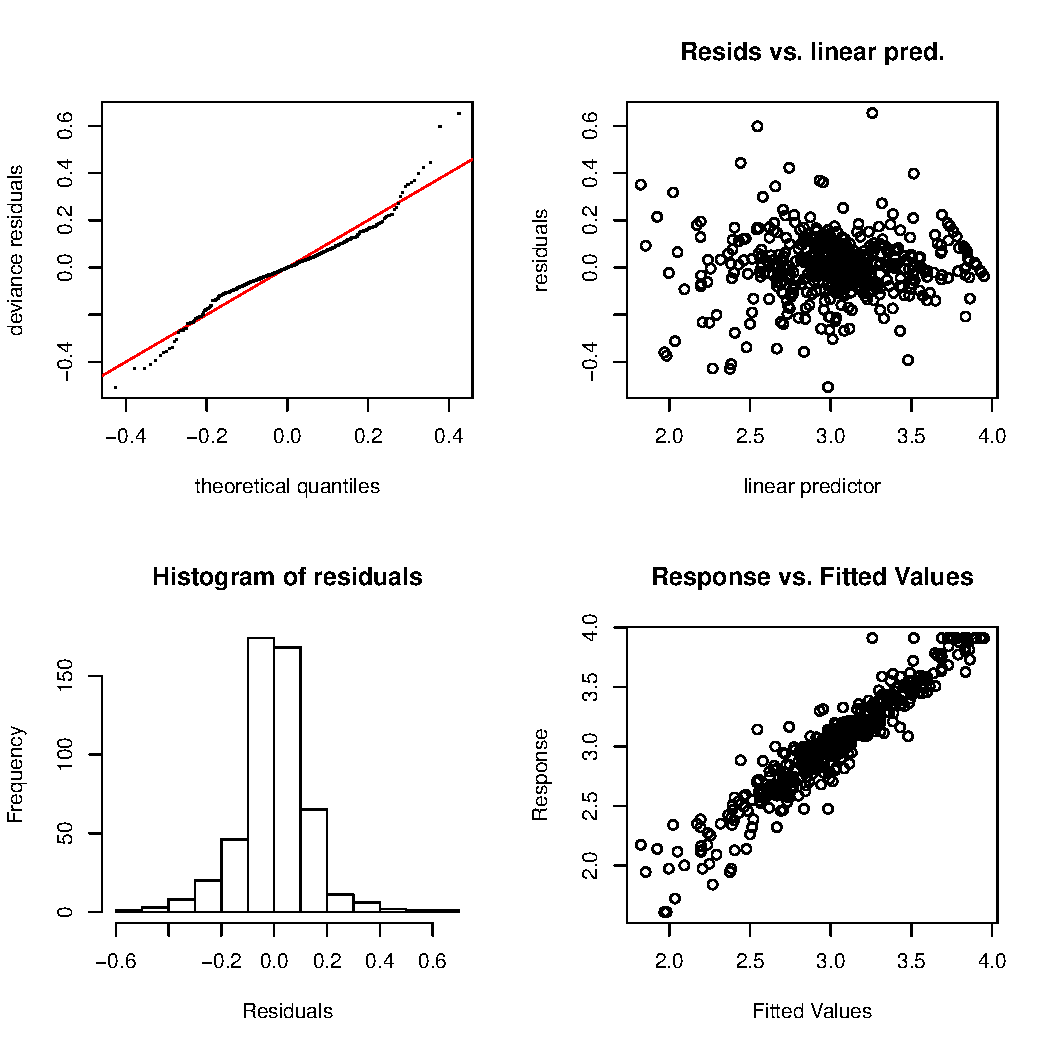
\includegraphics[width = 7.5cm]{figures/BHnpfitnew2Check.pdf}  
\end{center}
\end{frame}

\begin{frame}[fragile]
\frametitle{}

{\tiny
\begin{lstlisting}
> summary(BHnpfit2.new)

Family: gaussian 
Link function: identity 

Formula: log(medv) ~ s(crim) + s(indus) + s(nox, k = 20) + s(rm) + s(dis, k = 20) + 
   s(rad, k = 8) + s(tax) + s(ptratio) + s(b) + s(lstat)

Parametric coefficients:
            Estimate Std. Error t value Pr(>|t|)    
(Intercept) 3.034513   0.006107   496.9   <2e-16 ***
---
Signif. codes:  0 ‘***’ 0.001 ‘**’ 0.01 ‘*’ 0.05 ‘.’ 0.1 ‘ ’ 1

Approximate significance of smooth terms:
              edf Ref.df      F  p-value    
s(crim)     3.352  4.165 19.885 2.34e-15 ***
s(indus)    5.123  6.030  2.132  0.04962 *  
s(nox)     12.795 14.900 11.670  < 2e-16 ***
s(rm)       4.961  6.109 17.497  < 2e-16 ***
s(dis)     13.325 15.611  3.932 6.55e-07 ***
s(rad)      2.353  2.735 11.034 2.13e-06 ***
s(tax)      3.268  3.868 11.418 1.14e-08 ***
s(ptratio)  1.000  1.000 44.876 5.87e-11 ***
s(b)        1.915  2.365  5.030  0.00437 ** 
s(lstat)    4.828  5.938 43.788  < 2e-16 ***
---
Signif. codes:  0 ‘***’ 0.001 ‘**’ 0.01 ‘*’ 0.05 ‘.’ 0.1 ‘ ’ 1

R-sq.(adj) =  0.887   Deviance explained = 89.9%
GCV = 0.02112  Scale est. = 0.01887   n = 506
\end{lstlisting}
}
\end{frame}

\begin{frame}
\frametitle{}

\vspace*{-0.5cm}
\begin{center}
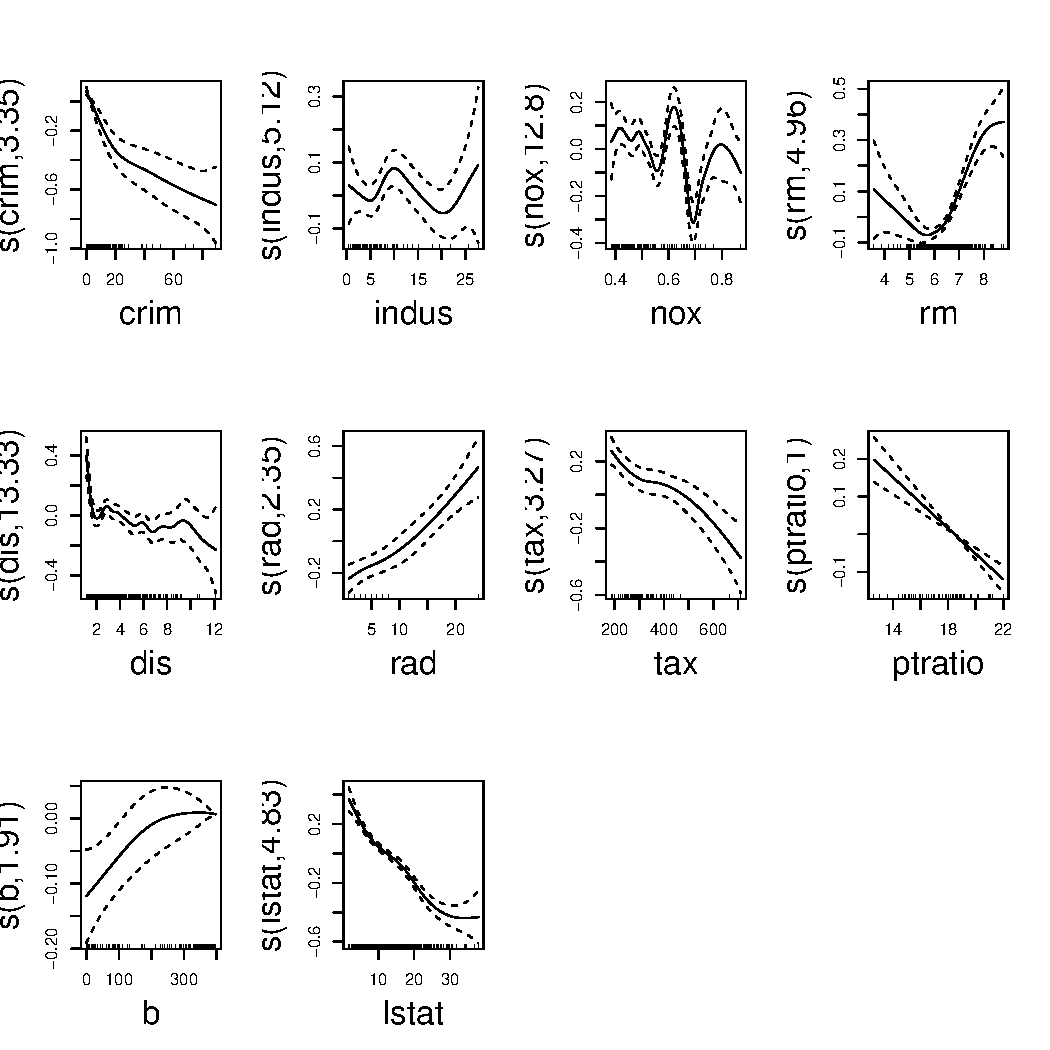
\includegraphics[width = 8cm]{figures/BHnpfit2new.pdf}  
\end{center}
\end{frame}


\begin{frame}[fragile]
\frametitle{Remove \texttt{ptratio}?}

{\tiny
\begin{lstlisting}
> BHnpfit3.new <- gam(log(medv)~s(crim)+s(indus)+s(nox,k=20)+s(rm)+s(dis,k=20)+s(rad,k=8)
+s(tax)+s(b)+s(lstat),data=BostonHousing)
> BHnpfit3.new

Family: gaussian 
Link function: identity 

Formula:
log(medv) ~ s(crim) + s(indus) + s(nox, k = 20) + s(rm) + s(dis, 
    k = 20) + s(rad, k = 8) + s(tax) + s(b) + s(lstat)

Estimated degrees of freedom:
 3.35  8.10 13.58  5.30 12.33  1.00  3.27 
 1.77  4.70  total = 54.39 

GCV score: 0.02258293   

> BHnpfit3.new$aic
[1] -486.3607
\end{lstlisting}
}

The Akaike value of this model is -486.36, much worst of what we had before.
\end{frame}


\subsection{Generalized additive models}

\begin{frame}
\frametitle{GAM ingredients}

\begin{enumerate}
\item Independent response variables $Y_1, \ldots,Y_n$ which are assumed to share
  the same distribution from the {\color{blue}exponential family} ($F_{\theta_i}$).
\item A set of {\color{blue}explanatory variables}\\
 $x_i^T = (x_{i1},  \ldots, x_{ip})$ for $i=1,\ldots,n$.
\item A monotone {\color{blue}link} function $g$ such that
$$g(\mu_i) = \alpha + f_1(x_{i1}) + \ldots + f_p(x_{ip}) = \eta_i.$$
$\eta_i $ is called the {\color{blue}additive predictor}.
\end{enumerate}

\bs
We assume that
$$E(Y_i) = \mu_i \ \mbox{and} \ \ Var(Y_i) = v_i = v(\mu_i).$$
The difference with the GLM model is the fact that $\mu_i$ is obtained
nonparametrically, via $g^{-1}(\alpha + f_1(x_{i1}) + \ldots + f_p(x_{ip}))$.
\end{frame}

\begin{frame}
\frametitle{}
We now have
$$g(\mu_i ) =  \alpha+ \sum_{j=1}^p f_j(x_{ji}) = \alpha+ \sum_{j=1}^p X^{(j)} \delta^{(j)},$$
with associated penalties $(\delta^{(j)})^T \bar{S}_j \delta^{(j)}$ and $X
= [1 \  X^{(1)}  \ldots  \ X^{(p)} ]$. 

\bigskip 
Consider $\beta = (\alpha, \delta^{(1)}, \ldots, \delta^{(p)})$. We solve
 $$\hat{\beta} = \mbox{argmin}_{\beta} \{  D(y,\mu)+ \sum_{j=1}^{p} \lambda_j  \beta^T S_j \beta \},$$
where $D(y,\mu)$ is the deviance function (see p.~\pageref{deviance.def}) and  where $S_j$ is constructed with $\bar{S}_j$ and padded out with zeros such that
$(\delta^{(j)})^T \bar{S}_j \delta^{(j)} = \beta^T S_j \beta$.
\end{frame}

\begin{frame}
\frametitle{}
GAM are fitted with a {\color{blue}local scoring algorithm}.

\bigskip
At step $(m-1)$, construct an {\color{blue}adjusted dependent variable}
$$z_i^{(m-1)} = \eta_i^{(m-1)} + (y_i - \mu_i^{(m-1)}) \Big(\frac{\partial \eta_i}{\partial \mu_i} \Big)^{(m-1)},$$
with $\eta_i^{(m-1)} = \alpha^{(m-1)} + \sum_{j=1}^p f_j^{(m-1)}(x_{ij})$, and weights
$$w_i^{(m-1)} = \frac{1}{Var(Y_i)^{(m-1)}}\Big(\frac{\partial \mu_i}{\partial \eta_i} \Big)_{(m-1)}^2.$$

Fit a {\color{blue}weighted additive model} to $z_i^{(m-1)}$ to obtain estimated functions $f_j^{(m)}$, additive predictor $\eta_i^{(m)}$, and fitted values $\mu_i^{(m)}$. Repeat until convergence is reached.


\bs
The weighted least squares fit of GLM in the local scoring
algorithm is replaced by a weighted additive fit (see page~\pageref{IWLSweights}).

\end{frame}


\begin{frame}
\frametitle{}
The weighted additive fit can be written as a weighted least squares fit for the augmented problem as follow:
$$\left|\left|
\left(\begin{array}{cc}
\sqrt{W^{(m-1)}} & 0 \\
0 & I 
\end{array} \right) 
\left[
\left(\begin{array}{c}
z^{(m-1)} \\
0
\end{array} \right) -
\left(\begin{array}{c}
X \\
B
\end{array} \right) \right]\beta
\right|\right|^2,
$$
with $W^{(m-1)} = \mbox{diag}(w_1^{(m-1)}, \ldots,w_n^{(m-1)})$ and $B$ is such that $B^T B = \lambda_1 S_1 + \ldots + \lambda_p S_p.$

\end{frame}

\begin{frame}
\frametitle{Properties}

The effective degrees of freedom matrix becomes
$$F = (X^T  WX + \lambda_1 S_1 + \ldots + \lambda_p S_p)^{-1} X^T W X .$$

\bigskip
It holds asymptotically that
$$ \beta | y \sim {\mathcal N}(\hat{\beta}, V_{\beta}),$$
where $V_{\beta} = \sigma^2 (X^T W X + \lambda_1 S_1 + \ldots + \lambda_p S_p)$.

\bigskip
The scale parameter, if unknown, is estimated by
$\hat{\phi} = \sum_{i=1}^n (y_i - X_i \hat{\beta})^2/ (n - Tr(F))$. 

\end{frame}


\begin{frame}
\frametitle{Choice of $\lambda_1,\ldots,\lambda_p$ for $\phi$ known}

Minimize mean squared error:

\bs
For an additive model with constant variance, it holds
\begin{eqnarray*}
M(\lambda_1,\ldots,\lambda_p) & = &  E \left( \frac{ \left|\left| \mu - X \hat{\beta}  \right|\right|^2}{n} \right) \\
& = & E \left( \frac{ \left|\left| y - A y  \right|\right|^2}{n} \right) - \phi + \frac{2 \phi Tr(A)}{n},  
\end{eqnarray*}
(see p.~52 and p.~255 in \citeN{Wood:2017} on how to obtain the last expression.)

\end{frame}


\begin{frame}
\frametitle{}
The form of $M$ suggests the following estimator (Un-Biased Risk Estimator)
$$ UBRE(\lambda_1,\ldots,\lambda_p) = \frac{ \left|\left| y - Ay  \right|\right|^2}{n}   - \phi + \frac{2 \phi Tr(A)}{n} = D(y,\hat{\mu}) + \frac{2 \phi Tr(F)}{n}.$$
which is also known as Mallows' $C_p$.

\bs 
UBRE has to be miminized.

\bs
By extension, it is used for all the families with $\phi$ known.
\end{frame}

\begin{frame}
\frametitle{Choice of $\lambda$ for $\phi$ unknown}

If $\phi$ unknown, it has to be estimated. Plugging-in $\hat{\phi}$ in the UBRE defintion makes it unsuitable for model selection.

\bs
Therefore, $GCV$ is used. It generalizes to 
$$ GCV(\lambda_1, \ldots,\lambda_p) = \frac{n D(y,\hat{\mu})}{(n- Tr(F))^2}.$$
\end{frame}

\begin{frame}
\frametitle{Model validation}

\begin{itemize}
\item Informal checks on $K$  
\item[]
\item Residuals analysis
\end{itemize}

\end{frame}

\begin{frame}
\frametitle{Comparing (nested) models}

Being in a likeihood framework, the Akaike criterion can be used to compare nested models:
$$AIC = -2 l(\hat{\beta};y) + 2 \phi Tr(F).$$
Models with smallest $AIC$ have to be preferred.

\bs
$GCV(\hat{\lambda}_1, \ldots,\hat{\lambda}_p)$  estimates the prediction
error. It can be used to compare models. Models with smallest $GCV$ have to be preferred.

\bs
The proportion of deviance explained is also a measure of the quality of a fit.

\end{frame}

\subsection{Analysis of the birds dataset}
\begin{frame}
\frametitle{Analysis of the birds dataset}

Outcome: Number of birds observed (counts, \texttt{NUMBER}).

\bs
Predictors:
\begin{itemize}
\item year (\texttt{YEAR})  - {\color{blue}Main interest}.
\item day (\texttt{DAY}) 
\item number
of observer on the island (\texttt{NO.OBS}) 
\item wind direction at midnight the night before (\texttt{WIND.0}) 
\item wind direction at noon the day before (\texttt{WIND.1}) 
\item wind direction at midnight 2 days before (\texttt{WIND.2}) 
\item wind direction at noon 2 days before (\texttt{WIND.3}) 
\item the speed of the wind that day (\texttt{WINDSPD}) 
\item sky condition (1=clear, 2=cloudy, 3=fog, 4=rain) (\texttt{SKY})
\item proportion of illuminated moon (\texttt{MOON}) 
\item bird species (1-5) (\texttt{BIRD})
\end{itemize}

\end{frame}


\begin{frame}[fragile]
\frametitle{Poisson model with logarithmic link}

\begin{eqnarray*}
\lefteqn{\texttt{NUMBER} \sim  \alpha + f_1(\texttt{YEAR}) + f_2(\texttt{DAY}) +
f_3(\texttt{NO.OBS})} \\
& + & f_4(\texttt{WIND.0}) + f_5(\texttt{WIND.1}) +
f_6(\texttt{WIND.2}) \\
& + & f_7(\texttt{WIND.3}) + f_8(\texttt{WINDSPD}) +
\mbox{factor(\texttt{SKY})}\\
& + & f_9(\texttt{MOON}) + \mbox{factor}(\texttt{BIRD})
\end{eqnarray*}

\bs

{\scriptsize
\begin{lstlisting}
> require(mgcv)
> GrA.fit <- gam(NUMBER~s(YEAR,k=20)+s(DAY,k=20)+s(NO.OBS,k=8)+
   s(WIND.0,k=20)+s(WIND.1,k=20)+s(WIND.2,k=20)+s(WIND.3,k=20)+
   s(WINDSPD,k=20)+factor(SKY)+s(MOON,k=20)+factor(BIRD), 
   family=poisson,data=GrA,na.action=na.omit)
> plot(GrA.fit,scale=0,pages=1,pers=T,cex.lab=2)
\end{lstlisting}
}
\end{frame}

\begin{frame}
\frametitle{}

\begin{center}
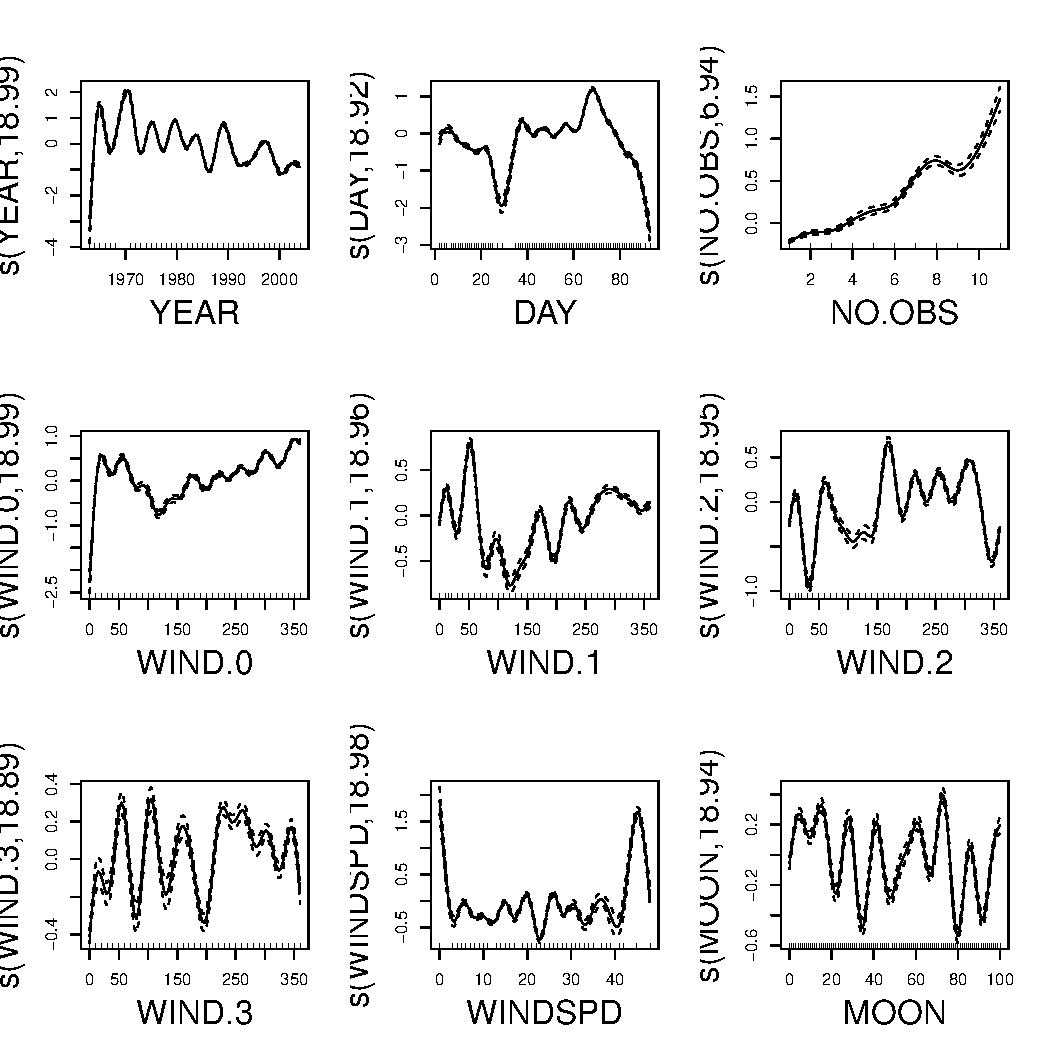
\includegraphics[width = 8cm]{figures/GrA.pdf}  
\end{center}

\end{frame}

\begin{frame}[fragile]
\frametitle{}

{\scriptsize
\begin{lstlisting}
> gam.check(GrA.fit)

Method: UBRE   Optimizer: outer newton
full convergence after 12 iterations.
Gradient range [-1.543031e-05,2.132528e-05]
(score 38.92044 & scale 1).
eigenvalue range [-1.317038e-05,8.758125e-05].
Model rank =  167 / 167 

Basis dimension (k) checking results. Low p-value (k-index<1) may
indicate that k is too low, especially if edf is close to k'.

               k'    edf k-index p-value
s(YEAR)    19.000 18.987   0.676    0.00
s(DAY)     19.000 18.923   0.838    0.00
s(NO.OBS)   7.000  6.941   0.704    0.00
s(WIND.0)  19.000 18.985   0.846    0.00
s(WIND.1)  19.000 18.962   0.894    0.00
s(WIND.2)  19.000 18.951   0.903    0.00
s(WIND.3)  19.000 18.891   0.895    0.00
s(WINDSPD) 19.000 18.982   0.888    0.00
s(MOON)    19.000 18.945   0.959    0.31
\end{lstlisting}
}
\end{frame}

\begin{frame}
\begin{center}
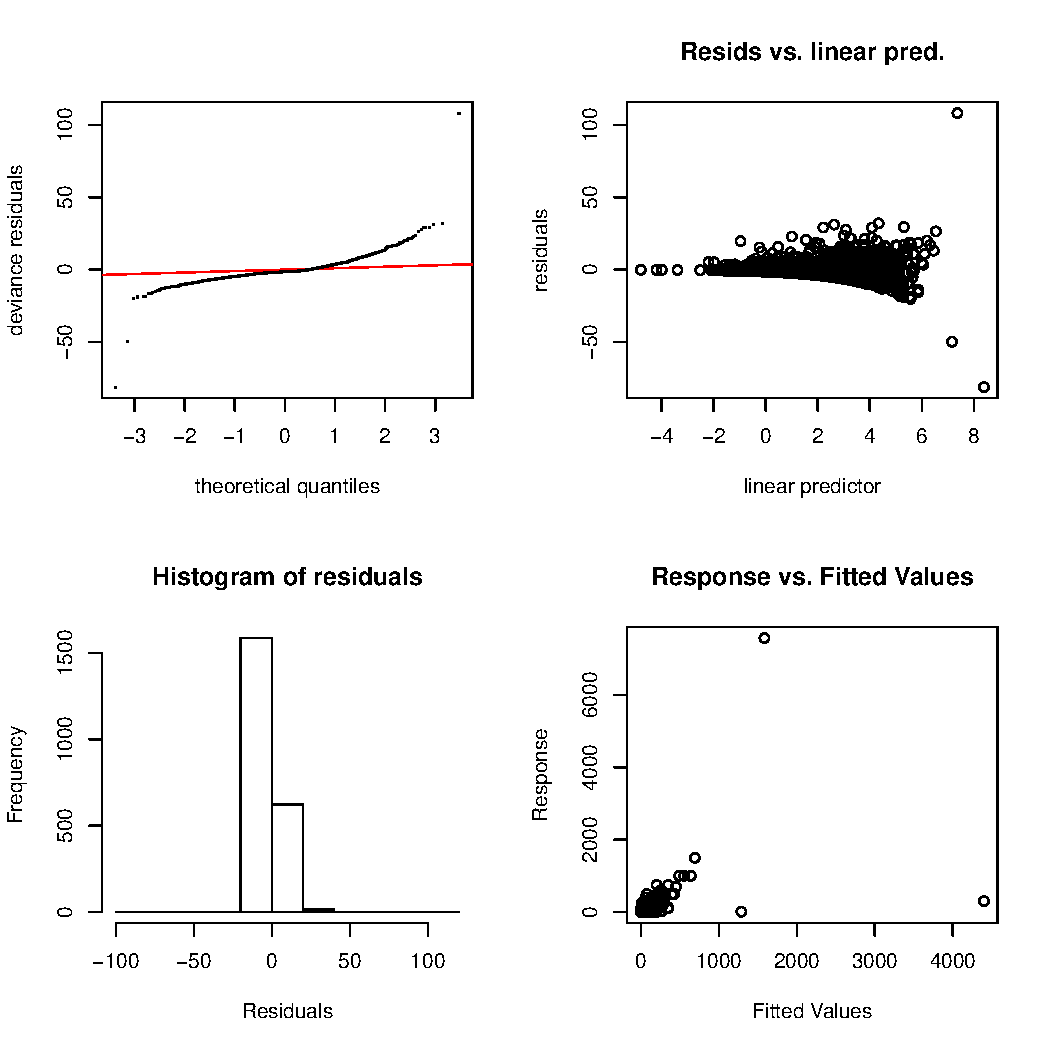
\includegraphics[width = 7.5cm]{figures/GrAcheck.pdf}  
\end{center}
\end{frame}

\begin{frame}[fragile]
\frametitle{}

{\scriptsize
\begin{lstlisting}
> summary(GrA.fit)

Family: poisson 
Link function: log 

Formula:
NUMBER ~ s(YEAR, k = 20) + s(DAY, k = 20) + s(NO.OBS, k = 8) + 
    s(WIND.0, k = 20) + s(WIND.1, k = 20) + s(WIND.2, k = 20) + 
    s(WIND.3, k = 20) + s(WINDSPD, k = 20) + factor(SKY) + s(MOON, 
    k = 20) + factor(BIRD)

Parametric coefficients:
                  Estimate Std. Error z value Pr(>|z|)    
(Intercept)        2.84578    0.01186 239.898  < 2e-16 ***
factor(SKY)cloudy  0.03137    0.01300   2.413   0.0158 *  
factor(SKY)fog    -0.04209    0.01852  -2.272   0.0231 *  
factor(SKY)rain   -0.09024    0.02229  -4.048 5.16e-05 ***
factor(BIRD)2     -2.00090    0.02604 -76.849  < 2e-16 ***
factor(BIRD)3     -2.60308    0.03415 -76.223  < 2e-16 ***
factor(BIRD)4      0.20671    0.01208  17.118  < 2e-16 ***
factor(BIRD)5      1.22781    0.01020 120.359  < 2e-16 ***
---
Signif. codes:  0 ‘***’ 0.001 ‘**’ 0.01 ‘*’ 0.05 ‘.’ 0.1 ‘ ’ 1

\end{lstlisting}
}
\end{frame}

\begin{frame}[fragile]
\frametitle{}

{\scriptsize
\begin{lstlisting}
Approximate significance of smooth terms:
              edf Ref.df Chi.sq p-value    
s(YEAR)    18.987 19.000   9207  <2e-16 ***
s(DAY)     18.923 18.999   6365  <2e-16 ***
s(NO.OBS)   6.941  6.998   1862  <2e-16 ***
s(WIND.0)  18.985 19.000   3543  <2e-16 ***
s(WIND.1)  18.962 19.000   2172  <2e-16 ***
s(WIND.2)  18.951 19.000   3784  <2e-16 ***
s(WIND.3)  18.891 18.998   1383  <2e-16 ***
s(WINDSPD) 18.982 19.000   3259  <2e-16 ***
s(MOON)    18.945 18.999   1746  <2e-16 ***
---
Signif. codes:  0 ‘***’ 0.001 ‘**’ 0.01 ‘*’ 0.05 ‘.’ 0.1 ‘ ’ 1

R-sq.(adj) =  0.0895   Deviance explained = 65.5%
UBRE =  38.92  Scale est. = 1         n = 2230
\end{lstlisting}
}
\end{frame}


\begin{frame}[fragile]
\frametitle{Quasi-poisson model, cycle basis for \texttt{WIND}}

{\scriptsize
\begin{lstlisting}
> gam.check(GrA.quasifit)
Method: GCV   Optimizer: outer newton
full convergence after 9 iterations.
Gradient range [-3.33374e-06,2.451736e-05]
(score 45.78461 & scale 58.39889).
Hessian positive definite, eigenvalue range [0.003653669,0.04407047].
Model rank =  163 / 163 

Basis dimension (k) checking results. Low p-value (k-index<1) may
indicate that k is too low, especially if edf is close to k'.
               k'    edf k-index p-value
s(YEAR)    19.000 18.819   0.685    0.00
s(DAY)     19.000 12.869   0.831    0.00
s(NO.OBS)   7.000  2.317   0.705    0.00
s(WIND.0)  18.000  9.992   0.840    0.00
s(WIND.1)  18.000  9.003   0.890    0.00
s(WIND.2)  18.000 14.793   0.908    0.00
s(WIND.3)  18.000  4.803   0.887    0.00
s(WINDSPD) 19.000 17.248   0.905    0.00
s(MOON)    19.000 16.376   0.956    0.27
\end{lstlisting}
}
\end{frame}

\begin{frame}
\begin{center}
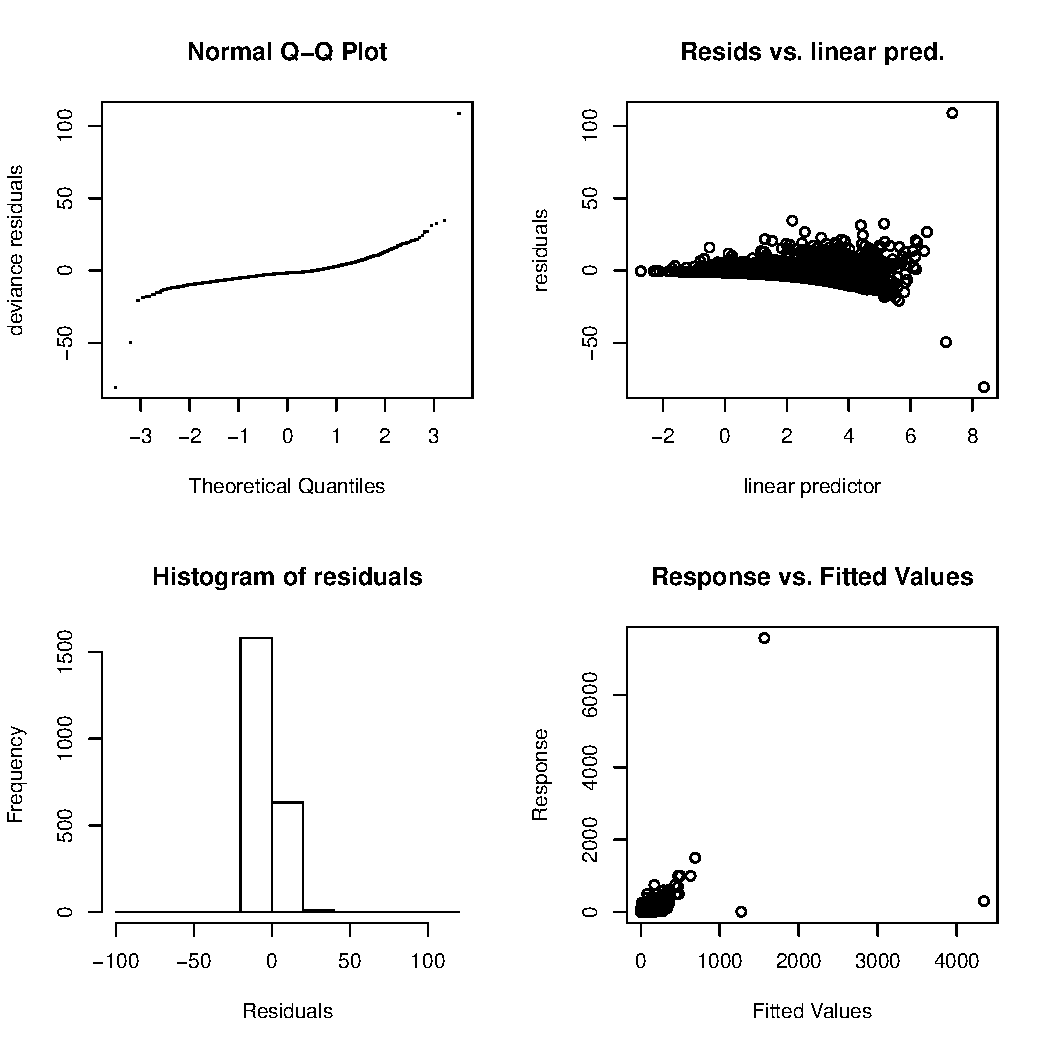
\includegraphics[width = 7.5cm]{figures/GrAquasicheck.pdf}  
\end{center}
\end{frame}

\begin{frame}[fragile]
\frametitle{}

{\scriptsize
\begin{lstlisting}
> summary(GrA.quasifit)

Family: quasipoisson 
Link function: log 

Formula:
NUMBER ~ s(YEAR, k = 30) + s(DAY, k = 30) + s(NO.OBS, k = 8) + 
    s(WIND.0, k = 30, bs = "cc") + s(WIND.1, k = 20, bs = "cc") + 
    s(WIND.2, k = 30, bs = "cc") + s(WIND.3, k = 30, bs = "cc") + 
    s(WINDSPD, k = 30) + factor(SKY) + s(MOON, k = 30) + factor(BIRD)

Parametric coefficients:
                    Estimate Std. Error t value Pr(>|t|)    
(Intercept)        2.880e+00  8.486e-02  33.940   <2e-16 ***
factor(SKY)cloudy -4.954e-05  9.023e-02  -0.001   0.9996    
factor(SKY)fog    -1.048e-02  1.310e-01  -0.080   0.9362    
factor(SKY)rain   -2.195e-01  1.541e-01  -1.425   0.1544    
factor(BIRD)2     -2.001e+00  1.916e-01 -10.444   <2e-16 ***
factor(BIRD)3     -2.603e+00  2.514e-01 -10.355   <2e-16 ***
factor(BIRD)4      2.065e-01  8.888e-02   2.324   0.0202 *  
factor(BIRD)5      1.228e+00  7.508e-02  16.356   <2e-16 ***
---
Signif. codes:  0 ‘***’ 0.001 ‘**’ 0.01 ‘*’ 0.05 ‘.’ 0.1 ‘ ’ 1
\end{lstlisting}
}
\end{frame}

\begin{frame}[fragile]
\frametitle{}

{\scriptsize
\begin{lstlisting}
Approximate significance of smooth terms:
              edf Ref.df     F  p-value    
s(YEAR)    28.697 28.964 8.007  < 2e-16 ***
s(DAY)     17.522 20.852 5.485 2.00e-14 ***
s(NO.OBS)   3.534  4.265 9.785 4.15e-08 ***
s(WIND.0)  24.510 28.000 3.388 9.87e-12 ***
s(WIND.1)   8.080 18.000 2.438 1.30e-08 ***
s(WIND.2)   2.820 28.000 0.652 3.03e-05 ***
s(WIND.3)  23.924 28.000 1.585  0.00223 ** 
s(WINDSPD)  8.943 10.887 4.105 5.99e-06 ***
s(MOON)    26.886 28.474 2.840 8.02e-07 ***
---
Signif. codes:  0 ‘***’ 0.001 ‘**’ 0.01 ‘*’ 0.05 ‘.’ 0.1 ‘ ’ 1

R-sq.(adj) =  0.103   Deviance explained =   67%
GCV = 43.889  Scale est. = 54.171    n = 2230
\end{lstlisting}
}
\end{frame}


\begin{frame}[fragile]
\frametitle{Quasi-poisson, cycle basis for \texttt{WIND}, without outlier}

{\scriptsize
\begin{lstlisting}
> gam.check(GrA.quasifit.wo)
Method: GCV   Optimizer: outer newton
full convergence after 9 iterations.
Gradient range [-2.221881e-06,2.419194e-05]
(score 32.65511 & scale 44.22684).
Hessian positive definite, eigenvalue range [0.00213954,0.02999257].
Model rank =  163 / 163 

Basis dimension (k) checking results. Low p-value (k-index<1) may
indicate that k is too low, especially if edf is close to k'.
               k'    edf k-index p-value
s(YEAR)    19.000 18.826   0.568    0.00
s(DAY)     19.000 16.152   0.841    0.00
s(NO.OBS)   7.000  1.939   0.617    0.00
s(WIND.0)  18.000  8.973   0.858    0.00
s(WIND.1)  18.000 15.711   0.920    0.02
s(WIND.2)  18.000 15.715   0.887    0.00
s(WIND.3)  18.000 15.871   0.904    0.00
s(WINDSPD) 19.000 15.680   0.910    0.00
s(MOON)    19.000 17.462   0.968    0.55
\end{lstlisting}
}
\end{frame}

\begin{frame}
\begin{center}
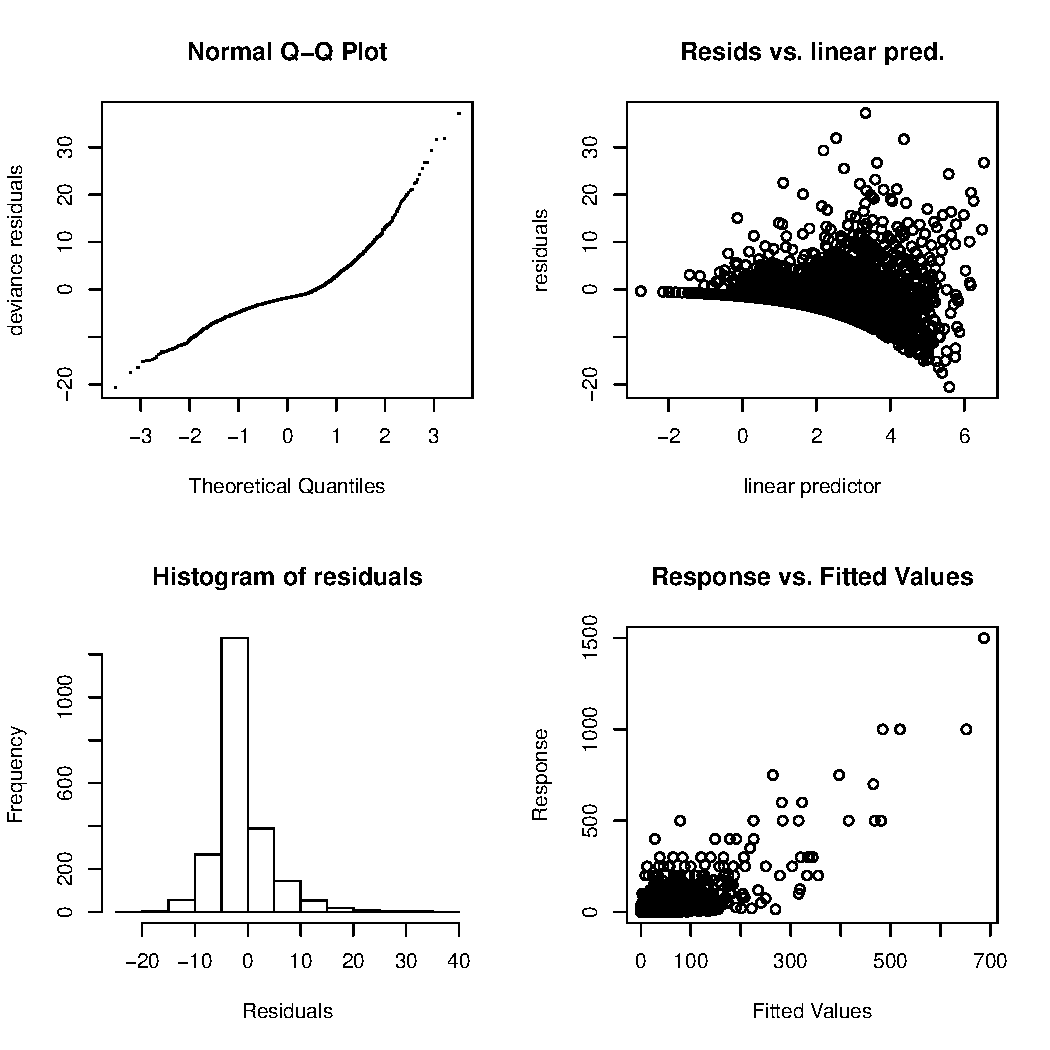
\includegraphics[width = 7.5cm]{figures/GrAquasicheckwo.pdf}  
\end{center}
\end{frame}


\begin{frame}[fragile]
\frametitle{Negative binomial, cycle basis for \texttt{WIND}, without outlier}

{\scriptsize
\begin{lstlisting}
> gam.check(GrAFitnegbin.wo)
Method: REML   Optimizer: outer newton
full convergence after 6 iterations.
Gradient range [-0.002532445,0.001774942]
(score 7125.691 & scale 1).
Hessian positive definite, eigenvalue range [0.002520513,740.6654].
Model rank =  153 / 153 

Basis dimension (k) checking results. Low p-value (k-index<1) may
indicate that k is too low, especially if edf is close to k'.
               k'    edf k-index p-value
s(YEAR)    19.000 14.481   0.356    0.00
s(DAY)     19.000  6.014   0.620    0.00
s(NO.OBS)   7.000  2.457   0.404    0.00
s(WIND.0)  18.000  3.852   0.703    0.00
s(WIND.1)  18.000  2.709   0.734    0.00
s(WIND.2)  18.000  2.182   0.689    0.00
s(WIND.3)  18.000  2.225   0.729    0.00
s(WINDSPD) 19.000  2.202   0.698    0.00
s(MOON)     9.000  1.007   0.778    0.34
\end{lstlisting}
}
\end{frame}


\begin{frame}
\begin{center}
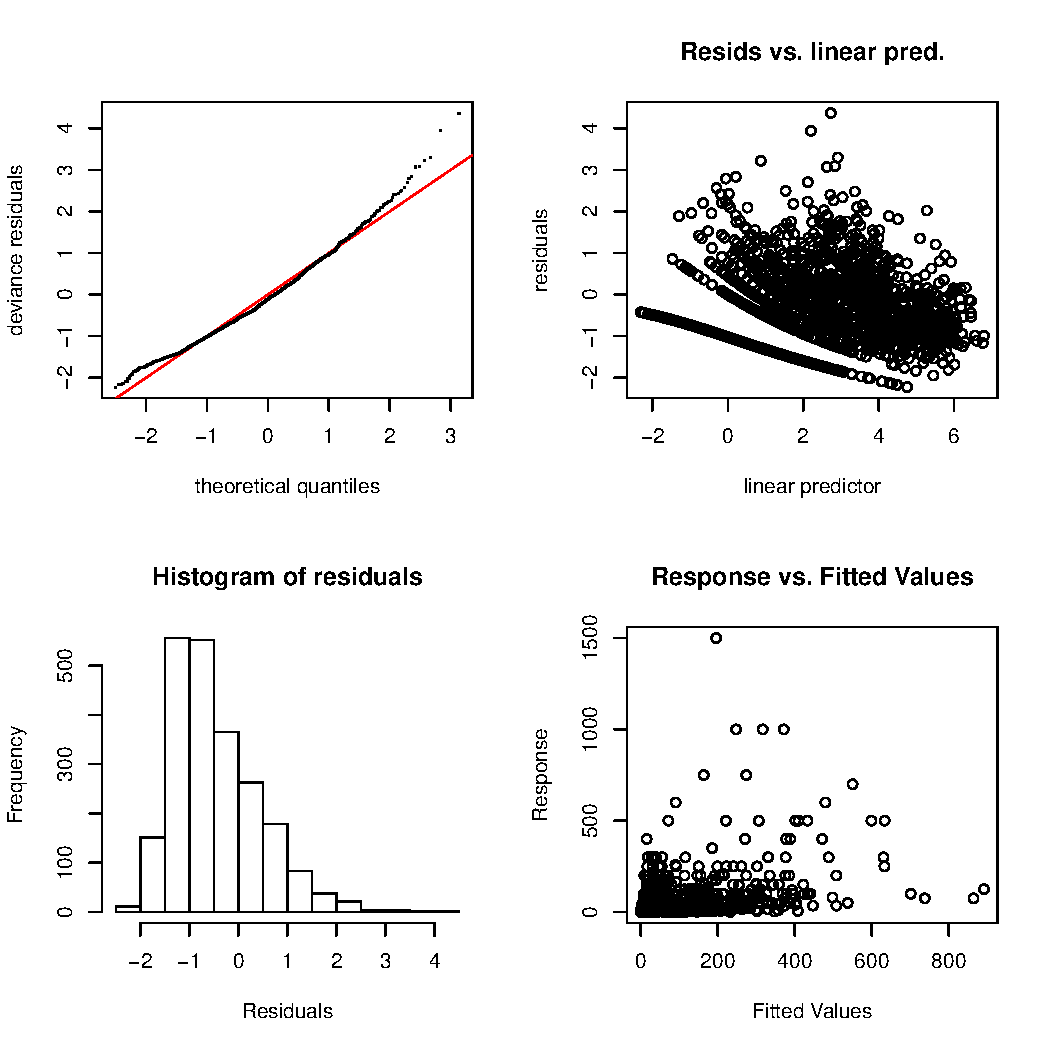
\includegraphics[width = 7.5cm]{figures/GrANBcheckwo.pdf}  
\end{center}
\end{frame}


\begin{frame}[fragile]
\frametitle{}

{\scriptsize
\begin{lstlisting}
> summary(GrAFitnegbin.wo)

Family: Negative Binomial(0.444) 
Link function: log 

Formula:
NUMBER ~ s(YEAR, k = 20) + s(DAY, k = 20) + s(NO.OBS, k = 8) + 
    s(WIND.0, k = 20, bs = "cc") + s(WIND.1, k = 20, bs = "cc") + 
    s(WIND.2, k = 20, bs = "cc") + s(WIND.3, k = 20, bs = "cc") + 
    s(WINDSPD, k = 20) + factor(SKY) + s(MOON) + factor(BIRD)

Parametric coefficients:
                  Estimate Std. Error z value Pr(>|z|)    
(Intercept)        3.15046    0.08405  37.484   <2e-16 ***
factor(SKY)cloudy -0.06807    0.08731  -0.780   0.4356    
factor(SKY)fog    -0.19088    0.11097  -1.720   0.0854 .  
factor(SKY)rain   -0.12774    0.13333  -0.958   0.3380    
factor(BIRD)2     -2.42337    0.10868 -22.298   <2e-16 ***
factor(BIRD)3     -2.98799    0.11281 -26.487   <2e-16 ***
factor(BIRD)4     -1.03015    0.10348  -9.955   <2e-16 ***
factor(BIRD)5      1.52882    0.10154  15.057   <2e-16 ***
---
Signif. codes:  0 ‘***’ 0.001 ‘**’ 0.01 ‘*’ 0.05 ‘.’ 0.1 ‘ ’ 1
\end{lstlisting}
}
\end{frame}

\begin{frame}[fragile]
\frametitle{}

{\scriptsize
\begin{lstlisting}

Approximate significance of smooth terms:
              edf Ref.df  Chi.sq  p-value    
s(YEAR)    14.481 16.591 188.028  < 2e-16 ***
s(DAY)      6.014  7.448 239.399  < 2e-16 ***
s(NO.OBS)   2.457  3.033  28.412 3.30e-06 ***
s(WIND.0)   3.852 18.000  75.064  < 2e-16 ***
s(WIND.1)   2.709 18.000  16.754 8.48e-05 ***
s(WIND.2)   2.182 18.000   9.214  0.00399 ** 
s(WIND.3)   2.225 18.000   9.895  0.00296 ** 
s(WINDSPD)  2.202  2.796  10.133  0.01661 *  
s(MOON)     1.007  1.013   0.067  0.79966    
---
Signif. codes:  0 ‘***’ 0.001 ‘**’ 0.01 ‘*’ 0.05 ‘.’ 0.1 ‘ ’ 1

R-sq.(adj) =  -0.121   Deviance explained = 52.2%
-REML = 7125.7  Scale est. = 1         n = 2229
\end{lstlisting}
}
\end{frame}


\begin{frame}
\begin{center}
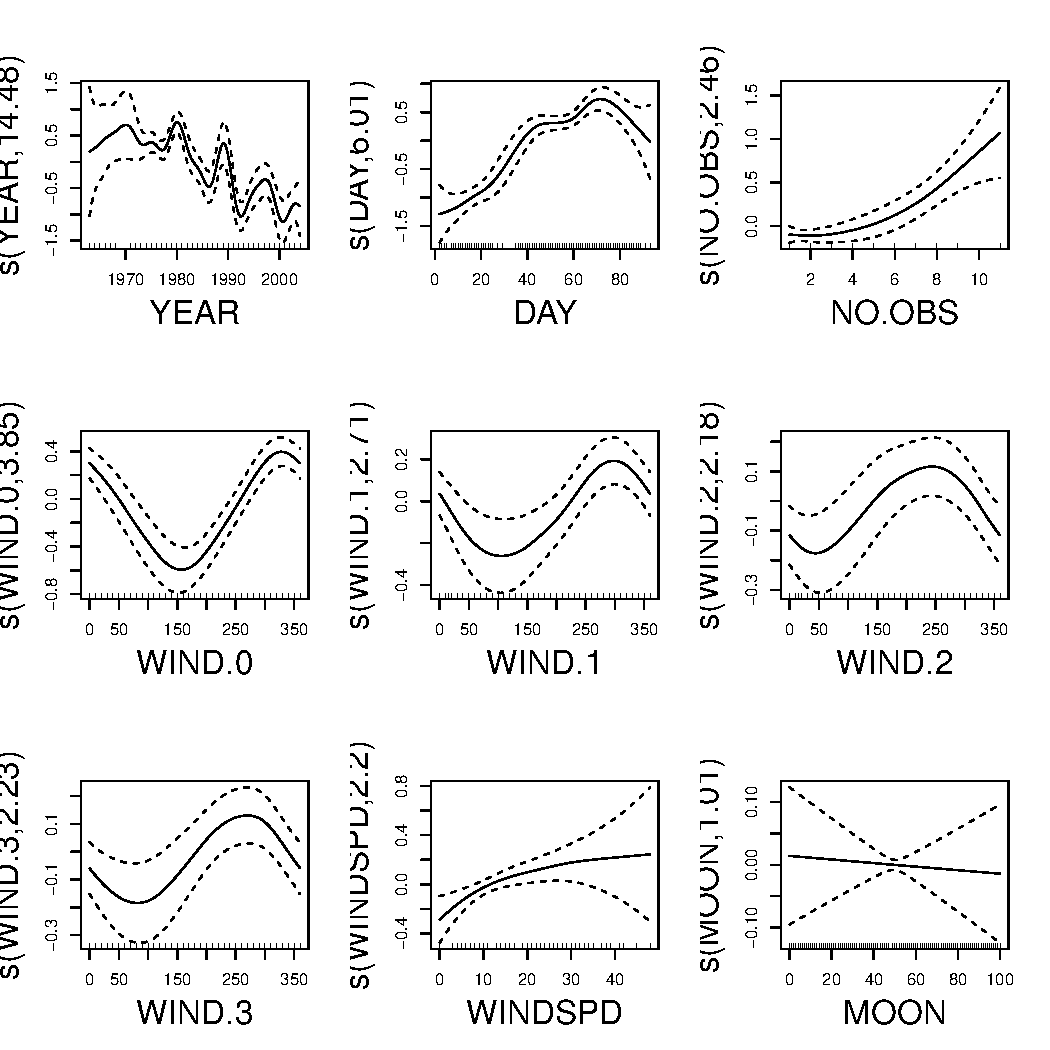
\includegraphics[width = 8cm]{figures/GrAFitnegbinwo.pdf}  
\end{center}
\end{frame}

\begin{frame}[allowframebreaks]
\frametitle{References}

{\tiny
\bibliographystyle{chicago}
\bibliography{biblio}}
\end{frame}




\end{document}

